\documentclass[twoside]{book}

% Packages required by doxygen
\usepackage{fixltx2e}
\usepackage{calc}
\usepackage{doxygen}
\usepackage[export]{adjustbox} % also loads graphicx
\usepackage{graphicx}
\usepackage[utf8]{inputenc}
\usepackage{makeidx}
\usepackage{multicol}
\usepackage{multirow}
\PassOptionsToPackage{warn}{textcomp}
\usepackage{textcomp}
\usepackage[nointegrals]{wasysym}
\usepackage[table]{xcolor}

% Font selection
\usepackage[T1]{fontenc}
\usepackage[scaled=.90]{helvet}
\usepackage{courier}
\usepackage{amssymb}
\usepackage{sectsty}
\renewcommand{\familydefault}{\sfdefault}
\allsectionsfont{%
  \fontseries{bc}\selectfont%
  \color{darkgray}%
}
\renewcommand{\DoxyLabelFont}{%
  \fontseries{bc}\selectfont%
  \color{darkgray}%
}
\newcommand{\+}{\discretionary{\mbox{\scriptsize$\hookleftarrow$}}{}{}}

% Page & text layout
\usepackage{geometry}
\geometry{%
  a4paper,%
  top=2.5cm,%
  bottom=2.5cm,%
  left=2.5cm,%
  right=2.5cm%
}
\tolerance=750
\hfuzz=15pt
\hbadness=750
\setlength{\emergencystretch}{15pt}
\setlength{\parindent}{0cm}
\setlength{\parskip}{0.2cm}
\makeatletter
\renewcommand{\paragraph}{%
  \@startsection{paragraph}{4}{0ex}{-1.0ex}{1.0ex}{%
    \normalfont\normalsize\bfseries\SS@parafont%
  }%
}
\renewcommand{\subparagraph}{%
  \@startsection{subparagraph}{5}{0ex}{-1.0ex}{1.0ex}{%
    \normalfont\normalsize\bfseries\SS@subparafont%
  }%
}
\makeatother

% Headers & footers
\usepackage{fancyhdr}
\pagestyle{fancyplain}
\fancyhead[LE]{\fancyplain{}{\bfseries\thepage}}
\fancyhead[CE]{\fancyplain{}{}}
\fancyhead[RE]{\fancyplain{}{\bfseries\leftmark}}
\fancyhead[LO]{\fancyplain{}{\bfseries\rightmark}}
\fancyhead[CO]{\fancyplain{}{}}
\fancyhead[RO]{\fancyplain{}{\bfseries\thepage}}
\fancyfoot[LE]{\fancyplain{}{}}
\fancyfoot[CE]{\fancyplain{}{}}
\fancyfoot[RE]{\fancyplain{}{\bfseries\scriptsize Generated on Thu Oct 22 2015 10\+:47\+:45 for u\+M\+Sim by Doxygen }}
\fancyfoot[LO]{\fancyplain{}{\bfseries\scriptsize Generated on Thu Oct 22 2015 10\+:47\+:45 for u\+M\+Sim by Doxygen }}
\fancyfoot[CO]{\fancyplain{}{}}
\fancyfoot[RO]{\fancyplain{}{}}
\renewcommand{\footrulewidth}{0.4pt}
\renewcommand{\chaptermark}[1]{%
  \markboth{#1}{}%
}
\renewcommand{\sectionmark}[1]{%
  \markright{\thesection\ #1}%
}

% Indices & bibliography
\usepackage{natbib}
\usepackage[titles]{tocloft}
\setcounter{tocdepth}{3}
\setcounter{secnumdepth}{5}
\makeindex

% Hyperlinks (required, but should be loaded last)
\usepackage{ifpdf}
\ifpdf
  \usepackage[pdftex,pagebackref=true]{hyperref}
\else
  \usepackage[ps2pdf,pagebackref=true]{hyperref}
\fi
\hypersetup{%
  colorlinks=true,%
  linkcolor=blue,%
  citecolor=blue,%
  unicode%
}

% Custom commands
\newcommand{\clearemptydoublepage}{%
  \newpage{\pagestyle{empty}\cleardoublepage}%
}


%===== C O N T E N T S =====

\begin{document}

% Titlepage & ToC
\hypersetup{pageanchor=false,
             bookmarks=true,
             bookmarksnumbered=true,
             pdfencoding=unicode
            }
\pagenumbering{roman}
\begin{titlepage}
\vspace*{7cm}
\begin{center}%
{\Large u\+M\+Sim \\[1ex]\large 2.\+0 }\\
\vspace*{1cm}
{\large Generated by Doxygen 1.8.10}\\
\vspace*{0.5cm}
{\small Thu Oct 22 2015 10:47:45}\\
\end{center}
\end{titlepage}
\clearemptydoublepage
\tableofcontents
\clearemptydoublepage
\pagenumbering{arabic}
\hypersetup{pageanchor=true}

%--- Begin generated contents ---
\chapter{Hierarchical Index}
\section{Class Hierarchy}
This inheritance list is sorted roughly, but not completely, alphabetically\+:\begin{DoxyCompactList}
\item G4\+User\+Event\+Action\begin{DoxyCompactList}
\item \contentsline{section}{U\+M\+Event\+Action}{\pageref{classUMEventAction}}{}
\end{DoxyCompactList}
\item G4\+User\+Run\+Action\begin{DoxyCompactList}
\item \contentsline{section}{Run\+Action}{\pageref{classRunAction}}{}
\end{DoxyCompactList}
\item G4\+V\+Hit\begin{DoxyCompactList}
\item \contentsline{section}{U\+M\+Hit}{\pageref{classUMHit}}{}
\end{DoxyCompactList}
\item G4\+V\+Modular\+Physics\+List\begin{DoxyCompactList}
\item \contentsline{section}{U\+M\+Physics\+List}{\pageref{classUMPhysicsList}}{}
\end{DoxyCompactList}
\item G4\+V\+Physics\+Constructor\begin{DoxyCompactList}
\item \contentsline{section}{Phys\+List\+Em\+Standard}{\pageref{classPhysListEmStandard}}{}
\end{DoxyCompactList}
\item G4\+V\+Sensitive\+Detector\begin{DoxyCompactList}
\item \contentsline{section}{U\+M\+S\+D}{\pageref{classUMSD}}{}
\end{DoxyCompactList}
\item G4\+V\+User\+Detector\+Construction\begin{DoxyCompactList}
\item \contentsline{section}{U\+M\+Detector\+Construction}{\pageref{classUMDetectorConstruction}}{}
\end{DoxyCompactList}
\item G4\+V\+User\+Primary\+Generator\+Action\begin{DoxyCompactList}
\item \contentsline{section}{U\+M\+Primary\+Generator\+Action}{\pageref{classUMPrimaryGeneratorAction}}{}
\end{DoxyCompactList}
\item \contentsline{section}{U\+M\+Config}{\pageref{structUMConfig}}{}
\item \contentsline{section}{U\+M\+Root\+Saver}{\pageref{classUMRootSaver}}{}
\end{DoxyCompactList}

\chapter{Data Structure Index}
\section{Data Structures}
Here are the data structures with brief descriptions\+:\begin{DoxyCompactList}
\item\contentsline{section}{\hyperlink{classPhysListEmStandard}{Phys\+List\+Em\+Standard} }{\pageref{classPhysListEmStandard}}{}
\item\contentsline{section}{\hyperlink{classRunAction}{Run\+Action} \\*The user-\/defined Run action class At the }{\pageref{classRunAction}}{}
\item\contentsline{section}{\hyperlink{structUMConfig}{U\+M\+Config} }{\pageref{structUMConfig}}{}
\item\contentsline{section}{\hyperlink{classUMDetectorConstruction}{U\+M\+Detector\+Construction} }{\pageref{classUMDetectorConstruction}}{}
\item\contentsline{section}{\hyperlink{classUMEventAction}{U\+M\+Event\+Action} }{\pageref{classUMEventAction}}{}
\item\contentsline{section}{\hyperlink{classUMHit}{U\+M\+Hit} }{\pageref{classUMHit}}{}
\item\contentsline{section}{\hyperlink{classUMPhysicsList}{U\+M\+Physics\+List} }{\pageref{classUMPhysicsList}}{}
\item\contentsline{section}{\hyperlink{classUMPrimaryGeneratorAction}{U\+M\+Primary\+Generator\+Action} }{\pageref{classUMPrimaryGeneratorAction}}{}
\item\contentsline{section}{\hyperlink{classUMRootSaver}{U\+M\+Root\+Saver} }{\pageref{classUMRootSaver}}{}
\item\contentsline{section}{\hyperlink{classUMSD}{U\+M\+S\+D} }{\pageref{classUMSD}}{}
\end{DoxyCompactList}

\chapter{File Index}
\section{File List}
Here is a list of all files with brief descriptions\+:\begin{DoxyCompactList}
\item\contentsline{section}{include/\hyperlink{PhysListEmStandard_8hh}{Phys\+List\+Em\+Standard.\+hh} }{\pageref{PhysListEmStandard_8hh}}{}
\item\contentsline{section}{include/\hyperlink{RunAction_8hh}{Run\+Action.\+hh} }{\pageref{RunAction_8hh}}{}
\item\contentsline{section}{include/\hyperlink{UMConfig_8hh}{U\+M\+Config.\+hh} }{\pageref{UMConfig_8hh}}{}
\item\contentsline{section}{include/\hyperlink{UMDetectorConstruction_8hh}{U\+M\+Detector\+Construction.\+hh} }{\pageref{UMDetectorConstruction_8hh}}{}
\item\contentsline{section}{include/\hyperlink{UMEventAction_8hh}{U\+M\+Event\+Action.\+hh} }{\pageref{UMEventAction_8hh}}{}
\item\contentsline{section}{include/\hyperlink{UMHit_8hh}{U\+M\+Hit.\+hh} }{\pageref{UMHit_8hh}}{}
\item\contentsline{section}{include/\hyperlink{UMPhysicsList_8hh}{U\+M\+Physics\+List.\+hh} }{\pageref{UMPhysicsList_8hh}}{}
\item\contentsline{section}{include/\hyperlink{UMPrimaryGeneratorAction_8hh}{U\+M\+Primary\+Generator\+Action.\+hh} }{\pageref{UMPrimaryGeneratorAction_8hh}}{}
\item\contentsline{section}{include/\hyperlink{UMRootSaver_8hh}{U\+M\+Root\+Saver.\+hh} }{\pageref{UMRootSaver_8hh}}{}
\item\contentsline{section}{include/\hyperlink{UMSD_8hh}{U\+M\+S\+D.\+hh} }{\pageref{UMSD_8hh}}{}
\item\contentsline{section}{include/\hyperlink{UMVisManager_8hh}{U\+M\+Vis\+Manager.\+hh} }{\pageref{UMVisManager_8hh}}{}
\item\contentsline{section}{src/\hyperlink{PhysListEmStandard_8cc}{Phys\+List\+Em\+Standard.\+cc} }{\pageref{PhysListEmStandard_8cc}}{}
\item\contentsline{section}{src/\hyperlink{RunAction_8cc}{Run\+Action.\+cc} }{\pageref{RunAction_8cc}}{}
\item\contentsline{section}{src/\hyperlink{UMConfig_8cc}{U\+M\+Config.\+cc} }{\pageref{UMConfig_8cc}}{}
\item\contentsline{section}{src/\hyperlink{UMDetectorConstruction_8cc}{U\+M\+Detector\+Construction.\+cc} }{\pageref{UMDetectorConstruction_8cc}}{}
\item\contentsline{section}{src/\hyperlink{UMEventAction_8cc}{U\+M\+Event\+Action.\+cc} }{\pageref{UMEventAction_8cc}}{}
\item\contentsline{section}{src/\hyperlink{UMHit_8cc}{U\+M\+Hit.\+cc} }{\pageref{UMHit_8cc}}{}
\item\contentsline{section}{src/\hyperlink{UMPhysicsList_8cc}{U\+M\+Physics\+List.\+cc} }{\pageref{UMPhysicsList_8cc}}{}
\item\contentsline{section}{src/\hyperlink{UMPrimaryGeneratorAction_8cc}{U\+M\+Primary\+Generator\+Action.\+cc} }{\pageref{UMPrimaryGeneratorAction_8cc}}{}
\item\contentsline{section}{src/\hyperlink{UMRootSaver_8cc}{U\+M\+Root\+Saver.\+cc} }{\pageref{UMRootSaver_8cc}}{}
\item\contentsline{section}{src/\hyperlink{UMSD_8cc}{U\+M\+S\+D.\+cc} }{\pageref{UMSD_8cc}}{}
\item\contentsline{section}{src/\hyperlink{UMVisManager_8cc}{U\+M\+Vis\+Manager.\+cc} }{\pageref{UMVisManager_8cc}}{}
\end{DoxyCompactList}

\chapter{Data Structure Documentation}
\hypertarget{classPhysListEmStandard}{}\section{Phys\+List\+Em\+Standard Class Reference}
\label{classPhysListEmStandard}\index{Phys\+List\+Em\+Standard@{Phys\+List\+Em\+Standard}}


{\ttfamily \#include $<$Phys\+List\+Em\+Standard.\+hh$>$}



Inheritance diagram for Phys\+List\+Em\+Standard\+:
\nopagebreak
\begin{figure}[H]
\begin{center}
\leavevmode
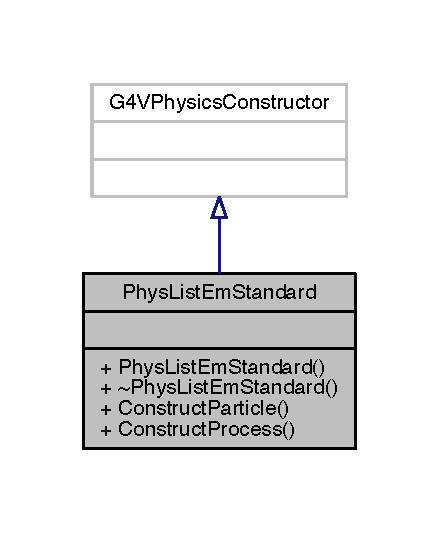
\includegraphics[width=210pt]{classPhysListEmStandard__inherit__graph}
\end{center}
\end{figure}


Collaboration diagram for Phys\+List\+Em\+Standard\+:
\nopagebreak
\begin{figure}[H]
\begin{center}
\leavevmode
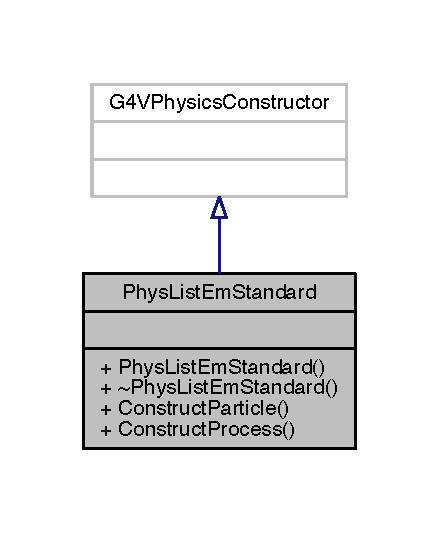
\includegraphics[width=210pt]{classPhysListEmStandard__coll__graph}
\end{center}
\end{figure}
\subsection*{Public Member Functions}
\begin{DoxyCompactItemize}
\item 
\hyperlink{classPhysListEmStandard_a014e5ba581d73a11391ec661f38204a9}{Phys\+List\+Em\+Standard} (const G4\+String \&name=\char`\"{}standard\char`\"{})
\begin{DoxyCompactList}\small\item\em Construnctor. \end{DoxyCompactList}\item 
\hyperlink{classPhysListEmStandard_a9e933bea295ed5fde8c9bc8f001cbd02}{$\sim$\+Phys\+List\+Em\+Standard} ()
\item 
void \hyperlink{classPhysListEmStandard_a4615620877453a025f908a53dcc869e8}{Construct\+Particle} ()
\begin{DoxyCompactList}\small\item\em This method is dummy for physics. \end{DoxyCompactList}\item 
void \hyperlink{classPhysListEmStandard_a81d82b49c38e371a29b03a419a417de6}{Construct\+Process} ()
\end{DoxyCompactItemize}


\subsection{Detailed Description}
Header for Electromagnetic Interactions Physics List Em\+Standard is used

\begin{DoxyAuthor}{Author}
Nikolaos Karastathis $<$ nkarast .at. cern .dot. ch $>$ 
\end{DoxyAuthor}
\begin{DoxyVersion}{Version}
v2.\+0 
\end{DoxyVersion}


\subsection{Constructor \& Destructor Documentation}
\hypertarget{classPhysListEmStandard_a014e5ba581d73a11391ec661f38204a9}{}\index{Phys\+List\+Em\+Standard@{Phys\+List\+Em\+Standard}!Phys\+List\+Em\+Standard@{Phys\+List\+Em\+Standard}}
\index{Phys\+List\+Em\+Standard@{Phys\+List\+Em\+Standard}!Phys\+List\+Em\+Standard@{Phys\+List\+Em\+Standard}}
\subsubsection[{Phys\+List\+Em\+Standard(const G4\+String \&name=""standard"")}]{\setlength{\rightskip}{0pt plus 5cm}Phys\+List\+Em\+Standard\+::\+Phys\+List\+Em\+Standard (
\begin{DoxyParamCaption}
\item[{const G4\+String \&}]{name = {\ttfamily \char`\"{}standard\char`\"{}}}
\end{DoxyParamCaption}
)}\label{classPhysListEmStandard_a014e5ba581d73a11391ec661f38204a9}


Construnctor. 

Source for \begin{DoxySeeAlso}{See also}
\hyperlink{classPhysListEmStandard}{Phys\+List\+Em\+Standard} (Shamelessly copied from a G4 example)
\end{DoxySeeAlso}
\begin{DoxyAuthor}{Author}
Nikolaos Karastathis $<$ nkarast .at. cern .dot. ch $>$ 
\end{DoxyAuthor}
\begin{DoxyVersion}{Version}
v2.\+0 
\end{DoxyVersion}
\hypertarget{classPhysListEmStandard_a9e933bea295ed5fde8c9bc8f001cbd02}{}\index{Phys\+List\+Em\+Standard@{Phys\+List\+Em\+Standard}!````~Phys\+List\+Em\+Standard@{$\sim$\+Phys\+List\+Em\+Standard}}
\index{````~Phys\+List\+Em\+Standard@{$\sim$\+Phys\+List\+Em\+Standard}!Phys\+List\+Em\+Standard@{Phys\+List\+Em\+Standard}}
\subsubsection[{$\sim$\+Phys\+List\+Em\+Standard()}]{\setlength{\rightskip}{0pt plus 5cm}Phys\+List\+Em\+Standard\+::$\sim$\+Phys\+List\+Em\+Standard (
\begin{DoxyParamCaption}
{}
\end{DoxyParamCaption}
)}\label{classPhysListEmStandard_a9e933bea295ed5fde8c9bc8f001cbd02}


\subsection{Member Function Documentation}
\hypertarget{classPhysListEmStandard_a4615620877453a025f908a53dcc869e8}{}\index{Phys\+List\+Em\+Standard@{Phys\+List\+Em\+Standard}!Construct\+Particle@{Construct\+Particle}}
\index{Construct\+Particle@{Construct\+Particle}!Phys\+List\+Em\+Standard@{Phys\+List\+Em\+Standard}}
\subsubsection[{Construct\+Particle()}]{\setlength{\rightskip}{0pt plus 5cm}void Phys\+List\+Em\+Standard\+::\+Construct\+Particle (
\begin{DoxyParamCaption}
{}
\end{DoxyParamCaption}
)\hspace{0.3cm}{\ttfamily [inline]}}\label{classPhysListEmStandard_a4615620877453a025f908a53dcc869e8}


This method is dummy for physics. 

\hypertarget{classPhysListEmStandard_a81d82b49c38e371a29b03a419a417de6}{}\index{Phys\+List\+Em\+Standard@{Phys\+List\+Em\+Standard}!Construct\+Process@{Construct\+Process}}
\index{Construct\+Process@{Construct\+Process}!Phys\+List\+Em\+Standard@{Phys\+List\+Em\+Standard}}
\subsubsection[{Construct\+Process()}]{\setlength{\rightskip}{0pt plus 5cm}void Phys\+List\+Em\+Standard\+::\+Construct\+Process (
\begin{DoxyParamCaption}
{}
\end{DoxyParamCaption}
)}\label{classPhysListEmStandard_a81d82b49c38e371a29b03a419a417de6}
This method will be invoked in the Construct() method. each physics process will be instantiated and registered to the process manager of each particle type 

The documentation for this class was generated from the following files\+:\begin{DoxyCompactItemize}
\item 
include/\hyperlink{PhysListEmStandard_8hh}{Phys\+List\+Em\+Standard.\+hh}\item 
src/\hyperlink{PhysListEmStandard_8cc}{Phys\+List\+Em\+Standard.\+cc}\end{DoxyCompactItemize}

\hypertarget{classRunAction}{}\section{Run\+Action Class Reference}
\label{classRunAction}\index{Run\+Action@{Run\+Action}}


The user-\/defined Run action class At the.  




{\ttfamily \#include $<$Run\+Action.\+hh$>$}



Inheritance diagram for Run\+Action\+:
\nopagebreak
\begin{figure}[H]
\begin{center}
\leavevmode
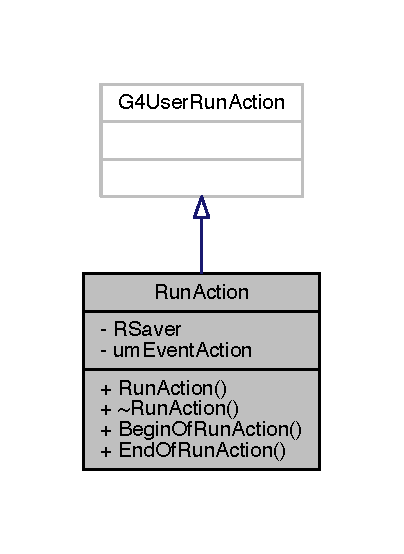
\includegraphics[width=194pt]{classRunAction__inherit__graph}
\end{center}
\end{figure}


Collaboration diagram for Run\+Action\+:
\nopagebreak
\begin{figure}[H]
\begin{center}
\leavevmode
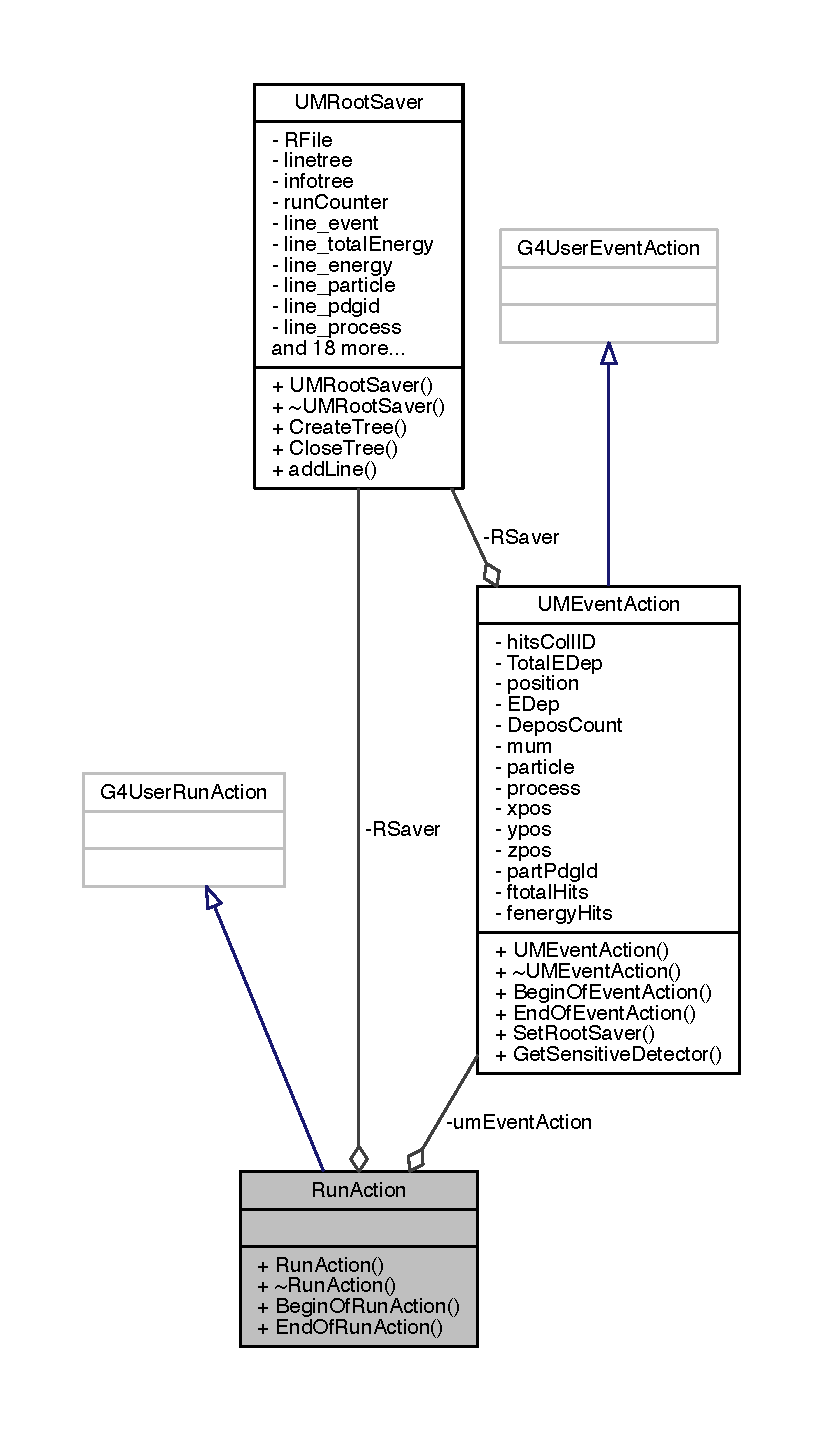
\includegraphics[height=550pt]{classRunAction__coll__graph}
\end{center}
\end{figure}
\subsection*{Public Member Functions}
\begin{DoxyCompactItemize}
\item 
\hyperlink{classRunAction_aa78ccbe310c2ff7d480d4242c2751e64}{Run\+Action} (\hyperlink{classUMEventAction}{U\+M\+Event\+Action} $\ast$ev\+Act)
\begin{DoxyCompactList}\small\item\em Constructor. \end{DoxyCompactList}\item 
virtual \hyperlink{classRunAction_a58216a98ab75d4c0d6fd8b07e2d7d710}{$\sim$\+Run\+Action} ()
\begin{DoxyCompactList}\small\item\em Destructor. \end{DoxyCompactList}\item 
void \hyperlink{classRunAction_a14b3433a6875194c4adfe1c222884f0d}{Begin\+Of\+Run\+Action} (const G4\+Run $\ast$)
\begin{DoxyCompactList}\small\item\em At the beggining of each Run execute these statements. \end{DoxyCompactList}\item 
void \hyperlink{classRunAction_a49e3c5db63358317c3babca100163bd9}{End\+Of\+Run\+Action} (const G4\+Run $\ast$)
\begin{DoxyCompactList}\small\item\em When the Run ends execute these statements. \end{DoxyCompactList}\end{DoxyCompactItemize}
\subsection*{Private Attributes}
\begin{DoxyCompactItemize}
\item 
\hyperlink{classUMRootSaver}{U\+M\+Root\+Saver} \hyperlink{classRunAction_a6628a3f063d474237f3aa7167fff359e}{R\+Saver}
\begin{DoxyCompactList}\small\item\em Link the run with the. \end{DoxyCompactList}\item 
\hyperlink{classUMEventAction}{U\+M\+Event\+Action} $\ast$ \hyperlink{classRunAction_aa9cd1a37c94536b68ef616ea87dd48f7}{um\+Event\+Action}
\begin{DoxyCompactList}\small\item\em Link to the to the. \end{DoxyCompactList}\end{DoxyCompactItemize}


\subsection{Detailed Description}
The user-\/defined Run action class At the. 

\begin{DoxySeeAlso}{See also}
\hyperlink{classRunAction_a14b3433a6875194c4adfe1c222884f0d}{Begin\+Of\+Run\+Action} a Root\+Saver object is created to store the information 
\end{DoxySeeAlso}


\subsection{Constructor \& Destructor Documentation}
\hypertarget{classRunAction_aa78ccbe310c2ff7d480d4242c2751e64}{}\index{Run\+Action@{Run\+Action}!Run\+Action@{Run\+Action}}
\index{Run\+Action@{Run\+Action}!Run\+Action@{Run\+Action}}
\subsubsection[{Run\+Action(\+U\+M\+Event\+Action $\ast$ev\+Act)}]{\setlength{\rightskip}{0pt plus 5cm}Run\+Action\+::\+Run\+Action (
\begin{DoxyParamCaption}
\item[{{\bf U\+M\+Event\+Action} $\ast$}]{the\+Event\+Action}
\end{DoxyParamCaption}
)}\label{classRunAction_aa78ccbe310c2ff7d480d4242c2751e64}


Constructor. 

Source for \begin{DoxySeeAlso}{See also}
\hyperlink{classRunAction}{Run\+Action}
\end{DoxySeeAlso}
\begin{DoxyAuthor}{Author}
Nikolaos Karastathis $<$ nkarast .at. cern .dot. ch $>$ 
\end{DoxyAuthor}
\begin{DoxyVersion}{Version}
v2.\+0 
\end{DoxyVersion}
Create an instance of Root\+Saver \hypertarget{classRunAction_a58216a98ab75d4c0d6fd8b07e2d7d710}{}\index{Run\+Action@{Run\+Action}!````~Run\+Action@{$\sim$\+Run\+Action}}
\index{````~Run\+Action@{$\sim$\+Run\+Action}!Run\+Action@{Run\+Action}}
\subsubsection[{$\sim$\+Run\+Action()}]{\setlength{\rightskip}{0pt plus 5cm}virtual Run\+Action\+::$\sim$\+Run\+Action (
\begin{DoxyParamCaption}
{}
\end{DoxyParamCaption}
)\hspace{0.3cm}{\ttfamily [inline]}, {\ttfamily [virtual]}}\label{classRunAction_a58216a98ab75d4c0d6fd8b07e2d7d710}


Destructor. 



\subsection{Member Function Documentation}
\hypertarget{classRunAction_a14b3433a6875194c4adfe1c222884f0d}{}\index{Run\+Action@{Run\+Action}!Begin\+Of\+Run\+Action@{Begin\+Of\+Run\+Action}}
\index{Begin\+Of\+Run\+Action@{Begin\+Of\+Run\+Action}!Run\+Action@{Run\+Action}}
\subsubsection[{Begin\+Of\+Run\+Action(const G4\+Run $\ast$)}]{\setlength{\rightskip}{0pt plus 5cm}void Run\+Action\+::\+Begin\+Of\+Run\+Action (
\begin{DoxyParamCaption}
\item[{const G4\+Run $\ast$}]{a\+Run}
\end{DoxyParamCaption}
)}\label{classRunAction_a14b3433a6875194c4adfe1c222884f0d}


At the beggining of each Run execute these statements. 

At the start of the Run create the R\+O\+O\+T trees. For each run a new T\+Tree is created, with default names \hypertarget{classRunAction_a49e3c5db63358317c3babca100163bd9}{}\index{Run\+Action@{Run\+Action}!End\+Of\+Run\+Action@{End\+Of\+Run\+Action}}
\index{End\+Of\+Run\+Action@{End\+Of\+Run\+Action}!Run\+Action@{Run\+Action}}
\subsubsection[{End\+Of\+Run\+Action(const G4\+Run $\ast$)}]{\setlength{\rightskip}{0pt plus 5cm}void Run\+Action\+::\+End\+Of\+Run\+Action (
\begin{DoxyParamCaption}
\item[{const G4\+Run $\ast$}]{a\+Run}
\end{DoxyParamCaption}
)}\label{classRunAction_a49e3c5db63358317c3babca100163bd9}


When the Run ends execute these statements. 

at the end of a run print out some info 

\subsection{Field Documentation}
\hypertarget{classRunAction_a6628a3f063d474237f3aa7167fff359e}{}\index{Run\+Action@{Run\+Action}!R\+Saver@{R\+Saver}}
\index{R\+Saver@{R\+Saver}!Run\+Action@{Run\+Action}}
\subsubsection[{R\+Saver}]{\setlength{\rightskip}{0pt plus 5cm}{\bf U\+M\+Root\+Saver} Run\+Action\+::\+R\+Saver\hspace{0.3cm}{\ttfamily [private]}}\label{classRunAction_a6628a3f063d474237f3aa7167fff359e}


Link the run with the. 

\begin{DoxySeeAlso}{See also}
\hyperlink{classUMRootSaver}{U\+M\+Root\+Saver} object (

\hyperlink{classRunAction_a6628a3f063d474237f3aa7167fff359e}{R\+Saver}) 
\end{DoxySeeAlso}
\hypertarget{classRunAction_aa9cd1a37c94536b68ef616ea87dd48f7}{}\index{Run\+Action@{Run\+Action}!um\+Event\+Action@{um\+Event\+Action}}
\index{um\+Event\+Action@{um\+Event\+Action}!Run\+Action@{Run\+Action}}
\subsubsection[{um\+Event\+Action}]{\setlength{\rightskip}{0pt plus 5cm}{\bf U\+M\+Event\+Action}$\ast$ Run\+Action\+::um\+Event\+Action\hspace{0.3cm}{\ttfamily [private]}}\label{classRunAction_aa9cd1a37c94536b68ef616ea87dd48f7}


Link to the to the. 

\begin{DoxySeeAlso}{See also}
\hyperlink{classUMEventAction}{U\+M\+Event\+Action} 
\end{DoxySeeAlso}


The documentation for this class was generated from the following files\+:\begin{DoxyCompactItemize}
\item 
include/\hyperlink{RunAction_8hh}{Run\+Action.\+hh}\item 
src/\hyperlink{RunAction_8cc}{Run\+Action.\+cc}\end{DoxyCompactItemize}

\hypertarget{structUMConfig}{}\section{U\+M\+Config Struct Reference}
\label{structUMConfig}\index{U\+M\+Config@{U\+M\+Config}}


{\ttfamily \#include $<$U\+M\+Config.\+hh$>$}



Collaboration diagram for U\+M\+Config\+:
\nopagebreak
\begin{figure}[H]
\begin{center}
\leavevmode
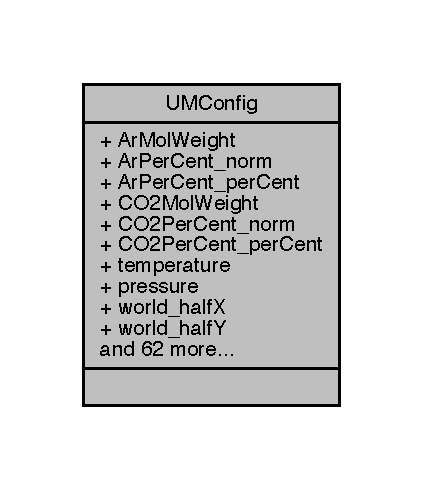
\includegraphics[width=203pt]{structUMConfig__coll__graph}
\end{center}
\end{figure}
\subsection*{Data Fields}
\begin{DoxyCompactItemize}
\item 
G4double \hyperlink{structUMConfig_a31dc39c8cb1cfdbaa648723dcd04a583}{Ar\+Mol\+Weight} = 39.\+948
\item 
G4double \hyperlink{structUMConfig_aee77ef4ee8c82ef9749ba952a4956076}{Ar\+Per\+Cent\+\_\+norm} = 0.\+93
\item 
G4double \hyperlink{structUMConfig_a0619ce16f7b8ea36806bfd25139c8a61}{Ar\+Per\+Cent\+\_\+per\+Cent} = 93.$\ast$per\+Cent
\item 
G4double \hyperlink{structUMConfig_ab4b67f65c87ddd62e28b0d49f407be31}{C\+O2\+Mol\+Weight} = 44.\+01
\item 
G4double \hyperlink{structUMConfig_ad440ec0b6c4d101ea3828d8e2834d88a}{C\+O2\+Per\+Cent\+\_\+norm} = 0.\+07
\item 
G4double \hyperlink{structUMConfig_a114afe6135ce3eabf5edb22efd2ef1ac}{C\+O2\+Per\+Cent\+\_\+per\+Cent} = 7.$\ast$per\+Cent
\item 
G4double \hyperlink{structUMConfig_ad7d3a7e160c3fe2781cee46f9be9d9fe}{temperature} = 273.\+15$\ast$kelvin
\item 
G4double \hyperlink{structUMConfig_a2c2d0d2d44efd10c2e60e8814197f95e}{pressure} = 1.$\ast$atmosphere
\item 
G4double \hyperlink{structUMConfig_ac785a055563940563f77ff0bbef41d9d}{world\+\_\+half\+X} = 250.$\ast$cm
\item 
G4double \hyperlink{structUMConfig_af679f960918ff62d3cee8a9981ffdc2c}{world\+\_\+half\+Y} = 250.$\ast$cm
\item 
G4double \hyperlink{structUMConfig_a762a80fecef0cb5fbc95edf19275cfce}{world\+\_\+half\+Z} = 250.$\ast$cm
\item 
G4double \hyperlink{structUMConfig_ab3f35a95923333ff2eedff08309662ca}{null} = 0.$\ast$um
\item 
G4double \hyperlink{structUMConfig_aeb4e8d73f0c6f7e7993e7e5af94471b4}{detector\+Vol\+\_\+half\+X} = 25000.$\ast$um
\item 
G4double \hyperlink{structUMConfig_ad7c30cbfc9df06a290bcffe70f3d8b41}{detector\+Vol\+\_\+half\+Y} = 500000.$\ast$um
\item 
G4double \hyperlink{structUMConfig_ad9353827387f9222f0dbd881b0dd2746}{detector\+Vol\+\_\+half\+Z} = 500000.$\ast$um
\item 
G4double \hyperlink{structUMConfig_a89f67c198c9542cc4421a2dc60c52b36}{pcb\+\_\+half\+X} = 1000.$\ast$um
\item 
G4double \hyperlink{structUMConfig_a6c1fe8140f1fd3613eb3d4b1f77ca13e}{pcb\+\_\+half\+Y} = 86800.$\ast$um
\item 
G4double \hyperlink{structUMConfig_a05fe3c41c98a76ff002c175229aedecc}{pcb\+\_\+half\+Z} = 86800.$\ast$um
\item 
G4double \hyperlink{structUMConfig_aafe2777462b266d6e826f29780f41734}{frame\+\_\+half\+X} = 9500.$\ast$um
\item 
G4double \hyperlink{structUMConfig_a1c381ab5ce297e813cdd3b107c3b3273}{frame\+\_\+half\+Y} = 86800.$\ast$um
\item 
G4double \hyperlink{structUMConfig_aadc0e348b160d53a5a5b86ff0574c6d0}{frame\+\_\+half\+Z} = 86800.$\ast$um
\item 
G4double \hyperlink{structUMConfig_a5904fb1d13dd60fcb6a50de8e5789340}{frame\+\_\+hole\+\_\+half\+X} = 9600.$\ast$um
\item 
G4double \hyperlink{structUMConfig_a1722d57024f27b74d518c5abf804e096}{frame\+\_\+hole\+\_\+half\+Y} = 71300.$\ast$um
\item 
G4double \hyperlink{structUMConfig_ac793ed9de1cb61e5a19e27ca6ca2bee8}{frame\+\_\+hole\+\_\+half\+Z} = 71300.$\ast$um
\item 
G4double \hyperlink{structUMConfig_a43a19c4dafb2b14f2035307cea692735}{top\+Brass\+\_\+half\+X} = 17.\+5$\ast$um
\item 
G4double \hyperlink{structUMConfig_ab11e88c0b8d6bbed643861d87ac07625}{top\+Brass\+\_\+half\+Y} = 86800.$\ast$um
\item 
G4double \hyperlink{structUMConfig_a24dd283c57244dc324355ab3dea5bdd0}{top\+Brass\+\_\+half\+Z} = 86800.$\ast$um
\item 
G4double \hyperlink{structUMConfig_a11a04ed6303378bb1f6121ae786d4805}{top\+P\+C\+B\+\_\+half\+X} = 982.\+5$\ast$um
\item 
G4double \hyperlink{structUMConfig_a33a3c114dd5c4e32308c808729bb30c3}{top\+P\+C\+B\+\_\+half\+Y} = 86800.$\ast$um
\item 
G4double \hyperlink{structUMConfig_a9b94de55cce711aedf3d05c17af0afb2}{top\+P\+C\+B\+\_\+half\+Z} = 86800.$\ast$um
\item 
G4double \hyperlink{structUMConfig_ac5be4042d6c309ebba82b98d80f86f9c}{top\+Hole\+\_\+half\+X} = 1000.$\ast$um
\item 
G4double \hyperlink{structUMConfig_ac56805f73cb5ee549501a1acc5c71ed2}{top\+Hole\+\_\+half\+Y} = 50200$\ast$um
\item 
G4double \hyperlink{structUMConfig_ab90829b627e0674333d365671c58cbb3}{top\+Hole\+\_\+half\+Z} = 50200.$\ast$um
\item 
G4double \hyperlink{structUMConfig_a5f1596eab9aa3565950c73754dda39cb}{active\+\_\+area\+\_\+half\+Y} = 50000.$\ast$um
\item 
G4double \hyperlink{structUMConfig_aa2d3a8ec4fbc8426464a7894a162be39}{active\+\_\+area\+\_\+half\+Z} = 50000.$\ast$um
\item 
G4double \hyperlink{structUMConfig_a0a439e9bae5313eae0b610d4fc48a92e}{strip\+\_\+half\+X} = 8.\+5$\ast$um
\item 
G4double \hyperlink{structUMConfig_aff9af991da94cb258f8c2c4152312c87}{strip\+\_\+half\+Y} = 75.$\ast$um
\item 
G4double \hyperlink{structUMConfig_afcaa55dfeaaf636b1e07efb7231fe079}{strip\+\_\+half\+Z} = 50000.$\ast$um
\item 
G4double \hyperlink{structUMConfig_ab675c737dc9cdc956961ce0b5af3e2f3}{strip\+\_\+pitch} = 250.$\ast$um
\item 
G4double \hyperlink{structUMConfig_ac5c60ff26c74f3d07cfabe0b028ffa1c}{glue\+\_\+block\+\_\+half\+X} = 4.$\ast$um
\item 
G4double \hyperlink{structUMConfig_a8156f7cb9cf8e37d84e14eb76822c74f}{glue\+\_\+block\+\_\+half\+Y} = 50000.$\ast$um
\item 
G4double \hyperlink{structUMConfig_a136d2f46047e3459563a35438d86fe1f}{glue\+\_\+block\+\_\+half\+Z} = 50000.$\ast$um
\item 
G4double \hyperlink{structUMConfig_ac5c105b2556a33fa698e7e8b82f9b762}{glue\+\_\+strip\+\_\+half\+X} = \hyperlink{structUMConfig_a0a439e9bae5313eae0b610d4fc48a92e}{strip\+\_\+half\+X}
\item 
G4double \hyperlink{structUMConfig_ad5188e37a8f89f27ba1c90e3ad00ed83}{glue\+\_\+strip\+\_\+half\+Y} = (\hyperlink{structUMConfig_ab675c737dc9cdc956961ce0b5af3e2f3}{strip\+\_\+pitch}-\/2.$\ast$\hyperlink{structUMConfig_aff9af991da94cb258f8c2c4152312c87}{strip\+\_\+half\+Y})/2.
\item 
G4double \hyperlink{structUMConfig_aa70a06439791fd9f4bb81ce2fc342f92}{glue\+\_\+strip\+\_\+half\+Z} = \hyperlink{structUMConfig_afcaa55dfeaaf636b1e07efb7231fe079}{strip\+\_\+half\+Z}
\item 
G4double \hyperlink{structUMConfig_aa5646f5b664fb67e9315c46d54690424}{insulator\+\_\+block\+\_\+half\+X} = 12.\+5$\ast$um
\item 
G4double \hyperlink{structUMConfig_a41c70da919e44de22920f7b1704790ca}{insulator\+\_\+block\+\_\+half\+Y} = 50000.$\ast$um
\item 
G4double \hyperlink{structUMConfig_ac37bdc75ee79cf798d480466ad3fde13}{insulator\+\_\+block\+\_\+half\+Z} = 50000.$\ast$um
\item 
G4double \hyperlink{structUMConfig_a779b130ea0412d60509556a1342071a5}{mesh\+\_\+inner\+\_\+radius} = 0.\+0$\ast$um
\item 
G4double \hyperlink{structUMConfig_a3ae6c3881d3bc76057e8fe9ffbdeaf66}{mesh\+\_\+outer\+\_\+radius} = 12.$\ast$um
\item 
G4double \hyperlink{structUMConfig_ad589fe0f446c4d020ddf0c009fe0314a}{mesh\+\_\+half\+\_\+width} = \hyperlink{structUMConfig_a5f1596eab9aa3565950c73754dda39cb}{active\+\_\+area\+\_\+half\+Y}
\item 
G4double \hyperlink{structUMConfig_a068cd29afc69e9296e6da884e7b6c4ac}{mesh\+\_\+starting\+\_\+angle} = 0.$\ast$deg
\item 
G4double \hyperlink{structUMConfig_a777f6e7384a40265f70f945c93c66820}{mesh\+\_\+spanning\+\_\+angle} = 360$\ast$deg
\item 
G4double \hyperlink{structUMConfig_a01eccb4b99640dc0d93bf74496c1184e}{mesh\+\_\+pitch} = 78.\+0$\ast$um
\item 
G4double \hyperlink{structUMConfig_abd2d64e07e405d5274f562ba81dca4ae}{amplification\+\_\+gap} = 128.$\ast$um
\item 
G4double \hyperlink{structUMConfig_aa26902f3f2f43975c6c26b2f1addc301}{drift\+\_\+gap} = 5000.$\ast$um
\item 
G4double \hyperlink{structUMConfig_aa4b9f6ec239968ac2c4b4047b7ff32c5}{pillar\+\_\+inner\+\_\+radius} = 0.\+0$\ast$deg
\item 
G4double \hyperlink{structUMConfig_ad952040a5b58ca3cbf4023319f4a2af6}{pillar\+\_\+outer\+\_\+radius} = 200.$\ast$um
\item 
G4double \hyperlink{structUMConfig_a0d4cb234021fd28b6cc327845d1db9cc}{pillar\+\_\+half\+\_\+width} = (\hyperlink{structUMConfig_abd2d64e07e405d5274f562ba81dca4ae}{amplification\+\_\+gap}-\/2$\ast$\hyperlink{structUMConfig_a0a439e9bae5313eae0b610d4fc48a92e}{strip\+\_\+half\+X}-\/\hyperlink{structUMConfig_a3ae6c3881d3bc76057e8fe9ffbdeaf66}{mesh\+\_\+outer\+\_\+radius})/2.
\item 
G4double \hyperlink{structUMConfig_a0dcfd82af061495badf0a1c322b38484}{pillar\+\_\+starting\+\_\+angle} = 0.$\ast$deg
\item 
G4double \hyperlink{structUMConfig_a6404764724906f77433b423292c7a3c0}{pillar\+\_\+spanning\+\_\+angle} = 360$\ast$deg
\item 
G4double \hyperlink{structUMConfig_a1beecce75e7f95f04f4bc28f1bb555e7}{pillar\+\_\+pitch} = 2500.\+0$\ast$um
\item 
G4double \hyperlink{structUMConfig_a01cc15c40820340a99b62ad488e8f389}{mylar\+\_\+half\+\_\+thickness} = 60$\ast$um
\item 
G4double \hyperlink{structUMConfig_a667115049ce41cb868af4d313aba742b}{pcb\+\_\+total\+\_\+thickness} = 2.$\ast$\hyperlink{structUMConfig_a89f67c198c9542cc4421a2dc60c52b36}{pcb\+\_\+half\+X}
\item 
G4double \hyperlink{structUMConfig_a940b4dce2ed84398b26316eeb1c1b35f}{frame\+\_\+total\+\_\+thickness} = 2.$\ast$(\hyperlink{structUMConfig_aafe2777462b266d6e826f29780f41734}{frame\+\_\+half\+X}+\hyperlink{structUMConfig_a43a19c4dafb2b14f2035307cea692735}{top\+Brass\+\_\+half\+X}+\hyperlink{structUMConfig_a11a04ed6303378bb1f6121ae786d4805}{top\+P\+C\+B\+\_\+half\+X}+\hyperlink{structUMConfig_a01cc15c40820340a99b62ad488e8f389}{mylar\+\_\+half\+\_\+thickness})
\item 
G4double \hyperlink{structUMConfig_a74bcad30686f23899c8b0326a30d95b0}{detector\+\_\+half\+\_\+width} = \hyperlink{structUMConfig_a6c1fe8140f1fd3613eb3d4b1f77ca13e}{pcb\+\_\+half\+Y}
\item 
G4double \hyperlink{structUMConfig_a7884fd0bd17cd4d9e5ed778187face90}{detector\+\_\+half\+\_\+height} = \hyperlink{structUMConfig_a89f67c198c9542cc4421a2dc60c52b36}{pcb\+\_\+half\+X}+\hyperlink{structUMConfig_aafe2777462b266d6e826f29780f41734}{frame\+\_\+half\+X}+\hyperlink{structUMConfig_a01cc15c40820340a99b62ad488e8f389}{mylar\+\_\+half\+\_\+thickness}+\hyperlink{structUMConfig_a11a04ed6303378bb1f6121ae786d4805}{top\+P\+C\+B\+\_\+half\+X}+\hyperlink{structUMConfig_a43a19c4dafb2b14f2035307cea692735}{top\+Brass\+\_\+half\+X}
\item 
G4\+String \hyperlink{structUMConfig_a74976964c0a3c1e31a73fd823e05bcb1}{beam\+Particle\+Name} = \char`\"{}neutron\char`\"{}
\item 
G4double \hyperlink{structUMConfig_ab02e67f7b40f3fab43e16420dc9ed66a}{beam\+Energy} = 5.\+1$\ast$Me\+V
\item 
G4double \hyperlink{structUMConfig_aefea0e00593d3272310b5f9918c411b3}{particle\+Gun\+\_\+\+Xdistance} = 183850$\ast$um
\begin{DoxyCompactList}\small\item\em \{ define the distance of the particle gun wrt to the center of the world assuming that the gun is at the center of the detector in a vertical distance of particle\+Gun\+\_\+\+Xdistance\+:\} \end{DoxyCompactList}\item 
G4double \hyperlink{structUMConfig_acd052d2268fad88072f04522ebe2ad57}{particle\+Gun\+\_\+\+Ydistance} = 0.\+0$\ast$um
\begin{DoxyCompactList}\small\item\em --26cm when inclined\+: 2x$^\wedge$2=26$^\wedge$2 -\/$>$ x=18,385cm \end{DoxyCompactList}\item 
G4double \hyperlink{structUMConfig_ac9812c1f908fee8386d07ef47c360dbb}{particle\+Gun\+\_\+\+Z\+\_\+distance} = 0.\+0$\ast$um
\end{DoxyCompactItemize}


\subsection{Detailed Description}
\char`\"{}\+Configuration\char`\"{} header for the package

\begin{DoxyAuthor}{Author}
Nikolaos Karastathis $<$ nkarast .at. cern .dot. ch $>$ 
\end{DoxyAuthor}
\begin{DoxyVersion}{Version}
v2.\+0 
\end{DoxyVersion}


\subsection{Field Documentation}
\hypertarget{structUMConfig_a5f1596eab9aa3565950c73754dda39cb}{}\index{U\+M\+Config@{U\+M\+Config}!active\+\_\+area\+\_\+half\+Y@{active\+\_\+area\+\_\+half\+Y}}
\index{active\+\_\+area\+\_\+half\+Y@{active\+\_\+area\+\_\+half\+Y}!U\+M\+Config@{U\+M\+Config}}
\subsubsection[{active\+\_\+area\+\_\+half\+Y}]{\setlength{\rightskip}{0pt plus 5cm}G4double U\+M\+Config\+::active\+\_\+area\+\_\+half\+Y = 50000.$\ast$um}\label{structUMConfig_a5f1596eab9aa3565950c73754dda39cb}
\hypertarget{structUMConfig_aa2d3a8ec4fbc8426464a7894a162be39}{}\index{U\+M\+Config@{U\+M\+Config}!active\+\_\+area\+\_\+half\+Z@{active\+\_\+area\+\_\+half\+Z}}
\index{active\+\_\+area\+\_\+half\+Z@{active\+\_\+area\+\_\+half\+Z}!U\+M\+Config@{U\+M\+Config}}
\subsubsection[{active\+\_\+area\+\_\+half\+Z}]{\setlength{\rightskip}{0pt plus 5cm}G4double U\+M\+Config\+::active\+\_\+area\+\_\+half\+Z = 50000.$\ast$um}\label{structUMConfig_aa2d3a8ec4fbc8426464a7894a162be39}
\hypertarget{structUMConfig_abd2d64e07e405d5274f562ba81dca4ae}{}\index{U\+M\+Config@{U\+M\+Config}!amplification\+\_\+gap@{amplification\+\_\+gap}}
\index{amplification\+\_\+gap@{amplification\+\_\+gap}!U\+M\+Config@{U\+M\+Config}}
\subsubsection[{amplification\+\_\+gap}]{\setlength{\rightskip}{0pt plus 5cm}G4double U\+M\+Config\+::amplification\+\_\+gap = 128.$\ast$um}\label{structUMConfig_abd2d64e07e405d5274f562ba81dca4ae}
\hypertarget{structUMConfig_a31dc39c8cb1cfdbaa648723dcd04a583}{}\index{U\+M\+Config@{U\+M\+Config}!Ar\+Mol\+Weight@{Ar\+Mol\+Weight}}
\index{Ar\+Mol\+Weight@{Ar\+Mol\+Weight}!U\+M\+Config@{U\+M\+Config}}
\subsubsection[{Ar\+Mol\+Weight}]{\setlength{\rightskip}{0pt plus 5cm}G4double U\+M\+Config\+::\+Ar\+Mol\+Weight = 39.\+948}\label{structUMConfig_a31dc39c8cb1cfdbaa648723dcd04a583}
Gas related configuration \hypertarget{structUMConfig_aee77ef4ee8c82ef9749ba952a4956076}{}\index{U\+M\+Config@{U\+M\+Config}!Ar\+Per\+Cent\+\_\+norm@{Ar\+Per\+Cent\+\_\+norm}}
\index{Ar\+Per\+Cent\+\_\+norm@{Ar\+Per\+Cent\+\_\+norm}!U\+M\+Config@{U\+M\+Config}}
\subsubsection[{Ar\+Per\+Cent\+\_\+norm}]{\setlength{\rightskip}{0pt plus 5cm}G4double U\+M\+Config\+::\+Ar\+Per\+Cent\+\_\+norm = 0.\+93}\label{structUMConfig_aee77ef4ee8c82ef9749ba952a4956076}
\hypertarget{structUMConfig_a0619ce16f7b8ea36806bfd25139c8a61}{}\index{U\+M\+Config@{U\+M\+Config}!Ar\+Per\+Cent\+\_\+per\+Cent@{Ar\+Per\+Cent\+\_\+per\+Cent}}
\index{Ar\+Per\+Cent\+\_\+per\+Cent@{Ar\+Per\+Cent\+\_\+per\+Cent}!U\+M\+Config@{U\+M\+Config}}
\subsubsection[{Ar\+Per\+Cent\+\_\+per\+Cent}]{\setlength{\rightskip}{0pt plus 5cm}G4double U\+M\+Config\+::\+Ar\+Per\+Cent\+\_\+per\+Cent = 93.$\ast$per\+Cent}\label{structUMConfig_a0619ce16f7b8ea36806bfd25139c8a61}
\hypertarget{structUMConfig_ab02e67f7b40f3fab43e16420dc9ed66a}{}\index{U\+M\+Config@{U\+M\+Config}!beam\+Energy@{beam\+Energy}}
\index{beam\+Energy@{beam\+Energy}!U\+M\+Config@{U\+M\+Config}}
\subsubsection[{beam\+Energy}]{\setlength{\rightskip}{0pt plus 5cm}G4double U\+M\+Config\+::beam\+Energy = 5.\+1$\ast$Me\+V}\label{structUMConfig_ab02e67f7b40f3fab43e16420dc9ed66a}
\hypertarget{structUMConfig_a74976964c0a3c1e31a73fd823e05bcb1}{}\index{U\+M\+Config@{U\+M\+Config}!beam\+Particle\+Name@{beam\+Particle\+Name}}
\index{beam\+Particle\+Name@{beam\+Particle\+Name}!U\+M\+Config@{U\+M\+Config}}
\subsubsection[{beam\+Particle\+Name}]{\setlength{\rightskip}{0pt plus 5cm}G4\+String U\+M\+Config\+::beam\+Particle\+Name = \char`\"{}neutron\char`\"{}}\label{structUMConfig_a74976964c0a3c1e31a73fd823e05bcb1}
Primary Generator configuration \hypertarget{structUMConfig_ab4b67f65c87ddd62e28b0d49f407be31}{}\index{U\+M\+Config@{U\+M\+Config}!C\+O2\+Mol\+Weight@{C\+O2\+Mol\+Weight}}
\index{C\+O2\+Mol\+Weight@{C\+O2\+Mol\+Weight}!U\+M\+Config@{U\+M\+Config}}
\subsubsection[{C\+O2\+Mol\+Weight}]{\setlength{\rightskip}{0pt plus 5cm}G4double U\+M\+Config\+::\+C\+O2\+Mol\+Weight = 44.\+01}\label{structUMConfig_ab4b67f65c87ddd62e28b0d49f407be31}
\hypertarget{structUMConfig_ad440ec0b6c4d101ea3828d8e2834d88a}{}\index{U\+M\+Config@{U\+M\+Config}!C\+O2\+Per\+Cent\+\_\+norm@{C\+O2\+Per\+Cent\+\_\+norm}}
\index{C\+O2\+Per\+Cent\+\_\+norm@{C\+O2\+Per\+Cent\+\_\+norm}!U\+M\+Config@{U\+M\+Config}}
\subsubsection[{C\+O2\+Per\+Cent\+\_\+norm}]{\setlength{\rightskip}{0pt plus 5cm}G4double U\+M\+Config\+::\+C\+O2\+Per\+Cent\+\_\+norm = 0.\+07}\label{structUMConfig_ad440ec0b6c4d101ea3828d8e2834d88a}
\hypertarget{structUMConfig_a114afe6135ce3eabf5edb22efd2ef1ac}{}\index{U\+M\+Config@{U\+M\+Config}!C\+O2\+Per\+Cent\+\_\+per\+Cent@{C\+O2\+Per\+Cent\+\_\+per\+Cent}}
\index{C\+O2\+Per\+Cent\+\_\+per\+Cent@{C\+O2\+Per\+Cent\+\_\+per\+Cent}!U\+M\+Config@{U\+M\+Config}}
\subsubsection[{C\+O2\+Per\+Cent\+\_\+per\+Cent}]{\setlength{\rightskip}{0pt plus 5cm}G4double U\+M\+Config\+::\+C\+O2\+Per\+Cent\+\_\+per\+Cent = 7.$\ast$per\+Cent}\label{structUMConfig_a114afe6135ce3eabf5edb22efd2ef1ac}
\hypertarget{structUMConfig_a7884fd0bd17cd4d9e5ed778187face90}{}\index{U\+M\+Config@{U\+M\+Config}!detector\+\_\+half\+\_\+height@{detector\+\_\+half\+\_\+height}}
\index{detector\+\_\+half\+\_\+height@{detector\+\_\+half\+\_\+height}!U\+M\+Config@{U\+M\+Config}}
\subsubsection[{detector\+\_\+half\+\_\+height}]{\setlength{\rightskip}{0pt plus 5cm}G4double U\+M\+Config\+::detector\+\_\+half\+\_\+height = {\bf pcb\+\_\+half\+X}+{\bf frame\+\_\+half\+X}+{\bf mylar\+\_\+half\+\_\+thickness}+{\bf top\+P\+C\+B\+\_\+half\+X}+{\bf top\+Brass\+\_\+half\+X}}\label{structUMConfig_a7884fd0bd17cd4d9e5ed778187face90}
\hypertarget{structUMConfig_a74bcad30686f23899c8b0326a30d95b0}{}\index{U\+M\+Config@{U\+M\+Config}!detector\+\_\+half\+\_\+width@{detector\+\_\+half\+\_\+width}}
\index{detector\+\_\+half\+\_\+width@{detector\+\_\+half\+\_\+width}!U\+M\+Config@{U\+M\+Config}}
\subsubsection[{detector\+\_\+half\+\_\+width}]{\setlength{\rightskip}{0pt plus 5cm}G4double U\+M\+Config\+::detector\+\_\+half\+\_\+width = {\bf pcb\+\_\+half\+Y}}\label{structUMConfig_a74bcad30686f23899c8b0326a30d95b0}
\hypertarget{structUMConfig_aeb4e8d73f0c6f7e7993e7e5af94471b4}{}\index{U\+M\+Config@{U\+M\+Config}!detector\+Vol\+\_\+half\+X@{detector\+Vol\+\_\+half\+X}}
\index{detector\+Vol\+\_\+half\+X@{detector\+Vol\+\_\+half\+X}!U\+M\+Config@{U\+M\+Config}}
\subsubsection[{detector\+Vol\+\_\+half\+X}]{\setlength{\rightskip}{0pt plus 5cm}G4double U\+M\+Config\+::detector\+Vol\+\_\+half\+X = 25000.$\ast$um}\label{structUMConfig_aeb4e8d73f0c6f7e7993e7e5af94471b4}
\hypertarget{structUMConfig_ad7c30cbfc9df06a290bcffe70f3d8b41}{}\index{U\+M\+Config@{U\+M\+Config}!detector\+Vol\+\_\+half\+Y@{detector\+Vol\+\_\+half\+Y}}
\index{detector\+Vol\+\_\+half\+Y@{detector\+Vol\+\_\+half\+Y}!U\+M\+Config@{U\+M\+Config}}
\subsubsection[{detector\+Vol\+\_\+half\+Y}]{\setlength{\rightskip}{0pt plus 5cm}G4double U\+M\+Config\+::detector\+Vol\+\_\+half\+Y = 500000.$\ast$um}\label{structUMConfig_ad7c30cbfc9df06a290bcffe70f3d8b41}
\hypertarget{structUMConfig_ad9353827387f9222f0dbd881b0dd2746}{}\index{U\+M\+Config@{U\+M\+Config}!detector\+Vol\+\_\+half\+Z@{detector\+Vol\+\_\+half\+Z}}
\index{detector\+Vol\+\_\+half\+Z@{detector\+Vol\+\_\+half\+Z}!U\+M\+Config@{U\+M\+Config}}
\subsubsection[{detector\+Vol\+\_\+half\+Z}]{\setlength{\rightskip}{0pt plus 5cm}G4double U\+M\+Config\+::detector\+Vol\+\_\+half\+Z = 500000.$\ast$um}\label{structUMConfig_ad9353827387f9222f0dbd881b0dd2746}
\hypertarget{structUMConfig_aa26902f3f2f43975c6c26b2f1addc301}{}\index{U\+M\+Config@{U\+M\+Config}!drift\+\_\+gap@{drift\+\_\+gap}}
\index{drift\+\_\+gap@{drift\+\_\+gap}!U\+M\+Config@{U\+M\+Config}}
\subsubsection[{drift\+\_\+gap}]{\setlength{\rightskip}{0pt plus 5cm}G4double U\+M\+Config\+::drift\+\_\+gap = 5000.$\ast$um}\label{structUMConfig_aa26902f3f2f43975c6c26b2f1addc301}
\hypertarget{structUMConfig_aafe2777462b266d6e826f29780f41734}{}\index{U\+M\+Config@{U\+M\+Config}!frame\+\_\+half\+X@{frame\+\_\+half\+X}}
\index{frame\+\_\+half\+X@{frame\+\_\+half\+X}!U\+M\+Config@{U\+M\+Config}}
\subsubsection[{frame\+\_\+half\+X}]{\setlength{\rightskip}{0pt plus 5cm}G4double U\+M\+Config\+::frame\+\_\+half\+X = 9500.$\ast$um}\label{structUMConfig_aafe2777462b266d6e826f29780f41734}
\hypertarget{structUMConfig_a1c381ab5ce297e813cdd3b107c3b3273}{}\index{U\+M\+Config@{U\+M\+Config}!frame\+\_\+half\+Y@{frame\+\_\+half\+Y}}
\index{frame\+\_\+half\+Y@{frame\+\_\+half\+Y}!U\+M\+Config@{U\+M\+Config}}
\subsubsection[{frame\+\_\+half\+Y}]{\setlength{\rightskip}{0pt plus 5cm}G4double U\+M\+Config\+::frame\+\_\+half\+Y = 86800.$\ast$um}\label{structUMConfig_a1c381ab5ce297e813cdd3b107c3b3273}
\hypertarget{structUMConfig_aadc0e348b160d53a5a5b86ff0574c6d0}{}\index{U\+M\+Config@{U\+M\+Config}!frame\+\_\+half\+Z@{frame\+\_\+half\+Z}}
\index{frame\+\_\+half\+Z@{frame\+\_\+half\+Z}!U\+M\+Config@{U\+M\+Config}}
\subsubsection[{frame\+\_\+half\+Z}]{\setlength{\rightskip}{0pt plus 5cm}G4double U\+M\+Config\+::frame\+\_\+half\+Z = 86800.$\ast$um}\label{structUMConfig_aadc0e348b160d53a5a5b86ff0574c6d0}
\hypertarget{structUMConfig_a5904fb1d13dd60fcb6a50de8e5789340}{}\index{U\+M\+Config@{U\+M\+Config}!frame\+\_\+hole\+\_\+half\+X@{frame\+\_\+hole\+\_\+half\+X}}
\index{frame\+\_\+hole\+\_\+half\+X@{frame\+\_\+hole\+\_\+half\+X}!U\+M\+Config@{U\+M\+Config}}
\subsubsection[{frame\+\_\+hole\+\_\+half\+X}]{\setlength{\rightskip}{0pt plus 5cm}G4double U\+M\+Config\+::frame\+\_\+hole\+\_\+half\+X = 9600.$\ast$um}\label{structUMConfig_a5904fb1d13dd60fcb6a50de8e5789340}
\hypertarget{structUMConfig_a1722d57024f27b74d518c5abf804e096}{}\index{U\+M\+Config@{U\+M\+Config}!frame\+\_\+hole\+\_\+half\+Y@{frame\+\_\+hole\+\_\+half\+Y}}
\index{frame\+\_\+hole\+\_\+half\+Y@{frame\+\_\+hole\+\_\+half\+Y}!U\+M\+Config@{U\+M\+Config}}
\subsubsection[{frame\+\_\+hole\+\_\+half\+Y}]{\setlength{\rightskip}{0pt plus 5cm}G4double U\+M\+Config\+::frame\+\_\+hole\+\_\+half\+Y = 71300.$\ast$um}\label{structUMConfig_a1722d57024f27b74d518c5abf804e096}
\hypertarget{structUMConfig_ac793ed9de1cb61e5a19e27ca6ca2bee8}{}\index{U\+M\+Config@{U\+M\+Config}!frame\+\_\+hole\+\_\+half\+Z@{frame\+\_\+hole\+\_\+half\+Z}}
\index{frame\+\_\+hole\+\_\+half\+Z@{frame\+\_\+hole\+\_\+half\+Z}!U\+M\+Config@{U\+M\+Config}}
\subsubsection[{frame\+\_\+hole\+\_\+half\+Z}]{\setlength{\rightskip}{0pt plus 5cm}G4double U\+M\+Config\+::frame\+\_\+hole\+\_\+half\+Z = 71300.$\ast$um}\label{structUMConfig_ac793ed9de1cb61e5a19e27ca6ca2bee8}
\hypertarget{structUMConfig_a940b4dce2ed84398b26316eeb1c1b35f}{}\index{U\+M\+Config@{U\+M\+Config}!frame\+\_\+total\+\_\+thickness@{frame\+\_\+total\+\_\+thickness}}
\index{frame\+\_\+total\+\_\+thickness@{frame\+\_\+total\+\_\+thickness}!U\+M\+Config@{U\+M\+Config}}
\subsubsection[{frame\+\_\+total\+\_\+thickness}]{\setlength{\rightskip}{0pt plus 5cm}G4double U\+M\+Config\+::frame\+\_\+total\+\_\+thickness = 2.$\ast$({\bf frame\+\_\+half\+X}+{\bf top\+Brass\+\_\+half\+X}+{\bf top\+P\+C\+B\+\_\+half\+X}+{\bf mylar\+\_\+half\+\_\+thickness})}\label{structUMConfig_a940b4dce2ed84398b26316eeb1c1b35f}
\hypertarget{structUMConfig_ac5c60ff26c74f3d07cfabe0b028ffa1c}{}\index{U\+M\+Config@{U\+M\+Config}!glue\+\_\+block\+\_\+half\+X@{glue\+\_\+block\+\_\+half\+X}}
\index{glue\+\_\+block\+\_\+half\+X@{glue\+\_\+block\+\_\+half\+X}!U\+M\+Config@{U\+M\+Config}}
\subsubsection[{glue\+\_\+block\+\_\+half\+X}]{\setlength{\rightskip}{0pt plus 5cm}G4double U\+M\+Config\+::glue\+\_\+block\+\_\+half\+X = 4.$\ast$um}\label{structUMConfig_ac5c60ff26c74f3d07cfabe0b028ffa1c}
\hypertarget{structUMConfig_a8156f7cb9cf8e37d84e14eb76822c74f}{}\index{U\+M\+Config@{U\+M\+Config}!glue\+\_\+block\+\_\+half\+Y@{glue\+\_\+block\+\_\+half\+Y}}
\index{glue\+\_\+block\+\_\+half\+Y@{glue\+\_\+block\+\_\+half\+Y}!U\+M\+Config@{U\+M\+Config}}
\subsubsection[{glue\+\_\+block\+\_\+half\+Y}]{\setlength{\rightskip}{0pt plus 5cm}G4double U\+M\+Config\+::glue\+\_\+block\+\_\+half\+Y = 50000.$\ast$um}\label{structUMConfig_a8156f7cb9cf8e37d84e14eb76822c74f}
\hypertarget{structUMConfig_a136d2f46047e3459563a35438d86fe1f}{}\index{U\+M\+Config@{U\+M\+Config}!glue\+\_\+block\+\_\+half\+Z@{glue\+\_\+block\+\_\+half\+Z}}
\index{glue\+\_\+block\+\_\+half\+Z@{glue\+\_\+block\+\_\+half\+Z}!U\+M\+Config@{U\+M\+Config}}
\subsubsection[{glue\+\_\+block\+\_\+half\+Z}]{\setlength{\rightskip}{0pt plus 5cm}G4double U\+M\+Config\+::glue\+\_\+block\+\_\+half\+Z = 50000.$\ast$um}\label{structUMConfig_a136d2f46047e3459563a35438d86fe1f}
\hypertarget{structUMConfig_ac5c105b2556a33fa698e7e8b82f9b762}{}\index{U\+M\+Config@{U\+M\+Config}!glue\+\_\+strip\+\_\+half\+X@{glue\+\_\+strip\+\_\+half\+X}}
\index{glue\+\_\+strip\+\_\+half\+X@{glue\+\_\+strip\+\_\+half\+X}!U\+M\+Config@{U\+M\+Config}}
\subsubsection[{glue\+\_\+strip\+\_\+half\+X}]{\setlength{\rightskip}{0pt plus 5cm}G4double U\+M\+Config\+::glue\+\_\+strip\+\_\+half\+X = {\bf strip\+\_\+half\+X}}\label{structUMConfig_ac5c105b2556a33fa698e7e8b82f9b762}
\hypertarget{structUMConfig_ad5188e37a8f89f27ba1c90e3ad00ed83}{}\index{U\+M\+Config@{U\+M\+Config}!glue\+\_\+strip\+\_\+half\+Y@{glue\+\_\+strip\+\_\+half\+Y}}
\index{glue\+\_\+strip\+\_\+half\+Y@{glue\+\_\+strip\+\_\+half\+Y}!U\+M\+Config@{U\+M\+Config}}
\subsubsection[{glue\+\_\+strip\+\_\+half\+Y}]{\setlength{\rightskip}{0pt plus 5cm}G4double U\+M\+Config\+::glue\+\_\+strip\+\_\+half\+Y = ({\bf strip\+\_\+pitch}-\/2.$\ast${\bf strip\+\_\+half\+Y})/2.}\label{structUMConfig_ad5188e37a8f89f27ba1c90e3ad00ed83}
\hypertarget{structUMConfig_aa70a06439791fd9f4bb81ce2fc342f92}{}\index{U\+M\+Config@{U\+M\+Config}!glue\+\_\+strip\+\_\+half\+Z@{glue\+\_\+strip\+\_\+half\+Z}}
\index{glue\+\_\+strip\+\_\+half\+Z@{glue\+\_\+strip\+\_\+half\+Z}!U\+M\+Config@{U\+M\+Config}}
\subsubsection[{glue\+\_\+strip\+\_\+half\+Z}]{\setlength{\rightskip}{0pt plus 5cm}G4double U\+M\+Config\+::glue\+\_\+strip\+\_\+half\+Z = {\bf strip\+\_\+half\+Z}}\label{structUMConfig_aa70a06439791fd9f4bb81ce2fc342f92}
\hypertarget{structUMConfig_aa5646f5b664fb67e9315c46d54690424}{}\index{U\+M\+Config@{U\+M\+Config}!insulator\+\_\+block\+\_\+half\+X@{insulator\+\_\+block\+\_\+half\+X}}
\index{insulator\+\_\+block\+\_\+half\+X@{insulator\+\_\+block\+\_\+half\+X}!U\+M\+Config@{U\+M\+Config}}
\subsubsection[{insulator\+\_\+block\+\_\+half\+X}]{\setlength{\rightskip}{0pt plus 5cm}G4double U\+M\+Config\+::insulator\+\_\+block\+\_\+half\+X = 12.\+5$\ast$um}\label{structUMConfig_aa5646f5b664fb67e9315c46d54690424}
\hypertarget{structUMConfig_a41c70da919e44de22920f7b1704790ca}{}\index{U\+M\+Config@{U\+M\+Config}!insulator\+\_\+block\+\_\+half\+Y@{insulator\+\_\+block\+\_\+half\+Y}}
\index{insulator\+\_\+block\+\_\+half\+Y@{insulator\+\_\+block\+\_\+half\+Y}!U\+M\+Config@{U\+M\+Config}}
\subsubsection[{insulator\+\_\+block\+\_\+half\+Y}]{\setlength{\rightskip}{0pt plus 5cm}G4double U\+M\+Config\+::insulator\+\_\+block\+\_\+half\+Y = 50000.$\ast$um}\label{structUMConfig_a41c70da919e44de22920f7b1704790ca}
\hypertarget{structUMConfig_ac37bdc75ee79cf798d480466ad3fde13}{}\index{U\+M\+Config@{U\+M\+Config}!insulator\+\_\+block\+\_\+half\+Z@{insulator\+\_\+block\+\_\+half\+Z}}
\index{insulator\+\_\+block\+\_\+half\+Z@{insulator\+\_\+block\+\_\+half\+Z}!U\+M\+Config@{U\+M\+Config}}
\subsubsection[{insulator\+\_\+block\+\_\+half\+Z}]{\setlength{\rightskip}{0pt plus 5cm}G4double U\+M\+Config\+::insulator\+\_\+block\+\_\+half\+Z = 50000.$\ast$um}\label{structUMConfig_ac37bdc75ee79cf798d480466ad3fde13}
\hypertarget{structUMConfig_ad589fe0f446c4d020ddf0c009fe0314a}{}\index{U\+M\+Config@{U\+M\+Config}!mesh\+\_\+half\+\_\+width@{mesh\+\_\+half\+\_\+width}}
\index{mesh\+\_\+half\+\_\+width@{mesh\+\_\+half\+\_\+width}!U\+M\+Config@{U\+M\+Config}}
\subsubsection[{mesh\+\_\+half\+\_\+width}]{\setlength{\rightskip}{0pt plus 5cm}G4double U\+M\+Config\+::mesh\+\_\+half\+\_\+width = {\bf active\+\_\+area\+\_\+half\+Y}}\label{structUMConfig_ad589fe0f446c4d020ddf0c009fe0314a}
\hypertarget{structUMConfig_a779b130ea0412d60509556a1342071a5}{}\index{U\+M\+Config@{U\+M\+Config}!mesh\+\_\+inner\+\_\+radius@{mesh\+\_\+inner\+\_\+radius}}
\index{mesh\+\_\+inner\+\_\+radius@{mesh\+\_\+inner\+\_\+radius}!U\+M\+Config@{U\+M\+Config}}
\subsubsection[{mesh\+\_\+inner\+\_\+radius}]{\setlength{\rightskip}{0pt plus 5cm}G4double U\+M\+Config\+::mesh\+\_\+inner\+\_\+radius = 0.\+0$\ast$um}\label{structUMConfig_a779b130ea0412d60509556a1342071a5}
\hypertarget{structUMConfig_a3ae6c3881d3bc76057e8fe9ffbdeaf66}{}\index{U\+M\+Config@{U\+M\+Config}!mesh\+\_\+outer\+\_\+radius@{mesh\+\_\+outer\+\_\+radius}}
\index{mesh\+\_\+outer\+\_\+radius@{mesh\+\_\+outer\+\_\+radius}!U\+M\+Config@{U\+M\+Config}}
\subsubsection[{mesh\+\_\+outer\+\_\+radius}]{\setlength{\rightskip}{0pt plus 5cm}G4double U\+M\+Config\+::mesh\+\_\+outer\+\_\+radius = 12.$\ast$um}\label{structUMConfig_a3ae6c3881d3bc76057e8fe9ffbdeaf66}
\hypertarget{structUMConfig_a01eccb4b99640dc0d93bf74496c1184e}{}\index{U\+M\+Config@{U\+M\+Config}!mesh\+\_\+pitch@{mesh\+\_\+pitch}}
\index{mesh\+\_\+pitch@{mesh\+\_\+pitch}!U\+M\+Config@{U\+M\+Config}}
\subsubsection[{mesh\+\_\+pitch}]{\setlength{\rightskip}{0pt plus 5cm}G4double U\+M\+Config\+::mesh\+\_\+pitch = 78.\+0$\ast$um}\label{structUMConfig_a01eccb4b99640dc0d93bf74496c1184e}
\hypertarget{structUMConfig_a777f6e7384a40265f70f945c93c66820}{}\index{U\+M\+Config@{U\+M\+Config}!mesh\+\_\+spanning\+\_\+angle@{mesh\+\_\+spanning\+\_\+angle}}
\index{mesh\+\_\+spanning\+\_\+angle@{mesh\+\_\+spanning\+\_\+angle}!U\+M\+Config@{U\+M\+Config}}
\subsubsection[{mesh\+\_\+spanning\+\_\+angle}]{\setlength{\rightskip}{0pt plus 5cm}G4double U\+M\+Config\+::mesh\+\_\+spanning\+\_\+angle = 360$\ast$deg}\label{structUMConfig_a777f6e7384a40265f70f945c93c66820}
\hypertarget{structUMConfig_a068cd29afc69e9296e6da884e7b6c4ac}{}\index{U\+M\+Config@{U\+M\+Config}!mesh\+\_\+starting\+\_\+angle@{mesh\+\_\+starting\+\_\+angle}}
\index{mesh\+\_\+starting\+\_\+angle@{mesh\+\_\+starting\+\_\+angle}!U\+M\+Config@{U\+M\+Config}}
\subsubsection[{mesh\+\_\+starting\+\_\+angle}]{\setlength{\rightskip}{0pt plus 5cm}G4double U\+M\+Config\+::mesh\+\_\+starting\+\_\+angle = 0.$\ast$deg}\label{structUMConfig_a068cd29afc69e9296e6da884e7b6c4ac}
\hypertarget{structUMConfig_a01cc15c40820340a99b62ad488e8f389}{}\index{U\+M\+Config@{U\+M\+Config}!mylar\+\_\+half\+\_\+thickness@{mylar\+\_\+half\+\_\+thickness}}
\index{mylar\+\_\+half\+\_\+thickness@{mylar\+\_\+half\+\_\+thickness}!U\+M\+Config@{U\+M\+Config}}
\subsubsection[{mylar\+\_\+half\+\_\+thickness}]{\setlength{\rightskip}{0pt plus 5cm}G4double U\+M\+Config\+::mylar\+\_\+half\+\_\+thickness = 60$\ast$um}\label{structUMConfig_a01cc15c40820340a99b62ad488e8f389}
\hypertarget{structUMConfig_ab3f35a95923333ff2eedff08309662ca}{}\index{U\+M\+Config@{U\+M\+Config}!null@{null}}
\index{null@{null}!U\+M\+Config@{U\+M\+Config}}
\subsubsection[{null}]{\setlength{\rightskip}{0pt plus 5cm}G4double U\+M\+Config\+::null = 0.$\ast$um}\label{structUMConfig_ab3f35a95923333ff2eedff08309662ca}
\hypertarget{structUMConfig_aefea0e00593d3272310b5f9918c411b3}{}\index{U\+M\+Config@{U\+M\+Config}!particle\+Gun\+\_\+\+Xdistance@{particle\+Gun\+\_\+\+Xdistance}}
\index{particle\+Gun\+\_\+\+Xdistance@{particle\+Gun\+\_\+\+Xdistance}!U\+M\+Config@{U\+M\+Config}}
\subsubsection[{particle\+Gun\+\_\+\+Xdistance}]{\setlength{\rightskip}{0pt plus 5cm}G4double U\+M\+Config\+::particle\+Gun\+\_\+\+Xdistance = 183850$\ast$um}\label{structUMConfig_aefea0e00593d3272310b5f9918c411b3}


\{ define the distance of the particle gun wrt to the center of the world assuming that the gun is at the center of the detector in a vertical distance of particle\+Gun\+\_\+\+Xdistance\+:\} 

\hypertarget{structUMConfig_acd052d2268fad88072f04522ebe2ad57}{}\index{U\+M\+Config@{U\+M\+Config}!particle\+Gun\+\_\+\+Ydistance@{particle\+Gun\+\_\+\+Ydistance}}
\index{particle\+Gun\+\_\+\+Ydistance@{particle\+Gun\+\_\+\+Ydistance}!U\+M\+Config@{U\+M\+Config}}
\subsubsection[{particle\+Gun\+\_\+\+Ydistance}]{\setlength{\rightskip}{0pt plus 5cm}G4double U\+M\+Config\+::particle\+Gun\+\_\+\+Ydistance = 0.\+0$\ast$um}\label{structUMConfig_acd052d2268fad88072f04522ebe2ad57}


--26cm when inclined\+: 2x$^\wedge$2=26$^\wedge$2 -\/$>$ x=18,385cm 

\hypertarget{structUMConfig_ac9812c1f908fee8386d07ef47c360dbb}{}\index{U\+M\+Config@{U\+M\+Config}!particle\+Gun\+\_\+\+Z\+\_\+distance@{particle\+Gun\+\_\+\+Z\+\_\+distance}}
\index{particle\+Gun\+\_\+\+Z\+\_\+distance@{particle\+Gun\+\_\+\+Z\+\_\+distance}!U\+M\+Config@{U\+M\+Config}}
\subsubsection[{particle\+Gun\+\_\+\+Z\+\_\+distance}]{\setlength{\rightskip}{0pt plus 5cm}G4double U\+M\+Config\+::particle\+Gun\+\_\+\+Z\+\_\+distance = 0.\+0$\ast$um}\label{structUMConfig_ac9812c1f908fee8386d07ef47c360dbb}
\hypertarget{structUMConfig_a89f67c198c9542cc4421a2dc60c52b36}{}\index{U\+M\+Config@{U\+M\+Config}!pcb\+\_\+half\+X@{pcb\+\_\+half\+X}}
\index{pcb\+\_\+half\+X@{pcb\+\_\+half\+X}!U\+M\+Config@{U\+M\+Config}}
\subsubsection[{pcb\+\_\+half\+X}]{\setlength{\rightskip}{0pt plus 5cm}G4double U\+M\+Config\+::pcb\+\_\+half\+X = 1000.$\ast$um}\label{structUMConfig_a89f67c198c9542cc4421a2dc60c52b36}
\hypertarget{structUMConfig_a6c1fe8140f1fd3613eb3d4b1f77ca13e}{}\index{U\+M\+Config@{U\+M\+Config}!pcb\+\_\+half\+Y@{pcb\+\_\+half\+Y}}
\index{pcb\+\_\+half\+Y@{pcb\+\_\+half\+Y}!U\+M\+Config@{U\+M\+Config}}
\subsubsection[{pcb\+\_\+half\+Y}]{\setlength{\rightskip}{0pt plus 5cm}G4double U\+M\+Config\+::pcb\+\_\+half\+Y = 86800.$\ast$um}\label{structUMConfig_a6c1fe8140f1fd3613eb3d4b1f77ca13e}
\hypertarget{structUMConfig_a05fe3c41c98a76ff002c175229aedecc}{}\index{U\+M\+Config@{U\+M\+Config}!pcb\+\_\+half\+Z@{pcb\+\_\+half\+Z}}
\index{pcb\+\_\+half\+Z@{pcb\+\_\+half\+Z}!U\+M\+Config@{U\+M\+Config}}
\subsubsection[{pcb\+\_\+half\+Z}]{\setlength{\rightskip}{0pt plus 5cm}G4double U\+M\+Config\+::pcb\+\_\+half\+Z = 86800.$\ast$um}\label{structUMConfig_a05fe3c41c98a76ff002c175229aedecc}
\hypertarget{structUMConfig_a667115049ce41cb868af4d313aba742b}{}\index{U\+M\+Config@{U\+M\+Config}!pcb\+\_\+total\+\_\+thickness@{pcb\+\_\+total\+\_\+thickness}}
\index{pcb\+\_\+total\+\_\+thickness@{pcb\+\_\+total\+\_\+thickness}!U\+M\+Config@{U\+M\+Config}}
\subsubsection[{pcb\+\_\+total\+\_\+thickness}]{\setlength{\rightskip}{0pt plus 5cm}G4double U\+M\+Config\+::pcb\+\_\+total\+\_\+thickness = 2.$\ast${\bf pcb\+\_\+half\+X}}\label{structUMConfig_a667115049ce41cb868af4d313aba742b}
\hypertarget{structUMConfig_a0d4cb234021fd28b6cc327845d1db9cc}{}\index{U\+M\+Config@{U\+M\+Config}!pillar\+\_\+half\+\_\+width@{pillar\+\_\+half\+\_\+width}}
\index{pillar\+\_\+half\+\_\+width@{pillar\+\_\+half\+\_\+width}!U\+M\+Config@{U\+M\+Config}}
\subsubsection[{pillar\+\_\+half\+\_\+width}]{\setlength{\rightskip}{0pt plus 5cm}G4double U\+M\+Config\+::pillar\+\_\+half\+\_\+width = ({\bf amplification\+\_\+gap}-\/2$\ast${\bf strip\+\_\+half\+X}-\/{\bf mesh\+\_\+outer\+\_\+radius})/2.}\label{structUMConfig_a0d4cb234021fd28b6cc327845d1db9cc}
\hypertarget{structUMConfig_aa4b9f6ec239968ac2c4b4047b7ff32c5}{}\index{U\+M\+Config@{U\+M\+Config}!pillar\+\_\+inner\+\_\+radius@{pillar\+\_\+inner\+\_\+radius}}
\index{pillar\+\_\+inner\+\_\+radius@{pillar\+\_\+inner\+\_\+radius}!U\+M\+Config@{U\+M\+Config}}
\subsubsection[{pillar\+\_\+inner\+\_\+radius}]{\setlength{\rightskip}{0pt plus 5cm}G4double U\+M\+Config\+::pillar\+\_\+inner\+\_\+radius = 0.\+0$\ast$deg}\label{structUMConfig_aa4b9f6ec239968ac2c4b4047b7ff32c5}
\hypertarget{structUMConfig_ad952040a5b58ca3cbf4023319f4a2af6}{}\index{U\+M\+Config@{U\+M\+Config}!pillar\+\_\+outer\+\_\+radius@{pillar\+\_\+outer\+\_\+radius}}
\index{pillar\+\_\+outer\+\_\+radius@{pillar\+\_\+outer\+\_\+radius}!U\+M\+Config@{U\+M\+Config}}
\subsubsection[{pillar\+\_\+outer\+\_\+radius}]{\setlength{\rightskip}{0pt plus 5cm}G4double U\+M\+Config\+::pillar\+\_\+outer\+\_\+radius = 200.$\ast$um}\label{structUMConfig_ad952040a5b58ca3cbf4023319f4a2af6}
\hypertarget{structUMConfig_a1beecce75e7f95f04f4bc28f1bb555e7}{}\index{U\+M\+Config@{U\+M\+Config}!pillar\+\_\+pitch@{pillar\+\_\+pitch}}
\index{pillar\+\_\+pitch@{pillar\+\_\+pitch}!U\+M\+Config@{U\+M\+Config}}
\subsubsection[{pillar\+\_\+pitch}]{\setlength{\rightskip}{0pt plus 5cm}G4double U\+M\+Config\+::pillar\+\_\+pitch = 2500.\+0$\ast$um}\label{structUMConfig_a1beecce75e7f95f04f4bc28f1bb555e7}
\hypertarget{structUMConfig_a6404764724906f77433b423292c7a3c0}{}\index{U\+M\+Config@{U\+M\+Config}!pillar\+\_\+spanning\+\_\+angle@{pillar\+\_\+spanning\+\_\+angle}}
\index{pillar\+\_\+spanning\+\_\+angle@{pillar\+\_\+spanning\+\_\+angle}!U\+M\+Config@{U\+M\+Config}}
\subsubsection[{pillar\+\_\+spanning\+\_\+angle}]{\setlength{\rightskip}{0pt plus 5cm}G4double U\+M\+Config\+::pillar\+\_\+spanning\+\_\+angle = 360$\ast$deg}\label{structUMConfig_a6404764724906f77433b423292c7a3c0}
\hypertarget{structUMConfig_a0dcfd82af061495badf0a1c322b38484}{}\index{U\+M\+Config@{U\+M\+Config}!pillar\+\_\+starting\+\_\+angle@{pillar\+\_\+starting\+\_\+angle}}
\index{pillar\+\_\+starting\+\_\+angle@{pillar\+\_\+starting\+\_\+angle}!U\+M\+Config@{U\+M\+Config}}
\subsubsection[{pillar\+\_\+starting\+\_\+angle}]{\setlength{\rightskip}{0pt plus 5cm}G4double U\+M\+Config\+::pillar\+\_\+starting\+\_\+angle = 0.$\ast$deg}\label{structUMConfig_a0dcfd82af061495badf0a1c322b38484}
\hypertarget{structUMConfig_a2c2d0d2d44efd10c2e60e8814197f95e}{}\index{U\+M\+Config@{U\+M\+Config}!pressure@{pressure}}
\index{pressure@{pressure}!U\+M\+Config@{U\+M\+Config}}
\subsubsection[{pressure}]{\setlength{\rightskip}{0pt plus 5cm}G4double U\+M\+Config\+::pressure = 1.$\ast$atmosphere}\label{structUMConfig_a2c2d0d2d44efd10c2e60e8814197f95e}
\hypertarget{structUMConfig_a0a439e9bae5313eae0b610d4fc48a92e}{}\index{U\+M\+Config@{U\+M\+Config}!strip\+\_\+half\+X@{strip\+\_\+half\+X}}
\index{strip\+\_\+half\+X@{strip\+\_\+half\+X}!U\+M\+Config@{U\+M\+Config}}
\subsubsection[{strip\+\_\+half\+X}]{\setlength{\rightskip}{0pt plus 5cm}G4double U\+M\+Config\+::strip\+\_\+half\+X = 8.\+5$\ast$um}\label{structUMConfig_a0a439e9bae5313eae0b610d4fc48a92e}
\hypertarget{structUMConfig_aff9af991da94cb258f8c2c4152312c87}{}\index{U\+M\+Config@{U\+M\+Config}!strip\+\_\+half\+Y@{strip\+\_\+half\+Y}}
\index{strip\+\_\+half\+Y@{strip\+\_\+half\+Y}!U\+M\+Config@{U\+M\+Config}}
\subsubsection[{strip\+\_\+half\+Y}]{\setlength{\rightskip}{0pt plus 5cm}G4double U\+M\+Config\+::strip\+\_\+half\+Y = 75.$\ast$um}\label{structUMConfig_aff9af991da94cb258f8c2c4152312c87}
\hypertarget{structUMConfig_afcaa55dfeaaf636b1e07efb7231fe079}{}\index{U\+M\+Config@{U\+M\+Config}!strip\+\_\+half\+Z@{strip\+\_\+half\+Z}}
\index{strip\+\_\+half\+Z@{strip\+\_\+half\+Z}!U\+M\+Config@{U\+M\+Config}}
\subsubsection[{strip\+\_\+half\+Z}]{\setlength{\rightskip}{0pt plus 5cm}G4double U\+M\+Config\+::strip\+\_\+half\+Z = 50000.$\ast$um}\label{structUMConfig_afcaa55dfeaaf636b1e07efb7231fe079}
\hypertarget{structUMConfig_ab675c737dc9cdc956961ce0b5af3e2f3}{}\index{U\+M\+Config@{U\+M\+Config}!strip\+\_\+pitch@{strip\+\_\+pitch}}
\index{strip\+\_\+pitch@{strip\+\_\+pitch}!U\+M\+Config@{U\+M\+Config}}
\subsubsection[{strip\+\_\+pitch}]{\setlength{\rightskip}{0pt plus 5cm}G4double U\+M\+Config\+::strip\+\_\+pitch = 250.$\ast$um}\label{structUMConfig_ab675c737dc9cdc956961ce0b5af3e2f3}
\hypertarget{structUMConfig_ad7d3a7e160c3fe2781cee46f9be9d9fe}{}\index{U\+M\+Config@{U\+M\+Config}!temperature@{temperature}}
\index{temperature@{temperature}!U\+M\+Config@{U\+M\+Config}}
\subsubsection[{temperature}]{\setlength{\rightskip}{0pt plus 5cm}G4double U\+M\+Config\+::temperature = 273.\+15$\ast$kelvin}\label{structUMConfig_ad7d3a7e160c3fe2781cee46f9be9d9fe}
\hypertarget{structUMConfig_a43a19c4dafb2b14f2035307cea692735}{}\index{U\+M\+Config@{U\+M\+Config}!top\+Brass\+\_\+half\+X@{top\+Brass\+\_\+half\+X}}
\index{top\+Brass\+\_\+half\+X@{top\+Brass\+\_\+half\+X}!U\+M\+Config@{U\+M\+Config}}
\subsubsection[{top\+Brass\+\_\+half\+X}]{\setlength{\rightskip}{0pt plus 5cm}G4double U\+M\+Config\+::top\+Brass\+\_\+half\+X = 17.\+5$\ast$um}\label{structUMConfig_a43a19c4dafb2b14f2035307cea692735}
\hypertarget{structUMConfig_ab11e88c0b8d6bbed643861d87ac07625}{}\index{U\+M\+Config@{U\+M\+Config}!top\+Brass\+\_\+half\+Y@{top\+Brass\+\_\+half\+Y}}
\index{top\+Brass\+\_\+half\+Y@{top\+Brass\+\_\+half\+Y}!U\+M\+Config@{U\+M\+Config}}
\subsubsection[{top\+Brass\+\_\+half\+Y}]{\setlength{\rightskip}{0pt plus 5cm}G4double U\+M\+Config\+::top\+Brass\+\_\+half\+Y = 86800.$\ast$um}\label{structUMConfig_ab11e88c0b8d6bbed643861d87ac07625}
\hypertarget{structUMConfig_a24dd283c57244dc324355ab3dea5bdd0}{}\index{U\+M\+Config@{U\+M\+Config}!top\+Brass\+\_\+half\+Z@{top\+Brass\+\_\+half\+Z}}
\index{top\+Brass\+\_\+half\+Z@{top\+Brass\+\_\+half\+Z}!U\+M\+Config@{U\+M\+Config}}
\subsubsection[{top\+Brass\+\_\+half\+Z}]{\setlength{\rightskip}{0pt plus 5cm}G4double U\+M\+Config\+::top\+Brass\+\_\+half\+Z = 86800.$\ast$um}\label{structUMConfig_a24dd283c57244dc324355ab3dea5bdd0}
\hypertarget{structUMConfig_ac5be4042d6c309ebba82b98d80f86f9c}{}\index{U\+M\+Config@{U\+M\+Config}!top\+Hole\+\_\+half\+X@{top\+Hole\+\_\+half\+X}}
\index{top\+Hole\+\_\+half\+X@{top\+Hole\+\_\+half\+X}!U\+M\+Config@{U\+M\+Config}}
\subsubsection[{top\+Hole\+\_\+half\+X}]{\setlength{\rightskip}{0pt plus 5cm}G4double U\+M\+Config\+::top\+Hole\+\_\+half\+X = 1000.$\ast$um}\label{structUMConfig_ac5be4042d6c309ebba82b98d80f86f9c}
\hypertarget{structUMConfig_ac56805f73cb5ee549501a1acc5c71ed2}{}\index{U\+M\+Config@{U\+M\+Config}!top\+Hole\+\_\+half\+Y@{top\+Hole\+\_\+half\+Y}}
\index{top\+Hole\+\_\+half\+Y@{top\+Hole\+\_\+half\+Y}!U\+M\+Config@{U\+M\+Config}}
\subsubsection[{top\+Hole\+\_\+half\+Y}]{\setlength{\rightskip}{0pt plus 5cm}G4double U\+M\+Config\+::top\+Hole\+\_\+half\+Y = 50200$\ast$um}\label{structUMConfig_ac56805f73cb5ee549501a1acc5c71ed2}
\hypertarget{structUMConfig_ab90829b627e0674333d365671c58cbb3}{}\index{U\+M\+Config@{U\+M\+Config}!top\+Hole\+\_\+half\+Z@{top\+Hole\+\_\+half\+Z}}
\index{top\+Hole\+\_\+half\+Z@{top\+Hole\+\_\+half\+Z}!U\+M\+Config@{U\+M\+Config}}
\subsubsection[{top\+Hole\+\_\+half\+Z}]{\setlength{\rightskip}{0pt plus 5cm}G4double U\+M\+Config\+::top\+Hole\+\_\+half\+Z = 50200.$\ast$um}\label{structUMConfig_ab90829b627e0674333d365671c58cbb3}
\hypertarget{structUMConfig_a11a04ed6303378bb1f6121ae786d4805}{}\index{U\+M\+Config@{U\+M\+Config}!top\+P\+C\+B\+\_\+half\+X@{top\+P\+C\+B\+\_\+half\+X}}
\index{top\+P\+C\+B\+\_\+half\+X@{top\+P\+C\+B\+\_\+half\+X}!U\+M\+Config@{U\+M\+Config}}
\subsubsection[{top\+P\+C\+B\+\_\+half\+X}]{\setlength{\rightskip}{0pt plus 5cm}G4double U\+M\+Config\+::top\+P\+C\+B\+\_\+half\+X = 982.\+5$\ast$um}\label{structUMConfig_a11a04ed6303378bb1f6121ae786d4805}
\hypertarget{structUMConfig_a33a3c114dd5c4e32308c808729bb30c3}{}\index{U\+M\+Config@{U\+M\+Config}!top\+P\+C\+B\+\_\+half\+Y@{top\+P\+C\+B\+\_\+half\+Y}}
\index{top\+P\+C\+B\+\_\+half\+Y@{top\+P\+C\+B\+\_\+half\+Y}!U\+M\+Config@{U\+M\+Config}}
\subsubsection[{top\+P\+C\+B\+\_\+half\+Y}]{\setlength{\rightskip}{0pt plus 5cm}G4double U\+M\+Config\+::top\+P\+C\+B\+\_\+half\+Y = 86800.$\ast$um}\label{structUMConfig_a33a3c114dd5c4e32308c808729bb30c3}
\hypertarget{structUMConfig_a9b94de55cce711aedf3d05c17af0afb2}{}\index{U\+M\+Config@{U\+M\+Config}!top\+P\+C\+B\+\_\+half\+Z@{top\+P\+C\+B\+\_\+half\+Z}}
\index{top\+P\+C\+B\+\_\+half\+Z@{top\+P\+C\+B\+\_\+half\+Z}!U\+M\+Config@{U\+M\+Config}}
\subsubsection[{top\+P\+C\+B\+\_\+half\+Z}]{\setlength{\rightskip}{0pt plus 5cm}G4double U\+M\+Config\+::top\+P\+C\+B\+\_\+half\+Z = 86800.$\ast$um}\label{structUMConfig_a9b94de55cce711aedf3d05c17af0afb2}
\hypertarget{structUMConfig_ac785a055563940563f77ff0bbef41d9d}{}\index{U\+M\+Config@{U\+M\+Config}!world\+\_\+half\+X@{world\+\_\+half\+X}}
\index{world\+\_\+half\+X@{world\+\_\+half\+X}!U\+M\+Config@{U\+M\+Config}}
\subsubsection[{world\+\_\+half\+X}]{\setlength{\rightskip}{0pt plus 5cm}G4double U\+M\+Config\+::world\+\_\+half\+X = 250.$\ast$cm}\label{structUMConfig_ac785a055563940563f77ff0bbef41d9d}
Geometry related configuration \hypertarget{structUMConfig_af679f960918ff62d3cee8a9981ffdc2c}{}\index{U\+M\+Config@{U\+M\+Config}!world\+\_\+half\+Y@{world\+\_\+half\+Y}}
\index{world\+\_\+half\+Y@{world\+\_\+half\+Y}!U\+M\+Config@{U\+M\+Config}}
\subsubsection[{world\+\_\+half\+Y}]{\setlength{\rightskip}{0pt plus 5cm}G4double U\+M\+Config\+::world\+\_\+half\+Y = 250.$\ast$cm}\label{structUMConfig_af679f960918ff62d3cee8a9981ffdc2c}
\hypertarget{structUMConfig_a762a80fecef0cb5fbc95edf19275cfce}{}\index{U\+M\+Config@{U\+M\+Config}!world\+\_\+half\+Z@{world\+\_\+half\+Z}}
\index{world\+\_\+half\+Z@{world\+\_\+half\+Z}!U\+M\+Config@{U\+M\+Config}}
\subsubsection[{world\+\_\+half\+Z}]{\setlength{\rightskip}{0pt plus 5cm}G4double U\+M\+Config\+::world\+\_\+half\+Z = 250.$\ast$cm}\label{structUMConfig_a762a80fecef0cb5fbc95edf19275cfce}


The documentation for this struct was generated from the following file\+:\begin{DoxyCompactItemize}
\item 
include/\hyperlink{UMConfig_8hh}{U\+M\+Config.\+hh}\end{DoxyCompactItemize}

\hypertarget{classUMDetectorConstruction}{}\section{U\+M\+Detector\+Construction Class Reference}
\label{classUMDetectorConstruction}\index{U\+M\+Detector\+Construction@{U\+M\+Detector\+Construction}}


{\ttfamily \#include $<$U\+M\+Detector\+Construction.\+hh$>$}



Inheritance diagram for U\+M\+Detector\+Construction\+:
\nopagebreak
\begin{figure}[H]
\begin{center}
\leavevmode
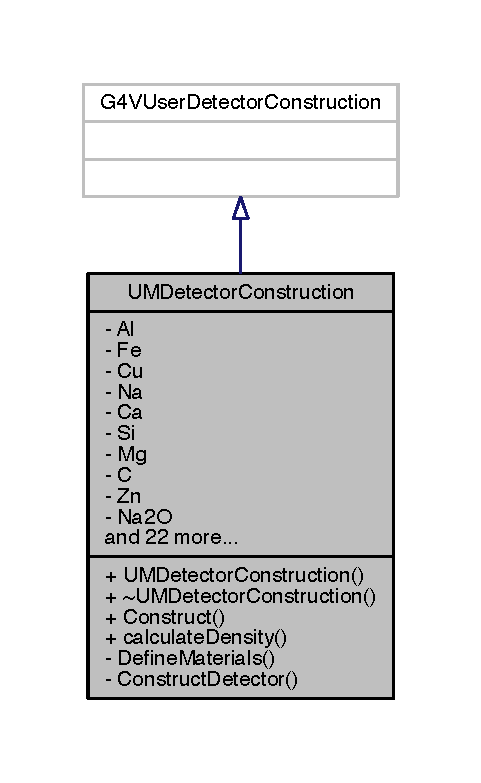
\includegraphics[width=231pt]{classUMDetectorConstruction__inherit__graph}
\end{center}
\end{figure}


Collaboration diagram for U\+M\+Detector\+Construction\+:
\nopagebreak
\begin{figure}[H]
\begin{center}
\leavevmode
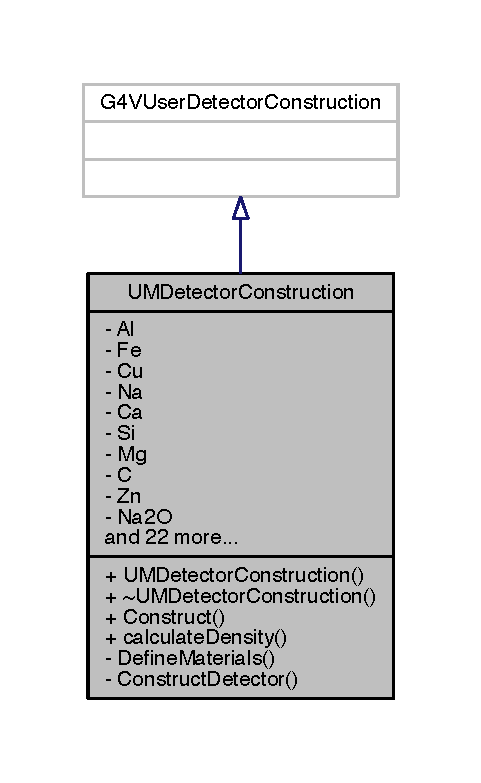
\includegraphics[width=231pt]{classUMDetectorConstruction__coll__graph}
\end{center}
\end{figure}
\subsection*{Public Member Functions}
\begin{DoxyCompactItemize}
\item 
\hyperlink{classUMDetectorConstruction_aa8795834e193baddddffe705108a0679}{U\+M\+Detector\+Construction} ()
\item 
\hyperlink{classUMDetectorConstruction_a768e4d33116b75dc4a4d48eaff6dd7ae}{$\sim$\+U\+M\+Detector\+Construction} ()
\begin{DoxyCompactList}\small\item\em Destructor. \end{DoxyCompactList}\item 
G4\+V\+Physical\+Volume $\ast$ \hyperlink{classUMDetectorConstruction_afc5538d03478fa25e9cf4337253f7d6f}{Construct} ()
\begin{DoxyCompactList}\small\item\em Construct the detector! \end{DoxyCompactList}\item 
G4double \hyperlink{classUMDetectorConstruction_ab95efe22580d366e69d32811b827a715}{calculate\+Density} (G4double mol\+Weight\+A, G4double per\+Cent\+A, G4double mol\+Weight\+B, G4double per\+Cent\+B)
\begin{DoxyCompactList}\small\item\em Calculates the density of a mixture of gasses given the relative molecular weight and the percentage. \end{DoxyCompactList}\end{DoxyCompactItemize}
\subsection*{Private Member Functions}
\begin{DoxyCompactItemize}
\item 
void \hyperlink{classUMDetectorConstruction_a06c0dcd8d247b0dc44b1081b36136da6}{Define\+Materials} ()
\item 
G4\+V\+Physical\+Volume $\ast$ \hyperlink{classUMDetectorConstruction_a5fd78be152534079d835da2c6a52c446}{Construct\+Detector} ()
\begin{DoxyCompactList}\small\item\em Construct the detector. \end{DoxyCompactList}\end{DoxyCompactItemize}
\subsection*{Private Attributes}
\begin{DoxyCompactItemize}
\item 
G4\+Material $\ast$ \hyperlink{classUMDetectorConstruction_a0275b4f8be695fd7dbbdf9a6ce96c101}{Al}
\item 
G4\+Material $\ast$ \hyperlink{classUMDetectorConstruction_aaf5e6feaacaee7c0714623f0e99f980c}{Fe}
\item 
G4\+Material $\ast$ \hyperlink{classUMDetectorConstruction_ae5097c2acb3721b7555d88aacb3bd0ed}{Cu}
\item 
G4\+Material $\ast$ \hyperlink{classUMDetectorConstruction_a2955ef0539274e81662a9a051c39fea7}{Na}
\item 
G4\+Material $\ast$ \hyperlink{classUMDetectorConstruction_aa86cfd23c79717d314947651fc52bcdb}{Ca}
\item 
G4\+Material $\ast$ \hyperlink{classUMDetectorConstruction_a178b31c7e90123dddccbde3f9d169d47}{Si}
\item 
G4\+Material $\ast$ \hyperlink{classUMDetectorConstruction_a2e97b4227b2f668428e9ce56c93798f6}{Mg}
\item 
G4\+Material $\ast$ \hyperlink{classUMDetectorConstruction_a83fdc07853b4867fcc4d70943c7d3657}{C}
\item 
G4\+Material $\ast$ \hyperlink{classUMDetectorConstruction_a0e70836f696d4e8f6b749114e2a79ecf}{Zn}
\item 
G4\+Material $\ast$ \hyperlink{classUMDetectorConstruction_a62404fec6016c51edbdbfa9541f98681}{Na2\+O}
\item 
G4\+Material $\ast$ \hyperlink{classUMDetectorConstruction_a3513c0433f884dcd8beb97ea8cea4671}{Ca\+O}
\item 
G4\+Material $\ast$ \hyperlink{classUMDetectorConstruction_aba4c83b199905ac1059a51331a48fc10}{Mg\+O}
\item 
G4\+Material $\ast$ \hyperlink{classUMDetectorConstruction_aa3b82ae4a5c44f8888e62d8ab35a5eff}{Al2\+O3}
\item 
G4\+Material $\ast$ \hyperlink{classUMDetectorConstruction_ad663aeb24b80a69d46d3ff098e44bdbc}{Cl}
\item 
G4\+Material $\ast$ \hyperlink{classUMDetectorConstruction_acfe1c81ea8c735d0d4dfc0deecdb23f7}{Epoxy}
\item 
G4\+Material $\ast$ \hyperlink{classUMDetectorConstruction_ac58b487a35d977148b5fae507a29bb1f}{Si\+O2}
\item 
G4\+Material $\ast$ \hyperlink{classUMDetectorConstruction_a09a32ab24a0aba3f7e71f3169a31ca9d}{Mylar}
\item 
G4\+Material $\ast$ \hyperlink{classUMDetectorConstruction_a714674bf7cc9b35fe3f1e08964afe06e}{C\+O2}
\item 
G4\+Material $\ast$ \hyperlink{classUMDetectorConstruction_a5add19e809d833190fdab4191336732f}{Ar\+C\+O2}
\item 
G4\+Material $\ast$ \hyperlink{classUMDetectorConstruction_a17b5a6c14de5dcdd7b416e8c52d0eff4}{Res\+Strip\+Mat}
\item 
G4\+Material $\ast$ \hyperlink{classUMDetectorConstruction_a551e6071382b21b8733f6be1e6fcdf80}{Argon\+Gas}
\item 
G4\+Material $\ast$ \hyperlink{classUMDetectorConstruction_a5d6061798465e6b2177439140dd686fa}{N2}
\item 
G4\+Material $\ast$ \hyperlink{classUMDetectorConstruction_a0b3feb2bbad467f995f5a8673e986e75}{Air}
\item 
G4\+Material $\ast$ \hyperlink{classUMDetectorConstruction_ae6d95b4ba7392362285d85b9729cf5e1}{O2}
\item 
G4\+Material $\ast$ \hyperlink{classUMDetectorConstruction_a72c233eda7089151b52fa0484a245c48}{G10}
\item 
G4\+Material $\ast$ \hyperlink{classUMDetectorConstruction_a101b19094988fca9e641d9b2dcabe451}{Dry\+Air}
\item 
G4\+Material $\ast$ \hyperlink{classUMDetectorConstruction_ac5dda74afd06dbe0374ced4f64e97fd3}{water}
\item 
G4\+Material $\ast$ \hyperlink{classUMDetectorConstruction_ada72bb1603ced0a5d0f65b32d9fbba83}{H2}
\item 
G4\+Material $\ast$ \hyperlink{classUMDetectorConstruction_ae22c73c068ba5723646b46ac0f733289}{Kapton}
\item 
G4\+Material $\ast$ \hyperlink{classUMDetectorConstruction_a6102b1f41a169fa4663c3254e2f09e28}{Stainless\+Steel}
\item 
G4\+Material $\ast$ \hyperlink{classUMDetectorConstruction_af8c8eba12f76f44ee65cb3af4ee6b77c}{Brass}
\item 
G4\+Material $\ast$ \hyperlink{classUMDetectorConstruction_a1133e7d92453ae2c5639f26d76c0c027}{Graphite}
\end{DoxyCompactItemize}


\subsection{Detailed Description}
Header for detector construction for the Micro\+Me\+Ga\+S detector \begin{DoxyVerb}All materials and \sa calculateDensity function is declared\end{DoxyVerb}
 

\subsection{Constructor \& Destructor Documentation}
\hypertarget{classUMDetectorConstruction_aa8795834e193baddddffe705108a0679}{}\index{U\+M\+Detector\+Construction@{U\+M\+Detector\+Construction}!U\+M\+Detector\+Construction@{U\+M\+Detector\+Construction}}
\index{U\+M\+Detector\+Construction@{U\+M\+Detector\+Construction}!U\+M\+Detector\+Construction@{U\+M\+Detector\+Construction}}
\subsubsection[{U\+M\+Detector\+Construction()}]{\setlength{\rightskip}{0pt plus 5cm}U\+M\+Detector\+Construction\+::\+U\+M\+Detector\+Construction (
\begin{DoxyParamCaption}
{}
\end{DoxyParamCaption}
)}\label{classUMDetectorConstruction_aa8795834e193baddddffe705108a0679}
Source file for \begin{DoxySeeAlso}{See also}
\hyperlink{classUMDetectorConstruction}{U\+M\+Detector\+Construction}
\end{DoxySeeAlso}
\begin{DoxyAuthor}{Author}
Nikolaos Karastathis $<$ nkarast .at. cern .dot. ch $>$ 
\end{DoxyAuthor}
\begin{DoxyVersion}{Version}
v2.\+0 
\end{DoxyVersion}
\hypertarget{classUMDetectorConstruction_a768e4d33116b75dc4a4d48eaff6dd7ae}{}\index{U\+M\+Detector\+Construction@{U\+M\+Detector\+Construction}!````~U\+M\+Detector\+Construction@{$\sim$\+U\+M\+Detector\+Construction}}
\index{````~U\+M\+Detector\+Construction@{$\sim$\+U\+M\+Detector\+Construction}!U\+M\+Detector\+Construction@{U\+M\+Detector\+Construction}}
\subsubsection[{$\sim$\+U\+M\+Detector\+Construction()}]{\setlength{\rightskip}{0pt plus 5cm}U\+M\+Detector\+Construction\+::$\sim$\+U\+M\+Detector\+Construction (
\begin{DoxyParamCaption}
{}
\end{DoxyParamCaption}
)}\label{classUMDetectorConstruction_a768e4d33116b75dc4a4d48eaff6dd7ae}


Destructor. 



\subsection{Member Function Documentation}
\hypertarget{classUMDetectorConstruction_ab95efe22580d366e69d32811b827a715}{}\index{U\+M\+Detector\+Construction@{U\+M\+Detector\+Construction}!calculate\+Density@{calculate\+Density}}
\index{calculate\+Density@{calculate\+Density}!U\+M\+Detector\+Construction@{U\+M\+Detector\+Construction}}
\subsubsection[{calculate\+Density(\+G4double mol\+Weight\+A, G4double per\+Cent\+A, G4double mol\+Weight\+B, G4double per\+Cent\+B)}]{\setlength{\rightskip}{0pt plus 5cm}G4double U\+M\+Detector\+Construction\+::calculate\+Density (
\begin{DoxyParamCaption}
\item[{G4double}]{mol\+Weight\+A, }
\item[{G4double}]{per\+Cent\+A, }
\item[{G4double}]{mol\+Weight\+B, }
\item[{G4double}]{per\+Cent\+B}
\end{DoxyParamCaption}
)}\label{classUMDetectorConstruction_ab95efe22580d366e69d32811b827a715}


Calculates the density of a mixture of gasses given the relative molecular weight and the percentage. 

user defined function to fined the density of a gas mixture mg/cm3 \hypertarget{classUMDetectorConstruction_afc5538d03478fa25e9cf4337253f7d6f}{}\index{U\+M\+Detector\+Construction@{U\+M\+Detector\+Construction}!Construct@{Construct}}
\index{Construct@{Construct}!U\+M\+Detector\+Construction@{U\+M\+Detector\+Construction}}
\subsubsection[{Construct()}]{\setlength{\rightskip}{0pt plus 5cm}G4\+V\+Physical\+Volume $\ast$ U\+M\+Detector\+Construction\+::\+Construct (
\begin{DoxyParamCaption}
{}
\end{DoxyParamCaption}
)}\label{classUMDetectorConstruction_afc5538d03478fa25e9cf4337253f7d6f}


Construct the detector! 

\hypertarget{classUMDetectorConstruction_a5fd78be152534079d835da2c6a52c446}{}\index{U\+M\+Detector\+Construction@{U\+M\+Detector\+Construction}!Construct\+Detector@{Construct\+Detector}}
\index{Construct\+Detector@{Construct\+Detector}!U\+M\+Detector\+Construction@{U\+M\+Detector\+Construction}}
\subsubsection[{Construct\+Detector()}]{\setlength{\rightskip}{0pt plus 5cm}G4\+V\+Physical\+Volume $\ast$ U\+M\+Detector\+Construction\+::\+Construct\+Detector (
\begin{DoxyParamCaption}
{}
\end{DoxyParamCaption}
)\hspace{0.3cm}{\ttfamily [private]}}\label{classUMDetectorConstruction_a5fd78be152534079d835da2c6a52c446}


Construct the detector. 

Define some sizes, for the user to change\+:

this makes the software slower but checks for overlaps during debugging phase

define rotations

define gas volumes \hypertarget{classUMDetectorConstruction_a06c0dcd8d247b0dc44b1081b36136da6}{}\index{U\+M\+Detector\+Construction@{U\+M\+Detector\+Construction}!Define\+Materials@{Define\+Materials}}
\index{Define\+Materials@{Define\+Materials}!U\+M\+Detector\+Construction@{U\+M\+Detector\+Construction}}
\subsubsection[{Define\+Materials()}]{\setlength{\rightskip}{0pt plus 5cm}void U\+M\+Detector\+Construction\+::\+Define\+Materials (
\begin{DoxyParamCaption}
{}
\end{DoxyParamCaption}
)\hspace{0.3cm}{\ttfamily [private]}}\label{classUMDetectorConstruction_a06c0dcd8d247b0dc44b1081b36136da6}
a \+: standard atomic weight, z \+: atomic number

elements

materials

Get nist material manager

epoxy is glue

and graphite

print out the Material table 

\subsection{Field Documentation}
\hypertarget{classUMDetectorConstruction_a0b3feb2bbad467f995f5a8673e986e75}{}\index{U\+M\+Detector\+Construction@{U\+M\+Detector\+Construction}!Air@{Air}}
\index{Air@{Air}!U\+M\+Detector\+Construction@{U\+M\+Detector\+Construction}}
\subsubsection[{Air}]{\setlength{\rightskip}{0pt plus 5cm}G4\+Material $\ast$ U\+M\+Detector\+Construction\+::\+Air\hspace{0.3cm}{\ttfamily [private]}}\label{classUMDetectorConstruction_a0b3feb2bbad467f995f5a8673e986e75}
\hypertarget{classUMDetectorConstruction_a0275b4f8be695fd7dbbdf9a6ce96c101}{}\index{U\+M\+Detector\+Construction@{U\+M\+Detector\+Construction}!Al@{Al}}
\index{Al@{Al}!U\+M\+Detector\+Construction@{U\+M\+Detector\+Construction}}
\subsubsection[{Al}]{\setlength{\rightskip}{0pt plus 5cm}G4\+Material$\ast$ U\+M\+Detector\+Construction\+::\+Al\hspace{0.3cm}{\ttfamily [private]}}\label{classUMDetectorConstruction_a0275b4f8be695fd7dbbdf9a6ce96c101}
\hypertarget{classUMDetectorConstruction_aa3b82ae4a5c44f8888e62d8ab35a5eff}{}\index{U\+M\+Detector\+Construction@{U\+M\+Detector\+Construction}!Al2\+O3@{Al2\+O3}}
\index{Al2\+O3@{Al2\+O3}!U\+M\+Detector\+Construction@{U\+M\+Detector\+Construction}}
\subsubsection[{Al2\+O3}]{\setlength{\rightskip}{0pt plus 5cm}G4\+Material $\ast$ U\+M\+Detector\+Construction\+::\+Al2\+O3\hspace{0.3cm}{\ttfamily [private]}}\label{classUMDetectorConstruction_aa3b82ae4a5c44f8888e62d8ab35a5eff}
\hypertarget{classUMDetectorConstruction_a5add19e809d833190fdab4191336732f}{}\index{U\+M\+Detector\+Construction@{U\+M\+Detector\+Construction}!Ar\+C\+O2@{Ar\+C\+O2}}
\index{Ar\+C\+O2@{Ar\+C\+O2}!U\+M\+Detector\+Construction@{U\+M\+Detector\+Construction}}
\subsubsection[{Ar\+C\+O2}]{\setlength{\rightskip}{0pt plus 5cm}G4\+Material $\ast$ U\+M\+Detector\+Construction\+::\+Ar\+C\+O2\hspace{0.3cm}{\ttfamily [private]}}\label{classUMDetectorConstruction_a5add19e809d833190fdab4191336732f}
\hypertarget{classUMDetectorConstruction_a551e6071382b21b8733f6be1e6fcdf80}{}\index{U\+M\+Detector\+Construction@{U\+M\+Detector\+Construction}!Argon\+Gas@{Argon\+Gas}}
\index{Argon\+Gas@{Argon\+Gas}!U\+M\+Detector\+Construction@{U\+M\+Detector\+Construction}}
\subsubsection[{Argon\+Gas}]{\setlength{\rightskip}{0pt plus 5cm}G4\+Material $\ast$ U\+M\+Detector\+Construction\+::\+Argon\+Gas\hspace{0.3cm}{\ttfamily [private]}}\label{classUMDetectorConstruction_a551e6071382b21b8733f6be1e6fcdf80}
\hypertarget{classUMDetectorConstruction_af8c8eba12f76f44ee65cb3af4ee6b77c}{}\index{U\+M\+Detector\+Construction@{U\+M\+Detector\+Construction}!Brass@{Brass}}
\index{Brass@{Brass}!U\+M\+Detector\+Construction@{U\+M\+Detector\+Construction}}
\subsubsection[{Brass}]{\setlength{\rightskip}{0pt plus 5cm}G4\+Material $\ast$ U\+M\+Detector\+Construction\+::\+Brass\hspace{0.3cm}{\ttfamily [private]}}\label{classUMDetectorConstruction_af8c8eba12f76f44ee65cb3af4ee6b77c}
\hypertarget{classUMDetectorConstruction_a83fdc07853b4867fcc4d70943c7d3657}{}\index{U\+M\+Detector\+Construction@{U\+M\+Detector\+Construction}!C@{C}}
\index{C@{C}!U\+M\+Detector\+Construction@{U\+M\+Detector\+Construction}}
\subsubsection[{C}]{\setlength{\rightskip}{0pt plus 5cm}G4\+Material $\ast$ U\+M\+Detector\+Construction\+::\+C\hspace{0.3cm}{\ttfamily [private]}}\label{classUMDetectorConstruction_a83fdc07853b4867fcc4d70943c7d3657}
\hypertarget{classUMDetectorConstruction_aa86cfd23c79717d314947651fc52bcdb}{}\index{U\+M\+Detector\+Construction@{U\+M\+Detector\+Construction}!Ca@{Ca}}
\index{Ca@{Ca}!U\+M\+Detector\+Construction@{U\+M\+Detector\+Construction}}
\subsubsection[{Ca}]{\setlength{\rightskip}{0pt plus 5cm}G4\+Material $\ast$ U\+M\+Detector\+Construction\+::\+Ca\hspace{0.3cm}{\ttfamily [private]}}\label{classUMDetectorConstruction_aa86cfd23c79717d314947651fc52bcdb}
\hypertarget{classUMDetectorConstruction_a3513c0433f884dcd8beb97ea8cea4671}{}\index{U\+M\+Detector\+Construction@{U\+M\+Detector\+Construction}!Ca\+O@{Ca\+O}}
\index{Ca\+O@{Ca\+O}!U\+M\+Detector\+Construction@{U\+M\+Detector\+Construction}}
\subsubsection[{Ca\+O}]{\setlength{\rightskip}{0pt plus 5cm}G4\+Material $\ast$ U\+M\+Detector\+Construction\+::\+Ca\+O\hspace{0.3cm}{\ttfamily [private]}}\label{classUMDetectorConstruction_a3513c0433f884dcd8beb97ea8cea4671}
\hypertarget{classUMDetectorConstruction_ad663aeb24b80a69d46d3ff098e44bdbc}{}\index{U\+M\+Detector\+Construction@{U\+M\+Detector\+Construction}!Cl@{Cl}}
\index{Cl@{Cl}!U\+M\+Detector\+Construction@{U\+M\+Detector\+Construction}}
\subsubsection[{Cl}]{\setlength{\rightskip}{0pt plus 5cm}G4\+Material $\ast$ U\+M\+Detector\+Construction\+::\+Cl\hspace{0.3cm}{\ttfamily [private]}}\label{classUMDetectorConstruction_ad663aeb24b80a69d46d3ff098e44bdbc}
\hypertarget{classUMDetectorConstruction_a714674bf7cc9b35fe3f1e08964afe06e}{}\index{U\+M\+Detector\+Construction@{U\+M\+Detector\+Construction}!C\+O2@{C\+O2}}
\index{C\+O2@{C\+O2}!U\+M\+Detector\+Construction@{U\+M\+Detector\+Construction}}
\subsubsection[{C\+O2}]{\setlength{\rightskip}{0pt plus 5cm}G4\+Material $\ast$ U\+M\+Detector\+Construction\+::\+C\+O2\hspace{0.3cm}{\ttfamily [private]}}\label{classUMDetectorConstruction_a714674bf7cc9b35fe3f1e08964afe06e}
\hypertarget{classUMDetectorConstruction_ae5097c2acb3721b7555d88aacb3bd0ed}{}\index{U\+M\+Detector\+Construction@{U\+M\+Detector\+Construction}!Cu@{Cu}}
\index{Cu@{Cu}!U\+M\+Detector\+Construction@{U\+M\+Detector\+Construction}}
\subsubsection[{Cu}]{\setlength{\rightskip}{0pt plus 5cm}G4\+Material $\ast$ U\+M\+Detector\+Construction\+::\+Cu\hspace{0.3cm}{\ttfamily [private]}}\label{classUMDetectorConstruction_ae5097c2acb3721b7555d88aacb3bd0ed}
\hypertarget{classUMDetectorConstruction_a101b19094988fca9e641d9b2dcabe451}{}\index{U\+M\+Detector\+Construction@{U\+M\+Detector\+Construction}!Dry\+Air@{Dry\+Air}}
\index{Dry\+Air@{Dry\+Air}!U\+M\+Detector\+Construction@{U\+M\+Detector\+Construction}}
\subsubsection[{Dry\+Air}]{\setlength{\rightskip}{0pt plus 5cm}G4\+Material $\ast$ U\+M\+Detector\+Construction\+::\+Dry\+Air\hspace{0.3cm}{\ttfamily [private]}}\label{classUMDetectorConstruction_a101b19094988fca9e641d9b2dcabe451}
\hypertarget{classUMDetectorConstruction_acfe1c81ea8c735d0d4dfc0deecdb23f7}{}\index{U\+M\+Detector\+Construction@{U\+M\+Detector\+Construction}!Epoxy@{Epoxy}}
\index{Epoxy@{Epoxy}!U\+M\+Detector\+Construction@{U\+M\+Detector\+Construction}}
\subsubsection[{Epoxy}]{\setlength{\rightskip}{0pt plus 5cm}G4\+Material $\ast$ U\+M\+Detector\+Construction\+::\+Epoxy\hspace{0.3cm}{\ttfamily [private]}}\label{classUMDetectorConstruction_acfe1c81ea8c735d0d4dfc0deecdb23f7}
\hypertarget{classUMDetectorConstruction_aaf5e6feaacaee7c0714623f0e99f980c}{}\index{U\+M\+Detector\+Construction@{U\+M\+Detector\+Construction}!Fe@{Fe}}
\index{Fe@{Fe}!U\+M\+Detector\+Construction@{U\+M\+Detector\+Construction}}
\subsubsection[{Fe}]{\setlength{\rightskip}{0pt plus 5cm}G4\+Material $\ast$ U\+M\+Detector\+Construction\+::\+Fe\hspace{0.3cm}{\ttfamily [private]}}\label{classUMDetectorConstruction_aaf5e6feaacaee7c0714623f0e99f980c}
\hypertarget{classUMDetectorConstruction_a72c233eda7089151b52fa0484a245c48}{}\index{U\+M\+Detector\+Construction@{U\+M\+Detector\+Construction}!G10@{G10}}
\index{G10@{G10}!U\+M\+Detector\+Construction@{U\+M\+Detector\+Construction}}
\subsubsection[{G10}]{\setlength{\rightskip}{0pt plus 5cm}G4\+Material $\ast$ U\+M\+Detector\+Construction\+::\+G10\hspace{0.3cm}{\ttfamily [private]}}\label{classUMDetectorConstruction_a72c233eda7089151b52fa0484a245c48}
\hypertarget{classUMDetectorConstruction_a1133e7d92453ae2c5639f26d76c0c027}{}\index{U\+M\+Detector\+Construction@{U\+M\+Detector\+Construction}!Graphite@{Graphite}}
\index{Graphite@{Graphite}!U\+M\+Detector\+Construction@{U\+M\+Detector\+Construction}}
\subsubsection[{Graphite}]{\setlength{\rightskip}{0pt plus 5cm}G4\+Material $\ast$ U\+M\+Detector\+Construction\+::\+Graphite\hspace{0.3cm}{\ttfamily [private]}}\label{classUMDetectorConstruction_a1133e7d92453ae2c5639f26d76c0c027}
\hypertarget{classUMDetectorConstruction_ada72bb1603ced0a5d0f65b32d9fbba83}{}\index{U\+M\+Detector\+Construction@{U\+M\+Detector\+Construction}!H2@{H2}}
\index{H2@{H2}!U\+M\+Detector\+Construction@{U\+M\+Detector\+Construction}}
\subsubsection[{H2}]{\setlength{\rightskip}{0pt plus 5cm}G4\+Material $\ast$ U\+M\+Detector\+Construction\+::\+H2\hspace{0.3cm}{\ttfamily [private]}}\label{classUMDetectorConstruction_ada72bb1603ced0a5d0f65b32d9fbba83}
\hypertarget{classUMDetectorConstruction_ae22c73c068ba5723646b46ac0f733289}{}\index{U\+M\+Detector\+Construction@{U\+M\+Detector\+Construction}!Kapton@{Kapton}}
\index{Kapton@{Kapton}!U\+M\+Detector\+Construction@{U\+M\+Detector\+Construction}}
\subsubsection[{Kapton}]{\setlength{\rightskip}{0pt plus 5cm}G4\+Material $\ast$ U\+M\+Detector\+Construction\+::\+Kapton\hspace{0.3cm}{\ttfamily [private]}}\label{classUMDetectorConstruction_ae22c73c068ba5723646b46ac0f733289}
\hypertarget{classUMDetectorConstruction_a2e97b4227b2f668428e9ce56c93798f6}{}\index{U\+M\+Detector\+Construction@{U\+M\+Detector\+Construction}!Mg@{Mg}}
\index{Mg@{Mg}!U\+M\+Detector\+Construction@{U\+M\+Detector\+Construction}}
\subsubsection[{Mg}]{\setlength{\rightskip}{0pt plus 5cm}G4\+Material $\ast$ U\+M\+Detector\+Construction\+::\+Mg\hspace{0.3cm}{\ttfamily [private]}}\label{classUMDetectorConstruction_a2e97b4227b2f668428e9ce56c93798f6}
\hypertarget{classUMDetectorConstruction_aba4c83b199905ac1059a51331a48fc10}{}\index{U\+M\+Detector\+Construction@{U\+M\+Detector\+Construction}!Mg\+O@{Mg\+O}}
\index{Mg\+O@{Mg\+O}!U\+M\+Detector\+Construction@{U\+M\+Detector\+Construction}}
\subsubsection[{Mg\+O}]{\setlength{\rightskip}{0pt plus 5cm}G4\+Material $\ast$ U\+M\+Detector\+Construction\+::\+Mg\+O\hspace{0.3cm}{\ttfamily [private]}}\label{classUMDetectorConstruction_aba4c83b199905ac1059a51331a48fc10}
\hypertarget{classUMDetectorConstruction_a09a32ab24a0aba3f7e71f3169a31ca9d}{}\index{U\+M\+Detector\+Construction@{U\+M\+Detector\+Construction}!Mylar@{Mylar}}
\index{Mylar@{Mylar}!U\+M\+Detector\+Construction@{U\+M\+Detector\+Construction}}
\subsubsection[{Mylar}]{\setlength{\rightskip}{0pt plus 5cm}G4\+Material $\ast$ U\+M\+Detector\+Construction\+::\+Mylar\hspace{0.3cm}{\ttfamily [private]}}\label{classUMDetectorConstruction_a09a32ab24a0aba3f7e71f3169a31ca9d}
\hypertarget{classUMDetectorConstruction_a5d6061798465e6b2177439140dd686fa}{}\index{U\+M\+Detector\+Construction@{U\+M\+Detector\+Construction}!N2@{N2}}
\index{N2@{N2}!U\+M\+Detector\+Construction@{U\+M\+Detector\+Construction}}
\subsubsection[{N2}]{\setlength{\rightskip}{0pt plus 5cm}G4\+Material $\ast$ U\+M\+Detector\+Construction\+::\+N2\hspace{0.3cm}{\ttfamily [private]}}\label{classUMDetectorConstruction_a5d6061798465e6b2177439140dd686fa}
\hypertarget{classUMDetectorConstruction_a2955ef0539274e81662a9a051c39fea7}{}\index{U\+M\+Detector\+Construction@{U\+M\+Detector\+Construction}!Na@{Na}}
\index{Na@{Na}!U\+M\+Detector\+Construction@{U\+M\+Detector\+Construction}}
\subsubsection[{Na}]{\setlength{\rightskip}{0pt plus 5cm}G4\+Material $\ast$ U\+M\+Detector\+Construction\+::\+Na\hspace{0.3cm}{\ttfamily [private]}}\label{classUMDetectorConstruction_a2955ef0539274e81662a9a051c39fea7}
\hypertarget{classUMDetectorConstruction_a62404fec6016c51edbdbfa9541f98681}{}\index{U\+M\+Detector\+Construction@{U\+M\+Detector\+Construction}!Na2\+O@{Na2\+O}}
\index{Na2\+O@{Na2\+O}!U\+M\+Detector\+Construction@{U\+M\+Detector\+Construction}}
\subsubsection[{Na2\+O}]{\setlength{\rightskip}{0pt plus 5cm}G4\+Material$\ast$ U\+M\+Detector\+Construction\+::\+Na2\+O\hspace{0.3cm}{\ttfamily [private]}}\label{classUMDetectorConstruction_a62404fec6016c51edbdbfa9541f98681}
\hypertarget{classUMDetectorConstruction_ae6d95b4ba7392362285d85b9729cf5e1}{}\index{U\+M\+Detector\+Construction@{U\+M\+Detector\+Construction}!O2@{O2}}
\index{O2@{O2}!U\+M\+Detector\+Construction@{U\+M\+Detector\+Construction}}
\subsubsection[{O2}]{\setlength{\rightskip}{0pt plus 5cm}G4\+Material $\ast$ U\+M\+Detector\+Construction\+::\+O2\hspace{0.3cm}{\ttfamily [private]}}\label{classUMDetectorConstruction_ae6d95b4ba7392362285d85b9729cf5e1}
\hypertarget{classUMDetectorConstruction_a17b5a6c14de5dcdd7b416e8c52d0eff4}{}\index{U\+M\+Detector\+Construction@{U\+M\+Detector\+Construction}!Res\+Strip\+Mat@{Res\+Strip\+Mat}}
\index{Res\+Strip\+Mat@{Res\+Strip\+Mat}!U\+M\+Detector\+Construction@{U\+M\+Detector\+Construction}}
\subsubsection[{Res\+Strip\+Mat}]{\setlength{\rightskip}{0pt plus 5cm}G4\+Material $\ast$ U\+M\+Detector\+Construction\+::\+Res\+Strip\+Mat\hspace{0.3cm}{\ttfamily [private]}}\label{classUMDetectorConstruction_a17b5a6c14de5dcdd7b416e8c52d0eff4}
\hypertarget{classUMDetectorConstruction_a178b31c7e90123dddccbde3f9d169d47}{}\index{U\+M\+Detector\+Construction@{U\+M\+Detector\+Construction}!Si@{Si}}
\index{Si@{Si}!U\+M\+Detector\+Construction@{U\+M\+Detector\+Construction}}
\subsubsection[{Si}]{\setlength{\rightskip}{0pt plus 5cm}G4\+Material $\ast$ U\+M\+Detector\+Construction\+::\+Si\hspace{0.3cm}{\ttfamily [private]}}\label{classUMDetectorConstruction_a178b31c7e90123dddccbde3f9d169d47}
\hypertarget{classUMDetectorConstruction_ac58b487a35d977148b5fae507a29bb1f}{}\index{U\+M\+Detector\+Construction@{U\+M\+Detector\+Construction}!Si\+O2@{Si\+O2}}
\index{Si\+O2@{Si\+O2}!U\+M\+Detector\+Construction@{U\+M\+Detector\+Construction}}
\subsubsection[{Si\+O2}]{\setlength{\rightskip}{0pt plus 5cm}G4\+Material $\ast$ U\+M\+Detector\+Construction\+::\+Si\+O2\hspace{0.3cm}{\ttfamily [private]}}\label{classUMDetectorConstruction_ac58b487a35d977148b5fae507a29bb1f}
\hypertarget{classUMDetectorConstruction_a6102b1f41a169fa4663c3254e2f09e28}{}\index{U\+M\+Detector\+Construction@{U\+M\+Detector\+Construction}!Stainless\+Steel@{Stainless\+Steel}}
\index{Stainless\+Steel@{Stainless\+Steel}!U\+M\+Detector\+Construction@{U\+M\+Detector\+Construction}}
\subsubsection[{Stainless\+Steel}]{\setlength{\rightskip}{0pt plus 5cm}G4\+Material $\ast$ U\+M\+Detector\+Construction\+::\+Stainless\+Steel\hspace{0.3cm}{\ttfamily [private]}}\label{classUMDetectorConstruction_a6102b1f41a169fa4663c3254e2f09e28}
\hypertarget{classUMDetectorConstruction_ac5dda74afd06dbe0374ced4f64e97fd3}{}\index{U\+M\+Detector\+Construction@{U\+M\+Detector\+Construction}!water@{water}}
\index{water@{water}!U\+M\+Detector\+Construction@{U\+M\+Detector\+Construction}}
\subsubsection[{water}]{\setlength{\rightskip}{0pt plus 5cm}G4\+Material $\ast$ U\+M\+Detector\+Construction\+::water\hspace{0.3cm}{\ttfamily [private]}}\label{classUMDetectorConstruction_ac5dda74afd06dbe0374ced4f64e97fd3}
\hypertarget{classUMDetectorConstruction_a0e70836f696d4e8f6b749114e2a79ecf}{}\index{U\+M\+Detector\+Construction@{U\+M\+Detector\+Construction}!Zn@{Zn}}
\index{Zn@{Zn}!U\+M\+Detector\+Construction@{U\+M\+Detector\+Construction}}
\subsubsection[{Zn}]{\setlength{\rightskip}{0pt plus 5cm}G4\+Material $\ast$ U\+M\+Detector\+Construction\+::\+Zn\hspace{0.3cm}{\ttfamily [private]}}\label{classUMDetectorConstruction_a0e70836f696d4e8f6b749114e2a79ecf}


The documentation for this class was generated from the following files\+:\begin{DoxyCompactItemize}
\item 
include/\hyperlink{UMDetectorConstruction_8hh}{U\+M\+Detector\+Construction.\+hh}\item 
src/\hyperlink{UMDetectorConstruction_8cc}{U\+M\+Detector\+Construction.\+cc}\end{DoxyCompactItemize}

\hypertarget{classUMEventAction}{}\section{U\+M\+Event\+Action Class Reference}
\label{classUMEventAction}\index{U\+M\+Event\+Action@{U\+M\+Event\+Action}}


{\ttfamily \#include $<$U\+M\+Event\+Action.\+hh$>$}



Inheritance diagram for U\+M\+Event\+Action\+:
\nopagebreak
\begin{figure}[H]
\begin{center}
\leavevmode
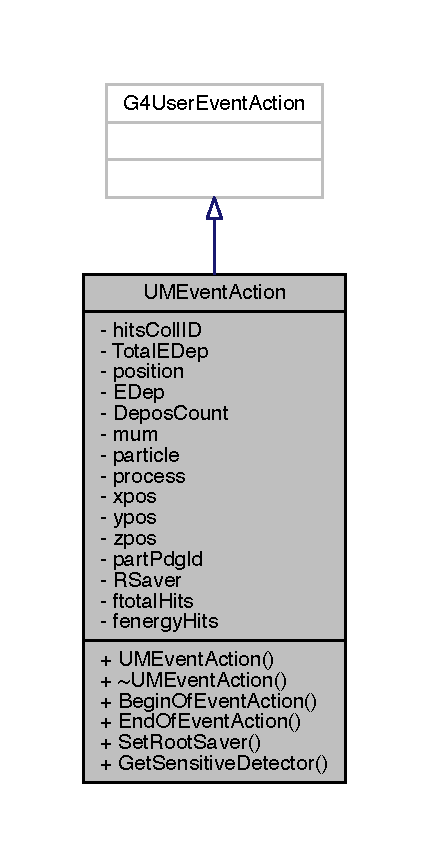
\includegraphics[width=206pt]{classUMEventAction__inherit__graph}
\end{center}
\end{figure}


Collaboration diagram for U\+M\+Event\+Action\+:
\nopagebreak
\begin{figure}[H]
\begin{center}
\leavevmode
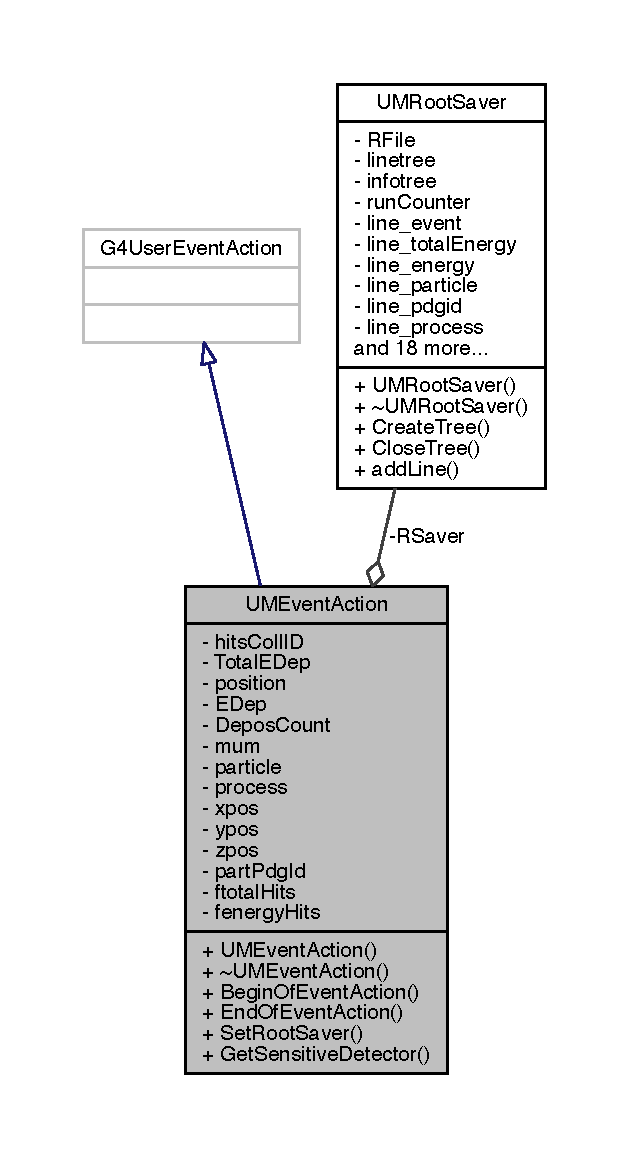
\includegraphics[height=550pt]{classUMEventAction__coll__graph}
\end{center}
\end{figure}
\subsection*{Public Member Functions}
\begin{DoxyCompactItemize}
\item 
\hyperlink{classUMEventAction_a81e4b6ebea6a9c34692964c08bd1a7c8}{U\+M\+Event\+Action} (ofstream \&total\+Hits, ofstream \&energy\+Hits)
\begin{DoxyCompactList}\small\item\em Constructor. \end{DoxyCompactList}\item 
\hyperlink{classUMEventAction_a503b6634cb64db87aea320d1c8810692}{$\sim$\+U\+M\+Event\+Action} ()
\begin{DoxyCompactList}\small\item\em Destructor. \end{DoxyCompactList}\item 
void \hyperlink{classUMEventAction_af1288b6bdbdfbe40a9fafc13b84250db}{Begin\+Of\+Event\+Action} (const G4\+Event $\ast$an\+Event)
\begin{DoxyCompactList}\small\item\em What happens at the beginning of Event? \end{DoxyCompactList}\item 
void \hyperlink{classUMEventAction_ab31f064263770cd6f2daeca58ac160ee}{End\+Of\+Event\+Action} (const G4\+Event $\ast$an\+Event)
\begin{DoxyCompactList}\small\item\em What happens at the end of an Event? \end{DoxyCompactList}\item 
void \hyperlink{classUMEventAction_a5f4b755e2e7b9c61ed355b6e21dd93e0}{Set\+Root\+Saver} (\hyperlink{classUMRootSaver}{U\+M\+Root\+Saver} $\ast$saver)
\begin{DoxyCompactList}\small\item\em Set up the R\+O\+O\+T saver. \end{DoxyCompactList}\item 
\hyperlink{classUMSD}{U\+M\+S\+D} $\ast$ \hyperlink{classUMEventAction_a8748655e8f5afe57a0c7ed6e83038ee0}{Get\+Sensitive\+Detector} (G4\+String detname)
\begin{DoxyCompactList}\small\item\em Get the sensitive detector. \end{DoxyCompactList}\end{DoxyCompactItemize}
\subsection*{Private Attributes}
\begin{DoxyCompactItemize}
\item 
G4int \hyperlink{classUMEventAction_a93249ca25c9565def0692d174a3e535e}{hits\+Coll\+I\+D}
\item 
G4double \hyperlink{classUMEventAction_a5a3fe12d0cc54f760499e76675044531}{Total\+E\+Dep}
\item 
G4\+Three\+Vector \hyperlink{classUMEventAction_aca4a227170c74e840a4ff2748efc20a2}{position}
\item 
G4double \hyperlink{classUMEventAction_a08ad731762fc90f81d56438383ee7bd8}{E\+Dep}
\item 
G4int \hyperlink{classUMEventAction_a55440e417cd0da1c627acb845a1108b9}{Depos\+Count}
\item 
G4int \hyperlink{classUMEventAction_a42d549a67c09ac22be18a0724b3f35ad}{mum}
\item 
G4\+String \hyperlink{classUMEventAction_a3bf2d2815501186c39a1985f47b2f5ab}{particle}
\item 
G4\+String \hyperlink{classUMEventAction_a2eabd29838c45226cc745aaeaee2a957}{process}
\item 
G4double \hyperlink{classUMEventAction_a006e73f519211d125c5f2ac070fbf489}{xpos}
\item 
G4double \hyperlink{classUMEventAction_a06f954b93a1ec5dc1e74dbd0f08fa258}{ypos}
\item 
G4double \hyperlink{classUMEventAction_a6a8137a0ba95725f0bcd80f9a433dcb0}{zpos}
\item 
G4int \hyperlink{classUMEventAction_a70cb8cc9f3d9820a85aedf4d245f5435}{part\+Pdg\+Id}
\item 
\hyperlink{classUMRootSaver}{U\+M\+Root\+Saver} $\ast$ \hyperlink{classUMEventAction_a1ad55dd713ab67a94b7989e09a7d19a9}{R\+Saver}
\item 
std\+::ofstream \& \hyperlink{classUMEventAction_a9bbd91659dd5720ff846cb231f8b8a81}{ftotal\+Hits}
\item 
std\+::ofstream \& \hyperlink{classUMEventAction_a0a8010739f4395ee799c2b7a106263b2}{fenergy\+Hits}
\end{DoxyCompactItemize}


\subsection{Constructor \& Destructor Documentation}
\hypertarget{classUMEventAction_a81e4b6ebea6a9c34692964c08bd1a7c8}{}\index{U\+M\+Event\+Action@{U\+M\+Event\+Action}!U\+M\+Event\+Action@{U\+M\+Event\+Action}}
\index{U\+M\+Event\+Action@{U\+M\+Event\+Action}!U\+M\+Event\+Action@{U\+M\+Event\+Action}}
\subsubsection[{U\+M\+Event\+Action(ofstream \&total\+Hits, ofstream \&energy\+Hits)}]{\setlength{\rightskip}{0pt plus 5cm}U\+M\+Event\+Action\+::\+U\+M\+Event\+Action (
\begin{DoxyParamCaption}
\item[{ofstream \&}]{total\+Hits, }
\item[{ofstream \&}]{energy\+Hits}
\end{DoxyParamCaption}
)}\label{classUMEventAction_a81e4b6ebea6a9c34692964c08bd1a7c8}


Constructor. 

\hypertarget{classUMEventAction_a503b6634cb64db87aea320d1c8810692}{}\index{U\+M\+Event\+Action@{U\+M\+Event\+Action}!````~U\+M\+Event\+Action@{$\sim$\+U\+M\+Event\+Action}}
\index{````~U\+M\+Event\+Action@{$\sim$\+U\+M\+Event\+Action}!U\+M\+Event\+Action@{U\+M\+Event\+Action}}
\subsubsection[{$\sim$\+U\+M\+Event\+Action()}]{\setlength{\rightskip}{0pt plus 5cm}U\+M\+Event\+Action\+::$\sim$\+U\+M\+Event\+Action (
\begin{DoxyParamCaption}
{}
\end{DoxyParamCaption}
)}\label{classUMEventAction_a503b6634cb64db87aea320d1c8810692}


Destructor. 

pass 

\subsection{Member Function Documentation}
\hypertarget{classUMEventAction_af1288b6bdbdfbe40a9fafc13b84250db}{}\index{U\+M\+Event\+Action@{U\+M\+Event\+Action}!Begin\+Of\+Event\+Action@{Begin\+Of\+Event\+Action}}
\index{Begin\+Of\+Event\+Action@{Begin\+Of\+Event\+Action}!U\+M\+Event\+Action@{U\+M\+Event\+Action}}
\subsubsection[{Begin\+Of\+Event\+Action(const G4\+Event $\ast$an\+Event)}]{\setlength{\rightskip}{0pt plus 5cm}void U\+M\+Event\+Action\+::\+Begin\+Of\+Event\+Action (
\begin{DoxyParamCaption}
\item[{const G4\+Event $\ast$}]{an\+Event}
\end{DoxyParamCaption}
)}\label{classUMEventAction_af1288b6bdbdfbe40a9fafc13b84250db}


What happens at the beginning of Event? 

At the begin of event setup the S\+D Manager and the hits Collection. \hypertarget{classUMEventAction_ab31f064263770cd6f2daeca58ac160ee}{}\index{U\+M\+Event\+Action@{U\+M\+Event\+Action}!End\+Of\+Event\+Action@{End\+Of\+Event\+Action}}
\index{End\+Of\+Event\+Action@{End\+Of\+Event\+Action}!U\+M\+Event\+Action@{U\+M\+Event\+Action}}
\subsubsection[{End\+Of\+Event\+Action(const G4\+Event $\ast$an\+Event)}]{\setlength{\rightskip}{0pt plus 5cm}void U\+M\+Event\+Action\+::\+End\+Of\+Event\+Action (
\begin{DoxyParamCaption}
\item[{const G4\+Event $\ast$}]{an\+Event}
\end{DoxyParamCaption}
)}\label{classUMEventAction_ab31f064263770cd6f2daeca58ac160ee}


What happens at the end of an Event? 

At the end of the event... loop over hits

Get the information from the hit

\begin{DoxyAttention}{Attention}
\{should be given in mm !!!\}
\end{DoxyAttention}
uncomment below to write non-\/serialised file line

to save up some storage save only if energy deposited within the drift gas volumn and if the energy is larger than 26e\+V = ionisation of Argon

\begin{DoxyAttention}{Attention}
\{position in um, energy in ke\+V\} 
\end{DoxyAttention}
\hypertarget{classUMEventAction_a8748655e8f5afe57a0c7ed6e83038ee0}{}\index{U\+M\+Event\+Action@{U\+M\+Event\+Action}!Get\+Sensitive\+Detector@{Get\+Sensitive\+Detector}}
\index{Get\+Sensitive\+Detector@{Get\+Sensitive\+Detector}!U\+M\+Event\+Action@{U\+M\+Event\+Action}}
\subsubsection[{Get\+Sensitive\+Detector(\+G4\+String detname)}]{\setlength{\rightskip}{0pt plus 5cm}{\bf U\+M\+S\+D} $\ast$ U\+M\+Event\+Action\+::\+Get\+Sensitive\+Detector (
\begin{DoxyParamCaption}
\item[{G4\+String}]{detname}
\end{DoxyParamCaption}
)}\label{classUMEventAction_a8748655e8f5afe57a0c7ed6e83038ee0}


Get the sensitive detector. 

Get the Sensitive Detector. \hypertarget{classUMEventAction_a5f4b755e2e7b9c61ed355b6e21dd93e0}{}\index{U\+M\+Event\+Action@{U\+M\+Event\+Action}!Set\+Root\+Saver@{Set\+Root\+Saver}}
\index{Set\+Root\+Saver@{Set\+Root\+Saver}!U\+M\+Event\+Action@{U\+M\+Event\+Action}}
\subsubsection[{Set\+Root\+Saver(\+U\+M\+Root\+Saver $\ast$saver)}]{\setlength{\rightskip}{0pt plus 5cm}void U\+M\+Event\+Action\+::\+Set\+Root\+Saver (
\begin{DoxyParamCaption}
\item[{{\bf U\+M\+Root\+Saver} $\ast$}]{saver}
\end{DoxyParamCaption}
)\hspace{0.3cm}{\ttfamily [inline]}}\label{classUMEventAction_a5f4b755e2e7b9c61ed355b6e21dd93e0}


Set up the R\+O\+O\+T saver. 



\subsection{Field Documentation}
\hypertarget{classUMEventAction_a55440e417cd0da1c627acb845a1108b9}{}\index{U\+M\+Event\+Action@{U\+M\+Event\+Action}!Depos\+Count@{Depos\+Count}}
\index{Depos\+Count@{Depos\+Count}!U\+M\+Event\+Action@{U\+M\+Event\+Action}}
\subsubsection[{Depos\+Count}]{\setlength{\rightskip}{0pt plus 5cm}G4int U\+M\+Event\+Action\+::\+Depos\+Count\hspace{0.3cm}{\ttfamily [private]}}\label{classUMEventAction_a55440e417cd0da1c627acb845a1108b9}
\hypertarget{classUMEventAction_a08ad731762fc90f81d56438383ee7bd8}{}\index{U\+M\+Event\+Action@{U\+M\+Event\+Action}!E\+Dep@{E\+Dep}}
\index{E\+Dep@{E\+Dep}!U\+M\+Event\+Action@{U\+M\+Event\+Action}}
\subsubsection[{E\+Dep}]{\setlength{\rightskip}{0pt plus 5cm}G4double U\+M\+Event\+Action\+::\+E\+Dep\hspace{0.3cm}{\ttfamily [private]}}\label{classUMEventAction_a08ad731762fc90f81d56438383ee7bd8}
\hypertarget{classUMEventAction_a0a8010739f4395ee799c2b7a106263b2}{}\index{U\+M\+Event\+Action@{U\+M\+Event\+Action}!fenergy\+Hits@{fenergy\+Hits}}
\index{fenergy\+Hits@{fenergy\+Hits}!U\+M\+Event\+Action@{U\+M\+Event\+Action}}
\subsubsection[{fenergy\+Hits}]{\setlength{\rightskip}{0pt plus 5cm}std\+::ofstream\& U\+M\+Event\+Action\+::fenergy\+Hits\hspace{0.3cm}{\ttfamily [private]}}\label{classUMEventAction_a0a8010739f4395ee799c2b7a106263b2}
\hypertarget{classUMEventAction_a9bbd91659dd5720ff846cb231f8b8a81}{}\index{U\+M\+Event\+Action@{U\+M\+Event\+Action}!ftotal\+Hits@{ftotal\+Hits}}
\index{ftotal\+Hits@{ftotal\+Hits}!U\+M\+Event\+Action@{U\+M\+Event\+Action}}
\subsubsection[{ftotal\+Hits}]{\setlength{\rightskip}{0pt plus 5cm}std\+::ofstream\& U\+M\+Event\+Action\+::ftotal\+Hits\hspace{0.3cm}{\ttfamily [private]}}\label{classUMEventAction_a9bbd91659dd5720ff846cb231f8b8a81}
\hypertarget{classUMEventAction_a93249ca25c9565def0692d174a3e535e}{}\index{U\+M\+Event\+Action@{U\+M\+Event\+Action}!hits\+Coll\+I\+D@{hits\+Coll\+I\+D}}
\index{hits\+Coll\+I\+D@{hits\+Coll\+I\+D}!U\+M\+Event\+Action@{U\+M\+Event\+Action}}
\subsubsection[{hits\+Coll\+I\+D}]{\setlength{\rightskip}{0pt plus 5cm}G4int U\+M\+Event\+Action\+::hits\+Coll\+I\+D\hspace{0.3cm}{\ttfamily [private]}}\label{classUMEventAction_a93249ca25c9565def0692d174a3e535e}
\hypertarget{classUMEventAction_a42d549a67c09ac22be18a0724b3f35ad}{}\index{U\+M\+Event\+Action@{U\+M\+Event\+Action}!mum@{mum}}
\index{mum@{mum}!U\+M\+Event\+Action@{U\+M\+Event\+Action}}
\subsubsection[{mum}]{\setlength{\rightskip}{0pt plus 5cm}G4int U\+M\+Event\+Action\+::mum\hspace{0.3cm}{\ttfamily [private]}}\label{classUMEventAction_a42d549a67c09ac22be18a0724b3f35ad}
\hypertarget{classUMEventAction_a3bf2d2815501186c39a1985f47b2f5ab}{}\index{U\+M\+Event\+Action@{U\+M\+Event\+Action}!particle@{particle}}
\index{particle@{particle}!U\+M\+Event\+Action@{U\+M\+Event\+Action}}
\subsubsection[{particle}]{\setlength{\rightskip}{0pt plus 5cm}G4\+String U\+M\+Event\+Action\+::particle\hspace{0.3cm}{\ttfamily [private]}}\label{classUMEventAction_a3bf2d2815501186c39a1985f47b2f5ab}
\hypertarget{classUMEventAction_a70cb8cc9f3d9820a85aedf4d245f5435}{}\index{U\+M\+Event\+Action@{U\+M\+Event\+Action}!part\+Pdg\+Id@{part\+Pdg\+Id}}
\index{part\+Pdg\+Id@{part\+Pdg\+Id}!U\+M\+Event\+Action@{U\+M\+Event\+Action}}
\subsubsection[{part\+Pdg\+Id}]{\setlength{\rightskip}{0pt plus 5cm}G4int U\+M\+Event\+Action\+::part\+Pdg\+Id\hspace{0.3cm}{\ttfamily [private]}}\label{classUMEventAction_a70cb8cc9f3d9820a85aedf4d245f5435}
\hypertarget{classUMEventAction_aca4a227170c74e840a4ff2748efc20a2}{}\index{U\+M\+Event\+Action@{U\+M\+Event\+Action}!position@{position}}
\index{position@{position}!U\+M\+Event\+Action@{U\+M\+Event\+Action}}
\subsubsection[{position}]{\setlength{\rightskip}{0pt plus 5cm}G4\+Three\+Vector U\+M\+Event\+Action\+::position\hspace{0.3cm}{\ttfamily [private]}}\label{classUMEventAction_aca4a227170c74e840a4ff2748efc20a2}
\hypertarget{classUMEventAction_a2eabd29838c45226cc745aaeaee2a957}{}\index{U\+M\+Event\+Action@{U\+M\+Event\+Action}!process@{process}}
\index{process@{process}!U\+M\+Event\+Action@{U\+M\+Event\+Action}}
\subsubsection[{process}]{\setlength{\rightskip}{0pt plus 5cm}G4\+String U\+M\+Event\+Action\+::process\hspace{0.3cm}{\ttfamily [private]}}\label{classUMEventAction_a2eabd29838c45226cc745aaeaee2a957}
\hypertarget{classUMEventAction_a1ad55dd713ab67a94b7989e09a7d19a9}{}\index{U\+M\+Event\+Action@{U\+M\+Event\+Action}!R\+Saver@{R\+Saver}}
\index{R\+Saver@{R\+Saver}!U\+M\+Event\+Action@{U\+M\+Event\+Action}}
\subsubsection[{R\+Saver}]{\setlength{\rightskip}{0pt plus 5cm}{\bf U\+M\+Root\+Saver}$\ast$ U\+M\+Event\+Action\+::\+R\+Saver\hspace{0.3cm}{\ttfamily [private]}}\label{classUMEventAction_a1ad55dd713ab67a94b7989e09a7d19a9}
\hypertarget{classUMEventAction_a5a3fe12d0cc54f760499e76675044531}{}\index{U\+M\+Event\+Action@{U\+M\+Event\+Action}!Total\+E\+Dep@{Total\+E\+Dep}}
\index{Total\+E\+Dep@{Total\+E\+Dep}!U\+M\+Event\+Action@{U\+M\+Event\+Action}}
\subsubsection[{Total\+E\+Dep}]{\setlength{\rightskip}{0pt plus 5cm}G4double U\+M\+Event\+Action\+::\+Total\+E\+Dep\hspace{0.3cm}{\ttfamily [private]}}\label{classUMEventAction_a5a3fe12d0cc54f760499e76675044531}
\hypertarget{classUMEventAction_a006e73f519211d125c5f2ac070fbf489}{}\index{U\+M\+Event\+Action@{U\+M\+Event\+Action}!xpos@{xpos}}
\index{xpos@{xpos}!U\+M\+Event\+Action@{U\+M\+Event\+Action}}
\subsubsection[{xpos}]{\setlength{\rightskip}{0pt plus 5cm}G4double U\+M\+Event\+Action\+::xpos\hspace{0.3cm}{\ttfamily [private]}}\label{classUMEventAction_a006e73f519211d125c5f2ac070fbf489}
\hypertarget{classUMEventAction_a06f954b93a1ec5dc1e74dbd0f08fa258}{}\index{U\+M\+Event\+Action@{U\+M\+Event\+Action}!ypos@{ypos}}
\index{ypos@{ypos}!U\+M\+Event\+Action@{U\+M\+Event\+Action}}
\subsubsection[{ypos}]{\setlength{\rightskip}{0pt plus 5cm}G4double U\+M\+Event\+Action\+::ypos\hspace{0.3cm}{\ttfamily [private]}}\label{classUMEventAction_a06f954b93a1ec5dc1e74dbd0f08fa258}
\hypertarget{classUMEventAction_a6a8137a0ba95725f0bcd80f9a433dcb0}{}\index{U\+M\+Event\+Action@{U\+M\+Event\+Action}!zpos@{zpos}}
\index{zpos@{zpos}!U\+M\+Event\+Action@{U\+M\+Event\+Action}}
\subsubsection[{zpos}]{\setlength{\rightskip}{0pt plus 5cm}G4double U\+M\+Event\+Action\+::zpos\hspace{0.3cm}{\ttfamily [private]}}\label{classUMEventAction_a6a8137a0ba95725f0bcd80f9a433dcb0}


The documentation for this class was generated from the following files\+:\begin{DoxyCompactItemize}
\item 
include/\hyperlink{UMEventAction_8hh}{U\+M\+Event\+Action.\+hh}\item 
src/\hyperlink{UMEventAction_8cc}{U\+M\+Event\+Action.\+cc}\end{DoxyCompactItemize}

\hypertarget{classUMHit}{}\section{U\+M\+Hit Class Reference}
\label{classUMHit}\index{U\+M\+Hit@{U\+M\+Hit}}


{\ttfamily \#include $<$U\+M\+Hit.\+hh$>$}



Inheritance diagram for U\+M\+Hit\+:
\nopagebreak
\begin{figure}[H]
\begin{center}
\leavevmode
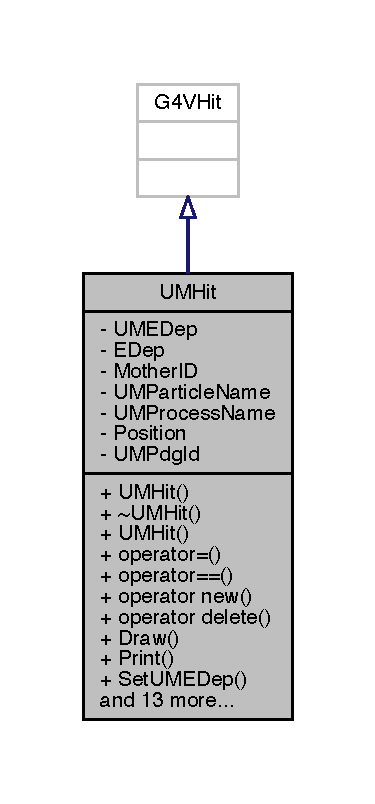
\includegraphics[width=180pt]{classUMHit__inherit__graph}
\end{center}
\end{figure}


Collaboration diagram for U\+M\+Hit\+:
\nopagebreak
\begin{figure}[H]
\begin{center}
\leavevmode
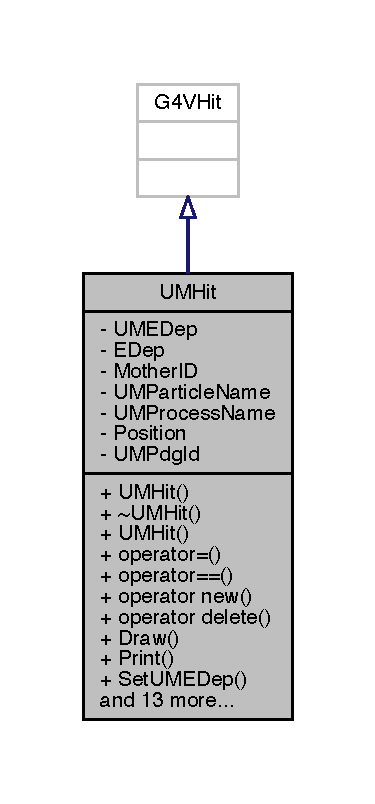
\includegraphics[width=180pt]{classUMHit__coll__graph}
\end{center}
\end{figure}
\subsection*{Public Member Functions}
\begin{DoxyCompactItemize}
\item 
\hyperlink{classUMHit_a394e817a3a89fab49c06d00fda476050}{U\+M\+Hit} ()
\begin{DoxyCompactList}\small\item\em Constructor and set the deposited energy to 0. \end{DoxyCompactList}\item 
\hyperlink{classUMHit_a1baa8f810beaa912147438a9551b59e8}{$\sim$\+U\+M\+Hit} ()
\begin{DoxyCompactList}\small\item\em Destructor -\/ None. \end{DoxyCompactList}\item 
\hyperlink{classUMHit_aca5680bf533cac7ff218317ddbdac93b}{U\+M\+Hit} (const \hyperlink{classUMHit}{U\+M\+Hit} \&right)
\begin{DoxyCompactList}\small\item\em Constructor. \end{DoxyCompactList}\item 
const \hyperlink{classUMHit}{U\+M\+Hit} \& \hyperlink{classUMHit_a2c5c0ca780f8089def10974f044c2111}{operator=} (const \hyperlink{classUMHit}{U\+M\+Hit} \&right)
\begin{DoxyCompactList}\small\item\em Define = hit operator. \end{DoxyCompactList}\item 
G4bool \hyperlink{classUMHit_af502a147d6cb493e5bacfde7019b1d0d}{operator==} (const \hyperlink{classUMHit}{U\+M\+Hit} \&right) const 
\begin{DoxyCompactList}\small\item\em Define == hit operator. \end{DoxyCompactList}\item 
void $\ast$ \hyperlink{classUMHit_a9ea7dddc4dd813d59f321443f653815d}{operator new} (size\+\_\+t)
\item 
void \hyperlink{classUMHit_a472a42be272e3bf0e2e01889051c0b42}{operator delete} (void $\ast$hit)
\item 
virtual void \hyperlink{classUMHit_ae0fb0c79824f713956c36d83ff8b2685}{Draw} ()
\item 
virtual void \hyperlink{classUMHit_ac06e6339f2a24ab539bb0b811bf85e8d}{Print} ()
\item 
void \hyperlink{classUMHit_af0222028e4ccfb5aa14ea5956ab8e6b7}{Set\+U\+M\+E\+Dep} (const G4double e)
\begin{DoxyCompactList}\small\item\em Setter for Energy Deposit. \end{DoxyCompactList}\item 
G4double \hyperlink{classUMHit_a972fd7fa5472ed40803bc78f90177c74}{Get\+U\+M\+E\+Dep} () const 
\item 
void \hyperlink{classUMHit_a782a87ef10c335a5e3046cb096f183f1}{Set\+Position} (const G4\+Three\+Vector xyz)
\begin{DoxyCompactList}\small\item\em Setter for Position. \end{DoxyCompactList}\item 
G4\+Three\+Vector \hyperlink{classUMHit_ad4fa003468a310edb749395e3dbb78c1}{Get\+Pos} () const 
\begin{DoxyCompactList}\small\item\em Getter for position. \end{DoxyCompactList}\item 
void \hyperlink{classUMHit_a1f872ac3231beb480095f417085d9205}{Set\+U\+M\+Particle\+Name} (const G4\+String pn)
\begin{DoxyCompactList}\small\item\em Setter for Particle Name. \end{DoxyCompactList}\item 
void \hyperlink{classUMHit_af922d50470b941d27f60668242885784}{Set\+U\+M\+Process\+Name} (const G4\+String pn)
\begin{DoxyCompactList}\small\item\em Setter for Process Name. \end{DoxyCompactList}\item 
G4\+String \hyperlink{classUMHit_ae91e909b64f2059f37b1068b594a25c6}{Get\+U\+M\+Particle\+Name} () const 
\begin{DoxyCompactList}\small\item\em Getter for Process Name. \end{DoxyCompactList}\item 
G4\+String \hyperlink{classUMHit_ade4194ef36b9553b403c60d31f031fdf}{Get\+U\+M\+Process\+Name} () const 
\begin{DoxyCompactList}\small\item\em Getter for process name. \end{DoxyCompactList}\item 
void \hyperlink{classUMHit_aa42edfe14f74310860d159eb4274a53c}{Set\+Mother\+I\+D} (const G4int M\+I\+D)
\begin{DoxyCompactList}\small\item\em Setter for mother particle. \end{DoxyCompactList}\item 
G4int \hyperlink{classUMHit_af9e683061a4dae1139102374b5a83283}{Get\+Mother\+I\+D} () const 
\begin{DoxyCompactList}\small\item\em Getter for mother particle. \end{DoxyCompactList}\item 
G4int \hyperlink{classUMHit_ad4c59e6ba7a5a0bc68d36d8b75f3b6c0}{Get\+U\+M\+Pdg\+Id} () const 
\begin{DoxyCompactList}\small\item\em Getter for pdg I\+D. \end{DoxyCompactList}\item 
void \hyperlink{classUMHit_a57b8887426a1eb3f888025c2408596f6}{Set\+U\+M\+Pdg\+Id} (const G4int pdgid)
\begin{DoxyCompactList}\small\item\em Setter for pdf I\+D. \end{DoxyCompactList}\item 
void \hyperlink{classUMHit_ad8f0847257537f21f4758459f5fa3dbd}{Add\+E\+Dep} (const double e)
\begin{DoxyCompactList}\small\item\em Adding deposited energy to total deposited energy. \end{DoxyCompactList}\item 
G4double \hyperlink{classUMHit_a1196b569b6874732e58dabb8ef49a567}{Get\+E\+Dep} () const 
\begin{DoxyCompactList}\small\item\em Getter for deposited energy. \end{DoxyCompactList}\end{DoxyCompactItemize}
\subsection*{Private Attributes}
\begin{DoxyCompactItemize}
\item 
G4double \hyperlink{classUMHit_aec0cf8d46f391050ad456c3713da6ba0}{U\+M\+E\+Dep}
\item 
G4double \hyperlink{classUMHit_a69d9bbb76e36dfececf0cbfc0f2f4f4b}{E\+Dep}
\item 
G4int \hyperlink{classUMHit_a62d959b08653e6d345dabdbc03a4305c}{Mother\+I\+D}
\item 
G4\+String \hyperlink{classUMHit_a7889f1c0495ffeb5cfe5cccd57d98f92}{U\+M\+Particle\+Name}
\item 
G4\+String \hyperlink{classUMHit_ac4f5fd214eb213afa3560a18d9b6120b}{U\+M\+Process\+Name}
\item 
G4\+Three\+Vector \hyperlink{classUMHit_a89b65132e5a6168e2f7e0fa93b8fd677}{Position}
\item 
G4int \hyperlink{classUMHit_a014c9504d8aed42c0eba0cf2a24c2713}{U\+M\+Pdg\+Id}
\end{DoxyCompactItemize}


\subsection{Detailed Description}
Header for Hit definition for the S\+D

\begin{DoxyAuthor}{Author}
Nikolaos Karastathis $<$ nkarast .at. cern .dot. ch $>$ 
\end{DoxyAuthor}
\begin{DoxyVersion}{Version}
v2.\+0 
\end{DoxyVersion}


\subsection{Constructor \& Destructor Documentation}
\hypertarget{classUMHit_a394e817a3a89fab49c06d00fda476050}{}\index{U\+M\+Hit@{U\+M\+Hit}!U\+M\+Hit@{U\+M\+Hit}}
\index{U\+M\+Hit@{U\+M\+Hit}!U\+M\+Hit@{U\+M\+Hit}}
\subsubsection[{U\+M\+Hit()}]{\setlength{\rightskip}{0pt plus 5cm}U\+M\+Hit\+::\+U\+M\+Hit (
\begin{DoxyParamCaption}
{}
\end{DoxyParamCaption}
)\hspace{0.3cm}{\ttfamily [inline]}}\label{classUMHit_a394e817a3a89fab49c06d00fda476050}


Constructor and set the deposited energy to 0. 

\hypertarget{classUMHit_a1baa8f810beaa912147438a9551b59e8}{}\index{U\+M\+Hit@{U\+M\+Hit}!````~U\+M\+Hit@{$\sim$\+U\+M\+Hit}}
\index{````~U\+M\+Hit@{$\sim$\+U\+M\+Hit}!U\+M\+Hit@{U\+M\+Hit}}
\subsubsection[{$\sim$\+U\+M\+Hit()}]{\setlength{\rightskip}{0pt plus 5cm}U\+M\+Hit\+::$\sim$\+U\+M\+Hit (
\begin{DoxyParamCaption}
{}
\end{DoxyParamCaption}
)\hspace{0.3cm}{\ttfamily [inline]}}\label{classUMHit_a1baa8f810beaa912147438a9551b59e8}


Destructor -\/ None. 

\hypertarget{classUMHit_aca5680bf533cac7ff218317ddbdac93b}{}\index{U\+M\+Hit@{U\+M\+Hit}!U\+M\+Hit@{U\+M\+Hit}}
\index{U\+M\+Hit@{U\+M\+Hit}!U\+M\+Hit@{U\+M\+Hit}}
\subsubsection[{U\+M\+Hit(const U\+M\+Hit \&right)}]{\setlength{\rightskip}{0pt plus 5cm}U\+M\+Hit\+::\+U\+M\+Hit (
\begin{DoxyParamCaption}
\item[{const {\bf U\+M\+Hit} \&}]{right}
\end{DoxyParamCaption}
)}\label{classUMHit_aca5680bf533cac7ff218317ddbdac93b}


Constructor. 



\subsection{Member Function Documentation}
\hypertarget{classUMHit_ad8f0847257537f21f4758459f5fa3dbd}{}\index{U\+M\+Hit@{U\+M\+Hit}!Add\+E\+Dep@{Add\+E\+Dep}}
\index{Add\+E\+Dep@{Add\+E\+Dep}!U\+M\+Hit@{U\+M\+Hit}}
\subsubsection[{Add\+E\+Dep(const double e)}]{\setlength{\rightskip}{0pt plus 5cm}void U\+M\+Hit\+::\+Add\+E\+Dep (
\begin{DoxyParamCaption}
\item[{const double}]{e}
\end{DoxyParamCaption}
)\hspace{0.3cm}{\ttfamily [inline]}}\label{classUMHit_ad8f0847257537f21f4758459f5fa3dbd}


Adding deposited energy to total deposited energy. 

\hypertarget{classUMHit_ae0fb0c79824f713956c36d83ff8b2685}{}\index{U\+M\+Hit@{U\+M\+Hit}!Draw@{Draw}}
\index{Draw@{Draw}!U\+M\+Hit@{U\+M\+Hit}}
\subsubsection[{Draw()}]{\setlength{\rightskip}{0pt plus 5cm}void U\+M\+Hit\+::\+Draw (
\begin{DoxyParamCaption}
{}
\end{DoxyParamCaption}
)\hspace{0.3cm}{\ttfamily [virtual]}}\label{classUMHit_ae0fb0c79824f713956c36d83ff8b2685}
pass \hypertarget{classUMHit_a1196b569b6874732e58dabb8ef49a567}{}\index{U\+M\+Hit@{U\+M\+Hit}!Get\+E\+Dep@{Get\+E\+Dep}}
\index{Get\+E\+Dep@{Get\+E\+Dep}!U\+M\+Hit@{U\+M\+Hit}}
\subsubsection[{Get\+E\+Dep() const }]{\setlength{\rightskip}{0pt plus 5cm}G4double U\+M\+Hit\+::\+Get\+E\+Dep (
\begin{DoxyParamCaption}
{}
\end{DoxyParamCaption}
) const\hspace{0.3cm}{\ttfamily [inline]}}\label{classUMHit_a1196b569b6874732e58dabb8ef49a567}


Getter for deposited energy. 

\hypertarget{classUMHit_af9e683061a4dae1139102374b5a83283}{}\index{U\+M\+Hit@{U\+M\+Hit}!Get\+Mother\+I\+D@{Get\+Mother\+I\+D}}
\index{Get\+Mother\+I\+D@{Get\+Mother\+I\+D}!U\+M\+Hit@{U\+M\+Hit}}
\subsubsection[{Get\+Mother\+I\+D() const }]{\setlength{\rightskip}{0pt plus 5cm}G4int U\+M\+Hit\+::\+Get\+Mother\+I\+D (
\begin{DoxyParamCaption}
{}
\end{DoxyParamCaption}
) const\hspace{0.3cm}{\ttfamily [inline]}}\label{classUMHit_af9e683061a4dae1139102374b5a83283}


Getter for mother particle. 

\hypertarget{classUMHit_ad4fa003468a310edb749395e3dbb78c1}{}\index{U\+M\+Hit@{U\+M\+Hit}!Get\+Pos@{Get\+Pos}}
\index{Get\+Pos@{Get\+Pos}!U\+M\+Hit@{U\+M\+Hit}}
\subsubsection[{Get\+Pos() const }]{\setlength{\rightskip}{0pt plus 5cm}G4\+Three\+Vector U\+M\+Hit\+::\+Get\+Pos (
\begin{DoxyParamCaption}
{}
\end{DoxyParamCaption}
) const\hspace{0.3cm}{\ttfamily [inline]}}\label{classUMHit_ad4fa003468a310edb749395e3dbb78c1}


Getter for position. 

\hypertarget{classUMHit_a972fd7fa5472ed40803bc78f90177c74}{}\index{U\+M\+Hit@{U\+M\+Hit}!Get\+U\+M\+E\+Dep@{Get\+U\+M\+E\+Dep}}
\index{Get\+U\+M\+E\+Dep@{Get\+U\+M\+E\+Dep}!U\+M\+Hit@{U\+M\+Hit}}
\subsubsection[{Get\+U\+M\+E\+Dep() const }]{\setlength{\rightskip}{0pt plus 5cm}G4double U\+M\+Hit\+::\+Get\+U\+M\+E\+Dep (
\begin{DoxyParamCaption}
{}
\end{DoxyParamCaption}
) const\hspace{0.3cm}{\ttfamily [inline]}}\label{classUMHit_a972fd7fa5472ed40803bc78f90177c74}
\hypertarget{classUMHit_ae91e909b64f2059f37b1068b594a25c6}{}\index{U\+M\+Hit@{U\+M\+Hit}!Get\+U\+M\+Particle\+Name@{Get\+U\+M\+Particle\+Name}}
\index{Get\+U\+M\+Particle\+Name@{Get\+U\+M\+Particle\+Name}!U\+M\+Hit@{U\+M\+Hit}}
\subsubsection[{Get\+U\+M\+Particle\+Name() const }]{\setlength{\rightskip}{0pt plus 5cm}G4\+String U\+M\+Hit\+::\+Get\+U\+M\+Particle\+Name (
\begin{DoxyParamCaption}
{}
\end{DoxyParamCaption}
) const\hspace{0.3cm}{\ttfamily [inline]}}\label{classUMHit_ae91e909b64f2059f37b1068b594a25c6}


Getter for Process Name. 

\hypertarget{classUMHit_ad4c59e6ba7a5a0bc68d36d8b75f3b6c0}{}\index{U\+M\+Hit@{U\+M\+Hit}!Get\+U\+M\+Pdg\+Id@{Get\+U\+M\+Pdg\+Id}}
\index{Get\+U\+M\+Pdg\+Id@{Get\+U\+M\+Pdg\+Id}!U\+M\+Hit@{U\+M\+Hit}}
\subsubsection[{Get\+U\+M\+Pdg\+Id() const }]{\setlength{\rightskip}{0pt plus 5cm}G4int U\+M\+Hit\+::\+Get\+U\+M\+Pdg\+Id (
\begin{DoxyParamCaption}
{}
\end{DoxyParamCaption}
) const\hspace{0.3cm}{\ttfamily [inline]}}\label{classUMHit_ad4c59e6ba7a5a0bc68d36d8b75f3b6c0}


Getter for pdg I\+D. 

\hypertarget{classUMHit_ade4194ef36b9553b403c60d31f031fdf}{}\index{U\+M\+Hit@{U\+M\+Hit}!Get\+U\+M\+Process\+Name@{Get\+U\+M\+Process\+Name}}
\index{Get\+U\+M\+Process\+Name@{Get\+U\+M\+Process\+Name}!U\+M\+Hit@{U\+M\+Hit}}
\subsubsection[{Get\+U\+M\+Process\+Name() const }]{\setlength{\rightskip}{0pt plus 5cm}G4\+String U\+M\+Hit\+::\+Get\+U\+M\+Process\+Name (
\begin{DoxyParamCaption}
{}
\end{DoxyParamCaption}
) const\hspace{0.3cm}{\ttfamily [inline]}}\label{classUMHit_ade4194ef36b9553b403c60d31f031fdf}


Getter for process name. 

\hypertarget{classUMHit_a472a42be272e3bf0e2e01889051c0b42}{}\index{U\+M\+Hit@{U\+M\+Hit}!operator delete@{operator delete}}
\index{operator delete@{operator delete}!U\+M\+Hit@{U\+M\+Hit}}
\subsubsection[{operator delete(void $\ast$hit)}]{\setlength{\rightskip}{0pt plus 5cm}void U\+M\+Hit\+::operator delete (
\begin{DoxyParamCaption}
\item[{void $\ast$}]{hit}
\end{DoxyParamCaption}
)\hspace{0.3cm}{\ttfamily [inline]}}\label{classUMHit_a472a42be272e3bf0e2e01889051c0b42}
\hypertarget{classUMHit_a9ea7dddc4dd813d59f321443f653815d}{}\index{U\+M\+Hit@{U\+M\+Hit}!operator new@{operator new}}
\index{operator new@{operator new}!U\+M\+Hit@{U\+M\+Hit}}
\subsubsection[{operator new(size\+\_\+t)}]{\setlength{\rightskip}{0pt plus 5cm}void $\ast$ U\+M\+Hit\+::operator new (
\begin{DoxyParamCaption}
\item[{size\+\_\+t}]{}
\end{DoxyParamCaption}
)\hspace{0.3cm}{\ttfamily [inline]}}\label{classUMHit_a9ea7dddc4dd813d59f321443f653815d}
\hypertarget{classUMHit_a2c5c0ca780f8089def10974f044c2111}{}\index{U\+M\+Hit@{U\+M\+Hit}!operator=@{operator=}}
\index{operator=@{operator=}!U\+M\+Hit@{U\+M\+Hit}}
\subsubsection[{operator=(const U\+M\+Hit \&right)}]{\setlength{\rightskip}{0pt plus 5cm}const {\bf U\+M\+Hit} \& U\+M\+Hit\+::operator= (
\begin{DoxyParamCaption}
\item[{const {\bf U\+M\+Hit} \&}]{right}
\end{DoxyParamCaption}
)}\label{classUMHit_a2c5c0ca780f8089def10974f044c2111}


Define = hit operator. 

\hypertarget{classUMHit_af502a147d6cb493e5bacfde7019b1d0d}{}\index{U\+M\+Hit@{U\+M\+Hit}!operator==@{operator==}}
\index{operator==@{operator==}!U\+M\+Hit@{U\+M\+Hit}}
\subsubsection[{operator==(const U\+M\+Hit \&right) const }]{\setlength{\rightskip}{0pt plus 5cm}G4bool U\+M\+Hit\+::operator== (
\begin{DoxyParamCaption}
\item[{const {\bf U\+M\+Hit} \&}]{right}
\end{DoxyParamCaption}
) const}\label{classUMHit_af502a147d6cb493e5bacfde7019b1d0d}


Define == hit operator. 

\hypertarget{classUMHit_ac06e6339f2a24ab539bb0b811bf85e8d}{}\index{U\+M\+Hit@{U\+M\+Hit}!Print@{Print}}
\index{Print@{Print}!U\+M\+Hit@{U\+M\+Hit}}
\subsubsection[{Print()}]{\setlength{\rightskip}{0pt plus 5cm}void U\+M\+Hit\+::\+Print (
\begin{DoxyParamCaption}
{}
\end{DoxyParamCaption}
)\hspace{0.3cm}{\ttfamily [virtual]}}\label{classUMHit_ac06e6339f2a24ab539bb0b811bf85e8d}
std\+::ofstream fout(\char`\"{}hits.\+out\char`\"{},ios\+::app); fout $<$$<$ std\+::setw(10) $<$$<$ U\+M\+E\+Dep $<$$<$ \textquotesingle{}\textquotesingle{} $<$$<$ std\+::setw(20) $<$$<$ G4\+Best\+Unit(Position, \char`\"{}\+Length\char`\"{}) $<$$<$ \char`\"{}\textbackslash{}n\char`\"{}; \hypertarget{classUMHit_aa42edfe14f74310860d159eb4274a53c}{}\index{U\+M\+Hit@{U\+M\+Hit}!Set\+Mother\+I\+D@{Set\+Mother\+I\+D}}
\index{Set\+Mother\+I\+D@{Set\+Mother\+I\+D}!U\+M\+Hit@{U\+M\+Hit}}
\subsubsection[{Set\+Mother\+I\+D(const G4int M\+I\+D)}]{\setlength{\rightskip}{0pt plus 5cm}void U\+M\+Hit\+::\+Set\+Mother\+I\+D (
\begin{DoxyParamCaption}
\item[{const G4int}]{M\+I\+D}
\end{DoxyParamCaption}
)\hspace{0.3cm}{\ttfamily [inline]}}\label{classUMHit_aa42edfe14f74310860d159eb4274a53c}


Setter for mother particle. 

\hypertarget{classUMHit_a782a87ef10c335a5e3046cb096f183f1}{}\index{U\+M\+Hit@{U\+M\+Hit}!Set\+Position@{Set\+Position}}
\index{Set\+Position@{Set\+Position}!U\+M\+Hit@{U\+M\+Hit}}
\subsubsection[{Set\+Position(const G4\+Three\+Vector xyz)}]{\setlength{\rightskip}{0pt plus 5cm}void U\+M\+Hit\+::\+Set\+Position (
\begin{DoxyParamCaption}
\item[{const G4\+Three\+Vector}]{xyz}
\end{DoxyParamCaption}
)\hspace{0.3cm}{\ttfamily [inline]}}\label{classUMHit_a782a87ef10c335a5e3046cb096f183f1}


Setter for Position. 

\hypertarget{classUMHit_af0222028e4ccfb5aa14ea5956ab8e6b7}{}\index{U\+M\+Hit@{U\+M\+Hit}!Set\+U\+M\+E\+Dep@{Set\+U\+M\+E\+Dep}}
\index{Set\+U\+M\+E\+Dep@{Set\+U\+M\+E\+Dep}!U\+M\+Hit@{U\+M\+Hit}}
\subsubsection[{Set\+U\+M\+E\+Dep(const G4double e)}]{\setlength{\rightskip}{0pt plus 5cm}void U\+M\+Hit\+::\+Set\+U\+M\+E\+Dep (
\begin{DoxyParamCaption}
\item[{const G4double}]{e}
\end{DoxyParamCaption}
)\hspace{0.3cm}{\ttfamily [inline]}}\label{classUMHit_af0222028e4ccfb5aa14ea5956ab8e6b7}


Setter for Energy Deposit. 

\hypertarget{classUMHit_a1f872ac3231beb480095f417085d9205}{}\index{U\+M\+Hit@{U\+M\+Hit}!Set\+U\+M\+Particle\+Name@{Set\+U\+M\+Particle\+Name}}
\index{Set\+U\+M\+Particle\+Name@{Set\+U\+M\+Particle\+Name}!U\+M\+Hit@{U\+M\+Hit}}
\subsubsection[{Set\+U\+M\+Particle\+Name(const G4\+String pn)}]{\setlength{\rightskip}{0pt plus 5cm}void U\+M\+Hit\+::\+Set\+U\+M\+Particle\+Name (
\begin{DoxyParamCaption}
\item[{const G4\+String}]{pn}
\end{DoxyParamCaption}
)\hspace{0.3cm}{\ttfamily [inline]}}\label{classUMHit_a1f872ac3231beb480095f417085d9205}


Setter for Particle Name. 

\hypertarget{classUMHit_a57b8887426a1eb3f888025c2408596f6}{}\index{U\+M\+Hit@{U\+M\+Hit}!Set\+U\+M\+Pdg\+Id@{Set\+U\+M\+Pdg\+Id}}
\index{Set\+U\+M\+Pdg\+Id@{Set\+U\+M\+Pdg\+Id}!U\+M\+Hit@{U\+M\+Hit}}
\subsubsection[{Set\+U\+M\+Pdg\+Id(const G4int pdgid)}]{\setlength{\rightskip}{0pt plus 5cm}void U\+M\+Hit\+::\+Set\+U\+M\+Pdg\+Id (
\begin{DoxyParamCaption}
\item[{const G4int}]{pdgid}
\end{DoxyParamCaption}
)\hspace{0.3cm}{\ttfamily [inline]}}\label{classUMHit_a57b8887426a1eb3f888025c2408596f6}


Setter for pdf I\+D. 

\hypertarget{classUMHit_af922d50470b941d27f60668242885784}{}\index{U\+M\+Hit@{U\+M\+Hit}!Set\+U\+M\+Process\+Name@{Set\+U\+M\+Process\+Name}}
\index{Set\+U\+M\+Process\+Name@{Set\+U\+M\+Process\+Name}!U\+M\+Hit@{U\+M\+Hit}}
\subsubsection[{Set\+U\+M\+Process\+Name(const G4\+String pn)}]{\setlength{\rightskip}{0pt plus 5cm}void U\+M\+Hit\+::\+Set\+U\+M\+Process\+Name (
\begin{DoxyParamCaption}
\item[{const G4\+String}]{pn}
\end{DoxyParamCaption}
)\hspace{0.3cm}{\ttfamily [inline]}}\label{classUMHit_af922d50470b941d27f60668242885784}


Setter for Process Name. 



\subsection{Field Documentation}
\hypertarget{classUMHit_a69d9bbb76e36dfececf0cbfc0f2f4f4b}{}\index{U\+M\+Hit@{U\+M\+Hit}!E\+Dep@{E\+Dep}}
\index{E\+Dep@{E\+Dep}!U\+M\+Hit@{U\+M\+Hit}}
\subsubsection[{E\+Dep}]{\setlength{\rightskip}{0pt plus 5cm}G4double U\+M\+Hit\+::\+E\+Dep\hspace{0.3cm}{\ttfamily [private]}}\label{classUMHit_a69d9bbb76e36dfececf0cbfc0f2f4f4b}
\hypertarget{classUMHit_a62d959b08653e6d345dabdbc03a4305c}{}\index{U\+M\+Hit@{U\+M\+Hit}!Mother\+I\+D@{Mother\+I\+D}}
\index{Mother\+I\+D@{Mother\+I\+D}!U\+M\+Hit@{U\+M\+Hit}}
\subsubsection[{Mother\+I\+D}]{\setlength{\rightskip}{0pt plus 5cm}G4int U\+M\+Hit\+::\+Mother\+I\+D\hspace{0.3cm}{\ttfamily [private]}}\label{classUMHit_a62d959b08653e6d345dabdbc03a4305c}
\hypertarget{classUMHit_a89b65132e5a6168e2f7e0fa93b8fd677}{}\index{U\+M\+Hit@{U\+M\+Hit}!Position@{Position}}
\index{Position@{Position}!U\+M\+Hit@{U\+M\+Hit}}
\subsubsection[{Position}]{\setlength{\rightskip}{0pt plus 5cm}G4\+Three\+Vector U\+M\+Hit\+::\+Position\hspace{0.3cm}{\ttfamily [private]}}\label{classUMHit_a89b65132e5a6168e2f7e0fa93b8fd677}
\hypertarget{classUMHit_aec0cf8d46f391050ad456c3713da6ba0}{}\index{U\+M\+Hit@{U\+M\+Hit}!U\+M\+E\+Dep@{U\+M\+E\+Dep}}
\index{U\+M\+E\+Dep@{U\+M\+E\+Dep}!U\+M\+Hit@{U\+M\+Hit}}
\subsubsection[{U\+M\+E\+Dep}]{\setlength{\rightskip}{0pt plus 5cm}G4double U\+M\+Hit\+::\+U\+M\+E\+Dep\hspace{0.3cm}{\ttfamily [private]}}\label{classUMHit_aec0cf8d46f391050ad456c3713da6ba0}
\hypertarget{classUMHit_a7889f1c0495ffeb5cfe5cccd57d98f92}{}\index{U\+M\+Hit@{U\+M\+Hit}!U\+M\+Particle\+Name@{U\+M\+Particle\+Name}}
\index{U\+M\+Particle\+Name@{U\+M\+Particle\+Name}!U\+M\+Hit@{U\+M\+Hit}}
\subsubsection[{U\+M\+Particle\+Name}]{\setlength{\rightskip}{0pt plus 5cm}G4\+String U\+M\+Hit\+::\+U\+M\+Particle\+Name\hspace{0.3cm}{\ttfamily [private]}}\label{classUMHit_a7889f1c0495ffeb5cfe5cccd57d98f92}
\hypertarget{classUMHit_a014c9504d8aed42c0eba0cf2a24c2713}{}\index{U\+M\+Hit@{U\+M\+Hit}!U\+M\+Pdg\+Id@{U\+M\+Pdg\+Id}}
\index{U\+M\+Pdg\+Id@{U\+M\+Pdg\+Id}!U\+M\+Hit@{U\+M\+Hit}}
\subsubsection[{U\+M\+Pdg\+Id}]{\setlength{\rightskip}{0pt plus 5cm}G4int U\+M\+Hit\+::\+U\+M\+Pdg\+Id\hspace{0.3cm}{\ttfamily [private]}}\label{classUMHit_a014c9504d8aed42c0eba0cf2a24c2713}
\hypertarget{classUMHit_ac4f5fd214eb213afa3560a18d9b6120b}{}\index{U\+M\+Hit@{U\+M\+Hit}!U\+M\+Process\+Name@{U\+M\+Process\+Name}}
\index{U\+M\+Process\+Name@{U\+M\+Process\+Name}!U\+M\+Hit@{U\+M\+Hit}}
\subsubsection[{U\+M\+Process\+Name}]{\setlength{\rightskip}{0pt plus 5cm}G4\+String U\+M\+Hit\+::\+U\+M\+Process\+Name\hspace{0.3cm}{\ttfamily [private]}}\label{classUMHit_ac4f5fd214eb213afa3560a18d9b6120b}


The documentation for this class was generated from the following files\+:\begin{DoxyCompactItemize}
\item 
include/\hyperlink{UMHit_8hh}{U\+M\+Hit.\+hh}\item 
src/\hyperlink{UMHit_8cc}{U\+M\+Hit.\+cc}\end{DoxyCompactItemize}

\hypertarget{classUMPhysicsList}{}\section{U\+M\+Physics\+List Class Reference}
\label{classUMPhysicsList}\index{U\+M\+Physics\+List@{U\+M\+Physics\+List}}


{\ttfamily \#include $<$U\+M\+Physics\+List.\+hh$>$}



Inheritance diagram for U\+M\+Physics\+List\+:
\nopagebreak
\begin{figure}[H]
\begin{center}
\leavevmode
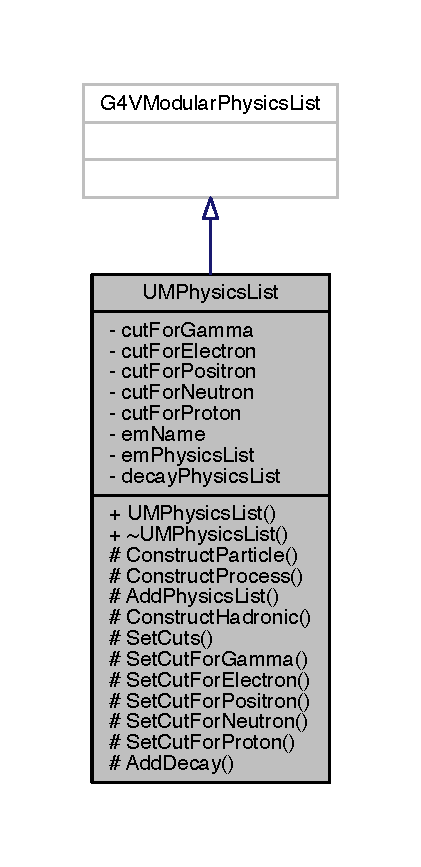
\includegraphics[width=202pt]{classUMPhysicsList__inherit__graph}
\end{center}
\end{figure}


Collaboration diagram for U\+M\+Physics\+List\+:
\nopagebreak
\begin{figure}[H]
\begin{center}
\leavevmode
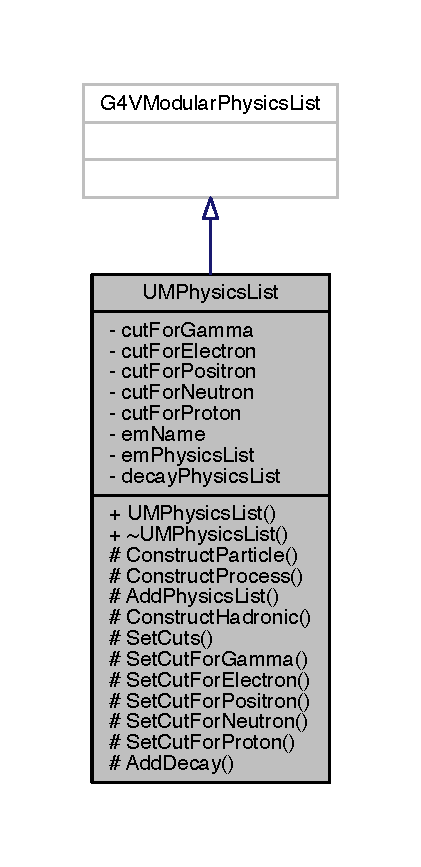
\includegraphics[width=202pt]{classUMPhysicsList__coll__graph}
\end{center}
\end{figure}
\subsection*{Public Member Functions}
\begin{DoxyCompactItemize}
\item 
\hyperlink{classUMPhysicsList_a4284f35908bcd0e3553d7c1395e4cc53}{U\+M\+Physics\+List} ()
\begin{DoxyCompactList}\small\item\em Constructor. \end{DoxyCompactList}\item 
\hyperlink{classUMPhysicsList_af84424dc90d68fe791585d18363f6df6}{$\sim$\+U\+M\+Physics\+List} ()
\begin{DoxyCompactList}\small\item\em Destructor. \end{DoxyCompactList}\end{DoxyCompactItemize}
\subsection*{Protected Member Functions}
\begin{DoxyCompactItemize}
\item 
void \hyperlink{classUMPhysicsList_a3d9f5a9dae553a1d474e8f22860a1ba3}{Construct\+Particle} ()
\begin{DoxyCompactList}\small\item\em Construct particle and physics (mandatory) \end{DoxyCompactList}\item 
void \hyperlink{classUMPhysicsList_a12757c54b86f49f82f9361467f0dcab1}{Construct\+Process} ()
\item 
void \hyperlink{classUMPhysicsList_a4fa74e9c6ebb36baeb975eff3d46af78}{Add\+Physics\+List} (const G4\+String \&name)
\item 
void \hyperlink{classUMPhysicsList_afb0c2f5e798769d9311d94ef25ac4196}{Construct\+Hadronic} ()
\item 
void \hyperlink{classUMPhysicsList_a53bfbb22fa66112d17dd5145a6567b95}{Set\+Cuts} ()
\item 
void \hyperlink{classUMPhysicsList_ab0b676bdb215ef0f4d33870692e9c932}{Set\+Cut\+For\+Gamma} (G4double)
\item 
void \hyperlink{classUMPhysicsList_aa910cc54caf73cb121ba3101079404df}{Set\+Cut\+For\+Electron} (G4double)
\item 
void \hyperlink{classUMPhysicsList_a241f9a0966e58591c2670b84127effa9}{Set\+Cut\+For\+Positron} (G4double)
\item 
void \hyperlink{classUMPhysicsList_abd53a8065177046859b5667e52fe88a9}{Set\+Cut\+For\+Neutron} (G4double)
\item 
void \hyperlink{classUMPhysicsList_ac44692e5e078e015f1bef67525791a5b}{Set\+Cut\+For\+Proton} (G4double)
\item 
void \hyperlink{classUMPhysicsList_ab66c1fa0a2b203bda573e40c63ca46ae}{Add\+Decay} ()
\end{DoxyCompactItemize}
\subsection*{Private Attributes}
\begin{DoxyCompactItemize}
\item 
G4double \hyperlink{classUMPhysicsList_abdb6c5c21e072365e2fac99a3dfed79a}{cut\+For\+Gamma}
\item 
G4double \hyperlink{classUMPhysicsList_a5f93dd2eac07185be039f69e323f7358}{cut\+For\+Electron}
\item 
G4double \hyperlink{classUMPhysicsList_af4ddc9213a3975bfb551034aeb064a87}{cut\+For\+Positron}
\item 
G4double \hyperlink{classUMPhysicsList_a1abce92c27a7f9f647fc986b26af2514}{cut\+For\+Neutron}
\item 
G4double \hyperlink{classUMPhysicsList_aca6ff193291c0c1ff20bdcc292d9dfb1}{cut\+For\+Proton}
\item 
G4\+String \hyperlink{classUMPhysicsList_a59f1eac1b72e641fff39c5d51590f3dc}{em\+Name}
\item 
G4\+V\+Physics\+Constructor $\ast$ \hyperlink{classUMPhysicsList_ac94accb41c3f5cd8eb34019dfdabfbed}{em\+Physics\+List}
\item 
G4\+V\+Physics\+Constructor $\ast$ \hyperlink{classUMPhysicsList_a2c49954b54f069232abe313289d47c87}{decay\+Physics\+List}
\end{DoxyCompactItemize}


\subsection{Detailed Description}
\hyperlink{classUMPhysicsList}{U\+M\+Physics\+List} inherits from G4\+V\+Modular\+Physics\+List 

\subsection{Constructor \& Destructor Documentation}
\hypertarget{classUMPhysicsList_a4284f35908bcd0e3553d7c1395e4cc53}{}\index{U\+M\+Physics\+List@{U\+M\+Physics\+List}!U\+M\+Physics\+List@{U\+M\+Physics\+List}}
\index{U\+M\+Physics\+List@{U\+M\+Physics\+List}!U\+M\+Physics\+List@{U\+M\+Physics\+List}}
\subsubsection[{U\+M\+Physics\+List()}]{\setlength{\rightskip}{0pt plus 5cm}U\+M\+Physics\+List\+::\+U\+M\+Physics\+List (
\begin{DoxyParamCaption}
{}
\end{DoxyParamCaption}
)}\label{classUMPhysicsList_a4284f35908bcd0e3553d7c1395e4cc53}


Constructor. 

Source file for \begin{DoxySeeAlso}{See also}
\hyperlink{classUMPhysicsList}{U\+M\+Physics\+List} This is used for photons!
\end{DoxySeeAlso}
\begin{DoxyAuthor}{Author}
Nikolaos Karastathis $<$ nkarast .at. cern .dot. ch $>$ 
\end{DoxyAuthor}
\begin{DoxyVersion}{Version}
v2.\+0 
\end{DoxyVersion}
E\+M physics \+: Em\+Penelope + Decay\+Physics \hypertarget{classUMPhysicsList_af84424dc90d68fe791585d18363f6df6}{}\index{U\+M\+Physics\+List@{U\+M\+Physics\+List}!````~U\+M\+Physics\+List@{$\sim$\+U\+M\+Physics\+List}}
\index{````~U\+M\+Physics\+List@{$\sim$\+U\+M\+Physics\+List}!U\+M\+Physics\+List@{U\+M\+Physics\+List}}
\subsubsection[{$\sim$\+U\+M\+Physics\+List()}]{\setlength{\rightskip}{0pt plus 5cm}U\+M\+Physics\+List\+::$\sim$\+U\+M\+Physics\+List (
\begin{DoxyParamCaption}
{}
\end{DoxyParamCaption}
)}\label{classUMPhysicsList_af84424dc90d68fe791585d18363f6df6}


Destructor. 



\subsection{Member Function Documentation}
\hypertarget{classUMPhysicsList_ab66c1fa0a2b203bda573e40c63ca46ae}{}\index{U\+M\+Physics\+List@{U\+M\+Physics\+List}!Add\+Decay@{Add\+Decay}}
\index{Add\+Decay@{Add\+Decay}!U\+M\+Physics\+List@{U\+M\+Physics\+List}}
\subsubsection[{Add\+Decay()}]{\setlength{\rightskip}{0pt plus 5cm}void U\+M\+Physics\+List\+::\+Add\+Decay (
\begin{DoxyParamCaption}
{}
\end{DoxyParamCaption}
)\hspace{0.3cm}{\ttfamily [protected]}}\label{classUMPhysicsList_ab66c1fa0a2b203bda573e40c63ca46ae}
decay process

set ordering for Post\+Step\+Do\+It and At\+Rest\+Do\+It \hypertarget{classUMPhysicsList_a4fa74e9c6ebb36baeb975eff3d46af78}{}\index{U\+M\+Physics\+List@{U\+M\+Physics\+List}!Add\+Physics\+List@{Add\+Physics\+List}}
\index{Add\+Physics\+List@{Add\+Physics\+List}!U\+M\+Physics\+List@{U\+M\+Physics\+List}}
\subsubsection[{Add\+Physics\+List(const G4\+String \&name)}]{\setlength{\rightskip}{0pt plus 5cm}void U\+M\+Physics\+List\+::\+Add\+Physics\+List (
\begin{DoxyParamCaption}
\item[{const G4\+String \&}]{name}
\end{DoxyParamCaption}
)\hspace{0.3cm}{\ttfamily [protected]}}\label{classUMPhysicsList_a4fa74e9c6ebb36baeb975eff3d46af78}
\hypertarget{classUMPhysicsList_afb0c2f5e798769d9311d94ef25ac4196}{}\index{U\+M\+Physics\+List@{U\+M\+Physics\+List}!Construct\+Hadronic@{Construct\+Hadronic}}
\index{Construct\+Hadronic@{Construct\+Hadronic}!U\+M\+Physics\+List@{U\+M\+Physics\+List}}
\subsubsection[{Construct\+Hadronic()}]{\setlength{\rightskip}{0pt plus 5cm}void U\+M\+Physics\+List\+::\+Construct\+Hadronic (
\begin{DoxyParamCaption}
{}
\end{DoxyParamCaption}
)\hspace{0.3cm}{\ttfamily [protected]}}\label{classUMPhysicsList_afb0c2f5e798769d9311d94ef25ac4196}
\hypertarget{classUMPhysicsList_a3d9f5a9dae553a1d474e8f22860a1ba3}{}\index{U\+M\+Physics\+List@{U\+M\+Physics\+List}!Construct\+Particle@{Construct\+Particle}}
\index{Construct\+Particle@{Construct\+Particle}!U\+M\+Physics\+List@{U\+M\+Physics\+List}}
\subsubsection[{Construct\+Particle()}]{\setlength{\rightskip}{0pt plus 5cm}void U\+M\+Physics\+List\+::\+Construct\+Particle (
\begin{DoxyParamCaption}
{}
\end{DoxyParamCaption}
)\hspace{0.3cm}{\ttfamily [protected]}}\label{classUMPhysicsList_a3d9f5a9dae553a1d474e8f22860a1ba3}


Construct particle and physics (mandatory) 

\{In this method, static member functions should be called for all particles which you want to use. This ensures that objects of these particle types will be created in the program. \} \hypertarget{classUMPhysicsList_a12757c54b86f49f82f9361467f0dcab1}{}\index{U\+M\+Physics\+List@{U\+M\+Physics\+List}!Construct\+Process@{Construct\+Process}}
\index{Construct\+Process@{Construct\+Process}!U\+M\+Physics\+List@{U\+M\+Physics\+List}}
\subsubsection[{Construct\+Process()}]{\setlength{\rightskip}{0pt plus 5cm}void U\+M\+Physics\+List\+::\+Construct\+Process (
\begin{DoxyParamCaption}
{}
\end{DoxyParamCaption}
)\hspace{0.3cm}{\ttfamily [protected]}}\label{classUMPhysicsList_a12757c54b86f49f82f9361467f0dcab1}
electromagnetic physics list\hypertarget{classUMPhysicsList_aa910cc54caf73cb121ba3101079404df}{}\index{U\+M\+Physics\+List@{U\+M\+Physics\+List}!Set\+Cut\+For\+Electron@{Set\+Cut\+For\+Electron}}
\index{Set\+Cut\+For\+Electron@{Set\+Cut\+For\+Electron}!U\+M\+Physics\+List@{U\+M\+Physics\+List}}
\subsubsection[{Set\+Cut\+For\+Electron(\+G4double)}]{\setlength{\rightskip}{0pt plus 5cm}void U\+M\+Physics\+List\+::\+Set\+Cut\+For\+Electron (
\begin{DoxyParamCaption}
\item[{G4double}]{}
\end{DoxyParamCaption}
)\hspace{0.3cm}{\ttfamily [protected]}}\label{classUMPhysicsList_aa910cc54caf73cb121ba3101079404df}
\hypertarget{classUMPhysicsList_ab0b676bdb215ef0f4d33870692e9c932}{}\index{U\+M\+Physics\+List@{U\+M\+Physics\+List}!Set\+Cut\+For\+Gamma@{Set\+Cut\+For\+Gamma}}
\index{Set\+Cut\+For\+Gamma@{Set\+Cut\+For\+Gamma}!U\+M\+Physics\+List@{U\+M\+Physics\+List}}
\subsubsection[{Set\+Cut\+For\+Gamma(\+G4double)}]{\setlength{\rightskip}{0pt plus 5cm}void U\+M\+Physics\+List\+::\+Set\+Cut\+For\+Gamma (
\begin{DoxyParamCaption}
\item[{G4double}]{}
\end{DoxyParamCaption}
)\hspace{0.3cm}{\ttfamily [protected]}}\label{classUMPhysicsList_ab0b676bdb215ef0f4d33870692e9c932}
\hypertarget{classUMPhysicsList_abd53a8065177046859b5667e52fe88a9}{}\index{U\+M\+Physics\+List@{U\+M\+Physics\+List}!Set\+Cut\+For\+Neutron@{Set\+Cut\+For\+Neutron}}
\index{Set\+Cut\+For\+Neutron@{Set\+Cut\+For\+Neutron}!U\+M\+Physics\+List@{U\+M\+Physics\+List}}
\subsubsection[{Set\+Cut\+For\+Neutron(\+G4double)}]{\setlength{\rightskip}{0pt plus 5cm}void U\+M\+Physics\+List\+::\+Set\+Cut\+For\+Neutron (
\begin{DoxyParamCaption}
\item[{G4double}]{}
\end{DoxyParamCaption}
)\hspace{0.3cm}{\ttfamily [protected]}}\label{classUMPhysicsList_abd53a8065177046859b5667e52fe88a9}
\hypertarget{classUMPhysicsList_a241f9a0966e58591c2670b84127effa9}{}\index{U\+M\+Physics\+List@{U\+M\+Physics\+List}!Set\+Cut\+For\+Positron@{Set\+Cut\+For\+Positron}}
\index{Set\+Cut\+For\+Positron@{Set\+Cut\+For\+Positron}!U\+M\+Physics\+List@{U\+M\+Physics\+List}}
\subsubsection[{Set\+Cut\+For\+Positron(\+G4double)}]{\setlength{\rightskip}{0pt plus 5cm}void U\+M\+Physics\+List\+::\+Set\+Cut\+For\+Positron (
\begin{DoxyParamCaption}
\item[{G4double}]{}
\end{DoxyParamCaption}
)\hspace{0.3cm}{\ttfamily [protected]}}\label{classUMPhysicsList_a241f9a0966e58591c2670b84127effa9}
\hypertarget{classUMPhysicsList_ac44692e5e078e015f1bef67525791a5b}{}\index{U\+M\+Physics\+List@{U\+M\+Physics\+List}!Set\+Cut\+For\+Proton@{Set\+Cut\+For\+Proton}}
\index{Set\+Cut\+For\+Proton@{Set\+Cut\+For\+Proton}!U\+M\+Physics\+List@{U\+M\+Physics\+List}}
\subsubsection[{Set\+Cut\+For\+Proton(\+G4double)}]{\setlength{\rightskip}{0pt plus 5cm}void U\+M\+Physics\+List\+::\+Set\+Cut\+For\+Proton (
\begin{DoxyParamCaption}
\item[{G4double}]{}
\end{DoxyParamCaption}
)\hspace{0.3cm}{\ttfamily [protected]}}\label{classUMPhysicsList_ac44692e5e078e015f1bef67525791a5b}
\hypertarget{classUMPhysicsList_a53bfbb22fa66112d17dd5145a6567b95}{}\index{U\+M\+Physics\+List@{U\+M\+Physics\+List}!Set\+Cuts@{Set\+Cuts}}
\index{Set\+Cuts@{Set\+Cuts}!U\+M\+Physics\+List@{U\+M\+Physics\+List}}
\subsubsection[{Set\+Cuts()}]{\setlength{\rightskip}{0pt plus 5cm}void U\+M\+Physics\+List\+::\+Set\+Cuts (
\begin{DoxyParamCaption}
{}
\end{DoxyParamCaption}
)\hspace{0.3cm}{\ttfamily [protected]}}\label{classUMPhysicsList_a53bfbb22fa66112d17dd5145a6567b95}
pass 

\subsection{Field Documentation}
\hypertarget{classUMPhysicsList_a5f93dd2eac07185be039f69e323f7358}{}\index{U\+M\+Physics\+List@{U\+M\+Physics\+List}!cut\+For\+Electron@{cut\+For\+Electron}}
\index{cut\+For\+Electron@{cut\+For\+Electron}!U\+M\+Physics\+List@{U\+M\+Physics\+List}}
\subsubsection[{cut\+For\+Electron}]{\setlength{\rightskip}{0pt plus 5cm}G4double U\+M\+Physics\+List\+::cut\+For\+Electron\hspace{0.3cm}{\ttfamily [private]}}\label{classUMPhysicsList_a5f93dd2eac07185be039f69e323f7358}
\hypertarget{classUMPhysicsList_abdb6c5c21e072365e2fac99a3dfed79a}{}\index{U\+M\+Physics\+List@{U\+M\+Physics\+List}!cut\+For\+Gamma@{cut\+For\+Gamma}}
\index{cut\+For\+Gamma@{cut\+For\+Gamma}!U\+M\+Physics\+List@{U\+M\+Physics\+List}}
\subsubsection[{cut\+For\+Gamma}]{\setlength{\rightskip}{0pt plus 5cm}G4double U\+M\+Physics\+List\+::cut\+For\+Gamma\hspace{0.3cm}{\ttfamily [private]}}\label{classUMPhysicsList_abdb6c5c21e072365e2fac99a3dfed79a}
\hypertarget{classUMPhysicsList_a1abce92c27a7f9f647fc986b26af2514}{}\index{U\+M\+Physics\+List@{U\+M\+Physics\+List}!cut\+For\+Neutron@{cut\+For\+Neutron}}
\index{cut\+For\+Neutron@{cut\+For\+Neutron}!U\+M\+Physics\+List@{U\+M\+Physics\+List}}
\subsubsection[{cut\+For\+Neutron}]{\setlength{\rightskip}{0pt plus 5cm}G4double U\+M\+Physics\+List\+::cut\+For\+Neutron\hspace{0.3cm}{\ttfamily [private]}}\label{classUMPhysicsList_a1abce92c27a7f9f647fc986b26af2514}
\hypertarget{classUMPhysicsList_af4ddc9213a3975bfb551034aeb064a87}{}\index{U\+M\+Physics\+List@{U\+M\+Physics\+List}!cut\+For\+Positron@{cut\+For\+Positron}}
\index{cut\+For\+Positron@{cut\+For\+Positron}!U\+M\+Physics\+List@{U\+M\+Physics\+List}}
\subsubsection[{cut\+For\+Positron}]{\setlength{\rightskip}{0pt plus 5cm}G4double U\+M\+Physics\+List\+::cut\+For\+Positron\hspace{0.3cm}{\ttfamily [private]}}\label{classUMPhysicsList_af4ddc9213a3975bfb551034aeb064a87}
\hypertarget{classUMPhysicsList_aca6ff193291c0c1ff20bdcc292d9dfb1}{}\index{U\+M\+Physics\+List@{U\+M\+Physics\+List}!cut\+For\+Proton@{cut\+For\+Proton}}
\index{cut\+For\+Proton@{cut\+For\+Proton}!U\+M\+Physics\+List@{U\+M\+Physics\+List}}
\subsubsection[{cut\+For\+Proton}]{\setlength{\rightskip}{0pt plus 5cm}G4double U\+M\+Physics\+List\+::cut\+For\+Proton\hspace{0.3cm}{\ttfamily [private]}}\label{classUMPhysicsList_aca6ff193291c0c1ff20bdcc292d9dfb1}
\hypertarget{classUMPhysicsList_a2c49954b54f069232abe313289d47c87}{}\index{U\+M\+Physics\+List@{U\+M\+Physics\+List}!decay\+Physics\+List@{decay\+Physics\+List}}
\index{decay\+Physics\+List@{decay\+Physics\+List}!U\+M\+Physics\+List@{U\+M\+Physics\+List}}
\subsubsection[{decay\+Physics\+List}]{\setlength{\rightskip}{0pt plus 5cm}G4\+V\+Physics\+Constructor$\ast$ U\+M\+Physics\+List\+::decay\+Physics\+List\hspace{0.3cm}{\ttfamily [private]}}\label{classUMPhysicsList_a2c49954b54f069232abe313289d47c87}
\hypertarget{classUMPhysicsList_a59f1eac1b72e641fff39c5d51590f3dc}{}\index{U\+M\+Physics\+List@{U\+M\+Physics\+List}!em\+Name@{em\+Name}}
\index{em\+Name@{em\+Name}!U\+M\+Physics\+List@{U\+M\+Physics\+List}}
\subsubsection[{em\+Name}]{\setlength{\rightskip}{0pt plus 5cm}G4\+String U\+M\+Physics\+List\+::em\+Name\hspace{0.3cm}{\ttfamily [private]}}\label{classUMPhysicsList_a59f1eac1b72e641fff39c5d51590f3dc}
\hypertarget{classUMPhysicsList_ac94accb41c3f5cd8eb34019dfdabfbed}{}\index{U\+M\+Physics\+List@{U\+M\+Physics\+List}!em\+Physics\+List@{em\+Physics\+List}}
\index{em\+Physics\+List@{em\+Physics\+List}!U\+M\+Physics\+List@{U\+M\+Physics\+List}}
\subsubsection[{em\+Physics\+List}]{\setlength{\rightskip}{0pt plus 5cm}G4\+V\+Physics\+Constructor$\ast$ U\+M\+Physics\+List\+::em\+Physics\+List\hspace{0.3cm}{\ttfamily [private]}}\label{classUMPhysicsList_ac94accb41c3f5cd8eb34019dfdabfbed}


The documentation for this class was generated from the following files\+:\begin{DoxyCompactItemize}
\item 
include/\hyperlink{UMPhysicsList_8hh}{U\+M\+Physics\+List.\+hh}\item 
src/\hyperlink{UMPhysicsList_8cc}{U\+M\+Physics\+List.\+cc}\end{DoxyCompactItemize}

\hypertarget{classUMPrimaryGeneratorAction}{}\section{U\+M\+Primary\+Generator\+Action Class Reference}
\label{classUMPrimaryGeneratorAction}\index{U\+M\+Primary\+Generator\+Action@{U\+M\+Primary\+Generator\+Action}}


{\ttfamily \#include $<$U\+M\+Primary\+Generator\+Action.\+hh$>$}



Inheritance diagram for U\+M\+Primary\+Generator\+Action\+:
\nopagebreak
\begin{figure}[H]
\begin{center}
\leavevmode
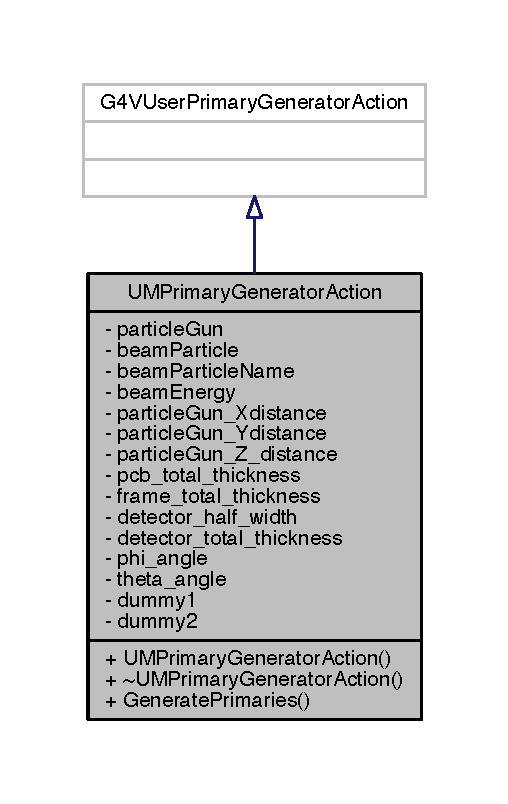
\includegraphics[width=244pt]{classUMPrimaryGeneratorAction__inherit__graph}
\end{center}
\end{figure}


Collaboration diagram for U\+M\+Primary\+Generator\+Action\+:
\nopagebreak
\begin{figure}[H]
\begin{center}
\leavevmode
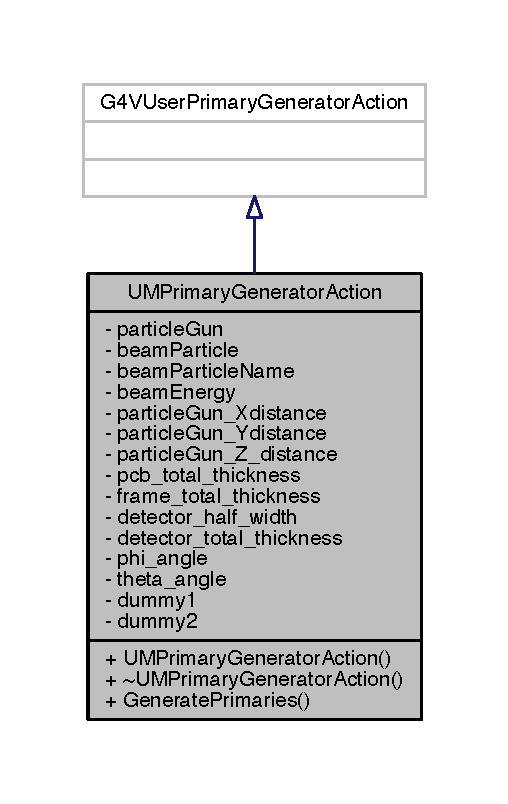
\includegraphics[width=244pt]{classUMPrimaryGeneratorAction__coll__graph}
\end{center}
\end{figure}
\subsection*{Public Member Functions}
\begin{DoxyCompactItemize}
\item 
\hyperlink{classUMPrimaryGeneratorAction_a2be9dfff9f8b8142a3c550503647cd4e}{U\+M\+Primary\+Generator\+Action} ()
\item 
virtual \hyperlink{classUMPrimaryGeneratorAction_a2da0583ffcf7339c335beeadf33b0bcb}{$\sim$\+U\+M\+Primary\+Generator\+Action} ()
\item 
void \hyperlink{classUMPrimaryGeneratorAction_a40f908530ea769019180454cfe529d22}{Generate\+Primaries} (G4\+Event $\ast$an\+Event)
\end{DoxyCompactItemize}
\subsection*{Private Attributes}
\begin{DoxyCompactItemize}
\item 
G4\+Particle\+Gun $\ast$ \hyperlink{classUMPrimaryGeneratorAction_a787ca62e699ace1aa9cae6c42c9d7743}{particle\+Gun}
\item 
G4\+Particle\+Definition $\ast$ \hyperlink{classUMPrimaryGeneratorAction_a004f6a76d578f065cee7a3f1e1228abd}{beam\+Particle}
\begin{DoxyCompactList}\small\item\em some definitions \end{DoxyCompactList}\item 
G4\+String \hyperlink{classUMPrimaryGeneratorAction_aec782ea37985870020b9428534785a9b}{beam\+Particle\+Name}
\item 
G4double \hyperlink{classUMPrimaryGeneratorAction_a59b85366f8c349e736250e532d231e67}{beam\+Energy}
\item 
G4double \hyperlink{classUMPrimaryGeneratorAction_a10ad8439cfae25861c154f7c983d69c7}{particle\+Gun\+\_\+\+Xdistance}
\item 
G4double \hyperlink{classUMPrimaryGeneratorAction_ad8ca25605dc9d53d6f4c458bc53c9286}{particle\+Gun\+\_\+\+Ydistance}
\item 
G4double \hyperlink{classUMPrimaryGeneratorAction_a655f1759775835e3e687e8a9fdfd1889}{particle\+Gun\+\_\+\+Z\+\_\+distance}
\item 
G4double \hyperlink{classUMPrimaryGeneratorAction_a82995abaa2c42648522cacf20f9a9f4f}{pcb\+\_\+total\+\_\+thickness}
\item 
G4double \hyperlink{classUMPrimaryGeneratorAction_a9cfba814762d43a22df9b2da505d23c3}{frame\+\_\+total\+\_\+thickness}
\item 
G4double \hyperlink{classUMPrimaryGeneratorAction_a25173fd11d4081d650b3943cd52fe933}{detector\+\_\+half\+\_\+width}
\item 
G4double \hyperlink{classUMPrimaryGeneratorAction_acf85442c095148faf0055372cc70911d}{detector\+\_\+total\+\_\+thickness}
\item 
G4double \hyperlink{classUMPrimaryGeneratorAction_a4de1dd00da08850d4d260248fff6f2ae}{phi\+\_\+angle}
\item 
G4double \hyperlink{classUMPrimaryGeneratorAction_a254fcb36e5b52349847120db69071ec9}{theta\+\_\+angle}
\item 
G4double \hyperlink{classUMPrimaryGeneratorAction_a8fdaaf24898f8c34087558bc4c740b55}{dummy1}
\item 
G4double \hyperlink{classUMPrimaryGeneratorAction_ade806eed80671f071afebf82e0a8ad68}{dummy2}
\end{DoxyCompactItemize}


\subsection{Constructor \& Destructor Documentation}
\hypertarget{classUMPrimaryGeneratorAction_a2be9dfff9f8b8142a3c550503647cd4e}{}\index{U\+M\+Primary\+Generator\+Action@{U\+M\+Primary\+Generator\+Action}!U\+M\+Primary\+Generator\+Action@{U\+M\+Primary\+Generator\+Action}}
\index{U\+M\+Primary\+Generator\+Action@{U\+M\+Primary\+Generator\+Action}!U\+M\+Primary\+Generator\+Action@{U\+M\+Primary\+Generator\+Action}}
\subsubsection[{U\+M\+Primary\+Generator\+Action()}]{\setlength{\rightskip}{0pt plus 5cm}U\+M\+Primary\+Generator\+Action\+::\+U\+M\+Primary\+Generator\+Action (
\begin{DoxyParamCaption}
{}
\end{DoxyParamCaption}
)}\label{classUMPrimaryGeneratorAction_a2be9dfff9f8b8142a3c550503647cd4e}
Source file for \begin{DoxySeeAlso}{See also}
\hyperlink{classUMPrimaryGeneratorAction}{U\+M\+Primary\+Generator\+Action}
\end{DoxySeeAlso}
\begin{DoxyAuthor}{Author}
Nikolaos Karastathis $<$ nkarast .at. cern .dot. ch $>$ 
\end{DoxyAuthor}
\begin{DoxyVersion}{Version}
v2.\+0 
\end{DoxyVersion}
\hypertarget{classUMPrimaryGeneratorAction_a2da0583ffcf7339c335beeadf33b0bcb}{}\index{U\+M\+Primary\+Generator\+Action@{U\+M\+Primary\+Generator\+Action}!````~U\+M\+Primary\+Generator\+Action@{$\sim$\+U\+M\+Primary\+Generator\+Action}}
\index{````~U\+M\+Primary\+Generator\+Action@{$\sim$\+U\+M\+Primary\+Generator\+Action}!U\+M\+Primary\+Generator\+Action@{U\+M\+Primary\+Generator\+Action}}
\subsubsection[{$\sim$\+U\+M\+Primary\+Generator\+Action()}]{\setlength{\rightskip}{0pt plus 5cm}U\+M\+Primary\+Generator\+Action\+::$\sim$\+U\+M\+Primary\+Generator\+Action (
\begin{DoxyParamCaption}
{}
\end{DoxyParamCaption}
)\hspace{0.3cm}{\ttfamily [virtual]}}\label{classUMPrimaryGeneratorAction_a2da0583ffcf7339c335beeadf33b0bcb}


\subsection{Member Function Documentation}
\hypertarget{classUMPrimaryGeneratorAction_a40f908530ea769019180454cfe529d22}{}\index{U\+M\+Primary\+Generator\+Action@{U\+M\+Primary\+Generator\+Action}!Generate\+Primaries@{Generate\+Primaries}}
\index{Generate\+Primaries@{Generate\+Primaries}!U\+M\+Primary\+Generator\+Action@{U\+M\+Primary\+Generator\+Action}}
\subsubsection[{Generate\+Primaries(\+G4\+Event $\ast$an\+Event)}]{\setlength{\rightskip}{0pt plus 5cm}void U\+M\+Primary\+Generator\+Action\+::\+Generate\+Primaries (
\begin{DoxyParamCaption}
\item[{G4\+Event $\ast$}]{an\+Event}
\end{DoxyParamCaption}
)}\label{classUMPrimaryGeneratorAction_a40f908530ea769019180454cfe529d22}
\begin{DoxyAttention}{Attention}
\{C\+A\+R\+E\+F\+U\+L\+L A\+B\+O\+U\+T T\+H\+E Y P\+O\+S\+I\+T\+I\+O\+N H\+E\+R\+E! -- This is set for A\+N\+G\+U\+L\+A\+R B\+E\+A\+M\+S!\}
\end{DoxyAttention}
the particle gun is particle\+Gun\+\_\+\+Xdistance away from the C\+E\+N\+T\+E\+R of the detector but the maximum opening distance would be aquired if we calculate the angles with respect to the first frame that the particle impacts ===$>$$>$ to calculate the angles we subtract the half\+\_\+width of the detector

set the momentum of X-\/axis towards the negative direction

now that everything is setup generate an event! 

\subsection{Field Documentation}
\hypertarget{classUMPrimaryGeneratorAction_a59b85366f8c349e736250e532d231e67}{}\index{U\+M\+Primary\+Generator\+Action@{U\+M\+Primary\+Generator\+Action}!beam\+Energy@{beam\+Energy}}
\index{beam\+Energy@{beam\+Energy}!U\+M\+Primary\+Generator\+Action@{U\+M\+Primary\+Generator\+Action}}
\subsubsection[{beam\+Energy}]{\setlength{\rightskip}{0pt plus 5cm}G4double U\+M\+Primary\+Generator\+Action\+::beam\+Energy\hspace{0.3cm}{\ttfamily [private]}}\label{classUMPrimaryGeneratorAction_a59b85366f8c349e736250e532d231e67}
\hypertarget{classUMPrimaryGeneratorAction_a004f6a76d578f065cee7a3f1e1228abd}{}\index{U\+M\+Primary\+Generator\+Action@{U\+M\+Primary\+Generator\+Action}!beam\+Particle@{beam\+Particle}}
\index{beam\+Particle@{beam\+Particle}!U\+M\+Primary\+Generator\+Action@{U\+M\+Primary\+Generator\+Action}}
\subsubsection[{beam\+Particle}]{\setlength{\rightskip}{0pt plus 5cm}G4\+Particle\+Definition$\ast$ U\+M\+Primary\+Generator\+Action\+::beam\+Particle\hspace{0.3cm}{\ttfamily [private]}}\label{classUMPrimaryGeneratorAction_a004f6a76d578f065cee7a3f1e1228abd}


some definitions 

\hypertarget{classUMPrimaryGeneratorAction_aec782ea37985870020b9428534785a9b}{}\index{U\+M\+Primary\+Generator\+Action@{U\+M\+Primary\+Generator\+Action}!beam\+Particle\+Name@{beam\+Particle\+Name}}
\index{beam\+Particle\+Name@{beam\+Particle\+Name}!U\+M\+Primary\+Generator\+Action@{U\+M\+Primary\+Generator\+Action}}
\subsubsection[{beam\+Particle\+Name}]{\setlength{\rightskip}{0pt plus 5cm}G4\+String U\+M\+Primary\+Generator\+Action\+::beam\+Particle\+Name\hspace{0.3cm}{\ttfamily [private]}}\label{classUMPrimaryGeneratorAction_aec782ea37985870020b9428534785a9b}
\hypertarget{classUMPrimaryGeneratorAction_a25173fd11d4081d650b3943cd52fe933}{}\index{U\+M\+Primary\+Generator\+Action@{U\+M\+Primary\+Generator\+Action}!detector\+\_\+half\+\_\+width@{detector\+\_\+half\+\_\+width}}
\index{detector\+\_\+half\+\_\+width@{detector\+\_\+half\+\_\+width}!U\+M\+Primary\+Generator\+Action@{U\+M\+Primary\+Generator\+Action}}
\subsubsection[{detector\+\_\+half\+\_\+width}]{\setlength{\rightskip}{0pt plus 5cm}G4double U\+M\+Primary\+Generator\+Action\+::detector\+\_\+half\+\_\+width\hspace{0.3cm}{\ttfamily [private]}}\label{classUMPrimaryGeneratorAction_a25173fd11d4081d650b3943cd52fe933}
\hypertarget{classUMPrimaryGeneratorAction_acf85442c095148faf0055372cc70911d}{}\index{U\+M\+Primary\+Generator\+Action@{U\+M\+Primary\+Generator\+Action}!detector\+\_\+total\+\_\+thickness@{detector\+\_\+total\+\_\+thickness}}
\index{detector\+\_\+total\+\_\+thickness@{detector\+\_\+total\+\_\+thickness}!U\+M\+Primary\+Generator\+Action@{U\+M\+Primary\+Generator\+Action}}
\subsubsection[{detector\+\_\+total\+\_\+thickness}]{\setlength{\rightskip}{0pt plus 5cm}G4double U\+M\+Primary\+Generator\+Action\+::detector\+\_\+total\+\_\+thickness\hspace{0.3cm}{\ttfamily [private]}}\label{classUMPrimaryGeneratorAction_acf85442c095148faf0055372cc70911d}
\hypertarget{classUMPrimaryGeneratorAction_a8fdaaf24898f8c34087558bc4c740b55}{}\index{U\+M\+Primary\+Generator\+Action@{U\+M\+Primary\+Generator\+Action}!dummy1@{dummy1}}
\index{dummy1@{dummy1}!U\+M\+Primary\+Generator\+Action@{U\+M\+Primary\+Generator\+Action}}
\subsubsection[{dummy1}]{\setlength{\rightskip}{0pt plus 5cm}G4double U\+M\+Primary\+Generator\+Action\+::dummy1\hspace{0.3cm}{\ttfamily [private]}}\label{classUMPrimaryGeneratorAction_a8fdaaf24898f8c34087558bc4c740b55}
\hypertarget{classUMPrimaryGeneratorAction_ade806eed80671f071afebf82e0a8ad68}{}\index{U\+M\+Primary\+Generator\+Action@{U\+M\+Primary\+Generator\+Action}!dummy2@{dummy2}}
\index{dummy2@{dummy2}!U\+M\+Primary\+Generator\+Action@{U\+M\+Primary\+Generator\+Action}}
\subsubsection[{dummy2}]{\setlength{\rightskip}{0pt plus 5cm}G4double U\+M\+Primary\+Generator\+Action\+::dummy2\hspace{0.3cm}{\ttfamily [private]}}\label{classUMPrimaryGeneratorAction_ade806eed80671f071afebf82e0a8ad68}
\hypertarget{classUMPrimaryGeneratorAction_a9cfba814762d43a22df9b2da505d23c3}{}\index{U\+M\+Primary\+Generator\+Action@{U\+M\+Primary\+Generator\+Action}!frame\+\_\+total\+\_\+thickness@{frame\+\_\+total\+\_\+thickness}}
\index{frame\+\_\+total\+\_\+thickness@{frame\+\_\+total\+\_\+thickness}!U\+M\+Primary\+Generator\+Action@{U\+M\+Primary\+Generator\+Action}}
\subsubsection[{frame\+\_\+total\+\_\+thickness}]{\setlength{\rightskip}{0pt plus 5cm}G4double U\+M\+Primary\+Generator\+Action\+::frame\+\_\+total\+\_\+thickness\hspace{0.3cm}{\ttfamily [private]}}\label{classUMPrimaryGeneratorAction_a9cfba814762d43a22df9b2da505d23c3}
\hypertarget{classUMPrimaryGeneratorAction_a787ca62e699ace1aa9cae6c42c9d7743}{}\index{U\+M\+Primary\+Generator\+Action@{U\+M\+Primary\+Generator\+Action}!particle\+Gun@{particle\+Gun}}
\index{particle\+Gun@{particle\+Gun}!U\+M\+Primary\+Generator\+Action@{U\+M\+Primary\+Generator\+Action}}
\subsubsection[{particle\+Gun}]{\setlength{\rightskip}{0pt plus 5cm}G4\+Particle\+Gun$\ast$ U\+M\+Primary\+Generator\+Action\+::particle\+Gun\hspace{0.3cm}{\ttfamily [private]}}\label{classUMPrimaryGeneratorAction_a787ca62e699ace1aa9cae6c42c9d7743}
\hypertarget{classUMPrimaryGeneratorAction_a10ad8439cfae25861c154f7c983d69c7}{}\index{U\+M\+Primary\+Generator\+Action@{U\+M\+Primary\+Generator\+Action}!particle\+Gun\+\_\+\+Xdistance@{particle\+Gun\+\_\+\+Xdistance}}
\index{particle\+Gun\+\_\+\+Xdistance@{particle\+Gun\+\_\+\+Xdistance}!U\+M\+Primary\+Generator\+Action@{U\+M\+Primary\+Generator\+Action}}
\subsubsection[{particle\+Gun\+\_\+\+Xdistance}]{\setlength{\rightskip}{0pt plus 5cm}G4double U\+M\+Primary\+Generator\+Action\+::particle\+Gun\+\_\+\+Xdistance\hspace{0.3cm}{\ttfamily [private]}}\label{classUMPrimaryGeneratorAction_a10ad8439cfae25861c154f7c983d69c7}
\hypertarget{classUMPrimaryGeneratorAction_ad8ca25605dc9d53d6f4c458bc53c9286}{}\index{U\+M\+Primary\+Generator\+Action@{U\+M\+Primary\+Generator\+Action}!particle\+Gun\+\_\+\+Ydistance@{particle\+Gun\+\_\+\+Ydistance}}
\index{particle\+Gun\+\_\+\+Ydistance@{particle\+Gun\+\_\+\+Ydistance}!U\+M\+Primary\+Generator\+Action@{U\+M\+Primary\+Generator\+Action}}
\subsubsection[{particle\+Gun\+\_\+\+Ydistance}]{\setlength{\rightskip}{0pt plus 5cm}G4double U\+M\+Primary\+Generator\+Action\+::particle\+Gun\+\_\+\+Ydistance\hspace{0.3cm}{\ttfamily [private]}}\label{classUMPrimaryGeneratorAction_ad8ca25605dc9d53d6f4c458bc53c9286}
\hypertarget{classUMPrimaryGeneratorAction_a655f1759775835e3e687e8a9fdfd1889}{}\index{U\+M\+Primary\+Generator\+Action@{U\+M\+Primary\+Generator\+Action}!particle\+Gun\+\_\+\+Z\+\_\+distance@{particle\+Gun\+\_\+\+Z\+\_\+distance}}
\index{particle\+Gun\+\_\+\+Z\+\_\+distance@{particle\+Gun\+\_\+\+Z\+\_\+distance}!U\+M\+Primary\+Generator\+Action@{U\+M\+Primary\+Generator\+Action}}
\subsubsection[{particle\+Gun\+\_\+\+Z\+\_\+distance}]{\setlength{\rightskip}{0pt plus 5cm}G4double U\+M\+Primary\+Generator\+Action\+::particle\+Gun\+\_\+\+Z\+\_\+distance\hspace{0.3cm}{\ttfamily [private]}}\label{classUMPrimaryGeneratorAction_a655f1759775835e3e687e8a9fdfd1889}
\hypertarget{classUMPrimaryGeneratorAction_a82995abaa2c42648522cacf20f9a9f4f}{}\index{U\+M\+Primary\+Generator\+Action@{U\+M\+Primary\+Generator\+Action}!pcb\+\_\+total\+\_\+thickness@{pcb\+\_\+total\+\_\+thickness}}
\index{pcb\+\_\+total\+\_\+thickness@{pcb\+\_\+total\+\_\+thickness}!U\+M\+Primary\+Generator\+Action@{U\+M\+Primary\+Generator\+Action}}
\subsubsection[{pcb\+\_\+total\+\_\+thickness}]{\setlength{\rightskip}{0pt plus 5cm}G4double U\+M\+Primary\+Generator\+Action\+::pcb\+\_\+total\+\_\+thickness\hspace{0.3cm}{\ttfamily [private]}}\label{classUMPrimaryGeneratorAction_a82995abaa2c42648522cacf20f9a9f4f}
\hypertarget{classUMPrimaryGeneratorAction_a4de1dd00da08850d4d260248fff6f2ae}{}\index{U\+M\+Primary\+Generator\+Action@{U\+M\+Primary\+Generator\+Action}!phi\+\_\+angle@{phi\+\_\+angle}}
\index{phi\+\_\+angle@{phi\+\_\+angle}!U\+M\+Primary\+Generator\+Action@{U\+M\+Primary\+Generator\+Action}}
\subsubsection[{phi\+\_\+angle}]{\setlength{\rightskip}{0pt plus 5cm}G4double U\+M\+Primary\+Generator\+Action\+::phi\+\_\+angle\hspace{0.3cm}{\ttfamily [private]}}\label{classUMPrimaryGeneratorAction_a4de1dd00da08850d4d260248fff6f2ae}
\hypertarget{classUMPrimaryGeneratorAction_a254fcb36e5b52349847120db69071ec9}{}\index{U\+M\+Primary\+Generator\+Action@{U\+M\+Primary\+Generator\+Action}!theta\+\_\+angle@{theta\+\_\+angle}}
\index{theta\+\_\+angle@{theta\+\_\+angle}!U\+M\+Primary\+Generator\+Action@{U\+M\+Primary\+Generator\+Action}}
\subsubsection[{theta\+\_\+angle}]{\setlength{\rightskip}{0pt plus 5cm}G4double U\+M\+Primary\+Generator\+Action\+::theta\+\_\+angle\hspace{0.3cm}{\ttfamily [private]}}\label{classUMPrimaryGeneratorAction_a254fcb36e5b52349847120db69071ec9}


The documentation for this class was generated from the following files\+:\begin{DoxyCompactItemize}
\item 
include/\hyperlink{UMPrimaryGeneratorAction_8hh}{U\+M\+Primary\+Generator\+Action.\+hh}\item 
src/\hyperlink{UMPrimaryGeneratorAction_8cc}{U\+M\+Primary\+Generator\+Action.\+cc}\end{DoxyCompactItemize}

\hypertarget{classUMRootSaver}{}\section{U\+M\+Root\+Saver Class Reference}
\label{classUMRootSaver}\index{U\+M\+Root\+Saver@{U\+M\+Root\+Saver}}


{\ttfamily \#include $<$U\+M\+Root\+Saver.\+hh$>$}



Collaboration diagram for U\+M\+Root\+Saver\+:
\nopagebreak
\begin{figure}[H]
\begin{center}
\leavevmode
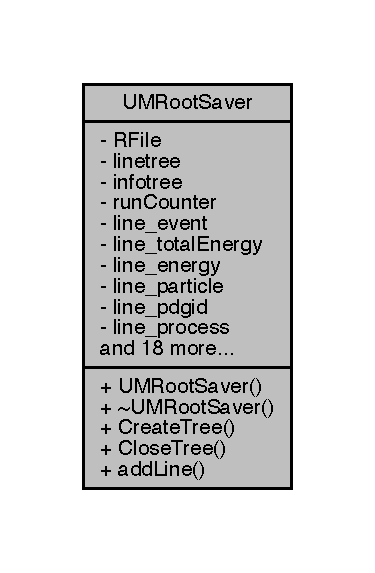
\includegraphics[width=180pt]{classUMRootSaver__coll__graph}
\end{center}
\end{figure}
\subsection*{Public Member Functions}
\begin{DoxyCompactItemize}
\item 
\hyperlink{classUMRootSaver_a96154d44d69b9dc6e0aef05a9f39e7dc}{U\+M\+Root\+Saver} ()
\begin{DoxyCompactList}\small\item\em \{The Class creates a R\+O\+O\+T saver object with two trees to be output\} \end{DoxyCompactList}\item 
virtual \hyperlink{classUMRootSaver_a874c1e2de31c7bde041e5ab6310219ca}{$\sim$\+U\+M\+Root\+Saver} ()
\item 
virtual void \hyperlink{classUMRootSaver_a12b7c7cf3bba7c57b940b7c70566331c}{Create\+Tree} ()
\item 
virtual void \hyperlink{classUMRootSaver_a04707033a436e745215d082ae70c1c3d}{Close\+Tree} ()
\item 
virtual void \hyperlink{classUMRootSaver_a0574c48b931667d328005772a49f2f4e}{add\+Line} (G4int event, G4double energy, G4\+String particle\+Name, G4int pdgid, G4\+String process, G4double xpos, G4double ypos, G4double zpos)
\end{DoxyCompactItemize}
\subsection*{Private Attributes}
\begin{DoxyCompactItemize}
\item 
T\+File $\ast$ \hyperlink{classUMRootSaver_ad7ffe5037296689e41b7c161afa3cee3}{R\+File}
\item 
T\+Tree $\ast$ \hyperlink{classUMRootSaver_a29e193f625e575fdbbb87af833959260}{linetree}
\item 
T\+Tree $\ast$ \hyperlink{classUMRootSaver_a2480f54d6b0013cc940e00b242508747}{infotree}
\item 
unsigned int \hyperlink{classUMRootSaver_a99af4bcf69b6a924398e5f9f4c55dd0f}{run\+Counter}
\item 
int \hyperlink{classUMRootSaver_aa2a036666d57184757bf92a30fa92a01}{line\+\_\+event} = -\/1000
\item 
double \hyperlink{classUMRootSaver_ab4ce203238d77838c94d6e79c8da7627}{line\+\_\+total\+Energy} = 0
\item 
std\+::vector$<$ double $>$ \hyperlink{classUMRootSaver_a3306ae5496af585da4cfcb7b814add17}{line\+\_\+energy}
\item 
std\+::vector$<$ std\+::string $>$ \hyperlink{classUMRootSaver_a238095e0ad1a8ffb1c8234dbd8498267}{line\+\_\+particle}
\item 
std\+::vector$<$ int $>$ \hyperlink{classUMRootSaver_a2a2b886dd46e2c58518a77d17c699ef4}{line\+\_\+pdgid}
\item 
std\+::vector$<$ std\+::string $>$ \hyperlink{classUMRootSaver_a7314b2dbee08811d7c0ffe8da8e6a139}{line\+\_\+process}
\item 
std\+::vector$<$ double $>$ \hyperlink{classUMRootSaver_a2050b402447a170697da61679df4083e}{line\+\_\+xpos}
\item 
std\+::vector$<$ double $>$ \hyperlink{classUMRootSaver_a987f396719a5013af8b6e8ef181ff102}{line\+\_\+ypos}
\item 
std\+::vector$<$ double $>$ \hyperlink{classUMRootSaver_a614b0676af3c14b3539d39dae29ae32e}{line\+\_\+zpos}
\item 
double \hyperlink{classUMRootSaver_add592e7355abbae18ec766a482fcf051}{line\+\_\+above\+\_\+resistive} = 1117.\+0
\item 
double \hyperlink{classUMRootSaver_a3eaefa9c88dfb35ad31f9cbe696deb5d}{line\+\_\+below\+\_\+mesh} = 1216.\+0
\item 
double \hyperlink{classUMRootSaver_ae741b38eda489eefddb6bed3295bf857}{line\+\_\+above\+\_\+mesh} = 1240.\+0
\item 
double \hyperlink{classUMRootSaver_a42a91f0a2e68665dfaa4a084c8b73b4a}{line\+\_\+below\+\_\+drift} = 6216.\+0
\item 
double \hyperlink{classUMRootSaver_a49acbd1dd22d72f9d00c2f262cdc8a2c}{line\+\_\+positivey} = 50000.
\item 
double \hyperlink{classUMRootSaver_a1fa4a2ba095c5dcc794de33f25a42e35}{line\+\_\+negativey} = -\/50000.
\item 
double \hyperlink{classUMRootSaver_a7439f5ed17b1b5d0fac167973db37487}{line\+\_\+positivez} = 50000.
\item 
double \hyperlink{classUMRootSaver_a41e77a03fea64cc18102920f18450979}{line\+\_\+negativez} = -\/50000.
\item 
double \hyperlink{classUMRootSaver_aedc64ce54759ccba3b139b4a1aa3f695}{line\+\_\+positivex} = 23000.
\item 
double \hyperlink{classUMRootSaver_a7792131c2371da76bc184cdd5280213f}{line\+\_\+beam\+\_\+energy} = 0
\item 
double \hyperlink{classUMRootSaver_a4ae1aa5a692e420f7f3180ac34fa2567}{line\+\_\+beam\+\_\+start\+X} = 0
\item 
double \hyperlink{classUMRootSaver_a861a274f7f49bfa59cdbf41f9ea2acc2}{line\+\_\+beam\+\_\+start\+Y} = 0
\item 
double \hyperlink{classUMRootSaver_acd5167ed144e077742582dd8720fb03e}{line\+\_\+beam\+\_\+start\+Z} = 0
\item 
double \hyperlink{classUMRootSaver_a1b94f0a9b4a5ba2c1a640e22e37ec07a}{line\+\_\+\+Argon\+\_\+percent} = 0
\item 
double \hyperlink{classUMRootSaver_a9250e9ecd6587858b397a35bb55a7889}{line\+\_\+\+C\+O2\+\_\+percent} = 0
\end{DoxyCompactItemize}


\subsection{Constructor \& Destructor Documentation}
\hypertarget{classUMRootSaver_a96154d44d69b9dc6e0aef05a9f39e7dc}{}\index{U\+M\+Root\+Saver@{U\+M\+Root\+Saver}!U\+M\+Root\+Saver@{U\+M\+Root\+Saver}}
\index{U\+M\+Root\+Saver@{U\+M\+Root\+Saver}!U\+M\+Root\+Saver@{U\+M\+Root\+Saver}}
\subsubsection[{U\+M\+Root\+Saver()}]{\setlength{\rightskip}{0pt plus 5cm}U\+M\+Root\+Saver\+::\+U\+M\+Root\+Saver (
\begin{DoxyParamCaption}
{}
\end{DoxyParamCaption}
)}\label{classUMRootSaver_a96154d44d69b9dc6e0aef05a9f39e7dc}


\{The Class creates a R\+O\+O\+T saver object with two trees to be output\} 

\hypertarget{classUMRootSaver_a874c1e2de31c7bde041e5ab6310219ca}{}\index{U\+M\+Root\+Saver@{U\+M\+Root\+Saver}!````~U\+M\+Root\+Saver@{$\sim$\+U\+M\+Root\+Saver}}
\index{````~U\+M\+Root\+Saver@{$\sim$\+U\+M\+Root\+Saver}!U\+M\+Root\+Saver@{U\+M\+Root\+Saver}}
\subsubsection[{$\sim$\+U\+M\+Root\+Saver()}]{\setlength{\rightskip}{0pt plus 5cm}U\+M\+Root\+Saver\+::$\sim$\+U\+M\+Root\+Saver (
\begin{DoxyParamCaption}
{}
\end{DoxyParamCaption}
)\hspace{0.3cm}{\ttfamily [virtual]}}\label{classUMRootSaver_a874c1e2de31c7bde041e5ab6310219ca}


\subsection{Member Function Documentation}
\hypertarget{classUMRootSaver_a0574c48b931667d328005772a49f2f4e}{}\index{U\+M\+Root\+Saver@{U\+M\+Root\+Saver}!add\+Line@{add\+Line}}
\index{add\+Line@{add\+Line}!U\+M\+Root\+Saver@{U\+M\+Root\+Saver}}
\subsubsection[{add\+Line(\+G4int event, G4double energy, G4\+String particle\+Name, G4int pdgid, G4\+String process, G4double xpos, G4double ypos, G4double zpos)}]{\setlength{\rightskip}{0pt plus 5cm}void U\+M\+Root\+Saver\+::add\+Line (
\begin{DoxyParamCaption}
\item[{G4int}]{event, }
\item[{G4double}]{energy, }
\item[{G4\+String}]{particle\+Name, }
\item[{G4int}]{pdgid, }
\item[{G4\+String}]{process, }
\item[{G4double}]{xpos, }
\item[{G4double}]{ypos, }
\item[{G4double}]{zpos}
\end{DoxyParamCaption}
)\hspace{0.3cm}{\ttfamily [virtual]}}\label{classUMRootSaver_a0574c48b931667d328005772a49f2f4e}
Imagine that you\textquotesingle{}re writing to a plain txt file... Call this function whenever you want to add a line I\textquotesingle{}ll handle the  ;)

Here is where all the R\+O\+O\+T magic happens \hypertarget{classUMRootSaver_a04707033a436e745215d082ae70c1c3d}{}\index{U\+M\+Root\+Saver@{U\+M\+Root\+Saver}!Close\+Tree@{Close\+Tree}}
\index{Close\+Tree@{Close\+Tree}!U\+M\+Root\+Saver@{U\+M\+Root\+Saver}}
\subsubsection[{Close\+Tree()}]{\setlength{\rightskip}{0pt plus 5cm}void U\+M\+Root\+Saver\+::\+Close\+Tree (
\begin{DoxyParamCaption}
{}
\end{DoxyParamCaption}
)\hspace{0.3cm}{\ttfamily [virtual]}}\label{classUMRootSaver_a04707033a436e745215d082ae70c1c3d}
this is for the last event to be written, since we add one line per {\ttfamily add\+Line} call \hypertarget{classUMRootSaver_a12b7c7cf3bba7c57b940b7c70566331c}{}\index{U\+M\+Root\+Saver@{U\+M\+Root\+Saver}!Create\+Tree@{Create\+Tree}}
\index{Create\+Tree@{Create\+Tree}!U\+M\+Root\+Saver@{U\+M\+Root\+Saver}}
\subsubsection[{Create\+Tree()}]{\setlength{\rightskip}{0pt plus 5cm}void U\+M\+Root\+Saver\+::\+Create\+Tree (
\begin{DoxyParamCaption}
{}
\end{DoxyParamCaption}
)\hspace{0.3cm}{\ttfamily [virtual]}}\label{classUMRootSaver_a12b7c7cf3bba7c57b940b7c70566331c}
name this output to handle for multiple job submission

useless...

Load the configuration

set some global run info to the Run

Create the two trees and their branches

\subsection{Field Documentation}
\hypertarget{classUMRootSaver_a2480f54d6b0013cc940e00b242508747}{}\index{U\+M\+Root\+Saver@{U\+M\+Root\+Saver}!infotree@{infotree}}
\index{infotree@{infotree}!U\+M\+Root\+Saver@{U\+M\+Root\+Saver}}
\subsubsection[{infotree}]{\setlength{\rightskip}{0pt plus 5cm}T\+Tree$\ast$ U\+M\+Root\+Saver\+::infotree\hspace{0.3cm}{\ttfamily [private]}}\label{classUMRootSaver_a2480f54d6b0013cc940e00b242508747}
\hypertarget{classUMRootSaver_ae741b38eda489eefddb6bed3295bf857}{}\index{U\+M\+Root\+Saver@{U\+M\+Root\+Saver}!line\+\_\+above\+\_\+mesh@{line\+\_\+above\+\_\+mesh}}
\index{line\+\_\+above\+\_\+mesh@{line\+\_\+above\+\_\+mesh}!U\+M\+Root\+Saver@{U\+M\+Root\+Saver}}
\subsubsection[{line\+\_\+above\+\_\+mesh}]{\setlength{\rightskip}{0pt plus 5cm}double U\+M\+Root\+Saver\+::line\+\_\+above\+\_\+mesh = 1240.\+0\hspace{0.3cm}{\ttfamily [private]}}\label{classUMRootSaver_ae741b38eda489eefddb6bed3295bf857}
\hypertarget{classUMRootSaver_add592e7355abbae18ec766a482fcf051}{}\index{U\+M\+Root\+Saver@{U\+M\+Root\+Saver}!line\+\_\+above\+\_\+resistive@{line\+\_\+above\+\_\+resistive}}
\index{line\+\_\+above\+\_\+resistive@{line\+\_\+above\+\_\+resistive}!U\+M\+Root\+Saver@{U\+M\+Root\+Saver}}
\subsubsection[{line\+\_\+above\+\_\+resistive}]{\setlength{\rightskip}{0pt plus 5cm}double U\+M\+Root\+Saver\+::line\+\_\+above\+\_\+resistive = 1117.\+0\hspace{0.3cm}{\ttfamily [private]}}\label{classUMRootSaver_add592e7355abbae18ec766a482fcf051}
\hypertarget{classUMRootSaver_a1b94f0a9b4a5ba2c1a640e22e37ec07a}{}\index{U\+M\+Root\+Saver@{U\+M\+Root\+Saver}!line\+\_\+\+Argon\+\_\+percent@{line\+\_\+\+Argon\+\_\+percent}}
\index{line\+\_\+\+Argon\+\_\+percent@{line\+\_\+\+Argon\+\_\+percent}!U\+M\+Root\+Saver@{U\+M\+Root\+Saver}}
\subsubsection[{line\+\_\+\+Argon\+\_\+percent}]{\setlength{\rightskip}{0pt plus 5cm}double U\+M\+Root\+Saver\+::line\+\_\+\+Argon\+\_\+percent = 0\hspace{0.3cm}{\ttfamily [private]}}\label{classUMRootSaver_a1b94f0a9b4a5ba2c1a640e22e37ec07a}
\hypertarget{classUMRootSaver_a7792131c2371da76bc184cdd5280213f}{}\index{U\+M\+Root\+Saver@{U\+M\+Root\+Saver}!line\+\_\+beam\+\_\+energy@{line\+\_\+beam\+\_\+energy}}
\index{line\+\_\+beam\+\_\+energy@{line\+\_\+beam\+\_\+energy}!U\+M\+Root\+Saver@{U\+M\+Root\+Saver}}
\subsubsection[{line\+\_\+beam\+\_\+energy}]{\setlength{\rightskip}{0pt plus 5cm}double U\+M\+Root\+Saver\+::line\+\_\+beam\+\_\+energy = 0\hspace{0.3cm}{\ttfamily [private]}}\label{classUMRootSaver_a7792131c2371da76bc184cdd5280213f}
\hypertarget{classUMRootSaver_a4ae1aa5a692e420f7f3180ac34fa2567}{}\index{U\+M\+Root\+Saver@{U\+M\+Root\+Saver}!line\+\_\+beam\+\_\+start\+X@{line\+\_\+beam\+\_\+start\+X}}
\index{line\+\_\+beam\+\_\+start\+X@{line\+\_\+beam\+\_\+start\+X}!U\+M\+Root\+Saver@{U\+M\+Root\+Saver}}
\subsubsection[{line\+\_\+beam\+\_\+start\+X}]{\setlength{\rightskip}{0pt plus 5cm}double U\+M\+Root\+Saver\+::line\+\_\+beam\+\_\+start\+X = 0\hspace{0.3cm}{\ttfamily [private]}}\label{classUMRootSaver_a4ae1aa5a692e420f7f3180ac34fa2567}
\hypertarget{classUMRootSaver_a861a274f7f49bfa59cdbf41f9ea2acc2}{}\index{U\+M\+Root\+Saver@{U\+M\+Root\+Saver}!line\+\_\+beam\+\_\+start\+Y@{line\+\_\+beam\+\_\+start\+Y}}
\index{line\+\_\+beam\+\_\+start\+Y@{line\+\_\+beam\+\_\+start\+Y}!U\+M\+Root\+Saver@{U\+M\+Root\+Saver}}
\subsubsection[{line\+\_\+beam\+\_\+start\+Y}]{\setlength{\rightskip}{0pt plus 5cm}double U\+M\+Root\+Saver\+::line\+\_\+beam\+\_\+start\+Y = 0\hspace{0.3cm}{\ttfamily [private]}}\label{classUMRootSaver_a861a274f7f49bfa59cdbf41f9ea2acc2}
\hypertarget{classUMRootSaver_acd5167ed144e077742582dd8720fb03e}{}\index{U\+M\+Root\+Saver@{U\+M\+Root\+Saver}!line\+\_\+beam\+\_\+start\+Z@{line\+\_\+beam\+\_\+start\+Z}}
\index{line\+\_\+beam\+\_\+start\+Z@{line\+\_\+beam\+\_\+start\+Z}!U\+M\+Root\+Saver@{U\+M\+Root\+Saver}}
\subsubsection[{line\+\_\+beam\+\_\+start\+Z}]{\setlength{\rightskip}{0pt plus 5cm}double U\+M\+Root\+Saver\+::line\+\_\+beam\+\_\+start\+Z = 0\hspace{0.3cm}{\ttfamily [private]}}\label{classUMRootSaver_acd5167ed144e077742582dd8720fb03e}
\hypertarget{classUMRootSaver_a42a91f0a2e68665dfaa4a084c8b73b4a}{}\index{U\+M\+Root\+Saver@{U\+M\+Root\+Saver}!line\+\_\+below\+\_\+drift@{line\+\_\+below\+\_\+drift}}
\index{line\+\_\+below\+\_\+drift@{line\+\_\+below\+\_\+drift}!U\+M\+Root\+Saver@{U\+M\+Root\+Saver}}
\subsubsection[{line\+\_\+below\+\_\+drift}]{\setlength{\rightskip}{0pt plus 5cm}double U\+M\+Root\+Saver\+::line\+\_\+below\+\_\+drift = 6216.\+0\hspace{0.3cm}{\ttfamily [private]}}\label{classUMRootSaver_a42a91f0a2e68665dfaa4a084c8b73b4a}
\hypertarget{classUMRootSaver_a3eaefa9c88dfb35ad31f9cbe696deb5d}{}\index{U\+M\+Root\+Saver@{U\+M\+Root\+Saver}!line\+\_\+below\+\_\+mesh@{line\+\_\+below\+\_\+mesh}}
\index{line\+\_\+below\+\_\+mesh@{line\+\_\+below\+\_\+mesh}!U\+M\+Root\+Saver@{U\+M\+Root\+Saver}}
\subsubsection[{line\+\_\+below\+\_\+mesh}]{\setlength{\rightskip}{0pt plus 5cm}double U\+M\+Root\+Saver\+::line\+\_\+below\+\_\+mesh = 1216.\+0\hspace{0.3cm}{\ttfamily [private]}}\label{classUMRootSaver_a3eaefa9c88dfb35ad31f9cbe696deb5d}
\hypertarget{classUMRootSaver_a9250e9ecd6587858b397a35bb55a7889}{}\index{U\+M\+Root\+Saver@{U\+M\+Root\+Saver}!line\+\_\+\+C\+O2\+\_\+percent@{line\+\_\+\+C\+O2\+\_\+percent}}
\index{line\+\_\+\+C\+O2\+\_\+percent@{line\+\_\+\+C\+O2\+\_\+percent}!U\+M\+Root\+Saver@{U\+M\+Root\+Saver}}
\subsubsection[{line\+\_\+\+C\+O2\+\_\+percent}]{\setlength{\rightskip}{0pt plus 5cm}double U\+M\+Root\+Saver\+::line\+\_\+\+C\+O2\+\_\+percent = 0\hspace{0.3cm}{\ttfamily [private]}}\label{classUMRootSaver_a9250e9ecd6587858b397a35bb55a7889}
\hypertarget{classUMRootSaver_a3306ae5496af585da4cfcb7b814add17}{}\index{U\+M\+Root\+Saver@{U\+M\+Root\+Saver}!line\+\_\+energy@{line\+\_\+energy}}
\index{line\+\_\+energy@{line\+\_\+energy}!U\+M\+Root\+Saver@{U\+M\+Root\+Saver}}
\subsubsection[{line\+\_\+energy}]{\setlength{\rightskip}{0pt plus 5cm}std\+::vector$<$double$>$ U\+M\+Root\+Saver\+::line\+\_\+energy\hspace{0.3cm}{\ttfamily [private]}}\label{classUMRootSaver_a3306ae5496af585da4cfcb7b814add17}
\hypertarget{classUMRootSaver_aa2a036666d57184757bf92a30fa92a01}{}\index{U\+M\+Root\+Saver@{U\+M\+Root\+Saver}!line\+\_\+event@{line\+\_\+event}}
\index{line\+\_\+event@{line\+\_\+event}!U\+M\+Root\+Saver@{U\+M\+Root\+Saver}}
\subsubsection[{line\+\_\+event}]{\setlength{\rightskip}{0pt plus 5cm}int U\+M\+Root\+Saver\+::line\+\_\+event = -\/1000\hspace{0.3cm}{\ttfamily [private]}}\label{classUMRootSaver_aa2a036666d57184757bf92a30fa92a01}
Some initialization is required \hypertarget{classUMRootSaver_a1fa4a2ba095c5dcc794de33f25a42e35}{}\index{U\+M\+Root\+Saver@{U\+M\+Root\+Saver}!line\+\_\+negativey@{line\+\_\+negativey}}
\index{line\+\_\+negativey@{line\+\_\+negativey}!U\+M\+Root\+Saver@{U\+M\+Root\+Saver}}
\subsubsection[{line\+\_\+negativey}]{\setlength{\rightskip}{0pt plus 5cm}double U\+M\+Root\+Saver\+::line\+\_\+negativey = -\/50000.\hspace{0.3cm}{\ttfamily [private]}}\label{classUMRootSaver_a1fa4a2ba095c5dcc794de33f25a42e35}
\hypertarget{classUMRootSaver_a41e77a03fea64cc18102920f18450979}{}\index{U\+M\+Root\+Saver@{U\+M\+Root\+Saver}!line\+\_\+negativez@{line\+\_\+negativez}}
\index{line\+\_\+negativez@{line\+\_\+negativez}!U\+M\+Root\+Saver@{U\+M\+Root\+Saver}}
\subsubsection[{line\+\_\+negativez}]{\setlength{\rightskip}{0pt plus 5cm}double U\+M\+Root\+Saver\+::line\+\_\+negativez = -\/50000.\hspace{0.3cm}{\ttfamily [private]}}\label{classUMRootSaver_a41e77a03fea64cc18102920f18450979}
\hypertarget{classUMRootSaver_a238095e0ad1a8ffb1c8234dbd8498267}{}\index{U\+M\+Root\+Saver@{U\+M\+Root\+Saver}!line\+\_\+particle@{line\+\_\+particle}}
\index{line\+\_\+particle@{line\+\_\+particle}!U\+M\+Root\+Saver@{U\+M\+Root\+Saver}}
\subsubsection[{line\+\_\+particle}]{\setlength{\rightskip}{0pt plus 5cm}std\+::vector$<$std\+::string$>$ U\+M\+Root\+Saver\+::line\+\_\+particle\hspace{0.3cm}{\ttfamily [private]}}\label{classUMRootSaver_a238095e0ad1a8ffb1c8234dbd8498267}
\hypertarget{classUMRootSaver_a2a2b886dd46e2c58518a77d17c699ef4}{}\index{U\+M\+Root\+Saver@{U\+M\+Root\+Saver}!line\+\_\+pdgid@{line\+\_\+pdgid}}
\index{line\+\_\+pdgid@{line\+\_\+pdgid}!U\+M\+Root\+Saver@{U\+M\+Root\+Saver}}
\subsubsection[{line\+\_\+pdgid}]{\setlength{\rightskip}{0pt plus 5cm}std\+::vector$<$int$>$ U\+M\+Root\+Saver\+::line\+\_\+pdgid\hspace{0.3cm}{\ttfamily [private]}}\label{classUMRootSaver_a2a2b886dd46e2c58518a77d17c699ef4}
\hypertarget{classUMRootSaver_aedc64ce54759ccba3b139b4a1aa3f695}{}\index{U\+M\+Root\+Saver@{U\+M\+Root\+Saver}!line\+\_\+positivex@{line\+\_\+positivex}}
\index{line\+\_\+positivex@{line\+\_\+positivex}!U\+M\+Root\+Saver@{U\+M\+Root\+Saver}}
\subsubsection[{line\+\_\+positivex}]{\setlength{\rightskip}{0pt plus 5cm}double U\+M\+Root\+Saver\+::line\+\_\+positivex = 23000.\hspace{0.3cm}{\ttfamily [private]}}\label{classUMRootSaver_aedc64ce54759ccba3b139b4a1aa3f695}
\hypertarget{classUMRootSaver_a49acbd1dd22d72f9d00c2f262cdc8a2c}{}\index{U\+M\+Root\+Saver@{U\+M\+Root\+Saver}!line\+\_\+positivey@{line\+\_\+positivey}}
\index{line\+\_\+positivey@{line\+\_\+positivey}!U\+M\+Root\+Saver@{U\+M\+Root\+Saver}}
\subsubsection[{line\+\_\+positivey}]{\setlength{\rightskip}{0pt plus 5cm}double U\+M\+Root\+Saver\+::line\+\_\+positivey = 50000.\hspace{0.3cm}{\ttfamily [private]}}\label{classUMRootSaver_a49acbd1dd22d72f9d00c2f262cdc8a2c}
\hypertarget{classUMRootSaver_a7439f5ed17b1b5d0fac167973db37487}{}\index{U\+M\+Root\+Saver@{U\+M\+Root\+Saver}!line\+\_\+positivez@{line\+\_\+positivez}}
\index{line\+\_\+positivez@{line\+\_\+positivez}!U\+M\+Root\+Saver@{U\+M\+Root\+Saver}}
\subsubsection[{line\+\_\+positivez}]{\setlength{\rightskip}{0pt plus 5cm}double U\+M\+Root\+Saver\+::line\+\_\+positivez = 50000.\hspace{0.3cm}{\ttfamily [private]}}\label{classUMRootSaver_a7439f5ed17b1b5d0fac167973db37487}
\hypertarget{classUMRootSaver_a7314b2dbee08811d7c0ffe8da8e6a139}{}\index{U\+M\+Root\+Saver@{U\+M\+Root\+Saver}!line\+\_\+process@{line\+\_\+process}}
\index{line\+\_\+process@{line\+\_\+process}!U\+M\+Root\+Saver@{U\+M\+Root\+Saver}}
\subsubsection[{line\+\_\+process}]{\setlength{\rightskip}{0pt plus 5cm}std\+::vector$<$std\+::string$>$ U\+M\+Root\+Saver\+::line\+\_\+process\hspace{0.3cm}{\ttfamily [private]}}\label{classUMRootSaver_a7314b2dbee08811d7c0ffe8da8e6a139}
\hypertarget{classUMRootSaver_ab4ce203238d77838c94d6e79c8da7627}{}\index{U\+M\+Root\+Saver@{U\+M\+Root\+Saver}!line\+\_\+total\+Energy@{line\+\_\+total\+Energy}}
\index{line\+\_\+total\+Energy@{line\+\_\+total\+Energy}!U\+M\+Root\+Saver@{U\+M\+Root\+Saver}}
\subsubsection[{line\+\_\+total\+Energy}]{\setlength{\rightskip}{0pt plus 5cm}double U\+M\+Root\+Saver\+::line\+\_\+total\+Energy = 0\hspace{0.3cm}{\ttfamily [private]}}\label{classUMRootSaver_ab4ce203238d77838c94d6e79c8da7627}
\hypertarget{classUMRootSaver_a2050b402447a170697da61679df4083e}{}\index{U\+M\+Root\+Saver@{U\+M\+Root\+Saver}!line\+\_\+xpos@{line\+\_\+xpos}}
\index{line\+\_\+xpos@{line\+\_\+xpos}!U\+M\+Root\+Saver@{U\+M\+Root\+Saver}}
\subsubsection[{line\+\_\+xpos}]{\setlength{\rightskip}{0pt plus 5cm}std\+::vector$<$double$>$ U\+M\+Root\+Saver\+::line\+\_\+xpos\hspace{0.3cm}{\ttfamily [private]}}\label{classUMRootSaver_a2050b402447a170697da61679df4083e}
\hypertarget{classUMRootSaver_a987f396719a5013af8b6e8ef181ff102}{}\index{U\+M\+Root\+Saver@{U\+M\+Root\+Saver}!line\+\_\+ypos@{line\+\_\+ypos}}
\index{line\+\_\+ypos@{line\+\_\+ypos}!U\+M\+Root\+Saver@{U\+M\+Root\+Saver}}
\subsubsection[{line\+\_\+ypos}]{\setlength{\rightskip}{0pt plus 5cm}std\+::vector$<$double$>$ U\+M\+Root\+Saver\+::line\+\_\+ypos\hspace{0.3cm}{\ttfamily [private]}}\label{classUMRootSaver_a987f396719a5013af8b6e8ef181ff102}
\hypertarget{classUMRootSaver_a614b0676af3c14b3539d39dae29ae32e}{}\index{U\+M\+Root\+Saver@{U\+M\+Root\+Saver}!line\+\_\+zpos@{line\+\_\+zpos}}
\index{line\+\_\+zpos@{line\+\_\+zpos}!U\+M\+Root\+Saver@{U\+M\+Root\+Saver}}
\subsubsection[{line\+\_\+zpos}]{\setlength{\rightskip}{0pt plus 5cm}std\+::vector$<$double$>$ U\+M\+Root\+Saver\+::line\+\_\+zpos\hspace{0.3cm}{\ttfamily [private]}}\label{classUMRootSaver_a614b0676af3c14b3539d39dae29ae32e}
\hypertarget{classUMRootSaver_a29e193f625e575fdbbb87af833959260}{}\index{U\+M\+Root\+Saver@{U\+M\+Root\+Saver}!linetree@{linetree}}
\index{linetree@{linetree}!U\+M\+Root\+Saver@{U\+M\+Root\+Saver}}
\subsubsection[{linetree}]{\setlength{\rightskip}{0pt plus 5cm}T\+Tree$\ast$ U\+M\+Root\+Saver\+::linetree\hspace{0.3cm}{\ttfamily [private]}}\label{classUMRootSaver_a29e193f625e575fdbbb87af833959260}
\hypertarget{classUMRootSaver_ad7ffe5037296689e41b7c161afa3cee3}{}\index{U\+M\+Root\+Saver@{U\+M\+Root\+Saver}!R\+File@{R\+File}}
\index{R\+File@{R\+File}!U\+M\+Root\+Saver@{U\+M\+Root\+Saver}}
\subsubsection[{R\+File}]{\setlength{\rightskip}{0pt plus 5cm}T\+File$\ast$ U\+M\+Root\+Saver\+::\+R\+File\hspace{0.3cm}{\ttfamily [private]}}\label{classUMRootSaver_ad7ffe5037296689e41b7c161afa3cee3}
\hypertarget{classUMRootSaver_a99af4bcf69b6a924398e5f9f4c55dd0f}{}\index{U\+M\+Root\+Saver@{U\+M\+Root\+Saver}!run\+Counter@{run\+Counter}}
\index{run\+Counter@{run\+Counter}!U\+M\+Root\+Saver@{U\+M\+Root\+Saver}}
\subsubsection[{run\+Counter}]{\setlength{\rightskip}{0pt plus 5cm}unsigned int U\+M\+Root\+Saver\+::run\+Counter\hspace{0.3cm}{\ttfamily [private]}}\label{classUMRootSaver_a99af4bcf69b6a924398e5f9f4c55dd0f}


The documentation for this class was generated from the following files\+:\begin{DoxyCompactItemize}
\item 
include/\hyperlink{UMRootSaver_8hh}{U\+M\+Root\+Saver.\+hh}\item 
src/\hyperlink{UMRootSaver_8cc}{U\+M\+Root\+Saver.\+cc}\end{DoxyCompactItemize}

\hypertarget{classUMSD}{}\section{U\+M\+S\+D Class Reference}
\label{classUMSD}\index{U\+M\+S\+D@{U\+M\+S\+D}}


{\ttfamily \#include $<$U\+M\+S\+D.\+hh$>$}



Inheritance diagram for U\+M\+S\+D\+:
\nopagebreak
\begin{figure}[H]
\begin{center}
\leavevmode
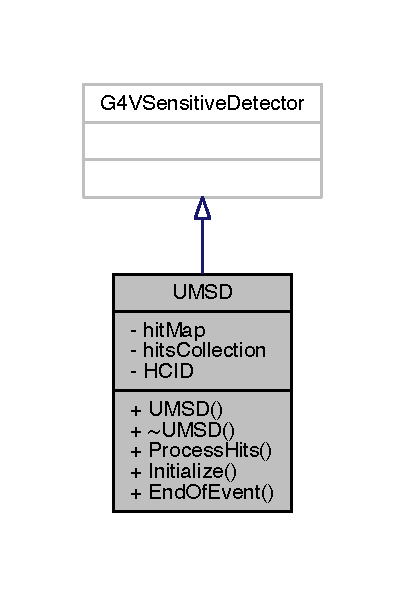
\includegraphics[width=194pt]{classUMSD__inherit__graph}
\end{center}
\end{figure}


Collaboration diagram for U\+M\+S\+D\+:
\nopagebreak
\begin{figure}[H]
\begin{center}
\leavevmode
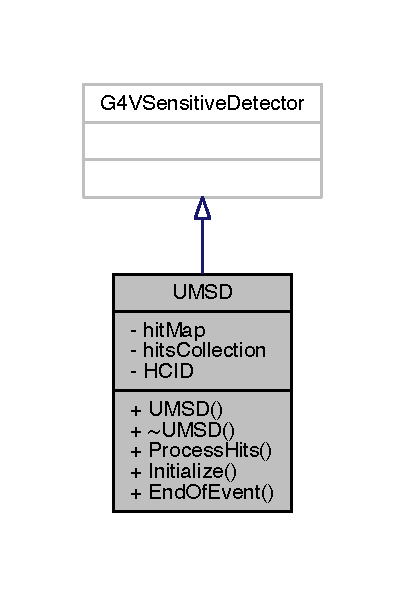
\includegraphics[width=194pt]{classUMSD__coll__graph}
\end{center}
\end{figure}
\subsection*{Public Member Functions}
\begin{DoxyCompactItemize}
\item 
\hyperlink{classUMSD_aba31b29e6b53618650ac627f49e813f8}{U\+M\+S\+D} (G4\+String S\+Dname)
\item 
\hyperlink{classUMSD_a8e9150046d7e00c3179d30c27fb01e26}{$\sim$\+U\+M\+S\+D} ()
\item 
G4bool \hyperlink{classUMSD_afdcb8b2b14fa1e9c22f82d305381849a}{Process\+Hits} (G4\+Step $\ast$step, G4\+Touchable\+History $\ast$R\+Ohist)
\begin{DoxyCompactList}\small\item\em Mandatory class. \end{DoxyCompactList}\item 
void \hyperlink{classUMSD_a15c7a91080ef37306aadec1def3e5acd}{Initialize} (G4\+H\+Cof\+This\+Event $\ast$H\+C\+E)
\item 
void \hyperlink{classUMSD_a62353fbde18e0b32cc1d8ea455c278af}{End\+Of\+Event} (G4\+H\+Cof\+This\+Event $\ast$H\+C\+E)
\begin{DoxyCompactList}\small\item\em defines what happens at the end of each event. \end{DoxyCompactList}\end{DoxyCompactItemize}
\subsection*{Private Types}
\begin{DoxyCompactItemize}
\item 
typedef std\+::map$<$ G4int, \hyperlink{classUMHit}{U\+M\+Hit} $\ast$ $>$ \hyperlink{classUMSD_a6da3356d9e0e0512f26ac3c11cdbb6d8}{hit\+Map\+\_\+t}
\end{DoxyCompactItemize}
\subsection*{Private Attributes}
\begin{DoxyCompactItemize}
\item 
\hyperlink{classUMSD_a6da3356d9e0e0512f26ac3c11cdbb6d8}{hit\+Map\+\_\+t} \hyperlink{classUMSD_acc453bf46c439aec3d5c82715152fab4}{hit\+Map}
\begin{DoxyCompactList}\small\item\em Helper mapping layer number with hit. \end{DoxyCompactList}\item 
\hyperlink{UMHit_8hh_ae4ae3db383f3d522b08825b4ecbfc3e6}{U\+M\+Hits\+Collection} $\ast$ \hyperlink{classUMSD_a6b2f2c42a6be884619371760d8b8752d}{hits\+Collection}
\item 
G4int \hyperlink{classUMSD_a639c42664519bddf251bd758ebc09635}{H\+C\+I\+D}
\begin{DoxyCompactList}\small\item\em Collection of hits in the gas. \end{DoxyCompactList}\end{DoxyCompactItemize}


\subsection{Detailed Description}
Defines the S\+D of the detector construction stores the hits in the Hit Collection of this Event. 

\subsection{Member Typedef Documentation}
\hypertarget{classUMSD_a6da3356d9e0e0512f26ac3c11cdbb6d8}{}\index{U\+M\+S\+D@{U\+M\+S\+D}!hit\+Map\+\_\+t@{hit\+Map\+\_\+t}}
\index{hit\+Map\+\_\+t@{hit\+Map\+\_\+t}!U\+M\+S\+D@{U\+M\+S\+D}}
\subsubsection[{hit\+Map\+\_\+t}]{\setlength{\rightskip}{0pt plus 5cm}typedef std\+::map$<$G4int,{\bf U\+M\+Hit}$\ast$$>$ {\bf U\+M\+S\+D\+::hit\+Map\+\_\+t}\hspace{0.3cm}{\ttfamily [private]}}\label{classUMSD_a6da3356d9e0e0512f26ac3c11cdbb6d8}


\subsection{Constructor \& Destructor Documentation}
\hypertarget{classUMSD_aba31b29e6b53618650ac627f49e813f8}{}\index{U\+M\+S\+D@{U\+M\+S\+D}!U\+M\+S\+D@{U\+M\+S\+D}}
\index{U\+M\+S\+D@{U\+M\+S\+D}!U\+M\+S\+D@{U\+M\+S\+D}}
\subsubsection[{U\+M\+S\+D(\+G4\+String S\+Dname)}]{\setlength{\rightskip}{0pt plus 5cm}U\+M\+S\+D\+::\+U\+M\+S\+D (
\begin{DoxyParamCaption}
\item[{G4\+String}]{S\+Dname}
\end{DoxyParamCaption}
)}\label{classUMSD_aba31b29e6b53618650ac627f49e813f8}
Source for the \begin{DoxySeeAlso}{See also}
U\+M\+Sensitive\+Detector
\end{DoxySeeAlso}
\begin{DoxyAuthor}{Author}
Nikolaos Karastathis $<$ nkarast .at. cern .dot. ch $>$ 
\end{DoxyAuthor}
\begin{DoxyVersion}{Version}
v2.\+0 
\end{DoxyVersion}
\{\textquotesingle{}collection\+Name\textquotesingle{} is a protected data member of base class G4\+V\+Sensitive\+Detector. Here we declare the name of the collection we will be using.\}

\{Note that we may add as many collection names we would wish\+: ie \hypertarget{classUMSD_a8e9150046d7e00c3179d30c27fb01e26}{}\index{U\+M\+S\+D@{U\+M\+S\+D}!````~U\+M\+S\+D@{$\sim$\+U\+M\+S\+D}}
\index{````~U\+M\+S\+D@{$\sim$\+U\+M\+S\+D}!U\+M\+S\+D@{U\+M\+S\+D}}
\subsubsection[{$\sim$\+U\+M\+S\+D()}]{\setlength{\rightskip}{0pt plus 5cm}U\+M\+S\+D\+::$\sim$\+U\+M\+S\+D (
\begin{DoxyParamCaption}
{}
\end{DoxyParamCaption}
)\hspace{0.3cm}{\ttfamily [inline]}}\label{classUMSD_a8e9150046d7e00c3179d30c27fb01e26}


\subsection{Member Function Documentation}
\hypertarget{classUMSD_a62353fbde18e0b32cc1d8ea455c278af}{}\index{U\+M\+S\+D@{U\+M\+S\+D}!End\+Of\+Event@{End\+Of\+Event}}
\index{End\+Of\+Event@{End\+Of\+Event}!U\+M\+S\+D@{U\+M\+S\+D}}
\subsubsection[{End\+Of\+Event(\+G4\+H\+Cof\+This\+Event $\ast$\+H\+C\+E)}]{\setlength{\rightskip}{0pt plus 5cm}void U\+M\+S\+D\+::\+End\+Of\+Event (
\begin{DoxyParamCaption}
\item[{G4\+H\+Cof\+This\+Event $\ast$}]{H\+C\+E}
\end{DoxyParamCaption}
)}\label{classUMSD_a62353fbde18e0b32cc1d8ea455c278af}


defines what happens at the end of each event. 

do nothing -\/

\begin{DoxySeeAlso}{See also}
End\+Of\+Event\+Action will take care of that 
\end{DoxySeeAlso}
\hypertarget{classUMSD_a15c7a91080ef37306aadec1def3e5acd}{}\index{U\+M\+S\+D@{U\+M\+S\+D}!Initialize@{Initialize}}
\index{Initialize@{Initialize}!U\+M\+S\+D@{U\+M\+S\+D}}
\subsubsection[{Initialize(\+G4\+H\+Cof\+This\+Event $\ast$\+H\+C\+E)}]{\setlength{\rightskip}{0pt plus 5cm}void U\+M\+S\+D\+::\+Initialize (
\begin{DoxyParamCaption}
\item[{G4\+H\+Cof\+This\+Event $\ast$}]{H\+C\+E}
\end{DoxyParamCaption}
)}\label{classUMSD_a15c7a91080ef37306aadec1def3e5acd}
To insert the collection, we need to get an index for it. This index is unique to the collection. It is provided by the Get\+Collection\+I\+D(...) method (which calls what is needed in the kernel to get this index). \hypertarget{classUMSD_afdcb8b2b14fa1e9c22f82d305381849a}{}\index{U\+M\+S\+D@{U\+M\+S\+D}!Process\+Hits@{Process\+Hits}}
\index{Process\+Hits@{Process\+Hits}!U\+M\+S\+D@{U\+M\+S\+D}}
\subsubsection[{Process\+Hits(\+G4\+Step $\ast$step, G4\+Touchable\+History $\ast$\+R\+Ohist)}]{\setlength{\rightskip}{0pt plus 5cm}G4bool U\+M\+S\+D\+::\+Process\+Hits (
\begin{DoxyParamCaption}
\item[{G4\+Step $\ast$}]{step, }
\item[{G4\+Touchable\+History $\ast$}]{R\+Ohist}
\end{DoxyParamCaption}
)}\label{classUMSD_afdcb8b2b14fa1e9c22f82d305381849a}


Mandatory class. 

Get the track for the step

Generate the info for this track (position, energy, particle, etc)

Generate a new \hyperlink{classUMHit}{U\+M\+Hit} and store the information

then insert the hit into the Hits Collection 

\subsection{Field Documentation}
\hypertarget{classUMSD_a639c42664519bddf251bd758ebc09635}{}\index{U\+M\+S\+D@{U\+M\+S\+D}!H\+C\+I\+D@{H\+C\+I\+D}}
\index{H\+C\+I\+D@{H\+C\+I\+D}!U\+M\+S\+D@{U\+M\+S\+D}}
\subsubsection[{H\+C\+I\+D}]{\setlength{\rightskip}{0pt plus 5cm}G4int U\+M\+S\+D\+::\+H\+C\+I\+D\hspace{0.3cm}{\ttfamily [private]}}\label{classUMSD_a639c42664519bddf251bd758ebc09635}


Collection of hits in the gas. 

\hypertarget{classUMSD_acc453bf46c439aec3d5c82715152fab4}{}\index{U\+M\+S\+D@{U\+M\+S\+D}!hit\+Map@{hit\+Map}}
\index{hit\+Map@{hit\+Map}!U\+M\+S\+D@{U\+M\+S\+D}}
\subsubsection[{hit\+Map}]{\setlength{\rightskip}{0pt plus 5cm}{\bf hit\+Map\+\_\+t} U\+M\+S\+D\+::hit\+Map\hspace{0.3cm}{\ttfamily [private]}}\label{classUMSD_acc453bf46c439aec3d5c82715152fab4}


Helper mapping layer number with hit. 

\hypertarget{classUMSD_a6b2f2c42a6be884619371760d8b8752d}{}\index{U\+M\+S\+D@{U\+M\+S\+D}!hits\+Collection@{hits\+Collection}}
\index{hits\+Collection@{hits\+Collection}!U\+M\+S\+D@{U\+M\+S\+D}}
\subsubsection[{hits\+Collection}]{\setlength{\rightskip}{0pt plus 5cm}{\bf U\+M\+Hits\+Collection}$\ast$ U\+M\+S\+D\+::hits\+Collection\hspace{0.3cm}{\ttfamily [private]}}\label{classUMSD_a6b2f2c42a6be884619371760d8b8752d}


The documentation for this class was generated from the following files\+:\begin{DoxyCompactItemize}
\item 
include/\hyperlink{UMSD_8hh}{U\+M\+S\+D.\+hh}\item 
src/\hyperlink{UMSD_8cc}{U\+M\+S\+D.\+cc}\end{DoxyCompactItemize}

\chapter{File Documentation}
\hypertarget{PhysListEmStandard_8hh}{}\section{include/\+Phys\+List\+Em\+Standard.hh File Reference}
\label{PhysListEmStandard_8hh}\index{include/\+Phys\+List\+Em\+Standard.\+hh@{include/\+Phys\+List\+Em\+Standard.\+hh}}
{\ttfamily \#include \char`\"{}G4\+V\+Physics\+Constructor.\+hh\char`\"{}}\\*
{\ttfamily \#include \char`\"{}globals.\+hh\char`\"{}}\\*
{\ttfamily \#include \char`\"{}G4\+Physical\+Constants.\+hh\char`\"{}}\\*
{\ttfamily \#include \char`\"{}G4\+System\+Of\+Units.\+hh\char`\"{}}\\*
Include dependency graph for Phys\+List\+Em\+Standard.\+hh\+:
\nopagebreak
\begin{figure}[H]
\begin{center}
\leavevmode
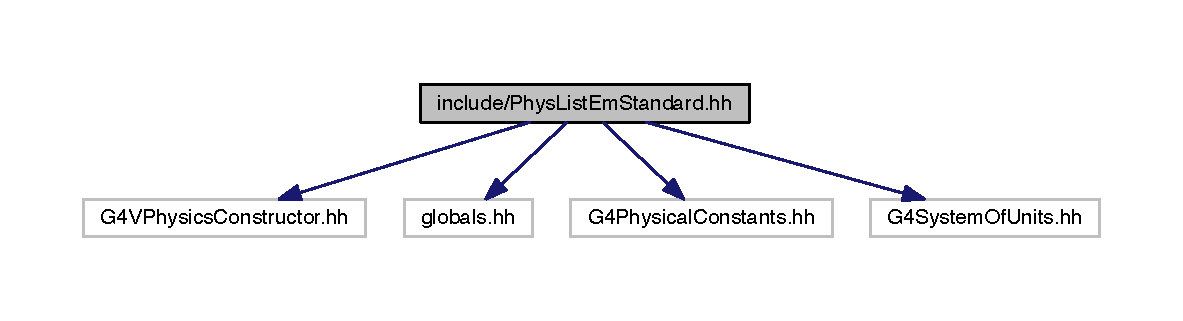
\includegraphics[width=350pt]{PhysListEmStandard_8hh__incl}
\end{center}
\end{figure}
This graph shows which files directly or indirectly include this file\+:
\nopagebreak
\begin{figure}[H]
\begin{center}
\leavevmode
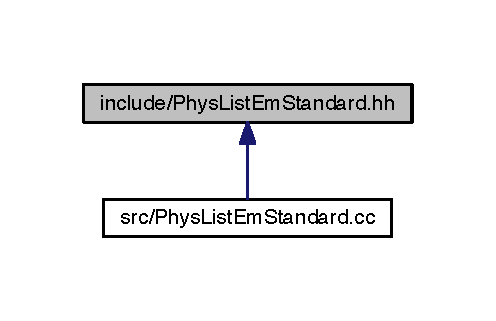
\includegraphics[width=238pt]{PhysListEmStandard_8hh__dep__incl}
\end{center}
\end{figure}
\subsection*{Data Structures}
\begin{DoxyCompactItemize}
\item 
class \hyperlink{classPhysListEmStandard}{Phys\+List\+Em\+Standard}
\end{DoxyCompactItemize}

\hypertarget{RunAction_8hh}{}\section{include/\+Run\+Action.hh File Reference}
\label{RunAction_8hh}\index{include/\+Run\+Action.\+hh@{include/\+Run\+Action.\+hh}}
{\ttfamily \#include \char`\"{}G4\+User\+Run\+Action.\+hh\char`\"{}}\\*
{\ttfamily \#include \char`\"{}T\+File.\+h\char`\"{}}\\*
{\ttfamily \#include \char`\"{}T\+H1\+F.\+h\char`\"{}}\\*
{\ttfamily \#include \char`\"{}T\+Tree.\+h\char`\"{}}\\*
{\ttfamily \#include \char`\"{}U\+M\+Root\+Saver.\+hh\char`\"{}}\\*
{\ttfamily \#include \char`\"{}G4\+Physical\+Constants.\+hh\char`\"{}}\\*
{\ttfamily \#include \char`\"{}G4\+System\+Of\+Units.\+hh\char`\"{}}\\*
{\ttfamily \#include $<$fstream$>$}\\*
Include dependency graph for Run\+Action.\+hh\+:
\nopagebreak
\begin{figure}[H]
\begin{center}
\leavevmode
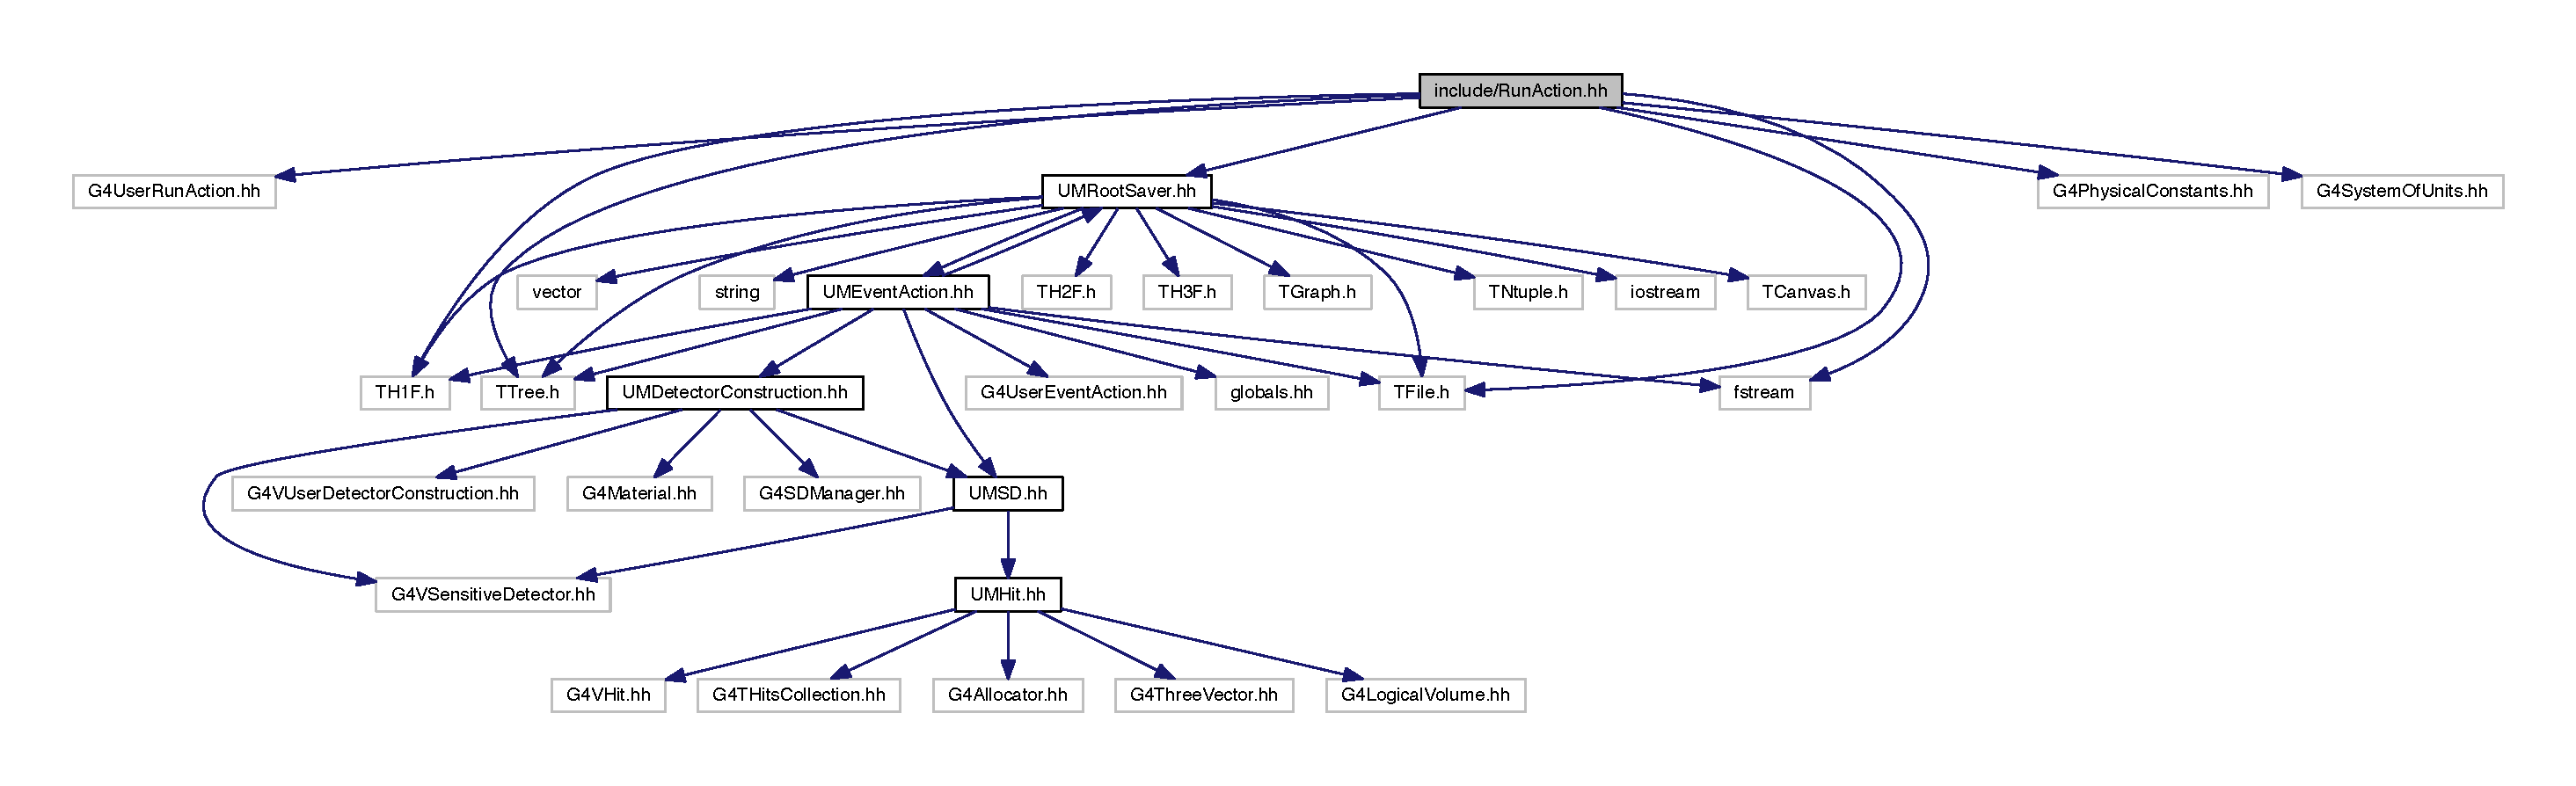
\includegraphics[width=350pt]{RunAction_8hh__incl}
\end{center}
\end{figure}
This graph shows which files directly or indirectly include this file\+:
\nopagebreak
\begin{figure}[H]
\begin{center}
\leavevmode
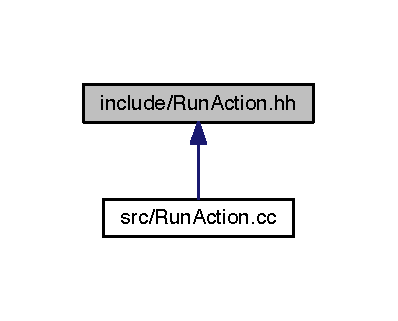
\includegraphics[width=191pt]{RunAction_8hh__dep__incl}
\end{center}
\end{figure}
\subsection*{Data Structures}
\begin{DoxyCompactItemize}
\item 
class \hyperlink{classRunAction}{Run\+Action}
\begin{DoxyCompactList}\small\item\em The user-\/defined Run action class At the. \end{DoxyCompactList}\end{DoxyCompactItemize}

\hypertarget{UMConfig_8hh}{}\section{include/\+U\+M\+Config.hh File Reference}
\label{UMConfig_8hh}\index{include/\+U\+M\+Config.\+hh@{include/\+U\+M\+Config.\+hh}}
{\ttfamily \#include \char`\"{}G4\+Physical\+Constants.\+hh\char`\"{}}\\*
{\ttfamily \#include \char`\"{}G4\+System\+Of\+Units.\+hh\char`\"{}}\\*
{\ttfamily \#include \char`\"{}globals.\+hh\char`\"{}}\\*
Include dependency graph for U\+M\+Config.\+hh\+:
\nopagebreak
\begin{figure}[H]
\begin{center}
\leavevmode
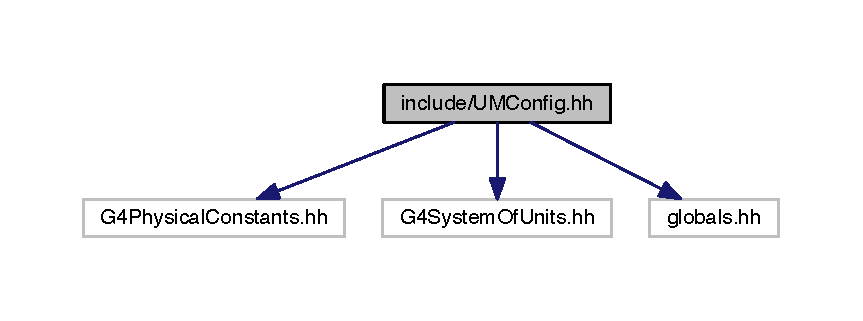
\includegraphics[width=350pt]{UMConfig_8hh__incl}
\end{center}
\end{figure}
This graph shows which files directly or indirectly include this file\+:
\nopagebreak
\begin{figure}[H]
\begin{center}
\leavevmode
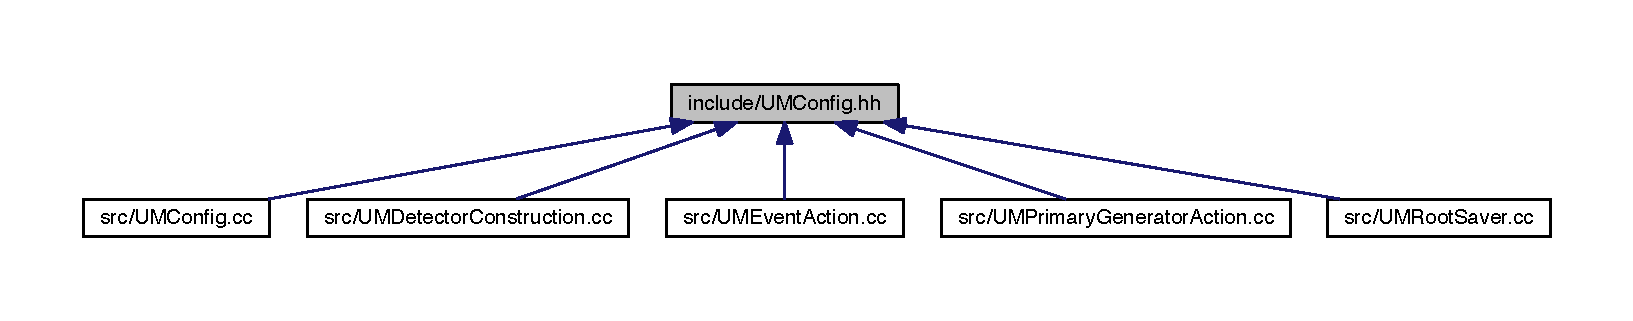
\includegraphics[width=350pt]{UMConfig_8hh__dep__incl}
\end{center}
\end{figure}
\subsection*{Data Structures}
\begin{DoxyCompactItemize}
\item 
struct \hyperlink{structUMConfig}{U\+M\+Config}
\end{DoxyCompactItemize}

\hypertarget{UMDetectorConstruction_8hh}{}\section{include/\+U\+M\+Detector\+Construction.hh File Reference}
\label{UMDetectorConstruction_8hh}\index{include/\+U\+M\+Detector\+Construction.\+hh@{include/\+U\+M\+Detector\+Construction.\+hh}}
{\ttfamily \#include \char`\"{}G4\+V\+User\+Detector\+Construction.\+hh\char`\"{}}\\*
{\ttfamily \#include \char`\"{}G4\+Material.\+hh\char`\"{}}\\*
{\ttfamily \#include \char`\"{}G4\+S\+D\+Manager.\+hh\char`\"{}}\\*
{\ttfamily \#include \char`\"{}G4\+V\+Sensitive\+Detector.\+hh\char`\"{}}\\*
{\ttfamily \#include \char`\"{}U\+M\+S\+D.\+hh\char`\"{}}\\*
Include dependency graph for U\+M\+Detector\+Construction.\+hh\+:
\nopagebreak
\begin{figure}[H]
\begin{center}
\leavevmode
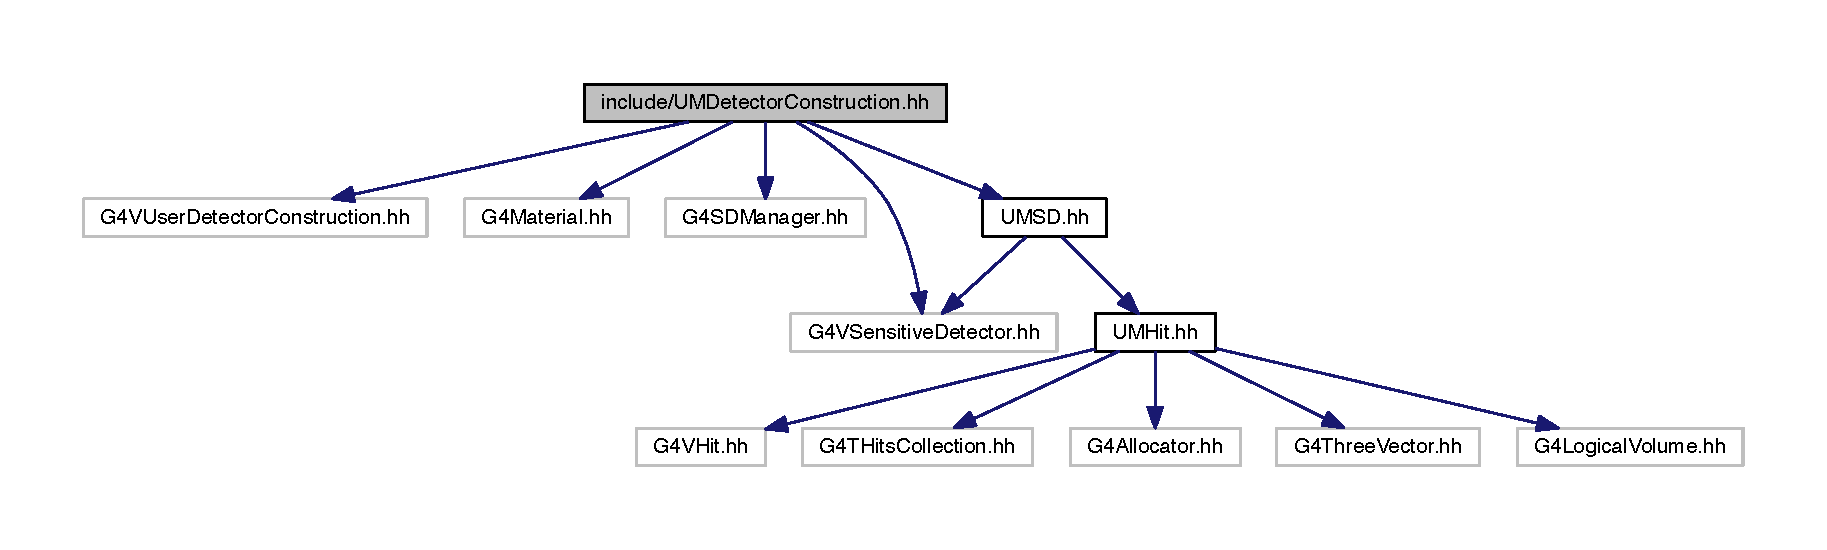
\includegraphics[width=350pt]{UMDetectorConstruction_8hh__incl}
\end{center}
\end{figure}
This graph shows which files directly or indirectly include this file\+:
\nopagebreak
\begin{figure}[H]
\begin{center}
\leavevmode
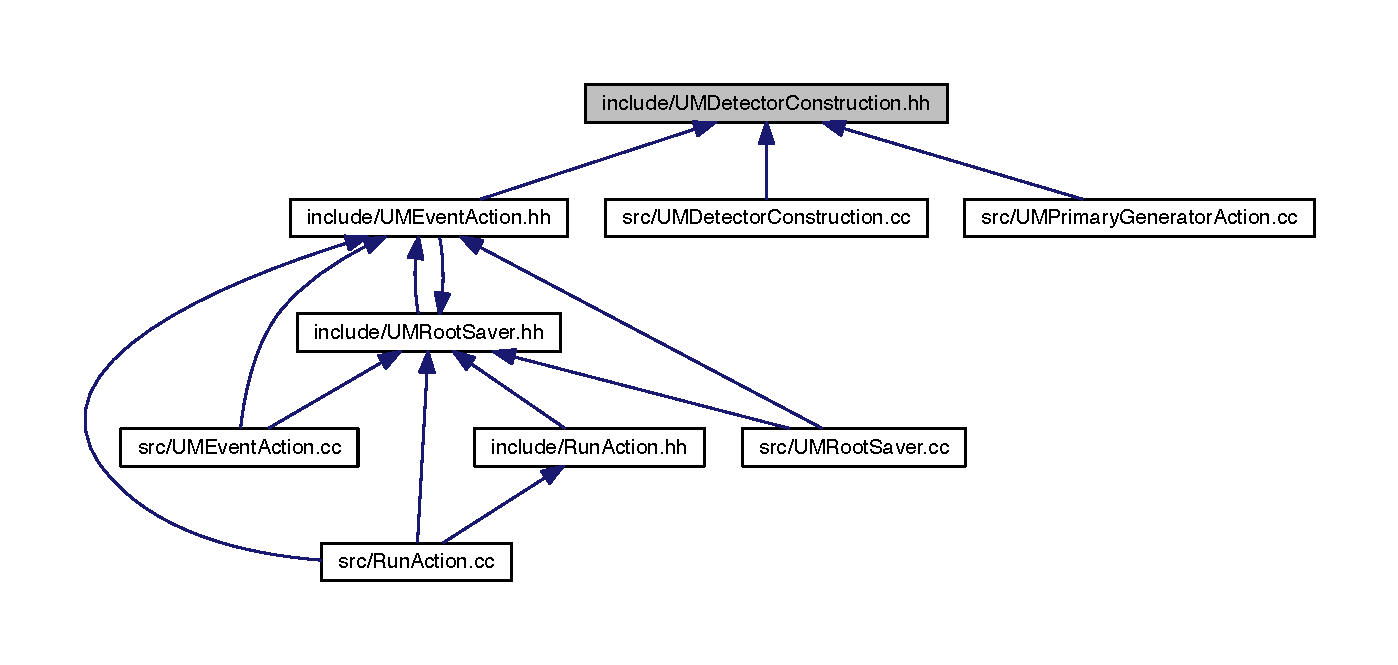
\includegraphics[width=350pt]{UMDetectorConstruction_8hh__dep__incl}
\end{center}
\end{figure}
\subsection*{Data Structures}
\begin{DoxyCompactItemize}
\item 
class \hyperlink{classUMDetectorConstruction}{U\+M\+Detector\+Construction}
\end{DoxyCompactItemize}

\hypertarget{UMEventAction_8hh}{}\section{include/\+U\+M\+Event\+Action.hh File Reference}
\label{UMEventAction_8hh}\index{include/\+U\+M\+Event\+Action.\+hh@{include/\+U\+M\+Event\+Action.\+hh}}
{\ttfamily \#include \char`\"{}U\+M\+Detector\+Construction.\+hh\char`\"{}}\\*
{\ttfamily \#include \char`\"{}U\+M\+S\+D.\+hh\char`\"{}}\\*
{\ttfamily \#include \char`\"{}U\+M\+Root\+Saver.\+hh\char`\"{}}\\*
{\ttfamily \#include \char`\"{}G4\+User\+Event\+Action.\+hh\char`\"{}}\\*
{\ttfamily \#include \char`\"{}globals.\+hh\char`\"{}}\\*
{\ttfamily \#include \char`\"{}T\+H1\+F.\+h\char`\"{}}\\*
{\ttfamily \#include \char`\"{}T\+File.\+h\char`\"{}}\\*
{\ttfamily \#include \char`\"{}T\+Tree.\+h\char`\"{}}\\*
{\ttfamily \#include $<$fstream$>$}\\*
Include dependency graph for U\+M\+Event\+Action.\+hh\+:
\nopagebreak
\begin{figure}[H]
\begin{center}
\leavevmode
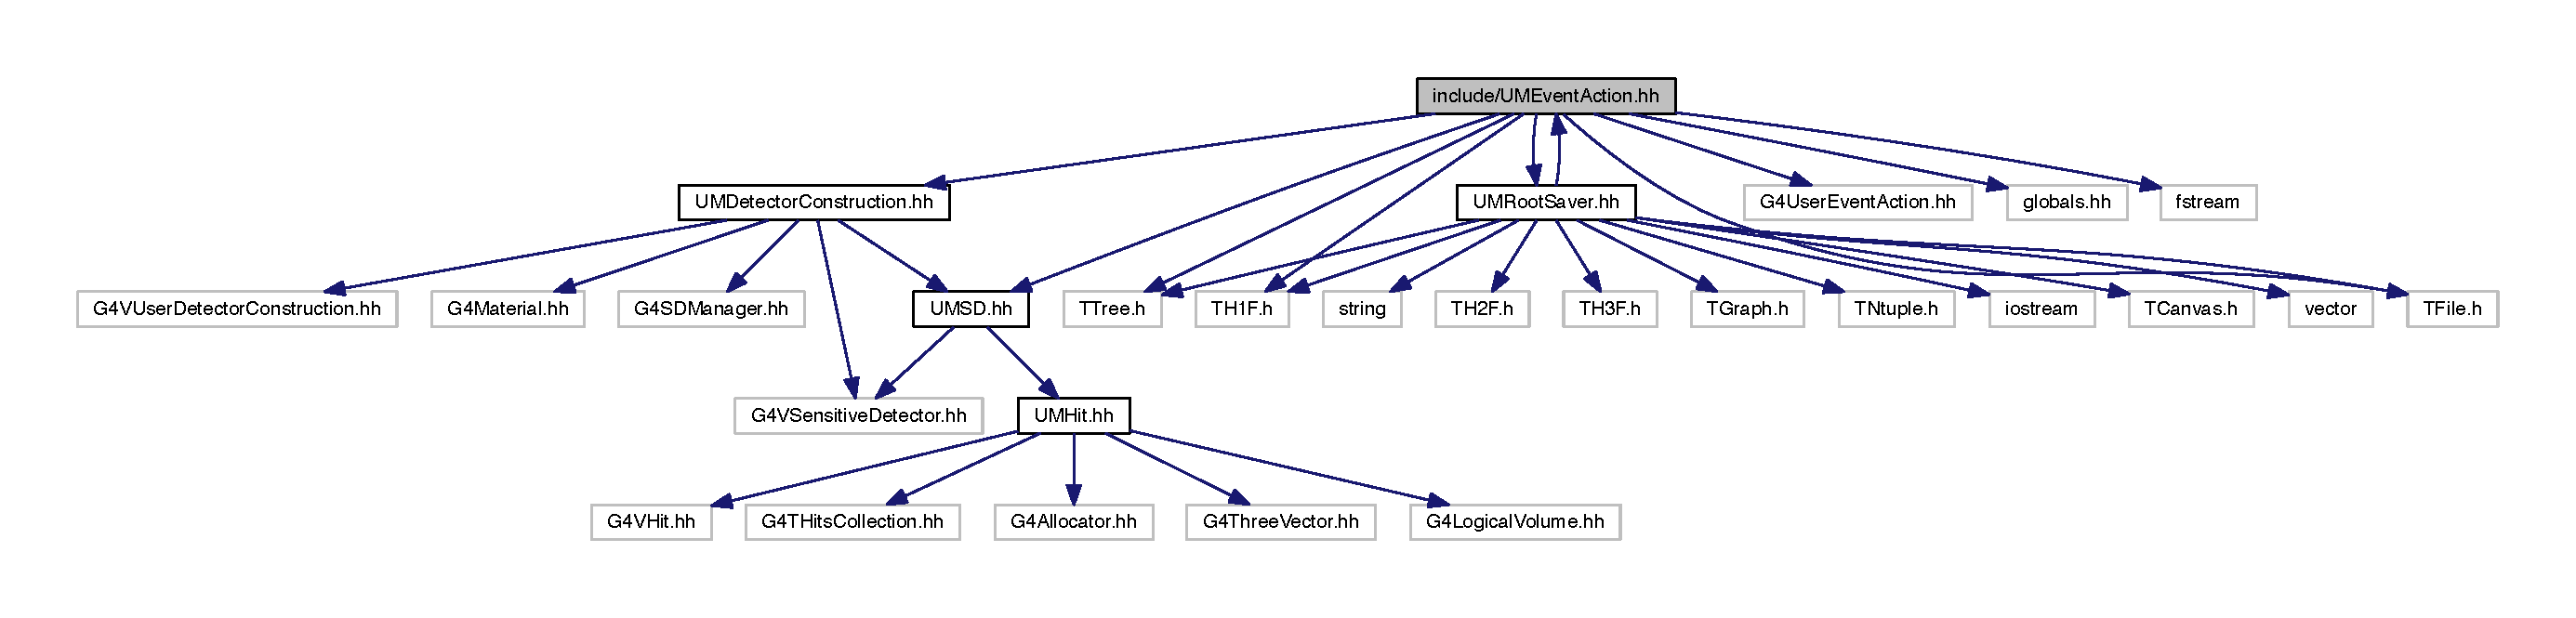
\includegraphics[width=350pt]{UMEventAction_8hh__incl}
\end{center}
\end{figure}
This graph shows which files directly or indirectly include this file\+:
\nopagebreak
\begin{figure}[H]
\begin{center}
\leavevmode
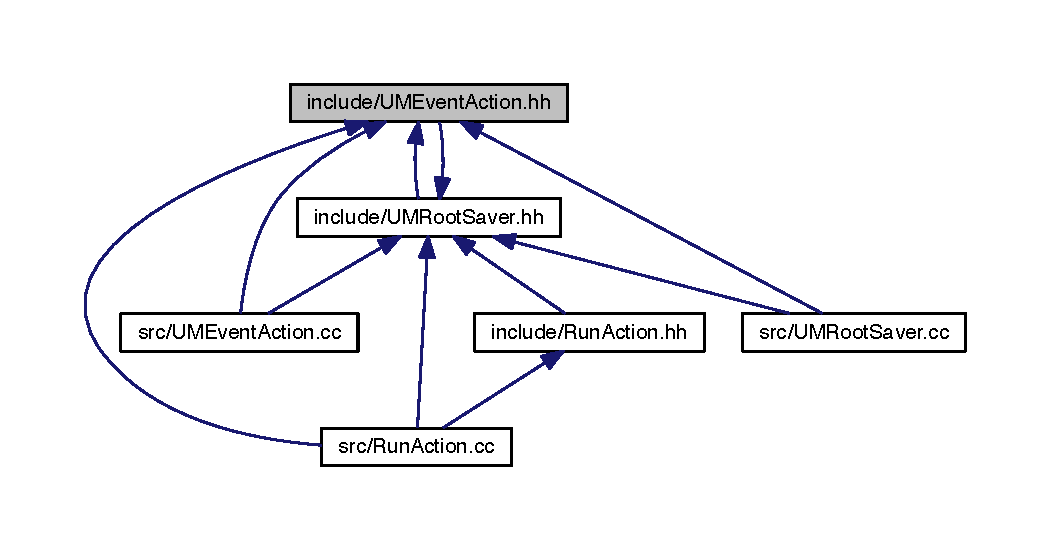
\includegraphics[width=350pt]{UMEventAction_8hh__dep__incl}
\end{center}
\end{figure}
\subsection*{Data Structures}
\begin{DoxyCompactItemize}
\item 
class \hyperlink{classUMEventAction}{U\+M\+Event\+Action}
\end{DoxyCompactItemize}

\hypertarget{UMHit_8hh}{}\section{include/\+U\+M\+Hit.hh File Reference}
\label{UMHit_8hh}\index{include/\+U\+M\+Hit.\+hh@{include/\+U\+M\+Hit.\+hh}}
{\ttfamily \#include \char`\"{}G4\+V\+Hit.\+hh\char`\"{}}\\*
{\ttfamily \#include \char`\"{}G4\+T\+Hits\+Collection.\+hh\char`\"{}}\\*
{\ttfamily \#include \char`\"{}G4\+Allocator.\+hh\char`\"{}}\\*
{\ttfamily \#include \char`\"{}G4\+Three\+Vector.\+hh\char`\"{}}\\*
{\ttfamily \#include \char`\"{}G4\+Logical\+Volume.\+hh\char`\"{}}\\*
Include dependency graph for U\+M\+Hit.\+hh\+:
\nopagebreak
\begin{figure}[H]
\begin{center}
\leavevmode
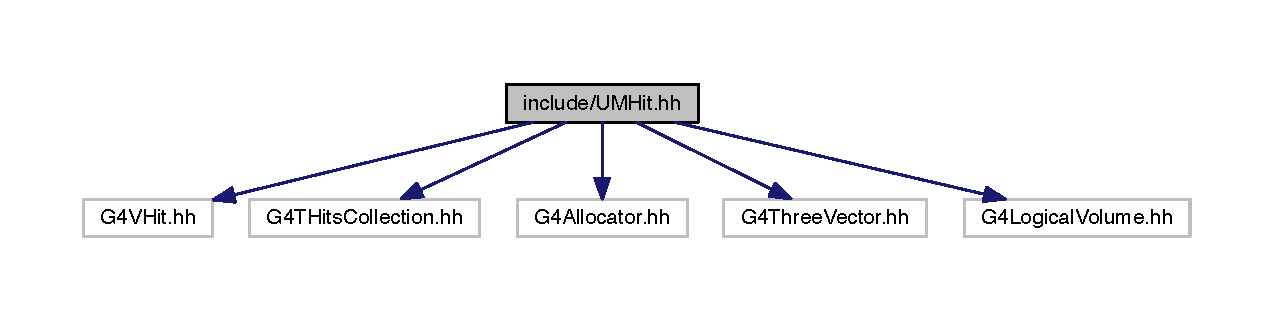
\includegraphics[width=350pt]{UMHit_8hh__incl}
\end{center}
\end{figure}
This graph shows which files directly or indirectly include this file\+:
\nopagebreak
\begin{figure}[H]
\begin{center}
\leavevmode
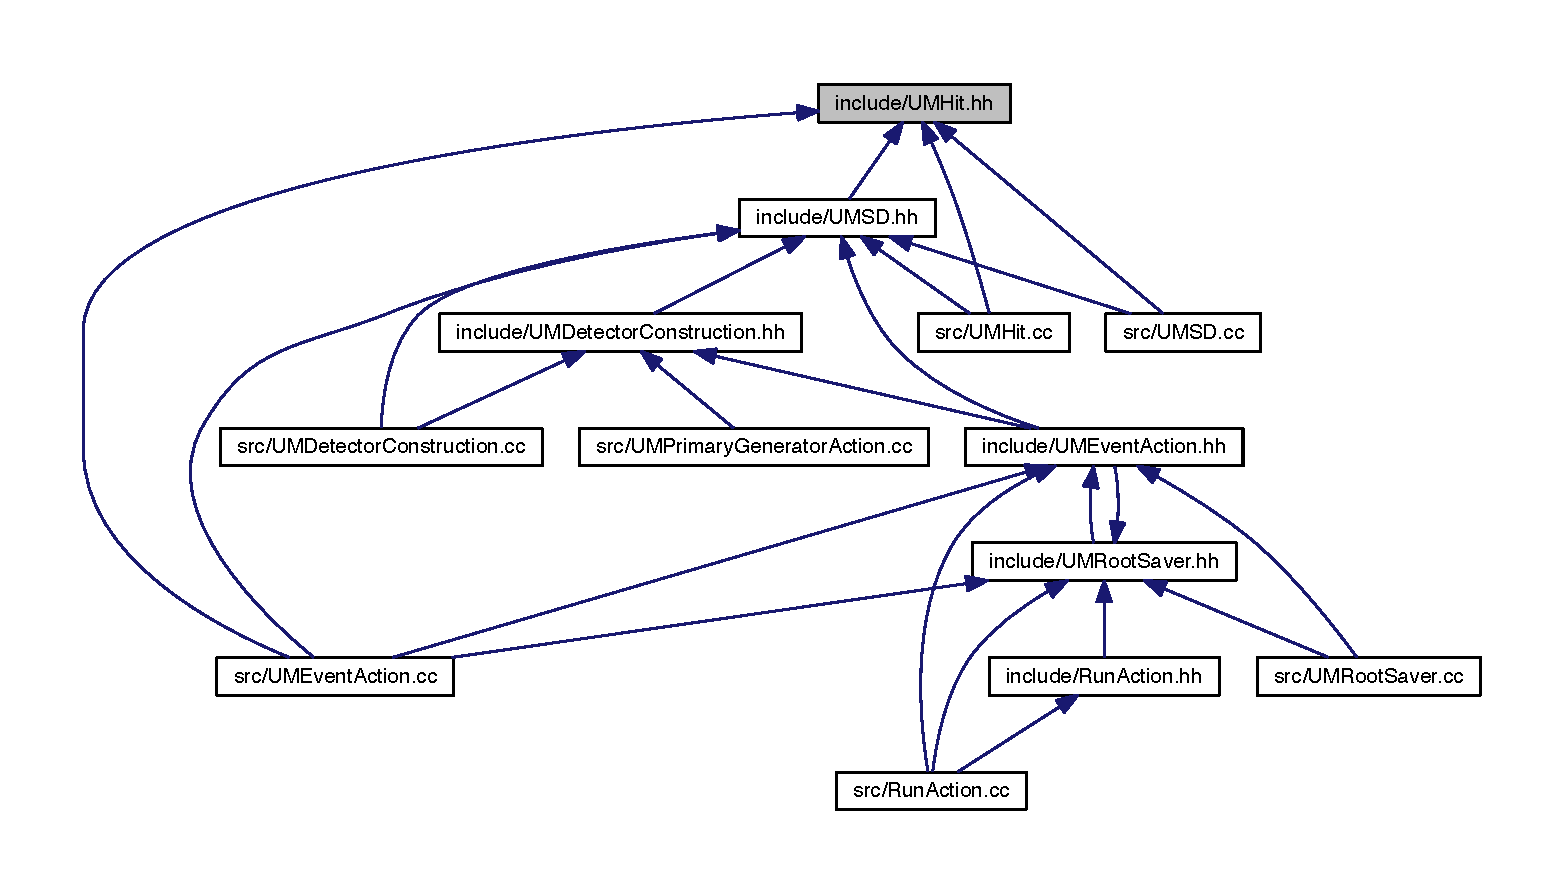
\includegraphics[width=350pt]{UMHit_8hh__dep__incl}
\end{center}
\end{figure}
\subsection*{Data Structures}
\begin{DoxyCompactItemize}
\item 
class \hyperlink{classUMHit}{U\+M\+Hit}
\end{DoxyCompactItemize}
\subsection*{Typedefs}
\begin{DoxyCompactItemize}
\item 
typedef G4\+T\+Hits\+Collection$<$ \hyperlink{classUMHit}{U\+M\+Hit} $>$ \hyperlink{UMHit_8hh_ae4ae3db383f3d522b08825b4ecbfc3e6}{U\+M\+Hits\+Collection}
\begin{DoxyCompactList}\small\item\em Define the \char`\"{}hit collection\char`\"{} using the template class G4\+T\+Hits\+Collection\+: \end{DoxyCompactList}\end{DoxyCompactItemize}
\subsection*{Variables}
\begin{DoxyCompactItemize}
\item 
G4\+Allocator$<$ \hyperlink{classUMHit}{U\+M\+Hit} $>$ \hyperlink{UMHit_8hh_a9d8361bd2d8e805dd16550d0d0808c57}{U\+M\+Hit\+Allocator}
\begin{DoxyCompactList}\small\item\em new and delete overloaded operators\+: \end{DoxyCompactList}\end{DoxyCompactItemize}


\subsection{Typedef Documentation}
\hypertarget{UMHit_8hh_ae4ae3db383f3d522b08825b4ecbfc3e6}{}\index{U\+M\+Hit.\+hh@{U\+M\+Hit.\+hh}!U\+M\+Hits\+Collection@{U\+M\+Hits\+Collection}}
\index{U\+M\+Hits\+Collection@{U\+M\+Hits\+Collection}!U\+M\+Hit.\+hh@{U\+M\+Hit.\+hh}}
\subsubsection[{U\+M\+Hits\+Collection}]{\setlength{\rightskip}{0pt plus 5cm}typedef G4\+T\+Hits\+Collection$<${\bf U\+M\+Hit}$>$ {\bf U\+M\+Hits\+Collection}}\label{UMHit_8hh_ae4ae3db383f3d522b08825b4ecbfc3e6}


Define the \char`\"{}hit collection\char`\"{} using the template class G4\+T\+Hits\+Collection\+: 



\subsection{Variable Documentation}
\hypertarget{UMHit_8hh_a9d8361bd2d8e805dd16550d0d0808c57}{}\index{U\+M\+Hit.\+hh@{U\+M\+Hit.\+hh}!U\+M\+Hit\+Allocator@{U\+M\+Hit\+Allocator}}
\index{U\+M\+Hit\+Allocator@{U\+M\+Hit\+Allocator}!U\+M\+Hit.\+hh@{U\+M\+Hit.\+hh}}
\subsubsection[{U\+M\+Hit\+Allocator}]{\setlength{\rightskip}{0pt plus 5cm}G4\+Allocator$<${\bf U\+M\+Hit}$>$ U\+M\+Hit\+Allocator}\label{UMHit_8hh_a9d8361bd2d8e805dd16550d0d0808c57}


new and delete overloaded operators\+: 


\hypertarget{UMPhysicsList_8hh}{}\section{include/\+U\+M\+Physics\+List.hh File Reference}
\label{UMPhysicsList_8hh}\index{include/\+U\+M\+Physics\+List.\+hh@{include/\+U\+M\+Physics\+List.\+hh}}
{\ttfamily \#include \char`\"{}G4\+V\+Modular\+Physics\+List.\+hh\char`\"{}}\\*
{\ttfamily \#include \char`\"{}G4\+V\+User\+Physics\+List.\+hh\char`\"{}}\\*
{\ttfamily \#include \char`\"{}globals.\+hh\char`\"{}}\\*
Include dependency graph for U\+M\+Physics\+List.\+hh\+:
\nopagebreak
\begin{figure}[H]
\begin{center}
\leavevmode
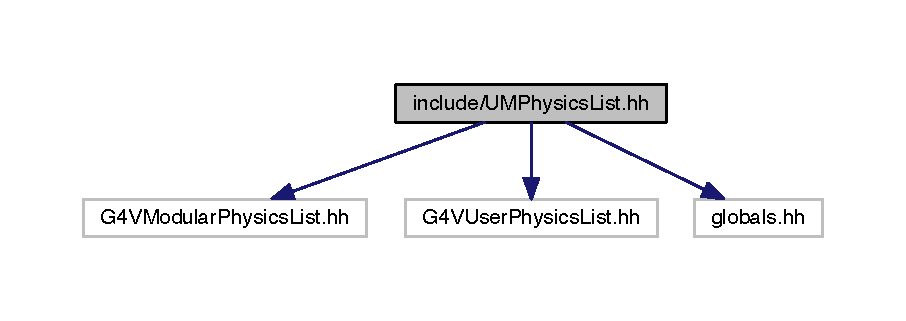
\includegraphics[width=350pt]{UMPhysicsList_8hh__incl}
\end{center}
\end{figure}
This graph shows which files directly or indirectly include this file\+:
\nopagebreak
\begin{figure}[H]
\begin{center}
\leavevmode
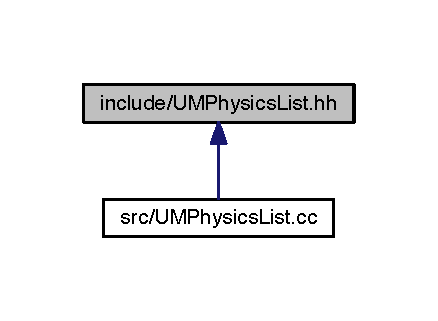
\includegraphics[width=210pt]{UMPhysicsList_8hh__dep__incl}
\end{center}
\end{figure}
\subsection*{Data Structures}
\begin{DoxyCompactItemize}
\item 
class \hyperlink{classUMPhysicsList}{U\+M\+Physics\+List}
\end{DoxyCompactItemize}

\hypertarget{UMPrimaryGeneratorAction_8hh}{}\section{include/\+U\+M\+Primary\+Generator\+Action.hh File Reference}
\label{UMPrimaryGeneratorAction_8hh}\index{include/\+U\+M\+Primary\+Generator\+Action.\+hh@{include/\+U\+M\+Primary\+Generator\+Action.\+hh}}
{\ttfamily \#include \char`\"{}G4\+V\+User\+Primary\+Generator\+Action.\+hh\char`\"{}}\\*
{\ttfamily \#include \char`\"{}globals.\+hh\char`\"{}}\\*
{\ttfamily \#include \char`\"{}G4\+Particle\+Definition.\+hh\char`\"{}}\\*
{\ttfamily \#include \char`\"{}G4\+Physical\+Constants.\+hh\char`\"{}}\\*
{\ttfamily \#include \char`\"{}G4\+System\+Of\+Units.\+hh\char`\"{}}\\*
Include dependency graph for U\+M\+Primary\+Generator\+Action.\+hh\+:
\nopagebreak
\begin{figure}[H]
\begin{center}
\leavevmode
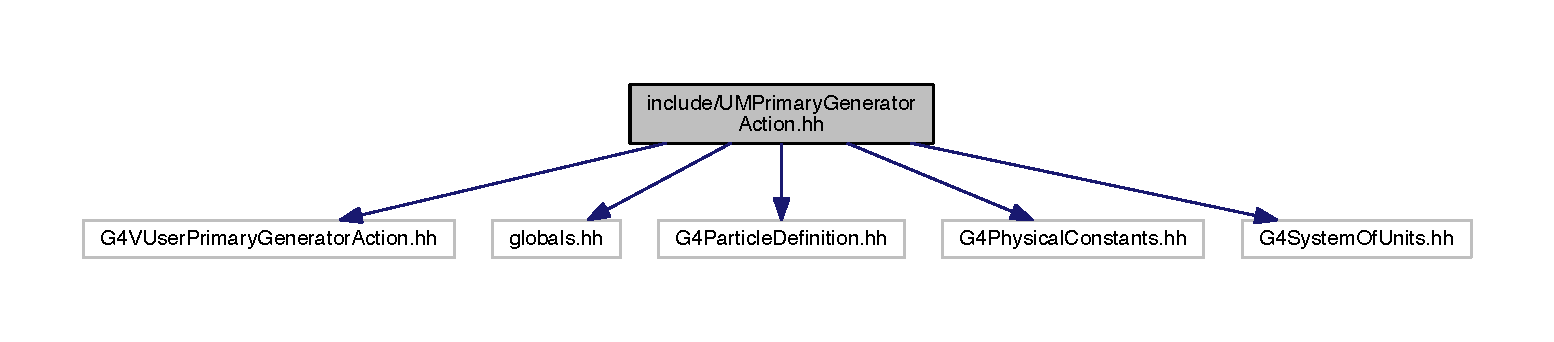
\includegraphics[width=350pt]{UMPrimaryGeneratorAction_8hh__incl}
\end{center}
\end{figure}
This graph shows which files directly or indirectly include this file\+:
\nopagebreak
\begin{figure}[H]
\begin{center}
\leavevmode
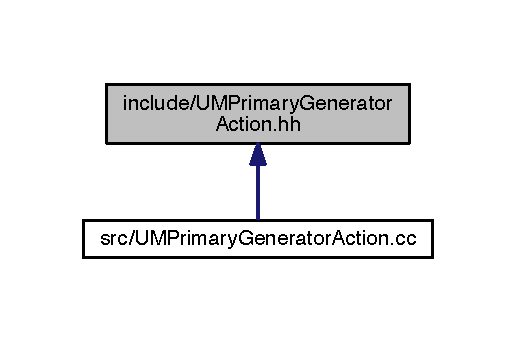
\includegraphics[width=248pt]{UMPrimaryGeneratorAction_8hh__dep__incl}
\end{center}
\end{figure}
\subsection*{Data Structures}
\begin{DoxyCompactItemize}
\item 
class \hyperlink{classUMPrimaryGeneratorAction}{U\+M\+Primary\+Generator\+Action}
\end{DoxyCompactItemize}

\hypertarget{UMRootSaver_8hh}{}\section{include/\+U\+M\+Root\+Saver.hh File Reference}
\label{UMRootSaver_8hh}\index{include/\+U\+M\+Root\+Saver.\+hh@{include/\+U\+M\+Root\+Saver.\+hh}}
{\ttfamily \#include $<$string$>$}\\*
{\ttfamily \#include $<$T\+Tree.\+h$>$}\\*
{\ttfamily \#include $<$T\+H1\+F.\+h$>$}\\*
{\ttfamily \#include $<$T\+H2\+F.\+h$>$}\\*
{\ttfamily \#include $<$T\+H3\+F.\+h$>$}\\*
{\ttfamily \#include $<$T\+File.\+h$>$}\\*
{\ttfamily \#include \char`\"{}T\+Graph.\+h\char`\"{}}\\*
{\ttfamily \#include \char`\"{}U\+M\+Event\+Action.\+hh\char`\"{}}\\*
{\ttfamily \#include \char`\"{}T\+Ntuple.\+h\char`\"{}}\\*
{\ttfamily \#include $<$iostream$>$}\\*
{\ttfamily \#include \char`\"{}T\+Canvas.\+h\char`\"{}}\\*
{\ttfamily \#include $<$vector$>$}\\*
Include dependency graph for U\+M\+Root\+Saver.\+hh\+:
\nopagebreak
\begin{figure}[H]
\begin{center}
\leavevmode
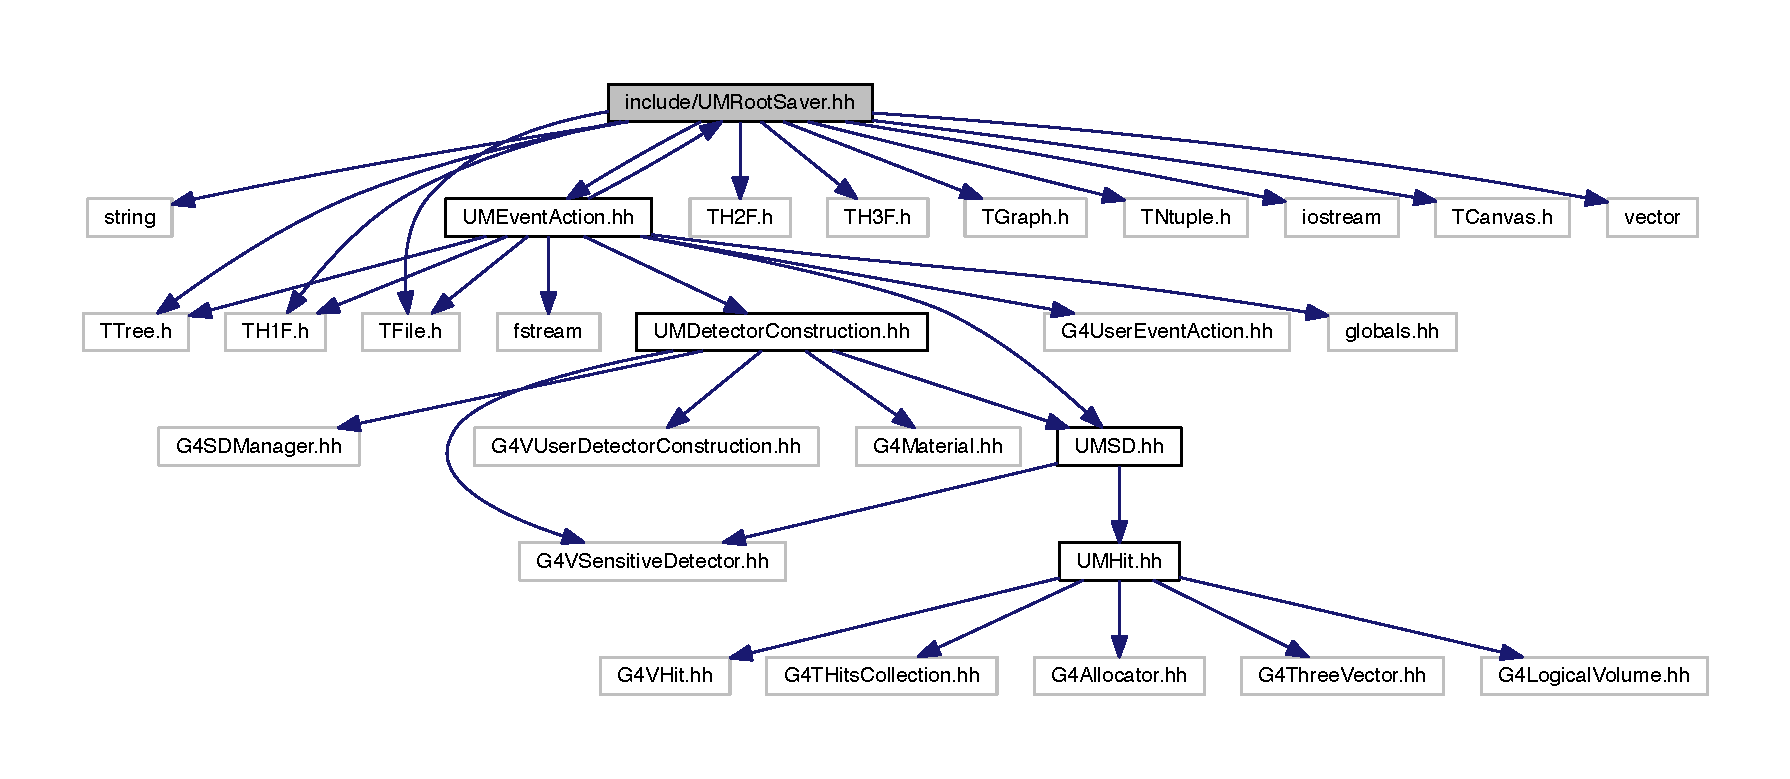
\includegraphics[width=350pt]{UMRootSaver_8hh__incl}
\end{center}
\end{figure}
This graph shows which files directly or indirectly include this file\+:
\nopagebreak
\begin{figure}[H]
\begin{center}
\leavevmode
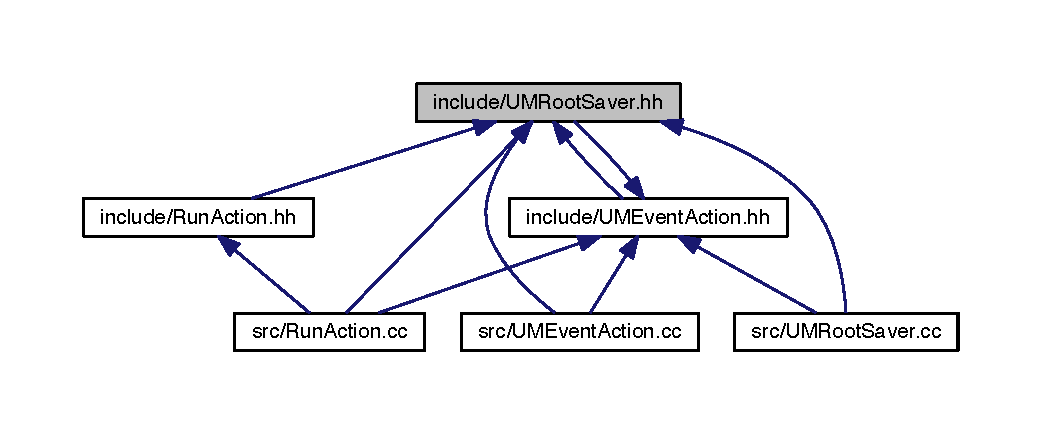
\includegraphics[width=350pt]{UMRootSaver_8hh__dep__incl}
\end{center}
\end{figure}
\subsection*{Data Structures}
\begin{DoxyCompactItemize}
\item 
class \hyperlink{classUMRootSaver}{U\+M\+Root\+Saver}
\end{DoxyCompactItemize}
\subsection*{Variables}
\begin{DoxyCompactItemize}
\item 
double const \hyperlink{UMRootSaver_8hh_af34a60530f8569053554dd583a3a5d94}{Pi} = 3.\+141592
\item 
double const \hyperlink{UMRootSaver_8hh_aca7bc9761c8c10a46efda2d551b32825}{enchannel} =10/1024.
\end{DoxyCompactItemize}


\subsection{Variable Documentation}
\hypertarget{UMRootSaver_8hh_aca7bc9761c8c10a46efda2d551b32825}{}\index{U\+M\+Root\+Saver.\+hh@{U\+M\+Root\+Saver.\+hh}!enchannel@{enchannel}}
\index{enchannel@{enchannel}!U\+M\+Root\+Saver.\+hh@{U\+M\+Root\+Saver.\+hh}}
\subsubsection[{enchannel}]{\setlength{\rightskip}{0pt plus 5cm}double const enchannel =10/1024.}\label{UMRootSaver_8hh_aca7bc9761c8c10a46efda2d551b32825}
\hypertarget{UMRootSaver_8hh_af34a60530f8569053554dd583a3a5d94}{}\index{U\+M\+Root\+Saver.\+hh@{U\+M\+Root\+Saver.\+hh}!Pi@{Pi}}
\index{Pi@{Pi}!U\+M\+Root\+Saver.\+hh@{U\+M\+Root\+Saver.\+hh}}
\subsubsection[{Pi}]{\setlength{\rightskip}{0pt plus 5cm}double const Pi = 3.\+141592}\label{UMRootSaver_8hh_af34a60530f8569053554dd583a3a5d94}

\hypertarget{UMSD_8hh}{}\section{include/\+U\+M\+S\+D.hh File Reference}
\label{UMSD_8hh}\index{include/\+U\+M\+S\+D.\+hh@{include/\+U\+M\+S\+D.\+hh}}
{\ttfamily \#include \char`\"{}G4\+V\+Sensitive\+Detector.\+hh\char`\"{}}\\*
{\ttfamily \#include \char`\"{}U\+M\+Hit.\+hh\char`\"{}}\\*
Include dependency graph for U\+M\+S\+D.\+hh\+:
\nopagebreak
\begin{figure}[H]
\begin{center}
\leavevmode
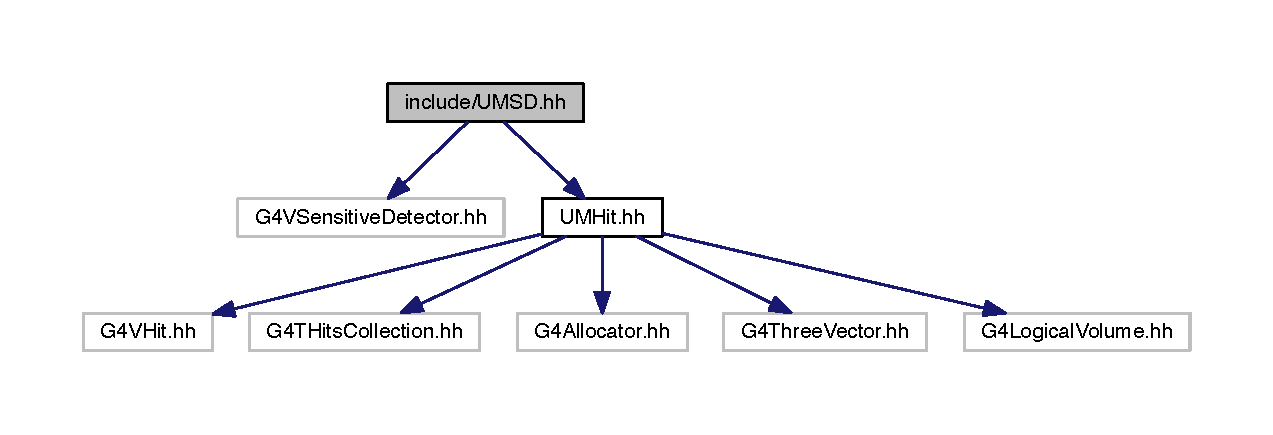
\includegraphics[width=350pt]{UMSD_8hh__incl}
\end{center}
\end{figure}
This graph shows which files directly or indirectly include this file\+:
\nopagebreak
\begin{figure}[H]
\begin{center}
\leavevmode
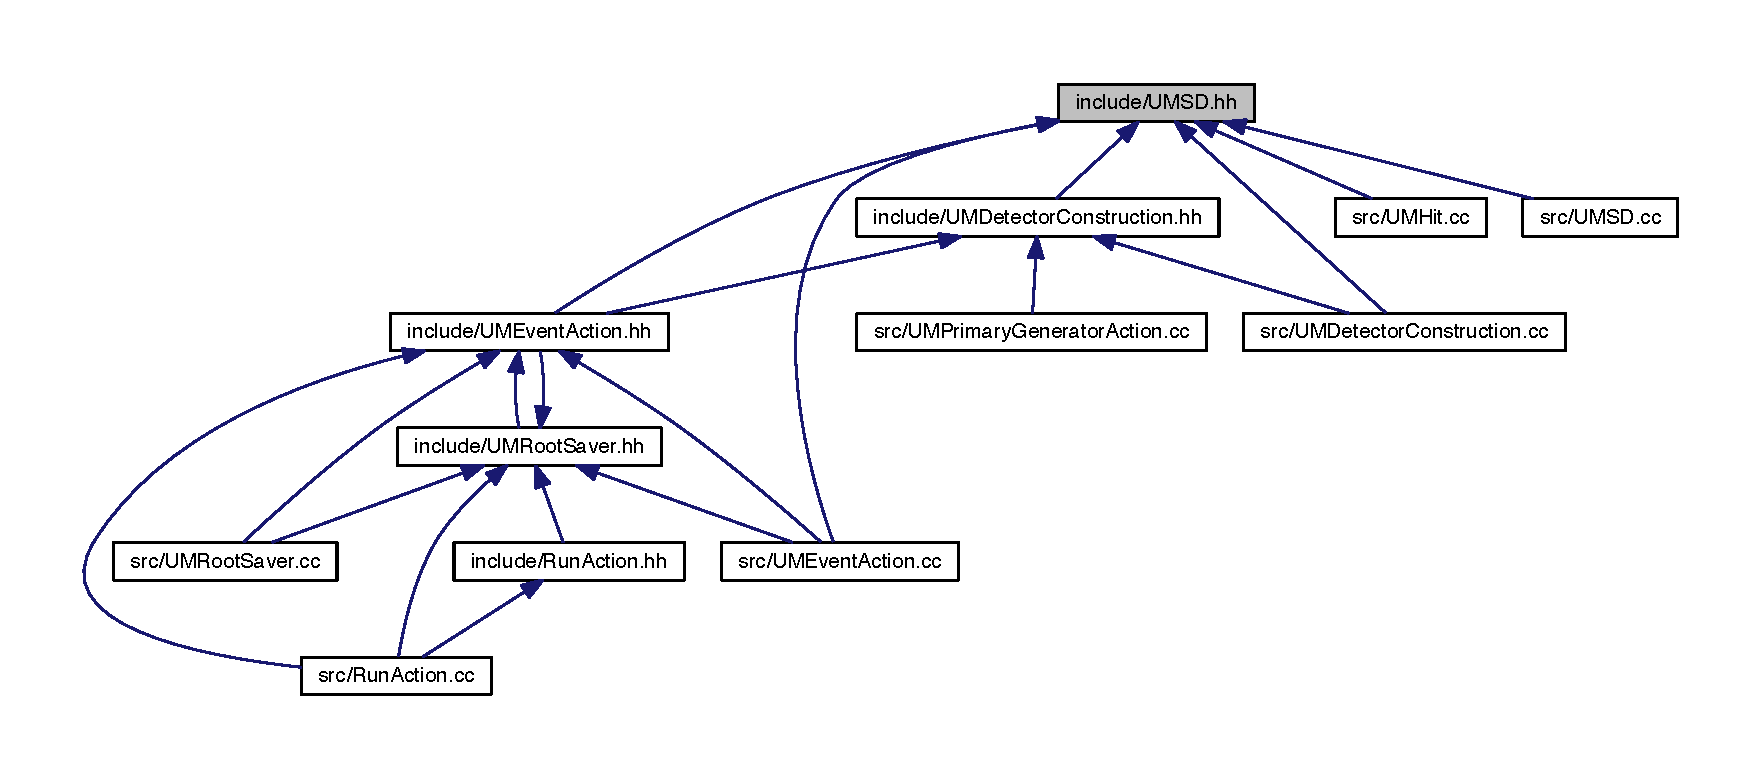
\includegraphics[width=350pt]{UMSD_8hh__dep__incl}
\end{center}
\end{figure}
\subsection*{Data Structures}
\begin{DoxyCompactItemize}
\item 
class \hyperlink{classUMSD}{U\+M\+S\+D}
\end{DoxyCompactItemize}

\hypertarget{UMVisManager_8hh}{}\section{include/\+U\+M\+Vis\+Manager.hh File Reference}
\label{UMVisManager_8hh}\index{include/\+U\+M\+Vis\+Manager.\+hh@{include/\+U\+M\+Vis\+Manager.\+hh}}

\hypertarget{PhysListEmStandard_8cc}{}\section{src/\+Phys\+List\+Em\+Standard.cc File Reference}
\label{PhysListEmStandard_8cc}\index{src/\+Phys\+List\+Em\+Standard.\+cc@{src/\+Phys\+List\+Em\+Standard.\+cc}}
{\ttfamily \#include \char`\"{}Phys\+List\+Em\+Standard.\+hh\char`\"{}}\\*
{\ttfamily \#include \char`\"{}G4\+Particle\+Definition.\+hh\char`\"{}}\\*
{\ttfamily \#include \char`\"{}G4\+Process\+Manager.\+hh\char`\"{}}\\*
{\ttfamily \#include \char`\"{}G4\+Compton\+Scattering.\+hh\char`\"{}}\\*
{\ttfamily \#include \char`\"{}G4\+Gamma\+Conversion.\+hh\char`\"{}}\\*
{\ttfamily \#include \char`\"{}G4\+Photo\+Electric\+Effect.\+hh\char`\"{}}\\*
{\ttfamily \#include \char`\"{}G4e\+Multiple\+Scattering.\+hh\char`\"{}}\\*
{\ttfamily \#include \char`\"{}G4\+Urban\+Msc\+Model.\+hh\char`\"{}}\\*
{\ttfamily \#include \char`\"{}G4e\+Ionisation.\+hh\char`\"{}}\\*
{\ttfamily \#include \char`\"{}G4e\+Bremsstrahlung.\+hh\char`\"{}}\\*
{\ttfamily \#include \char`\"{}G4eplus\+Annihilation.\+hh\char`\"{}}\\*
{\ttfamily \#include \char`\"{}G4\+Mu\+Multiple\+Scattering.\+hh\char`\"{}}\\*
{\ttfamily \#include \char`\"{}G4\+Mu\+Ionisation.\+hh\char`\"{}}\\*
{\ttfamily \#include \char`\"{}G4\+Mu\+Bremsstrahlung.\+hh\char`\"{}}\\*
{\ttfamily \#include \char`\"{}G4\+Mu\+Pair\+Production.\+hh\char`\"{}}\\*
{\ttfamily \#include \char`\"{}G4h\+Multiple\+Scattering.\+hh\char`\"{}}\\*
{\ttfamily \#include \char`\"{}G4h\+Ionisation.\+hh\char`\"{}}\\*
{\ttfamily \#include \char`\"{}G4h\+Bremsstrahlung.\+hh\char`\"{}}\\*
{\ttfamily \#include \char`\"{}G4h\+Pair\+Production.\+hh\char`\"{}}\\*
{\ttfamily \#include \char`\"{}G4ion\+Ionisation.\+hh\char`\"{}}\\*
{\ttfamily \#include \char`\"{}G4\+Ion\+Parametrised\+Loss\+Model.\+hh\char`\"{}}\\*
{\ttfamily \#include \char`\"{}G4\+Nuclear\+Stopping.\+hh\char`\"{}}\\*
{\ttfamily \#include \char`\"{}G4\+Em\+Process\+Options.\+hh\char`\"{}}\\*
{\ttfamily \#include \char`\"{}G4\+Msc\+Step\+Limit\+Type.\+hh\char`\"{}}\\*
Include dependency graph for Phys\+List\+Em\+Standard.\+cc\+:
\nopagebreak
\begin{figure}[H]
\begin{center}
\leavevmode
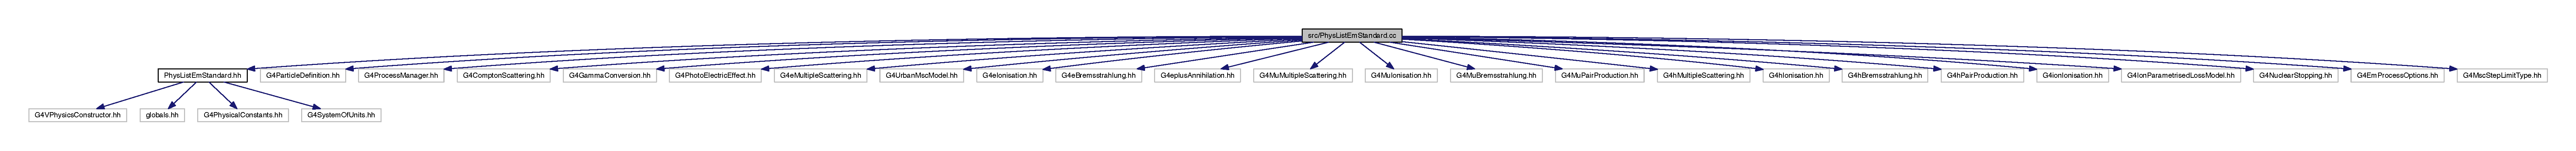
\includegraphics[width=350pt]{PhysListEmStandard_8cc__incl}
\end{center}
\end{figure}

\hypertarget{RunAction_8cc}{}\section{src/\+Run\+Action.cc File Reference}
\label{RunAction_8cc}\index{src/\+Run\+Action.\+cc@{src/\+Run\+Action.\+cc}}
{\ttfamily \#include \char`\"{}Run\+Action.\+hh\char`\"{}}\\*
{\ttfamily \#include \char`\"{}U\+M\+Event\+Action.\+hh\char`\"{}}\\*
{\ttfamily \#include \char`\"{}U\+M\+Root\+Saver.\+hh\char`\"{}}\\*
{\ttfamily \#include \char`\"{}G4\+Run.\+hh\char`\"{}}\\*
{\ttfamily \#include $<$sstream$>$}\\*
{\ttfamily \#include $<$iostream$>$}\\*
Include dependency graph for Run\+Action.\+cc\+:
\nopagebreak
\begin{figure}[H]
\begin{center}
\leavevmode
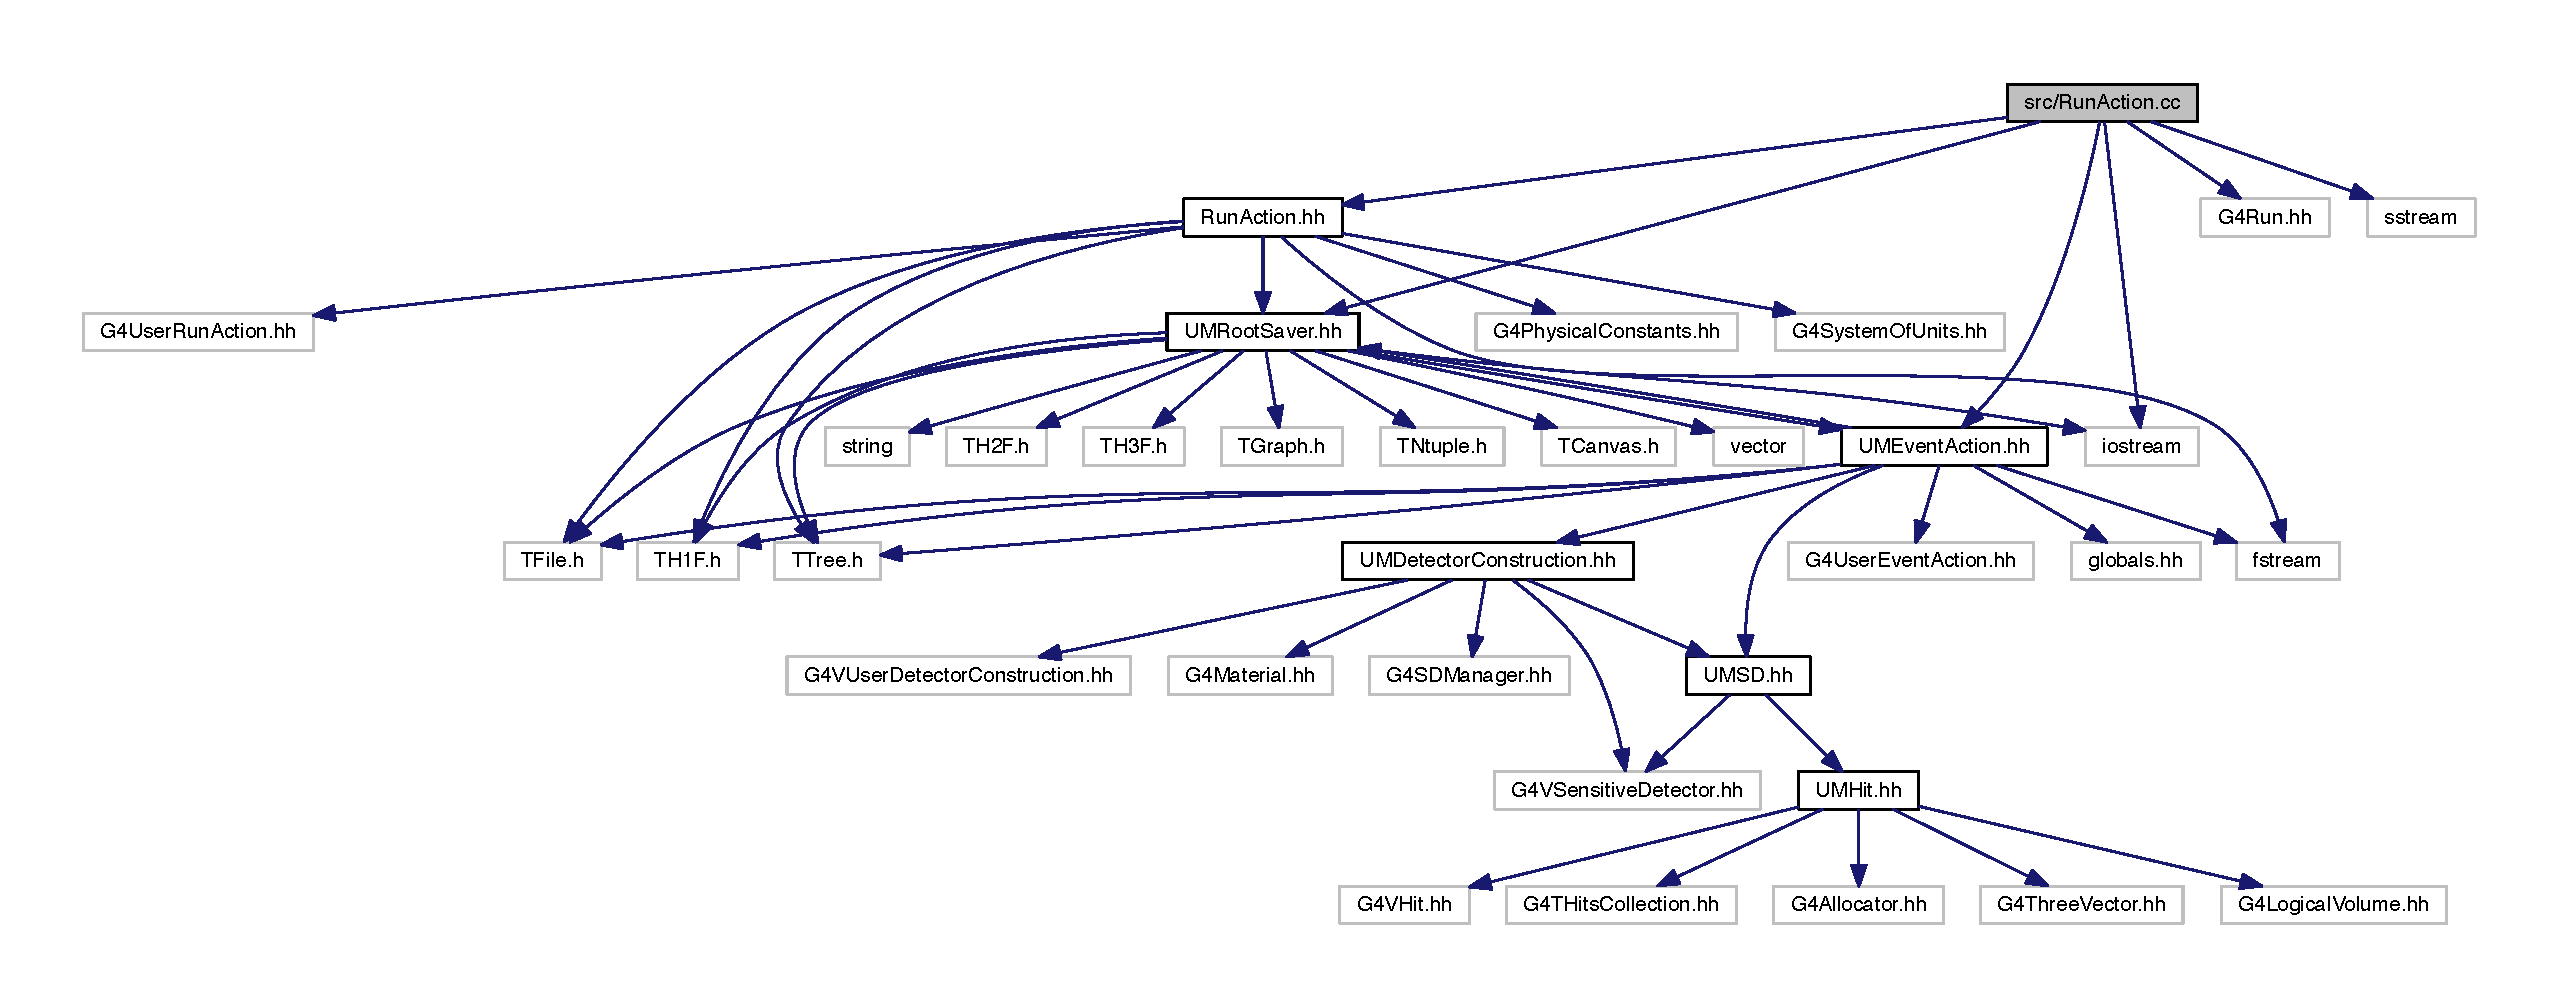
\includegraphics[width=350pt]{RunAction_8cc__incl}
\end{center}
\end{figure}

\hypertarget{UMConfig_8cc}{}\section{src/\+U\+M\+Config.cc File Reference}
\label{UMConfig_8cc}\index{src/\+U\+M\+Config.\+cc@{src/\+U\+M\+Config.\+cc}}
{\ttfamily \#include \char`\"{}U\+M\+Config.\+hh\char`\"{}}\\*
Include dependency graph for U\+M\+Config.\+cc\+:
\nopagebreak
\begin{figure}[H]
\begin{center}
\leavevmode
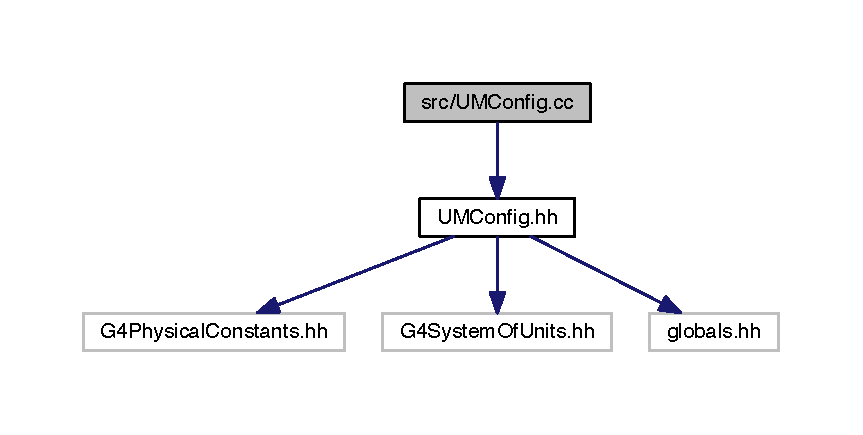
\includegraphics[width=350pt]{UMConfig_8cc__incl}
\end{center}
\end{figure}
\subsection*{Variables}
\begin{DoxyCompactItemize}
\item 
struct \hyperlink{structUMConfig}{U\+M\+Config} \hyperlink{UMConfig_8cc_ac76e235bdd1e4508d33696b9ae7bff7b}{config}
\end{DoxyCompactItemize}


\subsection{Variable Documentation}
\hypertarget{UMConfig_8cc_ac76e235bdd1e4508d33696b9ae7bff7b}{}\index{U\+M\+Config.\+cc@{U\+M\+Config.\+cc}!config@{config}}
\index{config@{config}!U\+M\+Config.\+cc@{U\+M\+Config.\+cc}}
\subsubsection[{config}]{\setlength{\rightskip}{0pt plus 5cm}struct {\bf U\+M\+Config} config}\label{UMConfig_8cc_ac76e235bdd1e4508d33696b9ae7bff7b}
Dummy source for \begin{DoxySeeAlso}{See also}
\hyperlink{structUMConfig}{U\+M\+Config}
\end{DoxySeeAlso}
\begin{DoxyAuthor}{Author}
Nikolaos Karastathis $<$ nkarast .at. cern .dot. ch $>$ 
\end{DoxyAuthor}
\begin{DoxyVersion}{Version}
v2.\+0 
\end{DoxyVersion}

\hypertarget{UMDetectorConstruction_8cc}{}\section{src/\+U\+M\+Detector\+Construction.cc File Reference}
\label{UMDetectorConstruction_8cc}\index{src/\+U\+M\+Detector\+Construction.\+cc@{src/\+U\+M\+Detector\+Construction.\+cc}}
{\ttfamily \#include \char`\"{}U\+M\+Detector\+Construction.\+hh\char`\"{}}\\*
{\ttfamily \#include \char`\"{}G4\+Box.\+hh\char`\"{}}\\*
{\ttfamily \#include \char`\"{}G4\+Tubs.\+hh\char`\"{}}\\*
{\ttfamily \#include \char`\"{}G4\+Logical\+Volume.\+hh\char`\"{}}\\*
{\ttfamily \#include \char`\"{}G4\+V\+Physical\+Volume.\+hh\char`\"{}}\\*
{\ttfamily \#include \char`\"{}G4\+P\+V\+Placement.\+hh\char`\"{}}\\*
{\ttfamily \#include \char`\"{}G4\+P\+V\+Replica.\+hh\char`\"{}}\\*
{\ttfamily \#include \char`\"{}globals.\+hh\char`\"{}}\\*
{\ttfamily \#include \char`\"{}G4\+Three\+Vector.\+hh\char`\"{}}\\*
{\ttfamily \#include \char`\"{}G4\+Material.\+hh\char`\"{}}\\*
{\ttfamily \#include \char`\"{}G4\+V\+Solid.\+hh\char`\"{}}\\*
{\ttfamily \#include \char`\"{}G4\+Extruded\+Solid.\+hh\char`\"{}}\\*
{\ttfamily \#include \char`\"{}G4\+Subtraction\+Solid.\+hh\char`\"{}}\\*
{\ttfamily \#include \char`\"{}G4\+Nist\+Manager.\+hh\char`\"{}}\\*
{\ttfamily \#include \char`\"{}G4\+Vis\+Attributes.\+hh\char`\"{}}\\*
{\ttfamily \#include \char`\"{}G4\+Colour.\+hh\char`\"{}}\\*
{\ttfamily \#include \char`\"{}G4ios.\+hh\char`\"{}}\\*
{\ttfamily \#include \char`\"{}G4\+S\+D\+Manager.\+hh\char`\"{}}\\*
{\ttfamily \#include \char`\"{}G4\+V\+Sensitive\+Detector.\+hh\char`\"{}}\\*
{\ttfamily \#include \char`\"{}U\+M\+S\+D.\+hh\char`\"{}}\\*
{\ttfamily \#include \char`\"{}G4\+Physical\+Constants.\+hh\char`\"{}}\\*
{\ttfamily \#include \char`\"{}G4\+System\+Of\+Units.\+hh\char`\"{}}\\*
{\ttfamily \#include \char`\"{}G4\+P\+V\+Parameterised.\+hh\char`\"{}}\\*
{\ttfamily \#include \char`\"{}U\+M\+Config.\+hh\char`\"{}}\\*
Include dependency graph for U\+M\+Detector\+Construction.\+cc\+:
\nopagebreak
\begin{figure}[H]
\begin{center}
\leavevmode
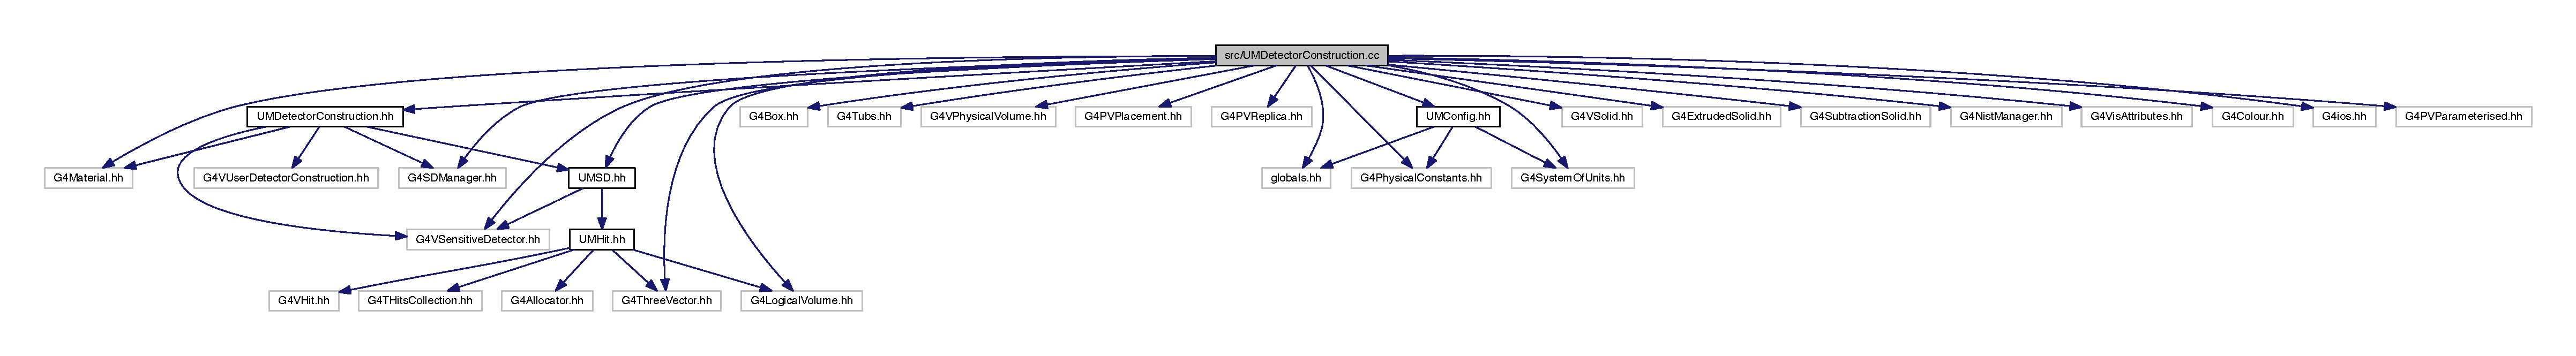
\includegraphics[width=350pt]{UMDetectorConstruction_8cc__incl}
\end{center}
\end{figure}

\hypertarget{UMEventAction_8cc}{}\section{src/\+U\+M\+Event\+Action.cc File Reference}
\label{UMEventAction_8cc}\index{src/\+U\+M\+Event\+Action.\+cc@{src/\+U\+M\+Event\+Action.\+cc}}
{\ttfamily \#include \char`\"{}U\+M\+Event\+Action.\+hh\char`\"{}}\\*
{\ttfamily \#include \char`\"{}U\+M\+Root\+Saver.\+hh\char`\"{}}\\*
{\ttfamily \#include \char`\"{}U\+M\+Hit.\+hh\char`\"{}}\\*
{\ttfamily \#include \char`\"{}U\+M\+S\+D.\+hh\char`\"{}}\\*
{\ttfamily \#include \char`\"{}G4\+Event.\+hh\char`\"{}}\\*
{\ttfamily \#include \char`\"{}G4\+Event\+Manager.\+hh\char`\"{}}\\*
{\ttfamily \#include \char`\"{}G4\+H\+Cof\+This\+Event.\+hh\char`\"{}}\\*
{\ttfamily \#include \char`\"{}G4\+V\+Hits\+Collection.\+hh\char`\"{}}\\*
{\ttfamily \#include \char`\"{}G4\+S\+D\+Manager.\+hh\char`\"{}}\\*
{\ttfamily \#include \char`\"{}G4\+Units\+Table.\+hh\char`\"{}}\\*
{\ttfamily \#include \char`\"{}globals.\+hh\char`\"{}}\\*
{\ttfamily \#include \char`\"{}G4\+Physical\+Constants.\+hh\char`\"{}}\\*
{\ttfamily \#include \char`\"{}G4\+System\+Of\+Units.\+hh\char`\"{}}\\*
{\ttfamily \#include \char`\"{}G4ios.\+hh\char`\"{}}\\*
{\ttfamily \#include \char`\"{}U\+M\+Config.\+hh\char`\"{}}\\*
{\ttfamily \#include $<$fstream$>$}\\*
{\ttfamily \#include $<$iostream$>$}\\*
{\ttfamily \#include \char`\"{}T\+R\+O\+O\+T.\+h\char`\"{}}\\*
{\ttfamily \#include \char`\"{}T\+File.\+h\char`\"{}}\\*
{\ttfamily \#include \char`\"{}T\+Tree.\+h\char`\"{}}\\*
Include dependency graph for U\+M\+Event\+Action.\+cc\+:
\nopagebreak
\begin{figure}[H]
\begin{center}
\leavevmode
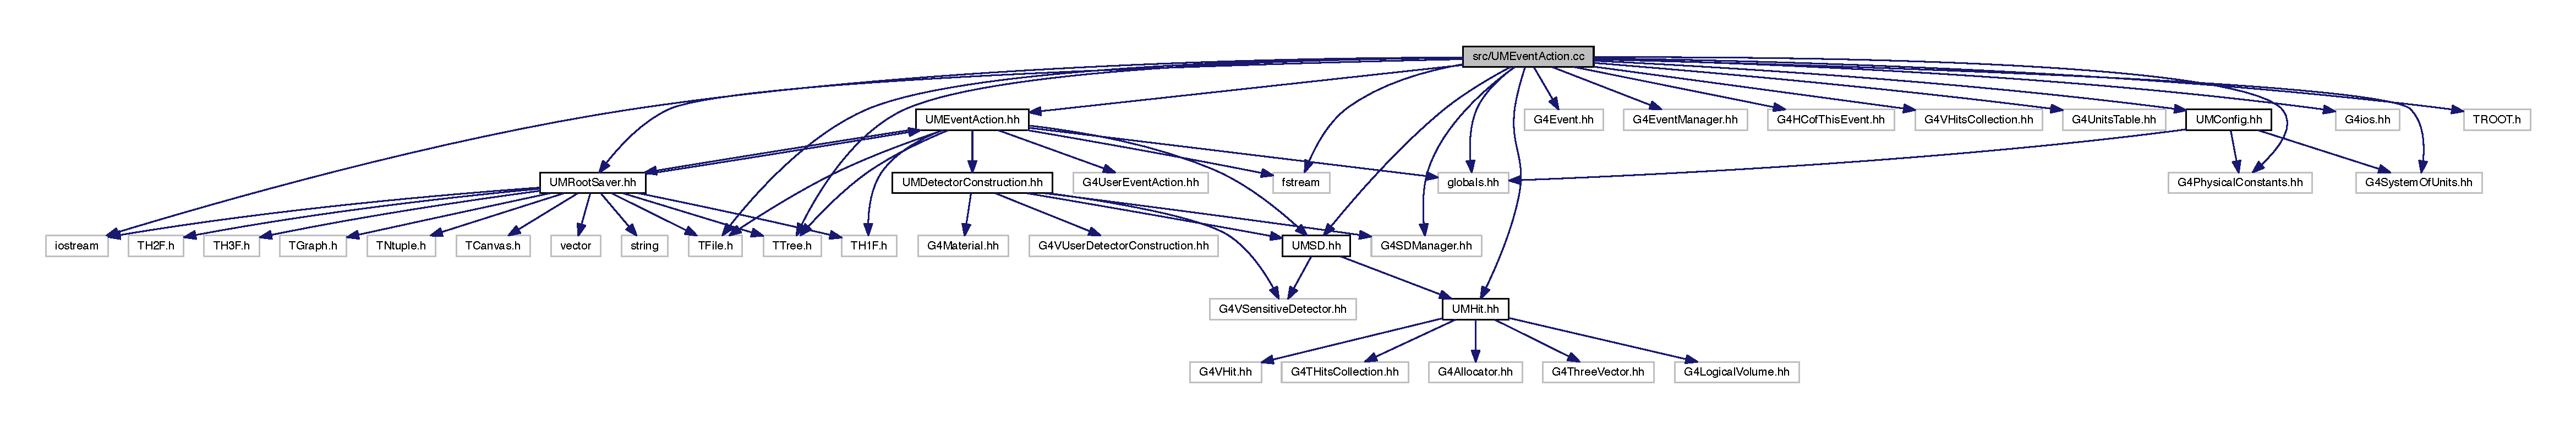
\includegraphics[width=350pt]{UMEventAction_8cc__incl}
\end{center}
\end{figure}

\hypertarget{UMHit_8cc}{}\section{src/\+U\+M\+Hit.cc File Reference}
\label{UMHit_8cc}\index{src/\+U\+M\+Hit.\+cc@{src/\+U\+M\+Hit.\+cc}}
{\ttfamily \#include \char`\"{}U\+M\+Hit.\+hh\char`\"{}}\\*
{\ttfamily \#include \char`\"{}U\+M\+S\+D.\+hh\char`\"{}}\\*
{\ttfamily \#include \char`\"{}G4ios.\+hh\char`\"{}}\\*
{\ttfamily \#include \char`\"{}globals.\+hh\char`\"{}}\\*
{\ttfamily \#include \char`\"{}G4\+Physical\+Constants.\+hh\char`\"{}}\\*
{\ttfamily \#include \char`\"{}G4\+System\+Of\+Units.\+hh\char`\"{}}\\*
{\ttfamily \#include \char`\"{}G4\+V\+Vis\+Manager.\+hh\char`\"{}}\\*
{\ttfamily \#include \char`\"{}G4\+Circle.\+hh\char`\"{}}\\*
{\ttfamily \#include \char`\"{}G4\+Colour.\+hh\char`\"{}}\\*
{\ttfamily \#include \char`\"{}G4\+Units\+Table.\+hh\char`\"{}}\\*
{\ttfamily \#include \char`\"{}G4\+Vis\+Attributes.\+hh\char`\"{}}\\*
{\ttfamily \#include $<$iostream$>$}\\*
{\ttfamily \#include $<$fstream$>$}\\*
Include dependency graph for U\+M\+Hit.\+cc\+:
\nopagebreak
\begin{figure}[H]
\begin{center}
\leavevmode
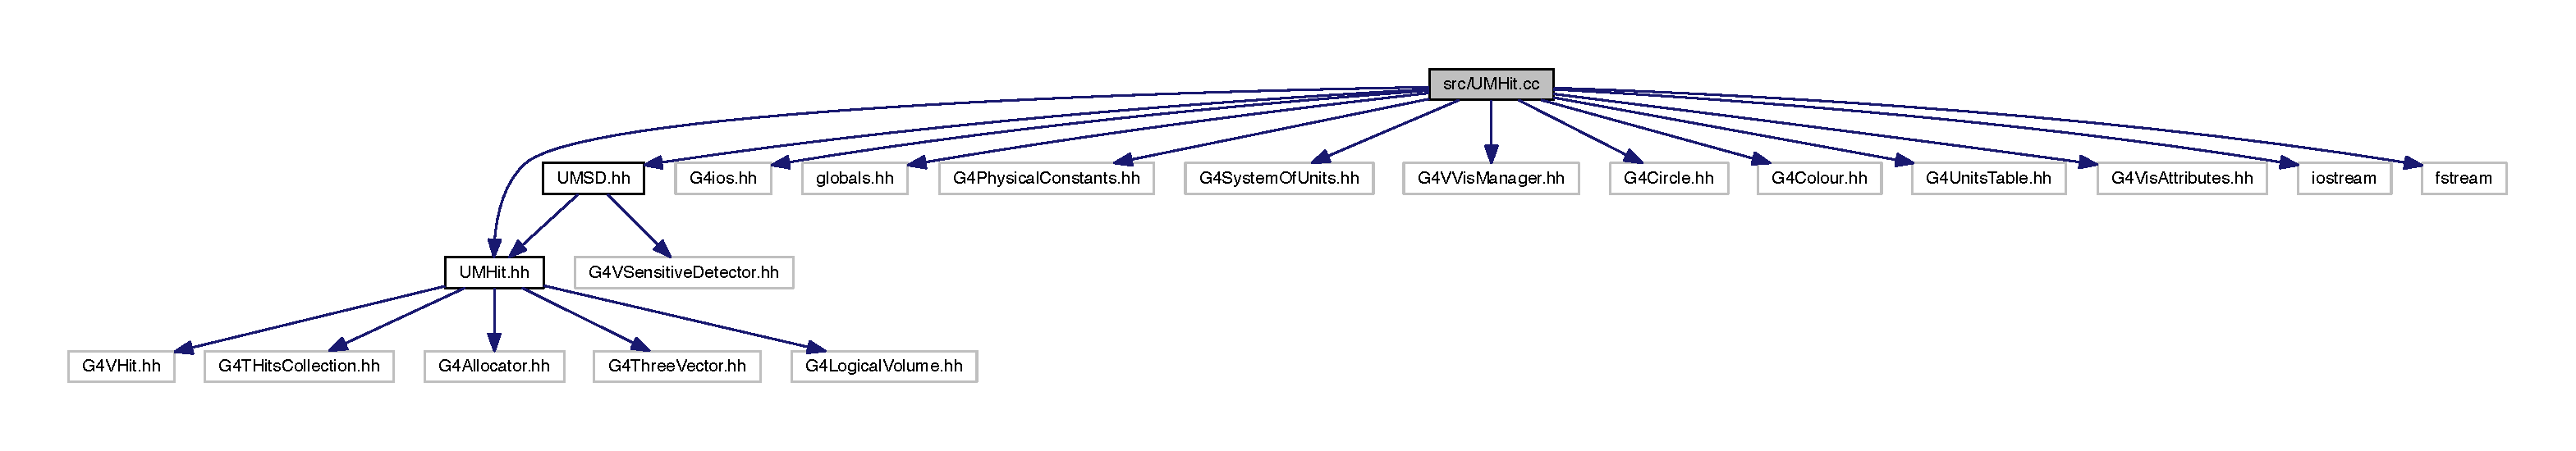
\includegraphics[width=350pt]{UMHit_8cc__incl}
\end{center}
\end{figure}
\subsection*{Variables}
\begin{DoxyCompactItemize}
\item 
G4\+Allocator$<$ \hyperlink{classUMHit}{U\+M\+Hit} $>$ \hyperlink{UMHit_8cc_a9d8361bd2d8e805dd16550d0d0808c57}{U\+M\+Hit\+Allocator}
\begin{DoxyCompactList}\small\item\em new and delete overloaded operators\+: \end{DoxyCompactList}\end{DoxyCompactItemize}


\subsection{Variable Documentation}
\hypertarget{UMHit_8cc_a9d8361bd2d8e805dd16550d0d0808c57}{}\index{U\+M\+Hit.\+cc@{U\+M\+Hit.\+cc}!U\+M\+Hit\+Allocator@{U\+M\+Hit\+Allocator}}
\index{U\+M\+Hit\+Allocator@{U\+M\+Hit\+Allocator}!U\+M\+Hit.\+cc@{U\+M\+Hit.\+cc}}
\subsubsection[{U\+M\+Hit\+Allocator}]{\setlength{\rightskip}{0pt plus 5cm}G4\+Allocator$<${\bf U\+M\+Hit}$>$ U\+M\+Hit\+Allocator}\label{UMHit_8cc_a9d8361bd2d8e805dd16550d0d0808c57}


new and delete overloaded operators\+: 


\hypertarget{UMPhysicsList_8cc}{}\section{src/\+U\+M\+Physics\+List.cc File Reference}
\label{UMPhysicsList_8cc}\index{src/\+U\+M\+Physics\+List.\+cc@{src/\+U\+M\+Physics\+List.\+cc}}
{\ttfamily \#include \char`\"{}U\+M\+Physics\+List.\+hh\char`\"{}}\\*
{\ttfamily \#include \char`\"{}globals.\+hh\char`\"{}}\\*
{\ttfamily \#include \char`\"{}G4\+Physical\+Constants.\+hh\char`\"{}}\\*
{\ttfamily \#include \char`\"{}G4\+System\+Of\+Units.\+hh\char`\"{}}\\*
{\ttfamily \#include \char`\"{}G4\+Em\+Penelope\+Physics.\+hh\char`\"{}}\\*
{\ttfamily \#include \char`\"{}G4\+Decay\+Physics.\+hh\char`\"{}}\\*
{\ttfamily \#include \char`\"{}G4\+Loss\+Table\+Manager.\+hh\char`\"{}}\\*
{\ttfamily \#include \char`\"{}G4\+Process\+Manager.\+hh\char`\"{}}\\*
{\ttfamily \#include \char`\"{}G4\+Particle\+Types.\+hh\char`\"{}}\\*
{\ttfamily \#include \char`\"{}G4\+Charged\+Geantino.\+hh\char`\"{}}\\*
{\ttfamily \#include \char`\"{}G4\+Geantino.\+hh\char`\"{}}\\*
{\ttfamily \#include \char`\"{}G4\+Gamma.\+hh\char`\"{}}\\*
{\ttfamily \#include \char`\"{}G4\+Optical\+Photon.\+hh\char`\"{}}\\*
{\ttfamily \#include \char`\"{}G4\+Muon\+Plus.\+hh\char`\"{}}\\*
{\ttfamily \#include \char`\"{}G4\+Muon\+Minus.\+hh\char`\"{}}\\*
{\ttfamily \#include \char`\"{}G4\+Neutrino\+Mu.\+hh\char`\"{}}\\*
{\ttfamily \#include \char`\"{}G4\+Anti\+Neutrino\+Mu.\+hh\char`\"{}}\\*
{\ttfamily \#include \char`\"{}G4\+Electron.\+hh\char`\"{}}\\*
{\ttfamily \#include \char`\"{}G4\+Positron.\+hh\char`\"{}}\\*
{\ttfamily \#include \char`\"{}G4\+Neutrino\+E.\+hh\char`\"{}}\\*
{\ttfamily \#include \char`\"{}G4\+Anti\+Neutrino\+E.\+hh\char`\"{}}\\*
{\ttfamily \#include \char`\"{}G4\+Pion\+Plus.\+hh\char`\"{}}\\*
{\ttfamily \#include \char`\"{}G4\+Pion\+Minus.\+hh\char`\"{}}\\*
{\ttfamily \#include \char`\"{}G4\+Pion\+Zero.\+hh\char`\"{}}\\*
{\ttfamily \#include \char`\"{}G4\+Eta.\+hh\char`\"{}}\\*
{\ttfamily \#include \char`\"{}G4\+Eta\+Prime.\+hh\char`\"{}}\\*
{\ttfamily \#include \char`\"{}G4\+Kaon\+Plus.\+hh\char`\"{}}\\*
{\ttfamily \#include \char`\"{}G4\+Kaon\+Minus.\+hh\char`\"{}}\\*
{\ttfamily \#include \char`\"{}G4\+Kaon\+Zero.\+hh\char`\"{}}\\*
{\ttfamily \#include \char`\"{}G4\+Anti\+Kaon\+Zero.\+hh\char`\"{}}\\*
{\ttfamily \#include \char`\"{}G4\+Kaon\+Zero\+Long.\+hh\char`\"{}}\\*
{\ttfamily \#include \char`\"{}G4\+Kaon\+Zero\+Short.\+hh\char`\"{}}\\*
{\ttfamily \#include \char`\"{}G4\+Proton.\+hh\char`\"{}}\\*
{\ttfamily \#include \char`\"{}G4\+Anti\+Proton.\+hh\char`\"{}}\\*
{\ttfamily \#include \char`\"{}G4\+Neutron.\+hh\char`\"{}}\\*
{\ttfamily \#include \char`\"{}G4\+Anti\+Neutron.\+hh\char`\"{}}\\*
{\ttfamily \#include \char`\"{}G4\+Alpha.\+hh\char`\"{}}\\*
{\ttfamily \#include \char`\"{}G4\+Deuteron.\+hh\char`\"{}}\\*
{\ttfamily \#include \char`\"{}G4\+Triton.\+hh\char`\"{}}\\*
{\ttfamily \#include \char`\"{}G4\+He3.\+hh\char`\"{}}\\*
{\ttfamily \#include \char`\"{}G4\+Generic\+Ion.\+hh\char`\"{}}\\*
{\ttfamily \#include \char`\"{}G4\+Decay.\+hh\char`\"{}}\\*
Include dependency graph for U\+M\+Physics\+List.\+cc\+:
\nopagebreak
\begin{figure}[H]
\begin{center}
\leavevmode

\includegraphics[width=350pt]{UMPhysicsList_8cc__incl}
\end{center}
\end{figure}

\hypertarget{UMPrimaryGeneratorAction_8cc}{}\section{src/\+U\+M\+Primary\+Generator\+Action.cc File Reference}
\label{UMPrimaryGeneratorAction_8cc}\index{src/\+U\+M\+Primary\+Generator\+Action.\+cc@{src/\+U\+M\+Primary\+Generator\+Action.\+cc}}
{\ttfamily \#include \char`\"{}U\+M\+Primary\+Generator\+Action.\+hh\char`\"{}}\\*
{\ttfamily \#include \char`\"{}U\+M\+Detector\+Construction.\+hh\char`\"{}}\\*
{\ttfamily \#include \char`\"{}Randomize.\+hh\char`\"{}}\\*
{\ttfamily \#include \char`\"{}globals.\+hh\char`\"{}}\\*
{\ttfamily \#include \char`\"{}G4\+Physical\+Constants.\+hh\char`\"{}}\\*
{\ttfamily \#include \char`\"{}G4\+System\+Of\+Units.\+hh\char`\"{}}\\*
{\ttfamily \#include \char`\"{}G4\+Particle\+Definition.\+hh\char`\"{}}\\*
{\ttfamily \#include \char`\"{}G4\+Particle\+Table.\+hh\char`\"{}}\\*
{\ttfamily \#include \char`\"{}G4\+Event.\+hh\char`\"{}}\\*
{\ttfamily \#include \char`\"{}G4\+Particle\+Gun.\+hh\char`\"{}}\\*
{\ttfamily \#include \char`\"{}U\+M\+Config.\+hh\char`\"{}}\\*
{\ttfamily \#include $<$fstream$>$}\\*
{\ttfamily \#include $<$iostream$>$}\\*
Include dependency graph for U\+M\+Primary\+Generator\+Action.\+cc\+:
\nopagebreak
\begin{figure}[H]
\begin{center}
\leavevmode
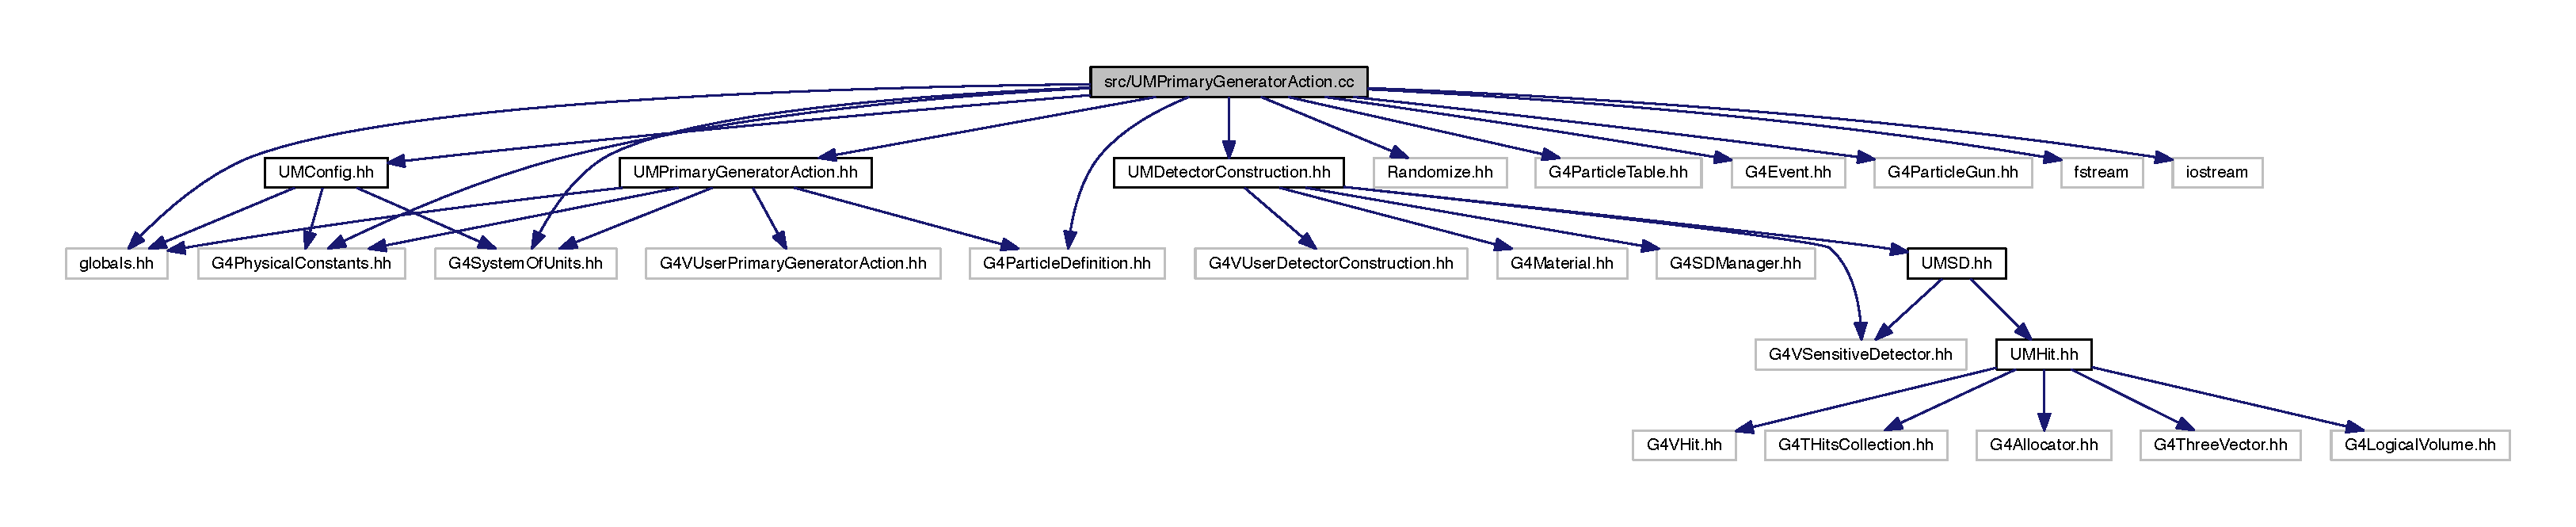
\includegraphics[width=350pt]{UMPrimaryGeneratorAction_8cc__incl}
\end{center}
\end{figure}

\hypertarget{UMRootSaver_8cc}{}\section{src/\+U\+M\+Root\+Saver.cc File Reference}
\label{UMRootSaver_8cc}\index{src/\+U\+M\+Root\+Saver.\+cc@{src/\+U\+M\+Root\+Saver.\+cc}}
{\ttfamily \#include \char`\"{}U\+M\+Root\+Saver.\+hh\char`\"{}}\\*
{\ttfamily \#include \char`\"{}U\+M\+Event\+Action.\+hh\char`\"{}}\\*
{\ttfamily \#include \char`\"{}G4\+Physical\+Constants.\+hh\char`\"{}}\\*
{\ttfamily \#include \char`\"{}G4\+System\+Of\+Units.\+hh\char`\"{}}\\*
{\ttfamily \#include \char`\"{}T\+Ntuple.\+h\char`\"{}}\\*
{\ttfamily \#include \char`\"{}T\+File.\+h\char`\"{}}\\*
{\ttfamily \#include \char`\"{}T\+Tree.\+h\char`\"{}}\\*
{\ttfamily \#include \char`\"{}T\+Graph.\+h\char`\"{}}\\*
{\ttfamily \#include \char`\"{}T\+Canvas.\+h\char`\"{}}\\*
{\ttfamily \#include \char`\"{}T\+H1\+F.\+h\char`\"{}}\\*
{\ttfamily \#include $<$T\+H2\+F.\+h$>$}\\*
{\ttfamily \#include \char`\"{}T\+Math.\+h\char`\"{}}\\*
{\ttfamily \#include $<$sstream$>$}\\*
{\ttfamily \#include $<$cassert$>$}\\*
{\ttfamily \#include $<$string$>$}\\*
{\ttfamily \#include \char`\"{}U\+M\+Config.\+hh\char`\"{}}\\*
Include dependency graph for U\+M\+Root\+Saver.\+cc\+:
\nopagebreak
\begin{figure}[H]
\begin{center}
\leavevmode
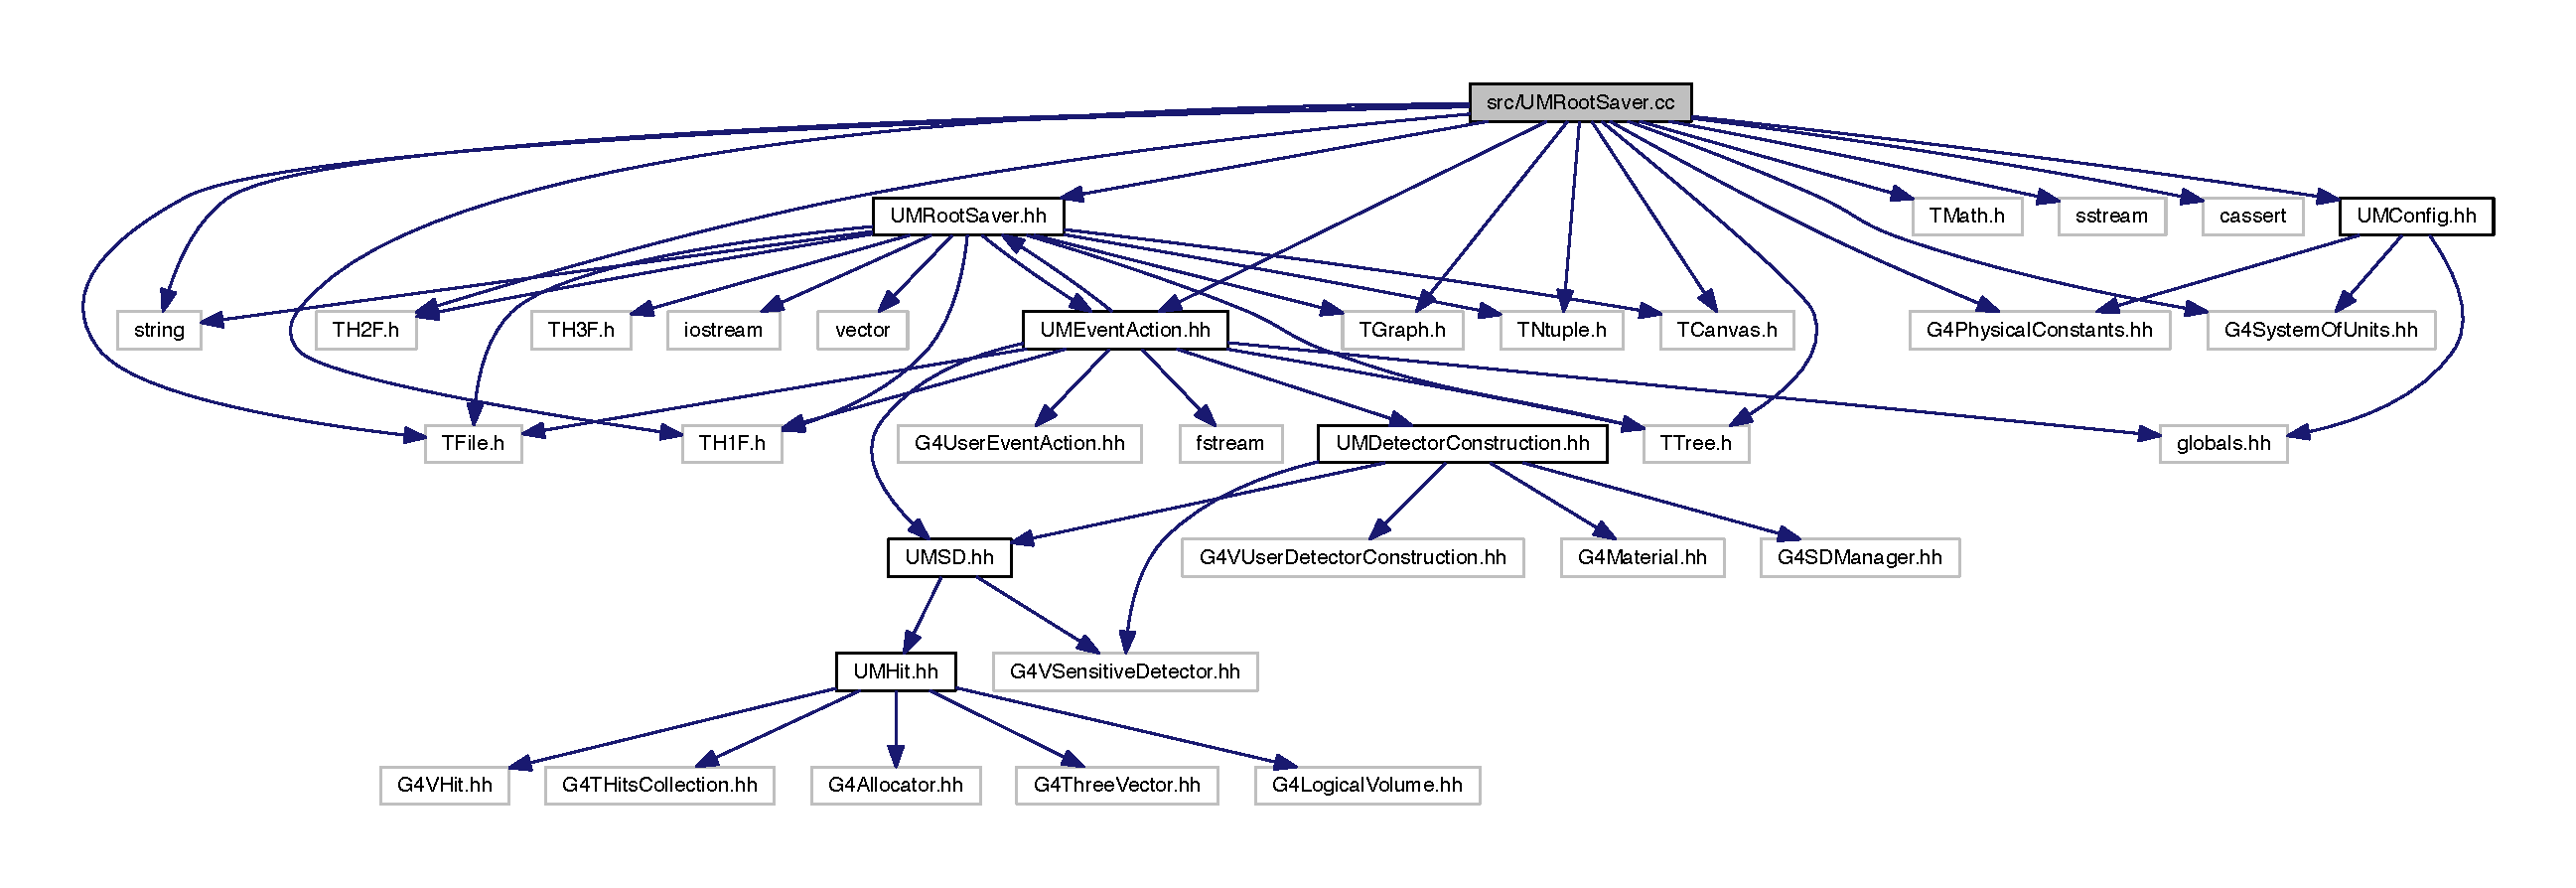
\includegraphics[width=350pt]{UMRootSaver_8cc__incl}
\end{center}
\end{figure}

\hypertarget{UMSD_8cc}{}\section{src/\+U\+M\+S\+D.cc File Reference}
\label{UMSD_8cc}\index{src/\+U\+M\+S\+D.\+cc@{src/\+U\+M\+S\+D.\+cc}}
{\ttfamily \#include \char`\"{}U\+M\+S\+D.\+hh\char`\"{}}\\*
{\ttfamily \#include \char`\"{}U\+M\+Hit.\+hh\char`\"{}}\\*
{\ttfamily \#include \char`\"{}G4\+H\+Cof\+This\+Event.\+hh\char`\"{}}\\*
{\ttfamily \#include \char`\"{}G4\+Touchable\+History.\+hh\char`\"{}}\\*
{\ttfamily \#include \char`\"{}G4\+Step.\+hh\char`\"{}}\\*
{\ttfamily \#include \char`\"{}G4\+S\+D\+Manager.\+hh\char`\"{}}\\*
{\ttfamily \#include $<$fstream$>$}\\*
{\ttfamily \#include $<$iostream$>$}\\*
{\ttfamily \#include \char`\"{}G4\+Track.\+hh\char`\"{}}\\*
{\ttfamily \#include \char`\"{}G4\+V\+Process.\+hh\char`\"{}}\\*
Include dependency graph for U\+M\+S\+D.\+cc\+:
\nopagebreak
\begin{figure}[H]
\begin{center}
\leavevmode
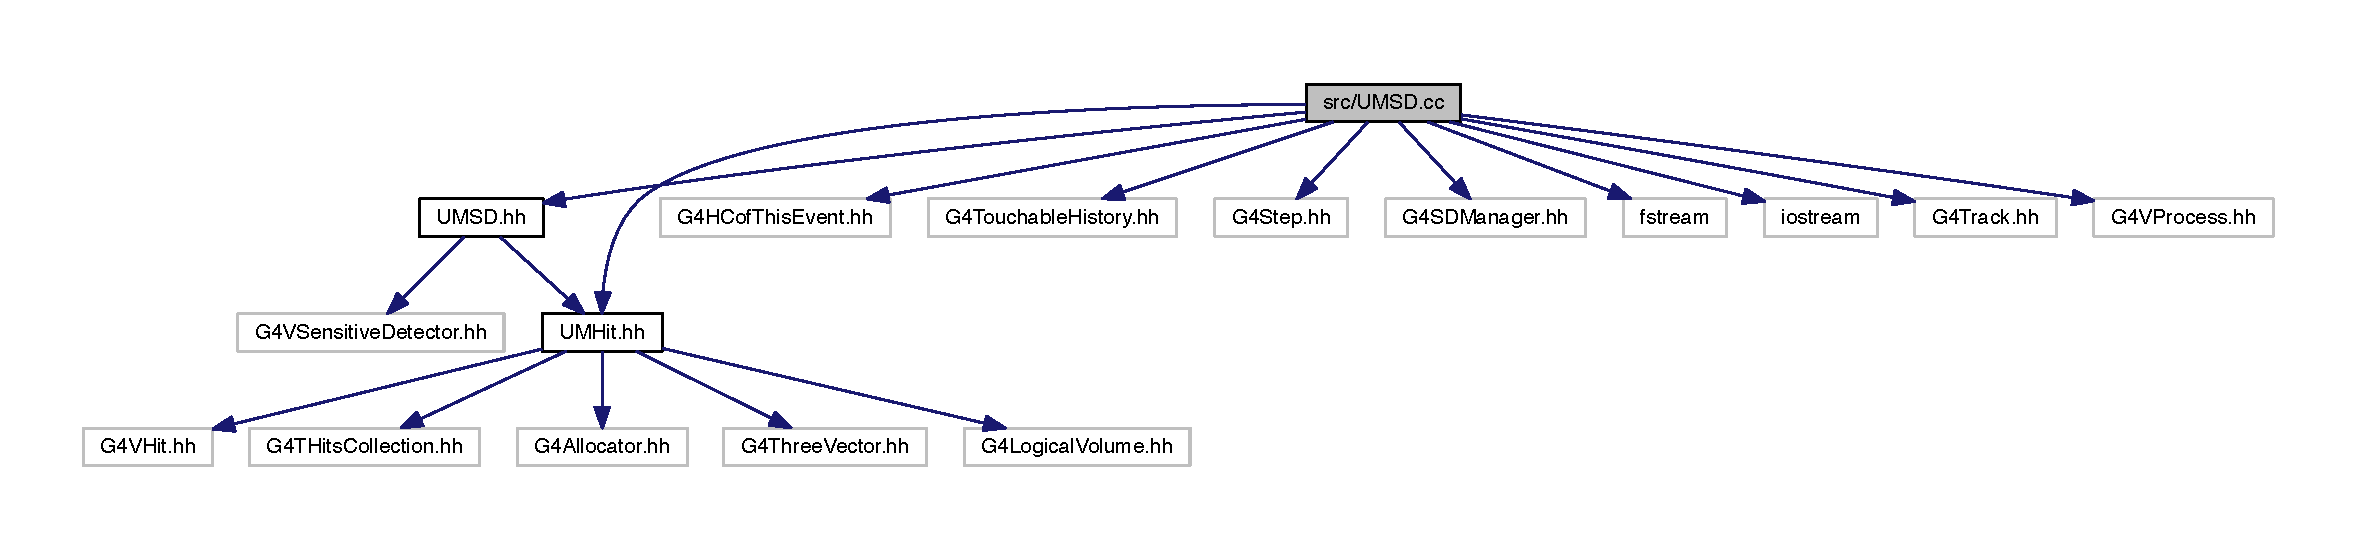
\includegraphics[width=350pt]{UMSD_8cc__incl}
\end{center}
\end{figure}

\hypertarget{UMVisManager_8cc}{}\section{src/\+U\+M\+Vis\+Manager.cc File Reference}
\label{UMVisManager_8cc}\index{src/\+U\+M\+Vis\+Manager.\+cc@{src/\+U\+M\+Vis\+Manager.\+cc}}

%--- End generated contents ---

% Index
\backmatter
\newpage
\phantomsection
\clearemptydoublepage
\addcontentsline{toc}{chapter}{Index}
\printindex

\end{document}
